\clearpage
\bookpart{概率分布的优化与逼近}{Optimization and Approximation of Distributions}
\label{part:distribution-optimization}

\BookPartGuide{%
有时概率分布本身就是要求的未知量：在给定均值的条件下选一个最“平”的分布，用简单的分布近似一个难以计算的分布，或者以最低的成本把一堆质量搬成另一种形状。

第~\ref{chap:distribution-selection}章把分布作为优化变量，研究带 KL 代价的成本最小化、矩约束下的最小 KL 与最大熵。第~\ref{chap:distribution-approximation}章在给定目标分布后限制候选集合，研究逼近的目标、求解方法与误差。第~\ref{chap:information-geometry}章研究参数变化引起的分布变化，用 Fisher 信息给出局部尺度，再把分布变化的限制转成参数的更新方向。第~\ref{chap:optimal-transport}章固定两个边缘分布，在所有耦合中寻找成本最低的运输方案，并研究由此得到的分布距离、插值与重心。}

\chapter{概率分布的选择}
\label{chap:distribution-selection}

一个随机结果只取$0,1,2$三个值，原来的规律是三者等可能。现在希望改动这张概率表。若只想让结果的平均值尽量小，把全部概率放到$0$上就够了，可这样一来原来可能出现的$1$和$2$再也不会出现。若要求平均值恰好是$10/7$，满足要求的概率表有无穷多张。若只要求离原表近，那么不改最好。三种愿望各自给出的答案要么太极端，要么不唯一，要么什么也没做。

前几章研究的是给定的分布：怎样描述它、怎样比较两个分布、怎样度量它的不确定性。本章反过来，把概率分布本身当作未知量，在允许的分布中按某个目标选出一个。待求的不再是几个参数，而是一整张概率表，甚至是一个一般的概率测度；目标是概率表的函数，约束是概率表必须满足的等式。

本章的路线如下。第一节先说清楚“允许哪些分布”和“目标是什么”，并检查目标是否有定义。第二节在成本与“偏离参考分布的代价”之间权衡，得到按成本指数加权的Gibbs分布。第三节不要成本，而要求选出的分布满足给定的平均量，在其中找离参考分布最近的一个；解是参考分布的指数倾斜，求它归结为一个矩匹配方程。第四节以熵为目标，在有限状态上它与第三节只差一个常数，在连续情形则必须先固定计算密度所用的参考测度。

三类问题的解都长成“参考分布乘以指数权重再归一化”的样子，这一形式是由最优性推出来的，不是事先假定的。公式给出的只是候选，第五节回到原问题，检查候选是否是合法的分布、是否满足约束、最小值是否存在以及是否被候选达到。本章使用第~\ref{chap:distribution-families}章的指数族与对数配分函数，第~\ref{chap:distribution-comparison}章的KL散度和第~\ref{chap:information-measures}章的熵。

\section{分布优化问题}
\label{sec:dsel-problems}

章首的三种愿望听起来都合理，可它们在数学上扮演的角色不同：有的是要尽量减小的量，有的是必须满足的等式，有的是不愿付出的代价。在写任何公式之前，先把它们在同一个小例子里分别算清楚，再规定一个分布优化问题由哪些部分组成。

\paragraph{三种不同的要求}
取$\mathcal{X}=\{0,1,2\}$，参考分布$P$是均匀分布，三个概率都是$1/3$。待选的分布$Q$由三个数$q(0),q(1),q(2)$给出，它们非负且和为$1$，全体这样的$Q$构成第~\ref{chap:distribution-families}章的概率三角形，三个顶点是单点分布$\delta_0,\delta_1,\delta_2$。设每个状态有一个成本$V(x)=x$。

第一种要求是降低期望成本。期望成本
\[
 \mathbb{E}_{Q}[V]=q(1)+2q(2)
\]
是$Q$的线性函数，它在三角形上的等值线是一族平行线。线性函数在三角形上的最小值一定在某个顶点取到，这里是$\delta_0$，最小值为$0$。这个答案把原本可能的状态$1$和$2$全部删掉了。若两个状态的成本相同且都最小，例如$V(0)=V(1)=0$，那么整条边上的分布都同样好，答案也不唯一。

第二种要求是满足指定的平均量，例如$\mathbb{E}_{Q}[X]=10/7$。它和归一化一起是三个未知数的两个线性方程：
\[
 q(1)+2q(2)=\frac{10}{7},\qquad q(0)+q(1)+q(2)=1 .
\]
令$q(1)=0$，解得$q(2)=5/7$，$q(0)=2/7$；令$q(0)=0$，解得$q(2)=3/7$，$q(1)=4/7$。满足要求的分布是连接$(\tfrac27,0,\tfrac57)$与$(0,\tfrac47,\tfrac37)$的一条线段，有无穷多个。约束本身不能从中挑出一个。

第三种要求是接近参考分布。用第~\ref{chap:distribution-comparison}章的KL散度衡量偏离，$D_{\mathrm{KL}}(Q\Vert P)\geq0$，且等号当且仅当$Q=P$。只最小化它，得到的就是$P$本身，什么也没有改变。

图~\ref{fig:dsel-three-requirements}把三种要求画在同一个三角形里。成本的等值线与平均量的约束线方向相同，因为这里成本和约束用的是同一个函数$x$，红色线段也就是期望成本等于$10/7$的那条等值线。只有把它们组合起来，例如“在红线上找离$P$最近的点”，问题才既不平凡又有确定的答案。

\begin{BookInlineFigure}
 \centering
 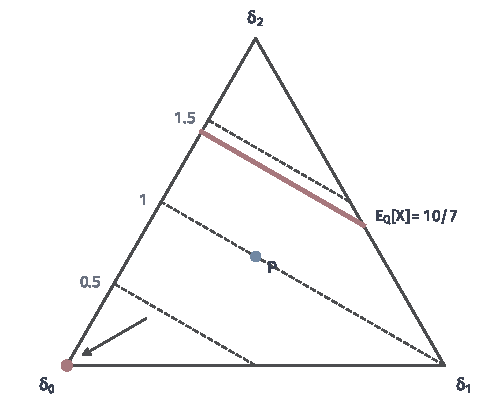
\includegraphics[width=84mm]{figures/07-probability/07-distribution-optimization/matplotlib/dsel-three-requirements/figure.pdf}
 \caption{$\{0,1,2\}$上的三种要求。三角形中每一点是一张概率表。深灰虚线是期望成本$\mathbb{E}_{Q}[V]=q(1)+2q(2)$的等值线，标注为取值，箭头指向成本最小的顶点$\delta_0$（红点）；红色线段是满足$\mathbb{E}_{Q}[X]=10/7$的全部分布；蓝点是参考分布$P$。}
 \label{fig:dsel-three-requirements}
\end{BookInlineFigure}

本章研究的三类问题正是这样的组合：
\begin{enumerate}
 \item 不加等式约束，最小化期望成本加上偏离参考分布的代价$\tau D_{\mathrm{KL}}(Q\Vert P)$，$\tau>0$调节两者的比重；
 \item 要求$\mathbb{E}_{Q}[\bm{T}]=\bm{m}$，在满足要求的分布中最小化$D_{\mathrm{KL}}(Q\Vert P)$；
 \item 要求$\mathbb{E}_{Q}[\bm{T}]=\bm{m}$，在满足要求的分布中最大化熵。
\end{enumerate}
其中$\bm{T}:\mathcal{X}\to\mathbb{R}^{k}$是若干个指定的统计量，$\bm{m}\in\mathbb{R}^{k}$是它们的指定平均值。

\paragraph{允许的分布}
一般情形下，$\mathcal{X}$是可测空间，记其上全体概率测度为$\mathcal{P}(\mathcal{X})$。待选对象是$\mathcal{P}(\mathcal{X})$中的元素，但并非每个元素都能参加比较。候选集合$\mathcal{Q}\subseteq\mathcal{P}(\mathcal{X})$是问题的一部分，要逐项写明。

非负性与归一化看起来理所当然，计算时却最容易丢掉。在上面的例子里，若只解那两个线性方程，以$q(1)=t$为参数，得到
\[
 q(2)=\frac57-\frac t2,\qquad q(0)=\frac27-\frac t2 .
\]
取$t=1$，得到$(-\tfrac{3}{14},1,\tfrac{3}{14})$。它和为$1$，平均值也是$10/7$，但$q(0)<0$，不是概率表。只有$0\leq t\leq4/7$才合法。凡是用方程、公式或数值迭代得出的“分布”，都要回头核对这两条。

其次是支持。若$Q$在$P$概率为零的地方放了质量，即$Q$不绝对连续于$P$，则$D_{\mathrm{KL}}(Q\Vert P)=+\infty$。所以只要目标里含有$D_{\mathrm{KL}}(Q\Vert P)$，有意义的候选都满足$Q\ll P$：选出的分布可以删去参考分布的状态，但不能添加新的状态。

最后是可积性。期望成本$\mathbb{E}_{Q}[V]$与约束中的$\mathbb{E}_{Q}[\bm{T}]$都要求相应函数在$Q$下可积，否则目标或约束不是一个确定的实数。有限状态上这一条自动成立，可数或连续状态上必须单独检查。

\begin{definition}[分布优化问题]
\label{def:dsel-problem}
设$\mathcal{Q}\subseteq\mathcal{P}(\mathcal{X})$是候选集合，$J:\mathcal{Q}\to(-\infty,+\infty]$。称
\begin{equation}
 J^{*}=\inf_{Q\in\mathcal{Q}}J(Q)
 \label{eq:dsel-problem}
\end{equation}
为\term{分布优化问题}（distribution optimization problem）的最优值。若$Q^{*}\in\mathcal{Q}$满足$J(Q^{*})=J^{*}$，称$Q^{*}$为\term{最优分布}（optimal distribution）。
\end{definition}

定义把三件事分开了。$\mathcal{Q}$非空且$J$在其上有定义，问题才成立；$J^{*}$可能是有限数，也可能是$-\infty$；即使$J^{*}$有限，也可能没有任何$Q$达到它。这三件事在第~\ref{sec:dsel-checks}节逐一检查，这里先看第一件事为什么不能省略。

\paragraph{无穷量不能相减}
目标$\mathbb{E}_{Q}[V]+\tau D_{\mathrm{KL}}(Q\Vert P)$由两项相加。第二项总在$[0,+\infty]$中；第一项若不加限制，可以是$-\infty$。下面的例子中两项分别是$-\infty$和$+\infty$。取$\mathcal{X}=\{1,2,\dots\}$，参考分布与成本为
\[
 P(k)=2^{-k},\qquad V(k)=-k ,
\]
候选分布取$Q(k)=\dfrac{6}{\pi^{2}k^{2}}$。

期望成本是调和级数乘以负数：
\[
 \mathbb{E}_{Q}[V]=-\frac{6}{\pi^{2}}\sum_{k\geq1}\frac1k=-\infty .
\]
再看对数比。对每个$k$，
\[
 \ln\frac{Q(k)}{P(k)}=\ln\frac{6}{\pi^{2}}-2\ln k+k\ln2 .
\]
按$Q$平均时，前两项给出收敛级数，因为$\sum_k(\ln k)/k^{2}<\infty$；第三项给出$\ln2\sum_kkQ(k)=+\infty$。所以$D_{\mathrm{KL}}(Q\Vert P)=+\infty$，目标成了“$-\infty+\infty$”。

把两个级数逐项配对，似乎能得到一个有限数。取$\tau=1/\ln2$，记前$N$项的部分和为
\[
 C_N=\sum_{k\leq N}Q(k)V(k),\qquad K_N=\tau\sum_{k\leq N}Q(k)\ln\frac{Q(k)}{P(k)} .
\]
这时$\tau k\ln2=k$，与$V(k)=-k$恰好抵消，$C_N+K_N$收敛到约$-2.363$。但若把$C_N$与$K_{2N}$配对，多出的部分是$\frac{6}{\pi^{2}}\sum_{N<k\leq2N}\frac1k$，它趋于$\frac{6}{\pi^{2}}\ln2\approx0.421$，极限变成约$-1.941$。图~\ref{fig:dsel-undefined-objective}画出了这几条部分和曲线。

\begin{BookInlineFigure}
 \centering
 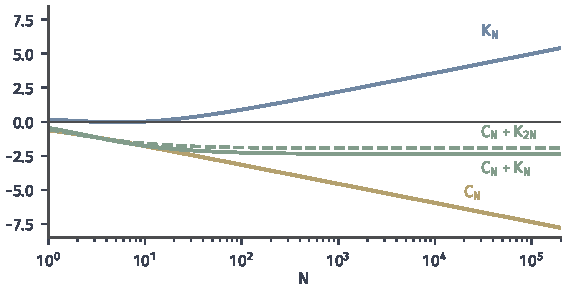
\includegraphics[width=96mm]{figures/07-probability/07-distribution-optimization/matplotlib/dsel-undefined-objective/figure.pdf}
 \caption{无定义的目标。$P(k)=2^{-k}$，$V(k)=-k$，$Q(k)=6/(\pi^{2}k^{2})$，$\tau=1/\ln2$，横轴为对数刻度。黄线是期望成本的部分和$C_N\to-\infty$，蓝线是KL项的部分和$K_N\to+\infty$；绿色实线$C_N+K_N$与绿色虚线$C_N+K_{2N}$各自收敛，极限相差$\frac{6}{\pi^{2}}\ln2\approx0.421$。}
 \label{fig:dsel-undefined-objective}
\end{BookInlineFigure}

一个数值若取决于怎样配对两条发散级数，它就不是目标函数的值。所以凡是目标含$\mathbb{E}_{Q}[V]+\tau D_{\mathrm{KL}}(Q\Vert P)$的问题，本章都把候选集合取为
\begin{equation}
 \mathcal{Q}_V=\Bigl\{Q\in\mathcal{P}(\mathcal{X}):\ D_{\mathrm{KL}}(Q\Vert P)<\infty,\ \mathbb{E}_{Q}\lvert V\rvert<\infty\Bigr\}.
 \label{eq:dsel-candidate-set}
\end{equation}
在$\mathcal{Q}_V$上两项都是有限实数，和有确定的值。有限状态且$P$处处为正时，$\mathcal{Q}_V$就是全部概率表。


\section{KL正则化的成本最小化}
\label{sec:dsel-kl-cost}

只降低期望成本，会把全部质量推到成本最低的状态上。若参考分布$P$代表原有的规律，我们愿意为降低成本而改动它，但改动本身也要付出代价。把这个代价记为$\tau D_{\mathrm{KL}}(Q\Vert P)$，$\tau>0$是一个换算系数：偏离参考分布一个nat，相当于多付$\tau$个单位的成本。

设$V:\mathcal{X}\to\mathbb{R}$可测，在每一点取有限值。在式~\eqref{eq:dsel-candidate-set}的候选集合上考虑
\begin{equation}
 \min_{Q\in\mathcal{Q}_V}\ J_\tau(Q),\qquad J_\tau(Q)=\mathbb{E}_{Q}[V]+\tau D_{\mathrm{KL}}(Q\Vert P).
 \label{eq:dsel-kl-cost-problem}
\end{equation}
在目标上加一个KL项以约束解不要离参考分布太远，这种做法称为\term{KL正则化}（KL regularization）。

\paragraph{有限状态上的权衡}
先在有限的$\mathcal{X}$上、$p(x)>0$处处成立时看目标的形状。这时
\[
 J_\tau(Q)=\sum_{x}q(x)V(x)+\tau\sum_{x}q(x)\ln\frac{q(x)}{p(x)} .
\]
第一项是线性的，它把质量拉向成本低的状态。第二项是凸的，而且函数$t\mapsto t\ln t$在$t\downarrow0$处的导数趋于$-\infty$：把某个状态的概率压到零，代价增长得极快。两者相抗，最优解应当留在三角形内部。

在内部，可以用归一化约束的Lagrange乘子$\nu$形式地求驻点。对$q(x)$求偏导并令其为零，得到
\[
 V(x)+\tau\Bigl(\ln\frac{q(x)}{p(x)}+1\Bigr)-\nu=0 .
\]
解出$q(x)$，
\[
 q(x)=p(x)\,\mathrm{e}^{-V(x)/\tau}\,\mathrm{e}^{\nu/\tau-1} .
\]
最后一个因子与$x$无关，由归一化确定。记$Z=\sum_xp(x)\mathrm{e}^{-V(x)/\tau}$，于是候选解是
\[
 q(x)=\frac{p(x)\,\mathrm{e}^{-V(x)/\tau}}{Z} .
\]
每个状态的参考概率乘上一个只由它自己的成本决定的权重$\mathrm{e}^{-V(x)/\tau}$，再整体归一。这一推导假设了解在内部且可微，只是猜测，下面将不借助导数直接验证它。

回到例子：$P$均匀，$V(x)=x$。取$\tau=1/\ln2$，权重就是$\mathrm{e}^{-V/\tau}=2^{-x}$，成本每多一个单位，权重减半。三个状态未归一的质量与归一化常数为
\[
 \frac13,\quad\frac16,\quad\frac1{12};\qquad Z=\frac13+\frac16+\frac1{12}=\frac7{12} .
\]
除以$Z$，得到
\[
 Q^{*}=\Bigl(\frac47,\ \frac27,\ \frac17\Bigr).
\]
图~\ref{fig:dsel-gibbs-bars}画出这一步：先乘权重，再归一化，质量从高成本状态挪向低成本状态，但没有任何状态被删去。

\begin{BookInlineFigure}
 \centering
 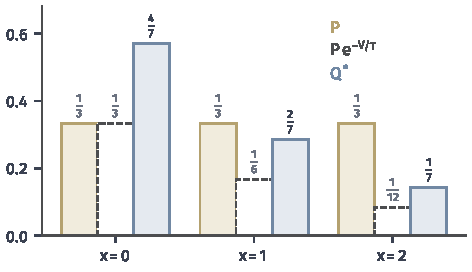
\includegraphics[width=80mm]{figures/07-probability/07-distribution-optimization/matplotlib/dsel-gibbs-bars/figure.pdf}
 \caption{按成本重新加权。$P$均匀（黄），$V(x)=x$，$\tau=1/\ln2$。白色虚线柱是未归一的$P\,\mathrm{e}^{-V/\tau}$，和为$Z=7/12$；蓝色柱是归一化后的$Q^{*}=(\frac47,\frac27,\frac17)$。}
 \label{fig:dsel-gibbs-bars}
\end{BookInlineFigure}

验证这个分布确实比别的好，先算它的目标值。期望成本是
\[
 \mathbb{E}_{Q^{*}}[V]=0\cdot\frac47+1\cdot\frac27+2\cdot\frac17=\frac47 .
\]
$P$的每个概率都是$1/3$，所以对数比是$\ln(3q^{*}(x))$，KL项为
\[
 D_{\mathrm{KL}}(Q^{*}\Vert P)=\frac47\ln\frac{12}7+\frac27\ln\frac67+\frac17\ln\frac37\approx0.3080-0.0440-0.1210=0.1429 .
\]
乘以$\tau=1/\ln2$后，KL项约为$0.2062$，相当于以比特计的偏离量。两项相加，
\[
 J_\tau(Q^{*})\approx0.5714+0.2062=0.7776 .
\]
对照两个极端：$\delta_0$的成本为零但偏离为$\ln3$，$P$的偏离为零但成本为$1$，
\[
 J_\tau(\delta_0)=\log_23\approx1.585,\qquad J_\tau(P)=1 .
\]
两者都比$Q^{*}$差。

\paragraph{参数$\tau$的作用}
$\tau$越小，偏离越便宜，解越接近只看成本的答案；$\tau$越大，偏离越贵，解越接近$P$。在例子中，$Q^{*}_\tau\propto\mathrm{e}^{-x/\tau}$。$\tau=0.5$时它约为$(0.867,0.117,0.016)$，$\tau=4$时约为$(0.419,0.326,0.254)$。$\tau\to0$时，权重$\mathrm{e}^{-x/\tau}$在$x=1,2$处趋于零，在$x=0$处恒为$1$，所以$Q^{*}_\tau\to\delta_0$；$\tau\to\infty$时三个权重都趋于$1$，$Q^{*}_\tau\to P$。图~\ref{fig:dsel-gibbs-path}画出这条从$\delta_0$到$P$的路径。

\begin{BookInlineFigure}
 \centering
 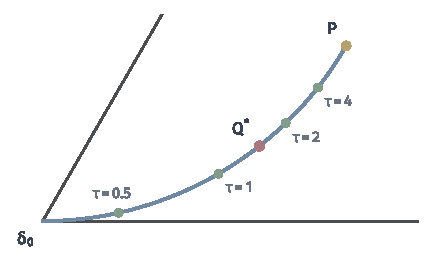
\includegraphics[width=72mm]{figures/07-probability/07-distribution-optimization/matplotlib/dsel-gibbs-path/figure.pdf}
 \caption{$\tau$从$0$增大到$\infty$时，$Q^{*}_\tau\propto P\,\mathrm{e}^{-V/\tau}$在概率三角形左下部分走过的路径（蓝），$P$均匀，$V(x)=x$。绿点依次是$\tau=0.5,1,2,4$，红点是$\tau=1/\ln2$时的$(\frac47,\frac27,\frac17)$，黄点是$P$。}
 \label{fig:dsel-gibbs-path}
\end{BookInlineFigure}

换一个角度看这个权衡。每个候选$Q$对应平面上的一点，横坐标是偏离$D_{\mathrm{KL}}(Q\Vert P)$，纵坐标是期望成本$\mathbb{E}_{Q}[V]$。目标$J_\tau$的等值线是斜率为$-\tau$的直线
\[
 \mathbb{E}_{Q}[V]=c-\tau D_{\mathrm{KL}}(Q\Vert P) .
\]
最小化$J_\tau$，就是把这条直线向下平移，直到它刚好碰到所有候选点组成的区域。图~\ref{fig:dsel-tradeoff}中，碰到的点正是$Q^{*}$；不同的$\tau$给出不同的斜率，碰到区域下边界上不同的点，而整条下边界就是上面那条Gibbs路径。下面的定理会证明这一点。

\begin{BookInlineFigure}
 \centering
 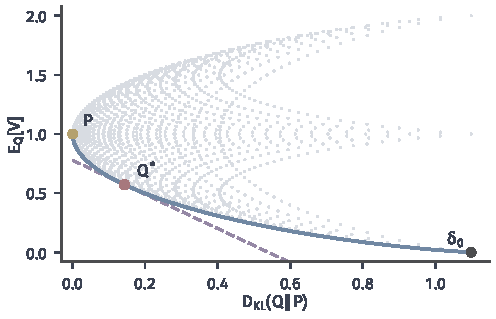
\includegraphics[width=84mm]{figures/07-probability/07-distribution-optimization/matplotlib/dsel-tradeoff/figure.pdf}
 \caption{成本与偏离的权衡，$P$均匀，$V(x)=x$。浅灰点是概率三角形中步长$1/60$的格点分布对应的$\bigl(D_{\mathrm{KL}}(Q\Vert P),\mathbb{E}_{Q}[V]\bigr)$；蓝线是Gibbs路径，它是可达区域的下边界。紫色虚线是$\tau=1/\ln2$时目标的等值线$\mathbb{E}_{Q}[V]=J^{*}-\tau D_{\mathrm{KL}}(Q\Vert P)$，在红点$Q^{*}$处与边界相切。}
 \label{fig:dsel-tradeoff}
\end{BookInlineFigure}

\paragraph{Gibbs分布的最优性}
有限状态上的形式推导提示了一般的答案：把$P$按$\mathrm{e}^{-V/\tau}$重新加权。下面在一般可测空间上定义它，并直接证明它的最优性。

\begin{definition}[Gibbs分布]
\label{def:dsel-gibbs}
设$P\in\mathcal{P}(\mathcal{X})$，$V:\mathcal{X}\to\mathbb{R}$可测，$\tau>0$，且
\begin{equation}
 Z=\mathbb{E}_{P}\bigl[\mathrm{e}^{-V/\tau}\bigr]<\infty .
 \label{eq:dsel-gibbs-partition}
\end{equation}
以
\begin{equation}
 \frac{\mathrm{d}Q^{*}_\tau}{\mathrm{d}P}=\frac{\mathrm{e}^{-V/\tau}}{Z}
 \label{eq:dsel-gibbs}
\end{equation}
定义的概率测度$Q^{*}_\tau$称为成本$V$、参数$\tau$相对于$P$的\term{Gibbs分布}（Gibbs distribution）。
\end{definition}

被积函数$\mathrm{e}^{-V/\tau}$处处为正，所以$Z>0$总成立，式~\eqref{eq:dsel-gibbs-partition}中真正的条件是$Z$有限。密度$\mathrm{e}^{-V/\tau}/Z$处处为正且有限，因此$Q^{*}_\tau$与$P$互相绝对连续：二者的零概率事件完全相同。

\begin{theorem}[Gibbs变分原理]
\label{thm:dsel-gibbs-variational}
设$V:\mathcal{X}\to\mathbb{R}$可测，$\tau>0$，$Z=\mathbb{E}_{P}[\mathrm{e}^{-V/\tau}]<\infty$，$Q^{*}=Q^{*}_\tau$为式~\eqref{eq:dsel-gibbs}的Gibbs分布。
\begin{enumerate}
 \item 对每个$Q\in\mathcal{Q}_V$，
 \begin{equation}
 J_\tau(Q)=-\tau\ln Z+\tau D_{\mathrm{KL}}(Q\Vert Q^{*}) .
 \label{eq:dsel-gibbs-identity}
 \end{equation}
 特别地，$J_\tau(Q)\geq-\tau\ln Z$。
 \item 若还有$\mathbb{E}_{Q^{*}}\lvert V\rvert<\infty$，则$Q^{*}\in\mathcal{Q}_V$，$J_\tau(Q^{*})=-\tau\ln Z$，并且$Q^{*}$是问题~\eqref{eq:dsel-kl-cost-problem}的唯一最优分布。
\end{enumerate}
\end{theorem}

\begin{proof}
第一部分。设$Q\in\mathcal{Q}_V$。由$D_{\mathrm{KL}}(Q\Vert P)<\infty$知$Q\ll P$；$P$与$Q^{*}$互相绝对连续，所以$Q\ll Q^{*}$。由密度的链式法则与式~\eqref{eq:dsel-gibbs}，$Q$几乎处处有
\[
 \frac{\mathrm{d}Q}{\mathrm{d}Q^{*}}=\frac{\mathrm{d}Q}{\mathrm{d}P}\cdot\frac{\mathrm{d}P}{\mathrm{d}Q^{*}}=\frac{\mathrm{d}Q}{\mathrm{d}P}\cdot Z\,\mathrm{e}^{V/\tau} .
\]
取对数，
\[
 \ln\frac{\mathrm{d}Q}{\mathrm{d}Q^{*}}=\ln\frac{\mathrm{d}Q}{\mathrm{d}P}+\frac{V}{\tau}+\ln Z .
\]

右边每一项都在$Q$下可积：$D_{\mathrm{KL}}(Q\Vert P)$有限，而对数比的负部总是可积的，所以$\ln(\mathrm{d}Q/\mathrm{d}P)$在$Q$下可积；$V$在$Q$下可积是$\mathcal{Q}_V$的定义；$\ln Z$是常数。于是可以对右边逐项取$Q$下的期望，左边的期望就是$D_{\mathrm{KL}}(Q\Vert Q^{*})$：
\[
 D_{\mathrm{KL}}(Q\Vert Q^{*})=D_{\mathrm{KL}}(Q\Vert P)+\frac{1}{\tau}\mathbb{E}_{Q}[V]+\ln Z .
\]
两边乘以$\tau$并移项，即得式~\eqref{eq:dsel-gibbs-identity}。由Gibbs不等式$D_{\mathrm{KL}}(Q\Vert Q^{*})\geq0$，得到$J_\tau(Q)\geq-\tau\ln Z$。

第二部分。由式~\eqref{eq:dsel-gibbs}，$\ln(\mathrm{d}Q^{*}/\mathrm{d}P)=-V/\tau-\ln Z$。当$V$在$Q^{*}$下可积时，它在$Q^{*}$下可积，
\[
 D_{\mathrm{KL}}(Q^{*}\Vert P)=-\frac1\tau\mathbb{E}_{Q^{*}}[V]-\ln Z<\infty ,
\]
所以$Q^{*}\in\mathcal{Q}_V$。在式~\eqref{eq:dsel-gibbs-identity}中取$Q=Q^{*}$，得到$J_\tau(Q^{*})=-\tau\ln Z$，它等于第一部分给出的下界，所以$Q^{*}$最优。若另一个$Q\in\mathcal{Q}_V$也达到这个值，则$D_{\mathrm{KL}}(Q\Vert Q^{*})=0$，由Gibbs不等式的等号条件$Q=Q^{*}$。
\end{proof}

定理~\ref{thm:dsel-gibbs-variational}称为\term{Gibbs变分原理}（Gibbs variational principle）。式~\eqref{eq:dsel-gibbs-identity}比“$Q^{*}$最优”说得更多：任何候选的目标值比最优值多出的部分，恰好是$\tau D_{\mathrm{KL}}(Q\Vert Q^{*})$。在例子中，$J_\tau(P)-J_\tau(Q^{*})\approx1-0.7776=0.2224$，而直接计算
\[
 \tau D_{\mathrm{KL}}(P\Vert Q^{*})=\frac{1}{3\ln2}\ln\Bigl(\frac{7}{12}\cdot\frac76\cdot\frac73\Bigr)=\frac13\log_2\frac{343}{216}\approx0.2224 ,
\]
两者一致。这个恒等式把“离最优还差多少”变成一个可以计算的散度，第~\ref{sec:dsel-checks}节将用它检验数值解。

最优值$-\tau\ln\mathbb{E}_{P}[\mathrm{e}^{-V/\tau}]$也有清楚的含义。令$g=-V/\tau$，第一部分可以改写为：对每个$Q\in\mathcal{Q}_V$，
\begin{equation}
 \mathbb{E}_{Q}[g]\leq D_{\mathrm{KL}}(Q\Vert P)+\ln\mathbb{E}_{P}\bigl[\mathrm{e}^{g}\bigr] ,
 \label{eq:dsel-dv}
\end{equation}
第~\ref{chap:distribution-comparison}章用这个不等式由KL散度控制期望差。定理的第二部分说明它不能再改进：当$\mathbb{E}_{Q^{*}}\lvert g\rvert<\infty$时，等号在指数倾斜$Q^{*}$处取到，于是
\[
 \ln\mathbb{E}_{P}\bigl[\mathrm{e}^{g}\bigr]=\max_{Q\in\mathcal{Q}_V}\Bigl\{\mathbb{E}_{Q}[g]-D_{\mathrm{KL}}(Q\Vert P)\Bigr\} .
\]
对数矩母函数是“期望减去偏离代价”在全体候选上的最大值。

Gibbs分布的形式不是事先选定的分布族，而是由目标推出来的。它是$P$沿统计量$V$、以参数$-1/\tau$作的指数倾斜，属于第~\ref{chap:distribution-families}章以$P$为基准测度、以$V$为自然统计量的指数族。

由定理还可以读出图~\ref{fig:dsel-tradeoff}中的下边界。设$Q\in\mathcal{Q}_V$的偏离不超过$Q^{*}$的偏离，即
\[
 D_{\mathrm{KL}}(Q\Vert P)\leq D_{\mathrm{KL}}(Q^{*}\Vert P) .
\]
由$J_\tau(Q)\geq J_\tau(Q^{*})$，
\[
 \begin{aligned}
 \mathbb{E}_{Q}[V]&\geq\mathbb{E}_{Q^{*}}[V]+\tau\bigl(D_{\mathrm{KL}}(Q^{*}\Vert P)-D_{\mathrm{KL}}(Q\Vert P)\bigr)\\
 &\geq\mathbb{E}_{Q^{*}}[V] .
 \end{aligned}
\]
也就是说，在不超过$Q^{*}$的偏离预算下，没有哪个分布的期望成本更低。

\paragraph{配分函数无穷时}
条件$Z<\infty$不是技术细节。回到第~\ref{sec:dsel-problems}节的可数例子：$P(k)=2^{-k}$，$V(k)=-k$，$k\geq1$。记$r=\mathrm{e}^{1/\tau}/2$，则
\[
 Z(\tau)=\sum_{k\geq1}2^{-k}\mathrm{e}^{k/\tau}=\sum_{k\geq1}r^{k} .
\]
它有限当且仅当$r<1$，即$\tau>1/\ln2$；这时$Z=r/(1-r)$，Gibbs分布$Q^{*}(k)=(1-r)r^{k-1}$是几何分布，$\mathbb{E}_{Q^{*}}\lvert V\rvert=1/(1-r)$有限，定理~\ref{thm:dsel-gibbs-variational}的两部分都适用。例如$\tau=2$时，$r\approx0.8244$，$Z\approx4.693$，最优值$-2\ln Z\approx-3.092$。

$\tau\leq1/\ln2$时没有Gibbs分布，最优值是$-\infty$。取$Q_N$为$\{1,\dots,N\}$上的均匀分布，它的期望成本与KL散度分别是
\[
 \begin{gathered}
 \mathbb{E}_{Q_N}[V]=-\frac{N+1}{2},\\
 D_{\mathrm{KL}}(Q_N\Vert P)=\frac1N\sum_{k=1}^{N}\bigl(k\ln2-\ln N\bigr)=\frac{(N+1)\ln2}{2}-\ln N .
 \end{gathered}
\]
代入目标，
\[
 J_\tau(Q_N)=\frac{N+1}{2}\bigl(\tau\ln2-1\bigr)-\tau\ln N .
\]
$\tau\ln2\leq1$时第一项不为正，第二项趋于$-\infty$，所以$J_\tau(Q_N)\to-\infty$。远处状态带来的收益$k$增长得不比偏离的代价$\tau k\ln2$慢，把质量往远处推永远划算。图~\ref{fig:dsel-partition-threshold}画出这一转变。

\begin{BookInlineFigure}
 \centering
 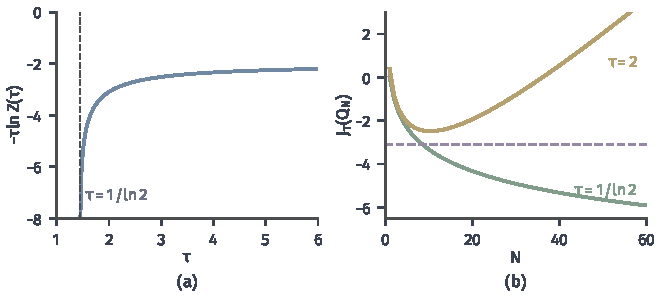
\includegraphics[width=112mm]{figures/07-probability/07-distribution-optimization/matplotlib/dsel-partition-threshold/figure.pdf}
 \caption{配分函数的有限性。$P(k)=2^{-k}$，$V(k)=-k$。(a)最优值$-\tau\ln Z(\tau)$（蓝），$\tau\downarrow1/\ln2$（深灰虚线）时趋于$-\infty$。(b)$\{1,\dots,N\}$上均匀分布$Q_N$的目标值：$\tau=1/\ln2$时（绿）等于$-\log_2N$，无下界；$\tau=2$时（黄）始终高于最优值$-2\ln Z(2)\approx-3.092$（紫色虚线）。}
 \label{fig:dsel-partition-threshold}
\end{BookInlineFigure}

定理第二部分的条件$\mathbb{E}_{Q^{*}}\lvert V\rvert<\infty$也可能不成立。那时$Z$有限，第一部分的恒等式仍然给出下界$-\tau\ln Z$，可是写出来的$Q^{*}$不在候选集合中。这种情形放到第~\ref{sec:dsel-checks}节，与“最小值是否被达到”一起讨论。


\section{矩约束下的最小KL}
\label{sec:dsel-min-kl}

上一节的成本是“软”的：成本可以高一点，只要偏离小一点。另一类要求是“硬”的：选出的分布必须满足某些平均量，例如平均点数必须是$10/7$。满足要求的分布在图~\ref{fig:dsel-three-requirements}中排成一条线段，我们要在这条线段上挑出离参考分布最近的一个。

设$\bm{T}:\mathcal{X}\to\mathbb{R}^{k}$可测，$\bm{m}\in\mathbb{R}^{k}$。满足矩要求的分布组成集合
\[
 \mathcal{C}_{\bm{m}}=\Bigl\{Q\in\mathcal{P}(\mathcal{X}):\ \mathbb{E}_{Q}\lVert\bm{T}\rVert_2<\infty,\ \mathbb{E}_{Q}[\bm{T}]=\bm{m}\Bigr\}.
\]
本节研究
\begin{equation}
 \min_{Q\in\mathcal{C}_{\bm{m}}}\ D_{\mathrm{KL}}(Q\Vert P) .
 \label{eq:dsel-min-kl-problem}
\end{equation}
所有能由$P$的绝对连续分布实现的矩组成\term{可行矩集合}（set of feasible moments）
\[
 \mathcal{M}=\Bigl\{\mathbb{E}_{Q}[\bm{T}]:\ Q\ll P,\ \mathbb{E}_{Q}\lVert\bm{T}\rVert_2<\infty\Bigr\}.
\]
只有$\bm{m}\in\mathcal{M}$时问题~\eqref{eq:dsel-min-kl-problem}才有KL有限的候选。

KL的方向在这里是$D_{\mathrm{KL}}(Q\Vert P)$：期望按待选的$Q$计算，有限的前提是$Q\ll P$。所以选出的分布可以删去$P$的某些状态，却不会在$P$认为不可能的地方放质量。参考分布代表原有的认识，矩要求是新加的条件，问题问的是：为了满足新条件，最少要把原有认识改动多少。若反过来最小化$D_{\mathrm{KL}}(P\Vert Q)$，期望按$P$计算，要求$Q$覆盖$P$的全部状态，这对应另一类问题，在第~\ref{chap:distribution-approximation}章讨论。

\subsection{指数倾斜}
\label{sec:dsel-tilt}

先在有限状态上求解。设$\mathcal{X}$有限，$p(x)>0$对每个$x$成立。这时每个$Q$都绝对连续于$P$，$Q$的矩是$\bm{T}(x)$的凸组合，而任何凸组合也都能由某个$Q$实现，所以
\[
 \mathcal{M}=\operatorname{conv}\{\bm{T}(x):x\in\mathcal{X}\}
\]
是有限个点的凸包。在例子中$T(x)=x$，$\mathcal{M}=[0,2]$。

\paragraph{乘子方程}
在概率三角形内部形式地求驻点。对归一化引入乘子$\nu$，对矩约束引入乘子向量$\bm{\theta}\in\mathbb{R}^{k}$，Lagrange函数为
\[
 \sum_xq(x)\ln\frac{q(x)}{p(x)}-\Bigl\langle\bm{\theta},\sum_xq(x)\bm{T}(x)-\bm{m}\Bigr\rangle-\nu\Bigl(\sum_xq(x)-1\Bigr).
\]
对$q(x)$求偏导并令其为零，得到
\[
 \ln\frac{q(x)}{p(x)}+1-\langle\bm{\theta},\bm{T}(x)\rangle-\nu=0 .
\]

解出
\[
 q(x)=p(x)\exp\bigl(\langle\bm{\theta},\bm{T}(x)\rangle\bigr)\,\mathrm{e}^{\nu-1} ,
\]
再由归一化定出常数因子：
\begin{equation}
 q_{\bm{\theta}}(x)=p(x)\exp\bigl(\langle\bm{\theta},\bm{T}(x)\rangle-A(\bm{\theta})\bigr),\qquad A(\bm{\theta})=\ln\sum_xp(x)\,\mathrm{e}^{\langle\bm{\theta},\bm{T}(x)\rangle} .
 \label{eq:dsel-tilt-finite}
\end{equation}
乘子$\bm{\theta}$还没有确定，它要使$q_{\bm{\theta}}$满足矩约束。Lagrange乘子法给出的是必要条件的形式（见\BookChapterRef{chap:constrained-optimality}{卷五第17章“约束问题的最优性”}），这里又假设了解在内部，所以式~\eqref{eq:dsel-tilt-finite}仍只是候选。

这个形式在一般空间上同样有意义。

\begin{definition}[指数倾斜]
\label{def:dsel-tilt}
设$P\in\mathcal{P}(\mathcal{X})$，$\bm{\theta}\in\mathbb{R}^{k}$，并且
\begin{equation}
 A(\bm{\theta})=\ln\mathbb{E}_{P}\bigl[\mathrm{e}^{\langle\bm{\theta},\bm{T}\rangle}\bigr]<\infty .
 \label{eq:dsel-tilt-partition}
\end{equation}
以
\begin{equation}
 \frac{\mathrm{d}Q_{\bm{\theta}}}{\mathrm{d}P}=\exp\bigl(\langle\bm{\theta},\bm{T}\rangle-A(\bm{\theta})\bigr)
 \label{eq:dsel-tilt}
\end{equation}
定义的$Q_{\bm{\theta}}$称为$P$沿$\bm{T}$的\term{指数倾斜}（exponential tilting）。
\end{definition}

全体$Q_{\bm{\theta}}$就是第~\ref{chap:distribution-families}章以$P$为基准测度、以$\bm{T}$为自然统计量的指数族，$A$是它的对数配分函数。密度处处为正，所以每个$Q_{\bm{\theta}}$与$P$互相绝对连续。在例子中，$P$均匀，$T(x)=x$，$q_\theta(x)\propto\mathrm{e}^{\theta x}$。取$\theta=\ln2$，三个权重是$1,2,4$，
\[
 Q_{\ln2}=\Bigl(\frac17,\ \frac27,\ \frac47\Bigr),\qquad\mathbb{E}_{Q_{\ln2}}[X]=\frac{2+8}{7}=\frac{10}{7},
\]
它恰好落在约束线段上。

\paragraph{勾股恒等式}
要说明$Q_{\ln2}$比线段上其他分布更接近$P$，不必求导，只需把$D_{\mathrm{KL}}(Q\Vert P)$拆开，得到下面的\term{勾股恒等式}。

\begin{lemma}[勾股恒等式]
\label{lem:dsel-pythagoras}
设$A(\bm{\theta})<\infty$，$Q\in\mathcal{C}_{\bm{m}}$且$D_{\mathrm{KL}}(Q\Vert P)<\infty$。则
\begin{equation}
 D_{\mathrm{KL}}(Q\Vert P)=D_{\mathrm{KL}}(Q\Vert Q_{\bm{\theta}})+\langle\bm{\theta},\bm{m}\rangle-A(\bm{\theta}) .
 \label{eq:dsel-pythagoras-general}
\end{equation}
若$Q_{\bm{\theta}}$本身也属于$\mathcal{C}_{\bm{m}}$，则
\begin{equation}
 D_{\mathrm{KL}}(Q\Vert P)=D_{\mathrm{KL}}(Q\Vert Q_{\bm{\theta}})+D_{\mathrm{KL}}(Q_{\bm{\theta}}\Vert P) .
 \label{eq:dsel-pythagoras}
\end{equation}
\end{lemma}

\begin{proof}
$Q\ll P$，而$P$与$Q_{\bm{\theta}}$互相绝对连续，所以$Q\ll Q_{\bm{\theta}}$。由链式法则与式~\eqref{eq:dsel-tilt}，
\[
 \ln\frac{\mathrm{d}Q}{\mathrm{d}Q_{\bm{\theta}}}=\ln\frac{\mathrm{d}Q}{\mathrm{d}P}-\langle\bm{\theta},\bm{T}\rangle+A(\bm{\theta}) .
\]
右边第一项在$Q$下可积（KL有限，负部总可积），第二项因$\mathbb{E}_{Q}\lVert\bm{T}\rVert_2<\infty$可积。逐项取$Q$下的期望，并用$\mathbb{E}_{Q}[\bm{T}]=\bm{m}$，
\[
 D_{\mathrm{KL}}(Q\Vert Q_{\bm{\theta}})=D_{\mathrm{KL}}(Q\Vert P)-\langle\bm{\theta},\bm{m}\rangle+A(\bm{\theta}) ,
\]
移项即得式~\eqref{eq:dsel-pythagoras-general}。若$Q_{\bm{\theta}}\in\mathcal{C}_{\bm{m}}$，则式~\eqref{eq:dsel-tilt}给出的对数密度在$Q_{\bm{\theta}}$下可积，其期望是
\[
 D_{\mathrm{KL}}(Q_{\bm{\theta}}\Vert P)=\langle\bm{\theta},\bm{m}\rangle-A(\bm{\theta}) .
\]
代回式~\eqref{eq:dsel-pythagoras-general}即得式~\eqref{eq:dsel-pythagoras}。
\end{proof}

证明的关键一步是：$\ln(\mathrm{d}Q_{\bm{\theta}}/\mathrm{d}P)$只通过$\bm{T}$依赖于$x$，而约束集合中所有分布的$\bm{T}$平均值都相同，所以这个对数比在约束集合上的平均是常数。

在例子中验证。取线段的一个端点$Q=(\tfrac27,0,\tfrac57)$，三个散度分别是
\[
 \begin{gathered}
 D_{\mathrm{KL}}(Q\Vert P)=\tfrac27\ln\tfrac67+\tfrac57\ln\tfrac{15}7\approx0.5003,\\
 D_{\mathrm{KL}}(Q\Vert Q_{\ln2})=\tfrac27\ln2+\tfrac57\ln\tfrac54\approx0.3574,\qquad D_{\mathrm{KL}}(Q_{\ln2}\Vert P)\approx0.1429 .
 \end{gathered}
\]
后两项之和正是第一项。图~\ref{fig:dsel-pythagoras}把这三个量画成一个“直角三角形”：约束集合是一条直线，倾斜族是与它相交的曲线，交点$Q_{\ln2}$像是垂足。

\begin{BookInlineFigure}
 \centering
 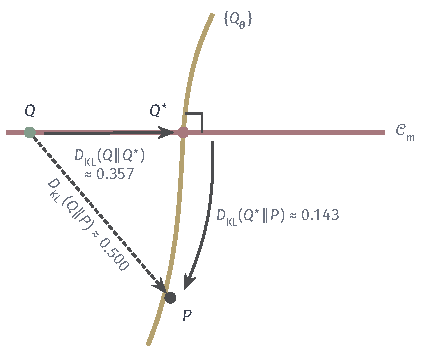
\includegraphics[width=72mm]{figures/07-probability/07-distribution-optimization/tikz/dsel-pythagoras/figure.pdf}
 \caption{勾股恒等式的示意。红线是约束集合$\mathcal{C}_{\bm{m}}$，黄线是倾斜族$\{Q_{\bm{\theta}}\}$，两者交于$Q^{*}=Q_{\ln2}$。箭头从KL的第一个分布指向第二个分布，数值取自$P$均匀、$T(x)=x$、$m=10/7$、$Q=(\frac27,0,\frac57)$的例子，单位为nat。}
 \label{fig:dsel-pythagoras}
\end{BookInlineFigure}

这个“勾股”只是类比。KL散度不对称，也不满足三角不等式，恒等式~\eqref{eq:dsel-pythagoras}只在一个点位于约束集合、另一个点是满足同一约束的倾斜分布时成立。三角形中实际的几何如图~\ref{fig:dsel-kl-projection}：以$P$为中心的KL等值线一圈圈向外扩张，第一次碰到约束线段的地方就是$Q_{\ln2}$，倾斜族的曲线恰好从这一点穿过。

\begin{BookInlineFigure}
 \centering
 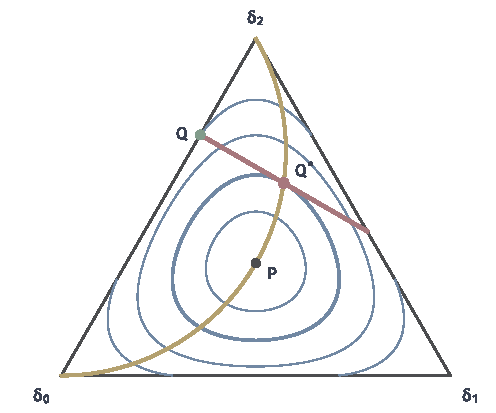
\includegraphics[width=84mm]{figures/07-probability/07-distribution-optimization/matplotlib/dsel-kl-projection/figure.pdf}
 \caption{约束线段上离$P$最近的分布。蓝线是$D_{\mathrm{KL}}(Q\Vert P)$的等值线，取值$0.05,0.3,0.5$（细）与最小值$D^{*}\approx0.1429$（粗）；红色线段是$\mathbb{E}_{Q}[X]=10/7$；黄线是倾斜族$q_\theta\propto\mathrm{e}^{\theta x}$。粗等值线在红点$Q^{*}=(\frac17,\frac27,\frac47)$处与线段相切；绿点$Q=(\frac27,0,\frac57)$满足约束，但落在更外圈。}
 \label{fig:dsel-kl-projection}
\end{BookInlineFigure}

\paragraph{最优性与存在性}
引理把最优性归结为一件事：能否找到$\bm{\theta}$，使$Q_{\bm{\theta}}$满足约束。这需要$\bm{m}$离可行矩集合的边界有一段距离。可行矩集合可能是低维的，例如当所有$\bm{T}(x)$都落在$\mathbb{R}^{2}$的一条直线上时，$\mathcal{M}$是一条线段，它在平面中没有内点。所以“远离边界”要在$\mathcal{M}$所在的仿射包$\operatorname{aff}\mathcal{M}$内衡量：$\bm{m}$属于$\mathcal{M}$的相对内部$\operatorname{ri}\mathcal{M}$，是指存在$\varepsilon>0$，使$\operatorname{aff}\mathcal{M}$中与$\bm{m}$距离小于$\varepsilon$的点都在$\mathcal{M}$中。上面的线段，相对内部就是去掉两个端点。

\begin{theorem}[指数倾斜给出最小KL]
\label{thm:dsel-min-kl}
设$\mathcal{X}$有限，$p(x)>0$对每个$x$成立，$\bm{m}\in\operatorname{ri}\mathcal{M}$。则
\begin{enumerate}
 \item 存在$\bm{\theta}^{*}\in\mathbb{R}^{k}$，使$\mathbb{E}_{Q_{\bm{\theta}^{*}}}[\bm{T}]=\bm{m}$；
 \item $Q^{*}=Q_{\bm{\theta}^{*}}$是问题~\eqref{eq:dsel-min-kl-problem}的唯一最优分布，最优值为
 \begin{equation}
 D^{*}=\langle\bm{\theta}^{*},\bm{m}\rangle-A(\bm{\theta}^{*}) ;
 \label{eq:dsel-min-kl-value}
 \end{equation}
 \item 满足第一条的$\bm{\theta}^{*}$可能不唯一，但它们给出同一个$Q^{*}$。
\end{enumerate}
\end{theorem}

\begin{proof}
第一部分。令
\[
 \ell(\bm{\theta})=\langle\bm{\theta},\bm{m}\rangle-A(\bm{\theta}) ,
\]
我们证明它有最大值点，并且最大值点满足矩约束。把$\ell$写成
\[
 -\ell(\bm{\theta})=\ln\sum_xp(x)\,\mathrm{e}^{\langle\bm{\theta},\bm{T}(x)-\bm{m}\rangle} .
\]
记
\[
 L=\operatorname{span}\{\bm{T}(x)-\bm{m}:x\in\mathcal{X}\} .
\]
因为$\bm{m}\in\mathcal{M}$，有$\operatorname{aff}\mathcal{M}=\bm{m}+L$。若$\bm{a}\perp L$，则每个指数中$\langle\bm{a},\bm{T}(x)-\bm{m}\rangle=0$，所以$\ell(\bm{\theta}+\bm{a})=\ell(\bm{\theta})$。只需在子空间$L$上找最大值点。

对$L$中的单位向量$\bm{u}$，令
\[
 \delta(\bm{u})=\max_{x\in\mathcal{X}}\langle\bm{u},\bm{T}(x)-\bm{m}\rangle .
\]
由于$\bm{m}\in\operatorname{ri}\mathcal{M}$，存在$\varepsilon>0$使$\bm{m}+\varepsilon\bm{u}\in\mathcal{M}$，即它是某个凸组合$\sum_xq(x)\bm{T}(x)$。与$\bm{u}$作内积，
\[
 \varepsilon=\sum_xq(x)\langle\bm{u},\bm{T}(x)-\bm{m}\rangle\leq\delta(\bm{u}) .
\]
所以$\delta(\bm{u})>0$。$\delta$在$L$的单位球面上连续，球面紧，于是$\delta_0=\min\delta(\bm{u})>0$。

对$\bm{\theta}\in L$，$\bm{\theta}\neq\bm{0}$，取$\bm{u}=\bm{\theta}/\lVert\bm{\theta}\rVert_2$。和式中至少有一项的指数是$\lVert\bm{\theta}\rVert_2\,\delta(\bm{u})$，其余各项为正，记$p_{\min}=\min_xp(x)>0$，得到
\[
 -\ell(\bm{\theta})\geq\ln p_{\min}+\delta_0\lVert\bm{\theta}\rVert_2 .
\]
所以$-\ell$在$L$上连续且当$\lVert\bm{\theta}\rVert_2\to\infty$时趋于$+\infty$，它在$L$的某个闭球上取到在$L$上的最小值，设最小值点为$\bm{\theta}^{*}$。由$\ell$沿$L^{\perp}$不变，$\bm{\theta}^{*}$也是$\ell$在整个$\mathbb{R}^{k}$上的最大值点。

$\ell$可微，最大值点处梯度为零。对式~\eqref{eq:dsel-tilt-finite}中的$A$求梯度，
\[
 \nabla A(\bm{\theta})=\frac{\sum_xp(x)\bm{T}(x)\mathrm{e}^{\langle\bm{\theta},\bm{T}(x)\rangle}}{\sum_xp(x)\mathrm{e}^{\langle\bm{\theta},\bm{T}(x)\rangle}}=\mathbb{E}_{Q_{\bm{\theta}}}[\bm{T}] .
\]
于是
\[
 \nabla\ell(\bm{\theta}^{*})=\bm{m}-\mathbb{E}_{Q_{\bm{\theta}^{*}}}[\bm{T}]=\bm{0} .
\]


第二部分。有限状态上每个$Q\in\mathcal{C}_{\bm{m}}$都满足$D_{\mathrm{KL}}(Q\Vert P)<\infty$。由引理~\ref{lem:dsel-pythagoras}，
\[
 D_{\mathrm{KL}}(Q\Vert P)=D_{\mathrm{KL}}(Q\Vert Q^{*})+D_{\mathrm{KL}}(Q^{*}\Vert P)\geq D_{\mathrm{KL}}(Q^{*}\Vert P),
\]
等号当且仅当$D_{\mathrm{KL}}(Q\Vert Q^{*})=0$，即$Q=Q^{*}$。最优值由引理中的表达式给出。

第三部分。若$\bm{\theta}^{*}$与$\bm{\theta}'$都满足矩约束，则$Q_{\bm{\theta}^{*}}$与$Q_{\bm{\theta}'}$都是最优分布，由唯一性二者相同。
\end{proof}

三个条件各有作用。$p(x)>0$保证每个候选都绝对连续于$P$；若$P$有零概率的状态，先把它们从$\mathcal{X}$中删去即可。有限性保证$A(\bm{\theta})$对一切$\bm{\theta}$有限，也提供了证明中的紧性。$\bm{m}\in\operatorname{ri}\mathcal{M}$保证存在有限的$\bm{\theta}^{*}$；第~\ref{sec:dsel-moment-matching}节会看到，$\bm{m}$在边界上时最优分布仍然存在，但不再是任何$Q_{\bm{\theta}}$。

在例子中，$\theta^{*}=\ln2$，$A(\ln2)=\ln\frac{1+2+4}{3}=\ln\frac73$，由式~\eqref{eq:dsel-min-kl-value}，
\[
 D^{*}=\frac{10}{7}\ln2-\ln\frac73\approx0.9902-0.8473=0.1429 ,
\]
与直接计算一致。

\paragraph{指数族从哪里来}
问题~\eqref{eq:dsel-min-kl-problem}的候选是$\mathcal{X}$上的全部分布，并没有限定在某个参数族中，最优解却落在以$P$为基准、以约束统计量$\bm{T}$为自然统计量的指数族里。Lagrange乘子变成了自然参数，要约束哪些平均量，就决定了用哪些统计量作指数权重。所以这一步不能理解为“先选一个指数族，再在族内近似”：族是最优性条件的产物。第~\ref{chap:distribution-approximation}章研究的是另一类问题，那里先限定候选族，再在族内逼近一个给定的目标分布。

上一节的Gibbs分布也是这样的解。取$\bm{T}=V$，$\bm{\theta}=-1/\tau$，Gibbs分布$Q^{*}_\tau$就是$P$沿$V$的倾斜；由定理~\ref{thm:dsel-min-kl}，它是所有满足$\mathbb{E}_{Q}[V]=\mathbb{E}_{Q^{*}_\tau}[V]$的分布中离$P$最近的一个。例如$(\tfrac47,\tfrac27,\tfrac17)$是平均成本为$4/7$的分布中KL最小者。成本加罚的软约束与矩的硬约束，在指数倾斜这里汇合。

\subsection{矩匹配}
\label{sec:dsel-moment-matching}

定理~\ref{thm:dsel-min-kl}把“选一个分布”变成了“解一个方程”：找$\bm{\theta}$使
\begin{equation}
 \nabla A(\bm{\theta})=\mathbb{E}_{Q_{\bm{\theta}}}[\bm{T}]=\bm{m} .
 \label{eq:dsel-moment-matching}
\end{equation}
这称为\term{矩匹配方程}（moment-matching equation）。未知数只有$k$个，与$\mathcal{X}$的大小无关。第~\ref{chap:distribution-families}章已经知道，在自然参数域内部$\nabla A$是均值映射，$A$的Hessian是统计量的协方差矩阵：
\[
 \nabla^{2}A(\bm{\theta})=\operatorname{Cov}_{Q_{\bm{\theta}}}(\bm{T}) .
\]
本小节用这两个事实分析方程的求解、冗余统计量的影响和边界上的矩。

\paragraph{对偶函数}
式~\eqref{eq:dsel-pythagoras-general}还给出一个与$\bm{\theta}$是否满足约束无关的不等式。由$D_{\mathrm{KL}}(Q\Vert Q_{\bm{\theta}})\geq0$，对每个$Q\in\mathcal{C}_{\bm{m}}$与每个使$A(\bm{\theta})$有限的$\bm{\theta}$，
\begin{equation}
 D_{\mathrm{KL}}(Q\Vert P)\geq\ell(\bm{\theta})=\langle\bm{\theta},\bm{m}\rangle-A(\bm{\theta}) .
 \label{eq:dsel-weak-duality}
\end{equation}
这个不等式不要求$\mathcal{X}$有限。每个$\bm{\theta}$给出最优值的一个下界，每个可行的$Q$给出一个上界。$\ell$称为对偶函数，它是凹函数，因为$A$是凸函数。

方程~\eqref{eq:dsel-moment-matching}正是$\nabla\ell(\bm{\theta})=\bm{0}$，即$\bm{\theta}$是$\ell$的最大值点。在定理~\ref{thm:dsel-min-kl}的条件下，上下界在这里相遇：
\[
 \max_{\bm{\theta}}\ell(\bm{\theta})=\min_{Q\in\mathcal{C}_{\bm{m}}}D_{\mathrm{KL}}(Q\Vert P) .
\]
这就是Lagrange对偶，下界~\eqref{eq:dsel-weak-duality}是弱对偶，等号是强对偶（一般理论见\BookChapterRef{chap:duality}{卷五第18章“对偶问题”}）。$k$维的凹函数最大化比在全体分布上的最小化容易得多，这是实际求解时总是转到$\bm{\theta}$上的原因。

图~\ref{fig:dsel-dual-function}画出例子中的$-\ell(\theta)=A(\theta)-\theta m$。$m=1$时最小值点是$\theta=0$，因为$P$本身已满足约束，$D^{*}=0$。$m=10/7$时最小值点是$\ln2$，最小值$-D^{*}\approx-0.1429$。$m=2$在可行矩集合$[0,2]$的端点，曲线单调下降，趋于$-\ln3$而达不到：上界与下界仍相等，因为唯一可行的分布$\delta_2$满足$D_{\mathrm{KL}}(\delta_2\Vert P)=\ln3$，但没有有限的$\theta$达到它。

\begin{BookInlineFigure}
 \centering
 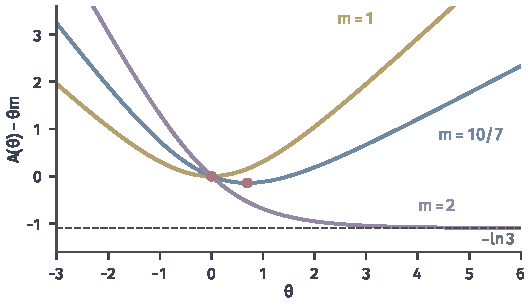
\includegraphics[width=90mm]{figures/07-probability/07-distribution-optimization/matplotlib/dsel-dual-function/figure.pdf}
 \caption{对偶函数取负号后的$A(\theta)-\theta m$，$A(\theta)=\ln\frac{1+\mathrm{e}^{\theta}+\mathrm{e}^{2\theta}}{3}$。黄：$m=1$，最小值$0$在$\theta=0$；蓝：$m=10/7$，最小值$-0.1429$在$\theta=\ln2$（红点）；紫：$m=2$，单调下降，下确界$-\ln3$（深灰虚线）不被达到。}
 \label{fig:dsel-dual-function}
\end{BookInlineFigure}

\paragraph{Hessian与局部求解}
对偶函数的Hessian是协方差矩阵的相反数。对任意$\bm{a}$，
\[
 \bm{a}^{\top}\operatorname{Cov}_{Q_{\bm{\theta}}}(\bm{T})\,\bm{a}=\operatorname{Var}_{Q_{\bm{\theta}}}\bigl(\langle\bm{a},\bm{T}\rangle\bigr)\geq0 ,
\]
等号当且仅当$\langle\bm{a},\bm{T}\rangle$在$Q_{\bm{\theta}}$下几乎必然为常数。有限状态、$p>0$时$Q_{\bm{\theta}}$处处为正，这就是$\langle\bm{a},\bm{T}(x)\rangle$对所有$x$相等。若不存在这样的$\bm{a}\neq\bm{0}$，即统计量之间没有仿射关系，则协方差矩阵对每个$\bm{\theta}$正定。

协方差正定时，$\bm{\theta}\mapsto\nabla A(\bm{\theta})$的Jacobian矩阵可逆，由反函数定理（见\BookChapterRef{chap:implicit-inverse-functions}{卷二第22章“隐函数与反函数”}），它的逆$\bm{m}\mapsto\bm{\theta}(\bm{m})$在$\operatorname{ri}\mathcal{M}$上光滑，导数是协方差矩阵的逆：
\[
 \frac{\partial\bm{\theta}}{\partial\bm{m}}=\operatorname{Cov}_{Q_{\bm{\theta}}}(\bm{T})^{-1} .
\]
在例子中$m=10/7$处$\operatorname{Var}_{Q_{\ln2}}(X)=26/49$，所以$\mathrm{d}\theta/\mathrm{d}m=49/26\approx1.885$：平均值再提高$0.01$，参数约需增加$0.019$。方差越小，同样的矩变化需要越大的参数变化；靠近可行矩集合的边界时方差趋于零，参数随之发散，这在后面的边界情形中会看到。

求解方程~\eqref{eq:dsel-moment-matching}的标准方法是Newton法：在当前点把$\nabla A$线性化，令线性化后的矩等于$\bm{m}$。迭代公式是
\begin{equation}
 \bm{\theta}^{(t+1)}=\bm{\theta}^{(t)}-\operatorname{Cov}_{Q_{\bm{\theta}^{(t)}}}(\bm{T})^{-1}\Bigl(\mathbb{E}_{Q_{\bm{\theta}^{(t)}}}[\bm{T}]-\bm{m}\Bigr).
 \label{eq:dsel-newton}
\end{equation}
它也是对凹函数$\ell$的Newton法（见\BookChapterRef{chap:second-order-methods}{卷五第7章“二阶方法”}）。每一步需要在当前倾斜分布下计算$\bm{T}$的均值与协方差。

在例子中从$\theta^{(0)}=0$出发。此时$Q$均匀，均值$1$，方差$2/3$，由式~\eqref{eq:dsel-newton}，
\[
 \theta^{(1)}=0-\frac{1-10/7}{2/3}=\frac{9}{14}\approx0.6429 .
\]
在$\theta^{(1)}$处，$Q\approx(0.1534,0.2917,0.5549)$，均值约$1.40147$，方差约$0.54708$，于是
\[
 \theta^{(2)}\approx0.6429-\frac{1.40147-1.42857}{0.54708}\approx0.692394 .
\]
再一步得到$\theta^{(3)}\approx0.6931470$，与$\ln2=0.69314718\ldots$相差约$2\times10^{-7}$。矩残差依次约为$0.43$、$2.7\times10^{-2}$、$4.0\times10^{-4}$、$9.4\times10^{-8}$，每步有效数字约翻倍，这是Newton法在解附近的二次收敛。

离解较远时，线性化可能越过头。图~\ref{fig:dsel-newton-steps}(a)从$\theta^{(0)}=-1$出发，第一步跳到$1.365$，越过了$\ln2$，第二步回到$0.451$，之后才进入二次收敛的范围。因为$\ell$是凹的，加上沿Newton方向的步长搜索即可保证从任意起点收敛；协方差接近奇异时，步长与方程的病态都要另作处理。

\begin{BookInlineFigure}
 \centering
 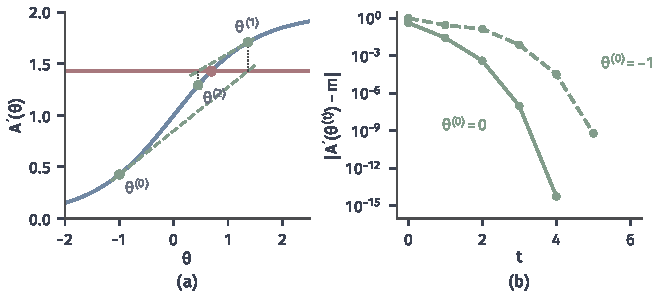
\includegraphics[width=112mm]{figures/07-probability/07-distribution-optimization/matplotlib/dsel-newton-steps/figure.pdf}
 \caption{用Newton法解矩匹配方程$A'(\theta)=10/7$。(a)均值映射$A'(\theta)$（蓝），目标水平$m=10/7$（红线），从$\theta^{(0)}=-1$出发的前两条切线（绿色虚线）与迭代点（绿）；红点是解$\theta=\ln2$。(b)矩残差$\lvert A'(\theta^{(t)})-m\rvert$，纵轴为对数刻度，实线从$\theta^{(0)}=0$出发，虚线从$\theta^{(0)}=-1$出发。}
 \label{fig:dsel-newton-steps}
\end{BookInlineFigure}

\paragraph{冗余统计量}
若统计量之间有仿射关系，协方差矩阵就奇异，Newton步中的线性方程不能唯一求解。取$\bm{T}(x)=(x,\,2-x)$，要求$\bm{m}=(\tfrac{10}7,\tfrac47)$。两个约束说的是同一件事，因为$T_1+T_2\equiv2$。倾斜分布为
\[
 q_{\bm{\theta}}(x)\propto\mathrm{e}^{\theta_1x+\theta_2(2-x)}=\mathrm{e}^{2\theta_2}\,\mathrm{e}^{(\theta_1-\theta_2)x},
\]
只依赖$\theta_1-\theta_2$。满足矩约束的$\bm{\theta}$组成整条直线$\theta_1-\theta_2=\ln2$，它们给出同一个$Q^{*}=(\tfrac17,\tfrac27,\tfrac47)$，正如定理~\ref{thm:dsel-min-kl}第三部分所说。记$v=\operatorname{Var}_{Q_{\bm{\theta}}}(X)$，协方差矩阵
\[
 \operatorname{Cov}_{Q_{\bm{\theta}}}(\bm{T})=v\begin{bmatrix}1&-1\\-1&1\end{bmatrix}
\]
沿$(1,1)$方向为零。图~\ref{fig:dsel-redundant}中，对偶函数的等值线都平行于$(1,1)$，最大值点不是一个点而是一条谷线。

\begin{BookInlineFigure}
 \centering
 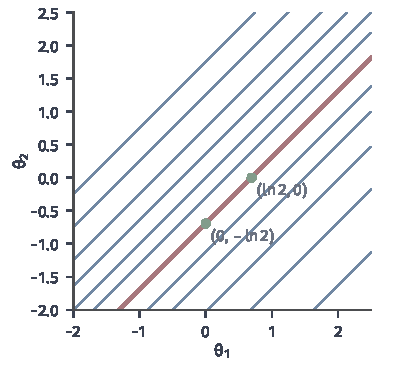
\includegraphics[width=70mm]{figures/07-probability/07-distribution-optimization/matplotlib/dsel-redundant/figure.pdf}
 \caption{冗余统计量$\bm{T}(x)=(x,2-x)$时的对偶函数，$P$均匀，$\bm{m}=(\frac{10}7,\frac47)$。蓝线是$A(\bm{\theta})-\langle\bm{\theta},\bm{m}\rangle$的等值线，全部平行于$(1,1)$；红线$\theta_1-\theta_2=\ln2$上每一点都是最优参数，绿点$(0,-\ln2)$与$(\ln2,0)$是其中两个，它们给出同一个分布。}
 \label{fig:dsel-redundant}
\end{BookInlineFigure}

处理办法有两种：删去多余的统计量，使表示成为第~\ref{chap:distribution-families}章的最小表示；或者保留冗余，在奇异的线性方程中取任意一个解，例如范数最小的解，最后得到的分布不受影响。冗余还带来一个必须先检查的问题：矩要求本身要相容。若要求$\bm{m}=(\tfrac{10}7,1)$，则$m_1+m_2\neq2$，$\bm{m}$不在$\operatorname{aff}\mathcal{M}$中，没有任何分布满足它；这时Newton迭代找不到解，问题出在约束而不在算法。

\paragraph{边界上的矩}
最后看$\bm{m}\in\mathcal{M}$但不在相对内部的情形。取$T(x)=\mathbf{1}_{\{x\geq1\}}$，$P$均匀，可行矩集合是$[0,1]$。对$0<m<1$，倾斜分布与矩约束为
\[
 Q_\theta=\frac{(1,\ \mathrm{e}^{\theta},\ \mathrm{e}^{\theta})}{1+2\mathrm{e}^{\theta}},\qquad\frac{2\mathrm{e}^{\theta}}{1+2\mathrm{e}^{\theta}}=m .
\]
解得$\theta(m)=\ln\dfrac{m}{2(1-m)}$，最优分布是$(1-m,\ \tfrac m2,\ \tfrac m2)$。

$m\to1$时$\theta(m)\to+\infty$。而$m=1$时可行的分布只有$(0,s,1-s)$，$0\leq s\leq1$，它们的KL是
\[
 D_{\mathrm{KL}}\bigl((0,s,1-s)\Vert P\bigr)=s\ln(3s)+(1-s)\ln\bigl(3(1-s)\bigr),
\]
在$s=\tfrac12$处最小，最优分布是$(0,\tfrac12,\tfrac12)$，最优值$\ln\tfrac32\approx0.4055$。它在状态$0$上的概率为零，不等于任何$Q_\theta$，却是$\theta\to\infty$时$Q_\theta$的极限。图~\ref{fig:dsel-boundary-face}画出参数的发散与最优值的连续：$D^{*}(m)$平稳地趋于$\ln\tfrac32$，$\theta(m)$却趋于无穷。

\begin{BookInlineFigure}
 \centering
 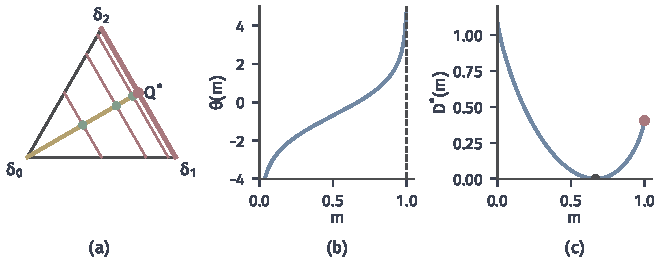
\includegraphics[width=112mm]{figures/07-probability/07-distribution-optimization/matplotlib/dsel-boundary-face/figure.pdf}
 \caption{边界上的矩，$T(x)=\mathbf{1}_{\{x\geq1\}}$，$P$均匀。(a)倾斜族是从$\delta_0$到$(0,\frac12,\frac12)$的线段（黄）；细红线是$m=0.5,0.8,0.95$的约束，绿点是各自的最优分布；粗红线是$m=1$时的可行集合，即$q(0)=0$的那条边，红点是最优分布。(b)参数$\theta(m)$，$m\to1$时发散。(c)最优值$D^{*}(m)$，在$m=2/3$处为零（$P$本身可行），在$m=1$处连续地达到$\ln\frac32$。}
 \label{fig:dsel-boundary-face}
\end{BookInlineFigure}

一般情形的结论如下。

\begin{theorem}[边界上的矩]
\label{thm:dsel-boundary}
设$\mathcal{X}$有限，$p(x)>0$对每个$x$成立，$\bm{m}\in\mathcal{M}\setminus\operatorname{ri}\mathcal{M}$。则
\begin{enumerate}
 \item 问题~\eqref{eq:dsel-min-kl-problem}有最优分布；
 \item 存在$\bm{a}\in\mathbb{R}^{k}$与$c\in\mathbb{R}$，使$\langle\bm{a},\bm{T}(x)\rangle\leq c$对一切$x$成立，$\langle\bm{a},\bm{m}\rangle=c$，且集合$F=\{x:\langle\bm{a},\bm{T}(x)\rangle=c\}$不是整个$\mathcal{X}$；每个$Q\in\mathcal{C}_{\bm{m}}$都满足$Q(F)=1$，因而没有任何$Q_{\bm{\theta}}$属于$\mathcal{C}_{\bm{m}}$；
 \item 对$Q(F)=1$的$Q$，记$P_F=P(\cdot\mid F)$，有
 \begin{equation}
 D_{\mathrm{KL}}(Q\Vert P)=D_{\mathrm{KL}}(Q\Vert P_F)-\ln P(F) ;
 \label{eq:dsel-face-reduction}
 \end{equation}
 \item 若$\bm{m}$属于$\operatorname{conv}\{\bm{T}(x):x\in F\}$的相对内部，则最优分布是$P_F$沿$\bm{T}$的倾斜$Q^{*}_F$，并且对满足$\mathbb{E}_{Q^{*}_F}[\bm{T}]=\bm{m}$的参数$\bm{\theta}_F$，$s\to+\infty$时$Q_{\bm{\theta}_F+s\bm{a}}\to Q^{*}_F$。
\end{enumerate}
\end{theorem}

\begin{proof}
第一部分。$\mathcal{C}_{\bm{m}}$由线性等式与非负性在概率单纯形中定出，是非空的有界闭集；$p>0$时$Q\mapsto\sum_xq(x)\ln(q(x)/p(x))$在单纯形上连续（约定$0\ln0=0$）。连续函数在非空紧集上取到最小值。

第二部分。$\mathcal{M}$是有限个点的凸包，$\bm{m}$在它的相对边界上。在仿射包$\operatorname{aff}\mathcal{M}$内对$\mathcal{M}$用凸集的支撑超平面定理，得到$\bm{a}\in L$（$L$是$\operatorname{aff}\mathcal{M}$的方向子空间）与$c$，使$\langle\bm{a},\bm{t}\rangle\leq c$对$\bm{t}\in\mathcal{M}$成立，$\langle\bm{a},\bm{m}\rangle=c$，且$\langle\bm{a},\cdot\rangle$在$\mathcal{M}$上不是常数。最后一点说明$F\neq\mathcal{X}$。对$Q\in\mathcal{C}_{\bm{m}}$，
\[
 \sum_xq(x)\bigl(c-\langle\bm{a},\bm{T}(x)\rangle\bigr)=c-\langle\bm{a},\bm{m}\rangle=0 .
\]
各项非负而和为零，所以$x\notin F$时$q(x)=0$，即$Q(F)=1$。每个$Q_{\bm{\theta}}$在所有状态上为正，不满足这一点。

第三部分。$x\in F$时$p_F(x)=p(x)/P(F)$，所以
\[
 \ln\frac{q(x)}{p(x)}=\ln\frac{q(x)}{p_F(x)}-\ln P(F) .
\]
乘以$q(x)$对$x\in F$求和，即得式~\eqref{eq:dsel-face-reduction}。所以在$F$上，原问题与以$P_F$为参考分布的同一问题只差常数$-\ln P(F)$。

第四部分。对状态集$F$、参考分布$P_F$与约束$\bm{m}$用定理~\ref{thm:dsel-min-kl}，得到最优分布$Q^{*}_F$与参数$\bm{\theta}_F$；由第三部分它也是原问题的最优分布。对$s>0$，
\[
 q_{\bm{\theta}_F+s\bm{a}}(x)\propto p(x)\,\mathrm{e}^{\langle\bm{\theta}_F,\bm{T}(x)\rangle}\,\mathrm{e}^{s(\langle\bm{a},\bm{T}(x)\rangle-c)} ,
\]
这里把各项同乘了与$x$无关的$\mathrm{e}^{-sc}$。$s\to\infty$时，最后一个因子在$F$上恒为$1$，在$F$外趋于$0$。归一化后的极限正比于$p(x)\mathrm{e}^{\langle\bm{\theta}_F,\bm{T}(x)\rangle}\mathbf{1}_F(x)$，这就是$Q^{*}_F$。
\end{proof}

若$\bm{m}$在$\operatorname{conv}\{\bm{T}(x):x\in F\}$中仍在相对边界上，对$F$重复第二、三部分，支持再缩小一次；状态有限，几步之内就会停下。在上面的例子中，$\bm{a}=1$，$c=1$，$F=\{1,2\}$，$T$在$F$上恒为$1$，$P_F=(0,\tfrac12,\tfrac12)$不需再倾斜，最优值$-\ln P(F)=\ln\tfrac32$。

边界情形说明了有限参数公式的局限。最优分布存在，也仍是某个倾斜的极限，但它收缩了支持，不能写成任何有限$\bm{\theta}$的$Q_{\bm{\theta}}$。数值上，Newton迭代的$\bm{\theta}$会越走越远：在$T(x)=x$、$m=2$的例子中，参数每步大约增加$1$，残差每步只缩小到约$1/\mathrm{e}$，内部情形的二次收敛不复存在。遇到这种迹象，应当先识别哪些状态的概率必须为零，在缩小后的状态集上重新求解，而不是继续追逐发散的参数。对偶函数的上确界仍等于最优值，沿$\bm{\theta}_F+s\bm{a}$可以逼近，只是取不到。


\section{最大熵}
\label{sec:dsel-maxent}

一颗骰子，我们只知道长期掷出的平均点数是$4.5$，此外一无所知。若要给出一张概率表，该用哪一张？满足平均点数$4.5$的表有无穷多张。若选了一张让$6$点特别多、$1$点为零的表，就等于声称知道了“$1$点不会出现”之类平均值并未告诉我们的事。一个自然的原则是：在满足已知条件的分布中，选最不确定的那个，也就是熵最大的那个。

第~\ref{chap:information-measures}章把熵$H(Q)=-\sum_xq(x)\ln q(x)$解释为平均要问的是非题数目（以nat计）。熵越大，结果越难预测，分布中隐含的额外断言就越少。按这个标准选择分布，称为\term{最大熵原理}（maximum entropy principle）。它是一条选择规则，不是定理；定理要回答的是，按这条规则选出的分布是什么、何时存在。

\paragraph{有限支持上的最大熵}
设$\mathcal{X}$有$n$个状态，$U$是$\mathcal{X}$上的均匀分布。对$\mathcal{X}$上任意分布$Q$，
\[
 D_{\mathrm{KL}}(Q\Vert U)=\sum_xq(x)\ln\bigl(n\,q(x)\bigr)=\ln n-H(Q) .
\]
所以
\begin{equation}
 H(Q)=\ln n-D_{\mathrm{KL}}(Q\Vert U).
 \label{eq:dsel-entropy-kl-uniform}
\end{equation}
熵与“离均匀分布的KL”只差一个与$Q$无关的常数，最大化熵就是以均匀分布为参考、最小化KL。上一节的结论可以直接搬过来。

\begin{theorem}[有限支持上的最大熵分布]
\label{thm:dsel-maxent-finite}
设$\mathcal{X}$有限，$\bm{T}:\mathcal{X}\to\mathbb{R}^{k}$，$\bm{m}\in\operatorname{ri}\operatorname{conv}\{\bm{T}(x):x\in\mathcal{X}\}$。则在$\mathbb{E}_{Q}[\bm{T}]=\bm{m}$的分布中，熵的最大值由唯一的分布
\begin{equation}
 q^{*}(x)=\frac{\exp\langle\bm{\theta},\bm{T}(x)\rangle}{\sum_{y\in\mathcal{X}}\exp\langle\bm{\theta},\bm{T}(y)\rangle}
 \label{eq:dsel-maxent-finite}
\end{equation}
达到，其中$\bm{\theta}$满足$\mathbb{E}_{Q^{*}}[\bm{T}]=\bm{m}$。最大熵为
\begin{equation}
 H(Q^{*})=A_0(\bm{\theta})-\langle\bm{\theta},\bm{m}\rangle,\qquad A_0(\bm{\theta})=\ln\sum_{y\in\mathcal{X}}\mathrm{e}^{\langle\bm{\theta},\bm{T}(y)\rangle} .
 \label{eq:dsel-maxent-value}
\end{equation}
\end{theorem}

\begin{proof}
由式~\eqref{eq:dsel-entropy-kl-uniform}，问题等价于以$P=U$为参考的问题~\eqref{eq:dsel-min-kl-problem}。$U$处处为正，定理~\ref{thm:dsel-min-kl}给出唯一最优分布
\[
 q^{*}(x)=\frac1n\exp\bigl(\langle\bm{\theta},\bm{T}(x)\rangle-A(\bm{\theta})\bigr),
\]
其中
\[
 A(\bm{\theta})=\ln\frac1n\sum_y\mathrm{e}^{\langle\bm{\theta},\bm{T}(y)\rangle}=A_0(\bm{\theta})-\ln n ,
\]
代入即得式~\eqref{eq:dsel-maxent-finite}。最大熵等于$\ln n-D^{*}$，由式~\eqref{eq:dsel-min-kl-value}，
\[
 H(Q^{*})=\ln n-\langle\bm{\theta},\bm{m}\rangle+A_0(\bm{\theta})-\ln n=A_0(\bm{\theta})-\langle\bm{\theta},\bm{m}\rangle .
\]
\end{proof}

式~\eqref{eq:dsel-maxent-finite}称为\term{最大熵分布}（maximum entropy distribution）。定理中的“支持”是事先给定的：状态集合$\mathcal{X}$本身就是一条约束，不在其中的状态概率为零。若把骰子的状态集合扩大到$\{0,1,\dots,7\}$，$\ln n$和最大熵分布都会改变。在有限情形中，计数测度把每个状态看成同样重要，这是“均匀分布最不确定”的前提。

在三状态的例子中，均值$10/7$下的最大熵分布就是$(\tfrac17,\tfrac27,\tfrac47)$，熵为
\[
 H(Q^{*})=\ln7-\frac{10}{7}\ln2\approx0.9557 .
\]
约束线段的端点$(\tfrac27,0,\tfrac57)$的熵约为$0.5983$。由式~\eqref{eq:dsel-entropy-kl-uniform}与勾股恒等式，两者之差恰为$D_{\mathrm{KL}}(Q\Vert Q^{*})\approx0.3574$：熵的损失就是离最大熵分布的KL。

\paragraph{约束改变时}
回到骰子，$\mathcal{X}=\{1,\dots,6\}$，$T(x)=x$，可行矩集合是$[1,6]$。均值$m$给定后，最大熵分布是$q(x)\propto\mathrm{e}^{\theta x}$，$\theta$由
\[
 \frac{\sum_{x=1}^{6}x\,\mathrm{e}^{\theta x}}{\sum_{x=1}^{6}\mathrm{e}^{\theta x}}=m
\]
确定。它没有闭式解，用第~\ref{sec:dsel-moment-matching}节的Newton法求出。

$m=3.5$时，均匀分布本身满足约束，$\theta=0$，熵为$\ln6\approx1.792$。约束没有起作用：它排除了一些分布，但没有排除熵最大的那个。$m=4.5$时，$\theta\approx0.3710$，
\[
 Q^{*}\approx(0.0544,\ 0.0788,\ 0.1142,\ 0.1654,\ 0.2398,\ 0.3475),
\]
熵约为$1.614$。相邻点数的概率之比恒为$\mathrm{e}^{\theta}\approx1.449$，平均值的要求以最平缓的方式把质量推向大点数，没有任何一面被删去。$m=5.5$时$\theta\approx1.087$，分布约为$(0.0029,0.0086,0.0255,0.0755,0.2238,0.6637)$，熵降到约$0.953$。

再加一条约束。要求均值为$3.5$，且$\mathbb{E}_{Q}[(X-3.5)^{2}]=1$，比均匀分布的$35/12\approx2.917$小。统计量取$\bm{T}(x)=\bigl(x-3.5,\ (x-3.5)^{2}\bigr)$，由对称性第一个乘子为零，最大熵分布是$q(x)\propto\mathrm{e}^{\theta_2(x-3.5)^{2}}$，$\theta_2\approx-0.4887$：
\[
 Q^{*}\approx(0.0186,\ 0.1316,\ 0.3498,\ 0.3498,\ 0.1316,\ 0.0186),
\]
熵约为$1.417$。它是一个离散的钟形，这正是指数中出现二次项的结果。图~\ref{fig:dsel-dice-bars}画出这四张表。

\begin{BookInlineFigure}
 \centering
 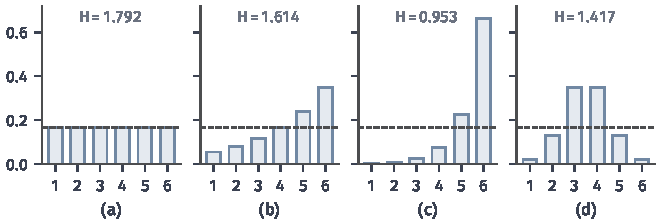
\includegraphics[width=112mm]{figures/07-probability/07-distribution-optimization/matplotlib/dsel-dice-bars/figure.pdf}
 \caption{骰子的最大熵分布（蓝色柱），深灰虚线为均匀概率$1/6$，图中标出熵（nat）。(a)$\mathbb{E}[X]=3.5$，约束不起作用。(b)$\mathbb{E}[X]=4.5$，$\theta\approx0.371$。(c)$\mathbb{E}[X]=5.5$，$\theta\approx1.087$。(d)$\mathbb{E}[X]=3.5$且$\mathbb{E}[(X-3.5)^{2}]=1$，$q\propto\mathrm{e}^{\theta_2(x-3.5)^{2}}$，$\theta_2\approx-0.489$。}
 \label{fig:dsel-dice-bars}
\end{BookInlineFigure}

增加约束只会缩小可行集合，最大熵不会增加；(d)比(a)少了约$0.375$ nat，这就是“方差为$1$”这条信息的量。最大熵还随约束值连续变化。记$H^{*}(m)$为均值为$m$时的最大熵。设$Q_1,Q_2$分别是均值$m_1,m_2$下的最大熵分布，$0\leq\lambda\leq1$，混合$\lambda Q_1+(1-\lambda)Q_2$的均值是$\lambda m_1+(1-\lambda)m_2$，由熵的凹性，
\[
 H^{*}\bigl(\lambda m_1+(1-\lambda)m_2\bigr)\geq H\bigl(\lambda Q_1+(1-\lambda)Q_2\bigr)\geq\lambda H^{*}(m_1)+(1-\lambda)H^{*}(m_2) .
\]
所以$H^{*}$是凹函数。图~\ref{fig:dsel-entropy-curve}(a)中它在$m=3.5$处取最大值$\ln6$，向两端下降，在$m=1$和$m=6$处为零，那里唯一可行的分布是单点分布；(b)中的$\theta(m)$在两端发散，与第~\ref{sec:dsel-moment-matching}节的边界情形一致。

\begin{BookInlineFigure}
 \centering
 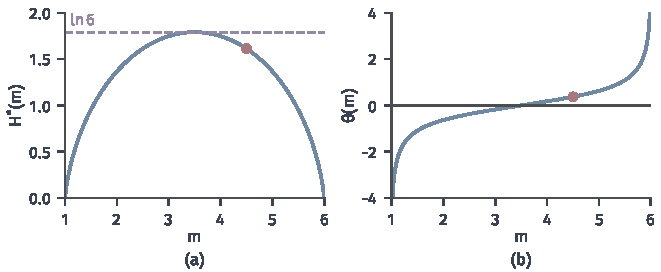
\includegraphics[width=112mm]{figures/07-probability/07-distribution-optimization/matplotlib/dsel-entropy-curve/figure.pdf}
 \caption{骰子均值为$m$时的最大熵问题。(a)最大熵$H^{*}(m)$（蓝），紫色虚线为上界$\ln6$，红点为$m=4.5$，$H^{*}\approx1.614$。(b)对应的乘子$\theta(m)$，红点为$(4.5,\,0.371)$，$m\to1$或$6$时发散。}
 \label{fig:dsel-entropy-curve}
\end{BookInlineFigure}

\paragraph{连续情形的参考测度}
对有密度的分布，第~\ref{chap:information-measures}章用微分熵$h=-\int f\ln f\,\mathrm{d}x$代替熵。这里的密度是相对于Lebesgue测度的密度，Lebesgue测度在其中扮演的角色，正是有限情形中的计数测度。一般地，设$\nu$是$\mathcal{X}$上的$\sigma$有限测度，$Q\ll\nu$，$q=\mathrm{d}Q/\mathrm{d}\nu$，在$q\lvert\ln q\rvert$对$\nu$可积时定义
\begin{equation}
 h_\nu(Q)=-\int_{\mathcal{X}}q\ln q\,\mathrm{d}\nu .
 \label{eq:dsel-entropy-reference}
\end{equation}
换一个参考测度，这个量就变成另一个泛函，最大化它得到的分布也随之不同。

看一个不带任何矩约束的例子：$\mathcal{X}=[1,\mathrm{e}]$。以$\nu=\mathrm{d}x$为参考，$\nu$的总质量是$\mathrm{e}-1$，记$R$为$[1,\mathrm{e}]$上的均匀分布，与式~\eqref{eq:dsel-entropy-kl-uniform}同样计算得
\[
 h_{\mathrm{d}x}(Q)=\ln(\mathrm{e}-1)-D_{\mathrm{KL}}(Q\Vert R),
\]
最大熵分布是均匀分布，密度$1/(\mathrm{e}-1)$。以$\nu(\mathrm{d}x)=\mathrm{d}x/x$为参考，总质量$\int_1^{\mathrm{e}}x^{-1}\,\mathrm{d}x=1$，$\nu$本身就是概率测度，
\[
 h_{\mathrm{d}x/x}(Q)=-D_{\mathrm{KL}}(Q\Vert\nu),
\]
最大熵分布是$\nu$本身，相对$\mathrm{d}x$的密度为$1/x$。换成变量$y=\ln x$，第二个参考测度就是$[0,1]$上的Lebesgue测度，它说的是“$\ln X$均匀”。两个答案的中位数分别是$(1+\mathrm{e})/2\approx1.859$与$\sqrt{\mathrm{e}}\approx1.649$，见图~\ref{fig:dsel-reference-measure}。同样是“一无所知”，用$x$计量还是用$\ln x$计量，给出不同的分布。

\begin{BookInlineFigure}
 \centering
 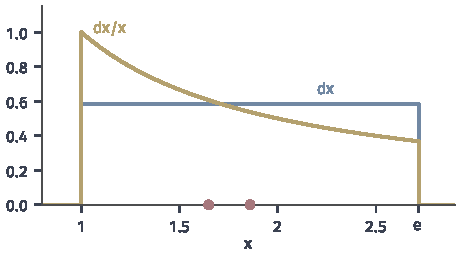
\includegraphics[width=78mm]{figures/07-probability/07-distribution-optimization/matplotlib/dsel-reference-measure/figure.pdf}
 \caption{参考测度决定最大熵分布，$\mathcal{X}=[1,\mathrm{e}]$，无矩约束。蓝：以$\mathrm{d}x$为参考，得到均匀密度$1/(\mathrm{e}-1)$；黄：以$\mathrm{d}x/x$为参考，得到密度$1/x$，即$\ln X$在$[0,1]$上均匀。两个红点是二者的中位数$\sqrt{\mathrm{e}}$与$(1+\mathrm{e})/2$。}
 \label{fig:dsel-reference-measure}
\end{BookInlineFigure}

所以在连续情形中谈最大熵，必须先说明熵是相对哪个测度计算的。有限情形中这个问题被状态集合的选择掩盖了：一旦把骰子的六面当作六个状态，计数测度就是默认的参考。

\paragraph{熵与KL的差别}
在有限情形中，最大熵与以均匀分布为参考的最小KL只差常数。一般的参考概率$P$却不能这样替换。设$P$相对$\nu$的密度$p$处处为正，$Q$相对$\nu$的密度为$q$。在$\{q>0\}$上把$\ln q$拆成$\ln(q/p)+\ln p$，乘以$q$积分，在两项都有限时得到
\begin{equation}
 h_\nu(Q)=-D_{\mathrm{KL}}(Q\Vert P)-\mathbb{E}_{Q}[\ln p] .
 \label{eq:dsel-entropy-kl-reference}
\end{equation}
第二项依赖于$Q$，所以最大化$h_\nu$与最小化$D_{\mathrm{KL}}(\cdot\Vert P)$一般选出不同的分布。负熵$-h_\nu$是“相对于$\nu$”的KL，而不是相对于某个概率分布的KL；在有限情形中两者相同，只因为$\ln p$是常数$-\ln n$。

第二项在可行集合上为常数的情形是例外。若$\ln p$是约束统计量的仿射函数，
\[
 \ln p=\langle\bm{\theta},\bm{T}\rangle-A(\bm{\theta}),
\]
则对每个满足$\mathbb{E}_{Q}[\bm{T}]=\bm{m}$的$Q$，$\mathbb{E}_{Q}[\ln p]$都等于同一个常数$\langle\bm{\theta},\bm{m}\rangle-A(\bm{\theta})$，最大熵与最小KL就重合了。下面的定理正是这样证明的。

\begin{theorem}[相对参考测度的最大熵]
\label{thm:dsel-maxent-continuous}
设$\nu$是$\mathcal{X}$上的$\sigma$有限测度，$\bm{T}:\mathcal{X}\to\mathbb{R}^{k}$可测。设$\bm{\theta}$使
\begin{equation}
 A(\bm{\theta})=\ln\int_{\mathcal{X}}\mathrm{e}^{\langle\bm{\theta},\bm{T}\rangle}\,\mathrm{d}\nu<\infty ,
 \label{eq:dsel-maxent-partition}
\end{equation}
并且相对$\nu$的密度为
\begin{equation}
 q_{\bm{\theta}}=\exp\bigl(\langle\bm{\theta},\bm{T}\rangle-A(\bm{\theta})\bigr)
 \label{eq:dsel-maxent-density}
\end{equation}
的分布$Q_{\bm{\theta}}$满足$\mathbb{E}_{Q_{\bm{\theta}}}\lVert\bm{T}\rVert_2<\infty$，$\mathbb{E}_{Q_{\bm{\theta}}}[\bm{T}]=\bm{m}$。则对每个满足$Q\ll\nu$、$q\lvert\ln q\rvert$对$\nu$可积、$\mathbb{E}_{Q}\lVert\bm{T}\rVert_2<\infty$且$\mathbb{E}_{Q}[\bm{T}]=\bm{m}$的分布$Q$，
\begin{equation}
 h_\nu(Q)=h_\nu(Q_{\bm{\theta}})-D_{\mathrm{KL}}(Q\Vert Q_{\bm{\theta}}),\qquad h_\nu(Q_{\bm{\theta}})=A(\bm{\theta})-\langle\bm{\theta},\bm{m}\rangle .
 \label{eq:dsel-maxent-identity}
\end{equation}
因此$Q_{\bm{\theta}}$是这些分布中熵最大的唯一一个。
\end{theorem}

\begin{proof}
$q_{\bm{\theta}}$处处为正，所以$Q\ll Q_{\bm{\theta}}$，密度比为$q/q_{\bm{\theta}}$。在$\{q>0\}$上，
\[
 \ln\frac{q}{q_{\bm{\theta}}}=\ln q-\langle\bm{\theta},\bm{T}\rangle+A(\bm{\theta}) .
\]
右边三项都在$Q$下可积：$\int q\lvert\ln q\rvert\,\mathrm{d}\nu<\infty$，$\bm{T}$在$Q$下可积，$A(\bm{\theta})$是常数。逐项取$Q$下的期望，
\[
 D_{\mathrm{KL}}(Q\Vert Q_{\bm{\theta}})=-h_\nu(Q)-\langle\bm{\theta},\bm{m}\rangle+A(\bm{\theta}) .
\]
对$Q=Q_{\bm{\theta}}$，由
\[
 \lvert\ln q_{\bm{\theta}}\rvert\leq\lvert\langle\bm{\theta},\bm{T}\rangle\rvert+\lvert A(\bm{\theta})\rvert
\]
知$\ln q_{\bm{\theta}}$在$Q_{\bm{\theta}}$下可积，它满足同样的条件，代入上式，左边为零，得到式~\eqref{eq:dsel-maxent-identity}的第二式。把第二式代回上式，就得到第一式。唯一性来自Gibbs不等式的等号条件。
\end{proof}

定理的形式与有限情形相同，不同之处在于两件事都要事先核对：配分积分$\int\mathrm{e}^{\langle\bm{\theta},\bm{T}\rangle}\mathrm{d}\nu$是否有限，以及候选分布的熵是否有定义。第~\ref{chap:information-measures}章已经指出，密度可以大于$1$，$-q\ln q$有正有负，正负两部分的积分都发散时熵没有意义；这样的分布不在定理比较的范围内。

\paragraph{几个连续例子}
在$\mathbb{R}$上以Lebesgue测度为参考，规定均值$\mu$与方差$\sigma^{2}$，即$\bm{T}(x)=(x,x^{2})$，$\bm{m}=(\mu,\mu^{2}+\sigma^{2})$。候选形式是$\mathrm{e}^{\theta_1x+\theta_2x^{2}}$，可积要求$\theta_2<0$，它就是高斯密度；$\mathcal{N}(\mu,\sigma^{2})$满足约束，由定理~\ref{thm:dsel-maxent-continuous}，它是给定均值与方差的密度中微分熵最大的，最大值为
\[
 h\bigl(\mathcal{N}(\mu,\sigma^{2})\bigr)=\frac12\ln(2\pi\mathrm{e}\sigma^{2}) .
\]
方差为$1$时它约为$1.419$。同样方差为$1$的Laplace密度微分熵约为$1.347$，$[-\sqrt3,\sqrt3]$上的均匀密度约为$1.242$，都更小，见图~\ref{fig:dsel-gauss-maxent}。

\begin{BookInlineFigure}
 \centering
 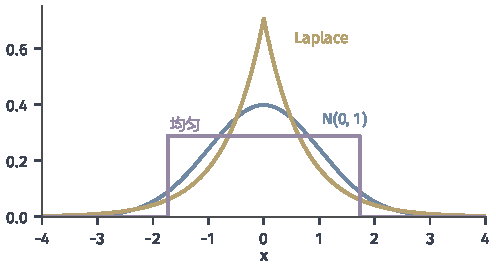
\includegraphics[width=84mm]{figures/07-probability/07-distribution-optimization/matplotlib/dsel-gauss-maxent/figure.pdf}
 \caption{均值$0$、方差$1$的三个密度。蓝：$\mathcal{N}(0,1)$，$h=\frac12\ln(2\pi\mathrm{e})\approx1.419$；黄：尺度$1/\sqrt2$的Laplace密度，$h=1+\ln\sqrt2\approx1.347$；紫：$[-\sqrt3,\sqrt3]$上的均匀密度，$h=\ln(2\sqrt3)\approx1.242$。熵相对Lebesgue测度计算，单位为nat。}
 \label{fig:dsel-gauss-maxent}
\end{BookInlineFigure}

在$(0,\infty)$上规定均值$1/\lambda$，候选$\mathrm{e}^{\theta x}$要求$\theta<0$，得到$\operatorname{Exp}(\lambda)$，最大熵为$1-\ln\lambda$。在有界区间$[a,b]$上不加任何矩约束，$\bm{T}=\bm{0}$，得到均匀分布，最大熵为$\ln(b-a)$。这三个常见分布都是“在某个支持上、给定某些矩”时的最大熵分布，支持与矩缺一不可。

最大值也可能不存在。在$\mathbb{R}$上只规定均值$\mu$，候选形式$\mathrm{e}^{\theta x}$对任何$\theta$都不可积，定理无从适用；而$\mathcal{N}(\mu,s^{2})$都满足约束，熵$\frac12\ln(2\pi\mathrm{e}s^{2})$随$s\to\infty$趋于无穷，所以上确界是$+\infty$。在$(0,\infty)$上不加约束也是如此。Lebesgue测度的总质量无穷，质量可以无限摊开，熵就没有上界。


\section{解的检验}
\label{sec:dsel-checks}

前三节都先用乘子或驻点“猜”出解的形式，再用一个恒等式验证它。实际计算中，候选分布还可能来自截断的级数、数值迭代或随机估计，它未必满足原问题的全部要求。拿到一个候选$\widehat{Q}$后，应当回到原问题依次回答三个问题：它是不是合法的候选，最小值存不存在，它是否达到了最小值或离最小值还有多远。图~\ref{fig:dsel-check-flow}把这些检查排成一条链。

\begin{BookInlineFigure}
 \centering
 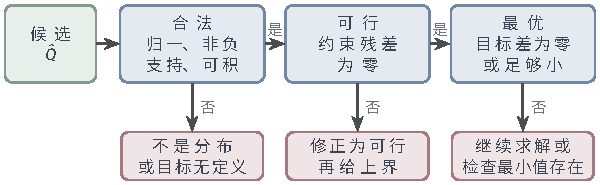
\includegraphics[width=102mm]{figures/07-probability/07-distribution-optimization/tikz/dsel-check-flow/figure.pdf}
 \caption{候选分布的检查顺序。绿框是待检的候选，蓝框是依次要通过的检查，红框是未通过时的处理：不合法的候选不能参加比较；不满足约束的候选先修正为可行分布，再用于给出最优值的上界；目标差不够小时继续求解，或回头检查最小值是否存在。}
 \label{fig:dsel-check-flow}
\end{BookInlineFigure}

\paragraph{候选是否合法}
第一步核对第~\ref{sec:dsel-problems}节列出的各项。归一化与非负性：指数形式的公式保证非负，但若配分函数是截断级数或数值积分得到的，归一化可能只是近似成立。支持：所有候选都要满足$\widehat{Q}\ll P$；倾斜公式自动满足，边界解则需要明确哪些状态的概率为零。可积性：目标与约束中的期望都要有限，下面会看到一个写得出公式、却因可积性失败而不合法的例子。

约束问题还要检查约束残差$\bm{r}=\mathbb{E}_{\widehat{Q}}[\bm{T}]-\bm{m}$。以第~\ref{sec:dsel-moment-matching}节Newton法的第一步为例，$\theta^{(1)}=9/14$给出
\[
 \widehat{Q}=Q_{\theta^{(1)}}\approx(0.1534,\ 0.2917,\ 0.5549),\qquad r\approx1.40147-1.42857=-0.0271 .
\]
它不满足约束，不属于可行集合。这时它的KL值$D_{\mathrm{KL}}(\widehat{Q}\Vert P)\approx0.1248$比真正的最优值$0.1429$还小，若把它当作“最小KL”报告就错了：违反约束的候选可以比最优解更好。

\paragraph{目标差}
不可行的倾斜分布并非没有用处。式~\eqref{eq:dsel-weak-duality}说明，任何$\bm{\theta}$都给出最优值的下界$\ell(\bm{\theta})$；再把$\widehat{Q}$修正成一个可行分布$\widetilde{Q}$，就得到上界$D_{\mathrm{KL}}(\widetilde{Q}\Vert P)$。两者之差
\begin{equation}
 D_{\mathrm{KL}}(\widetilde{Q}\Vert P)-\ell(\bm{\theta})\geq D_{\mathrm{KL}}(\widetilde{Q}\Vert P)-D^{*}\geq0
 \label{eq:dsel-certificate}
\end{equation}
控制了$\widetilde{Q}$离最优还差多少，这就是\term{最优性证书}（optimality certificate）：不必知道$D^{*}$，就能保证误差不超过一个算得出的数。

在例子中，$\widehat{Q}$的均值偏小，把它与均值最大的点质量$\delta_2$混合：
\[
 \widetilde{Q}=(1-\alpha)\widehat{Q}+\alpha\delta_2 ,
\]
均值为$(1-\alpha)\cdot1.40147+2\alpha$。令它等于$10/7$，解得
\[
 \alpha=\frac{10/7-1.40147}{2-1.40147}\approx0.04528 .
\]
修正后的$\widetilde{Q}\approx(0.1464,0.2785,0.5750)$可行，上界与下界分别为
\[
 D_{\mathrm{KL}}(\widetilde{Q}\Vert P)\approx0.143059,\qquad\ell(\theta^{(1)})=\frac{10}{7}\cdot\frac{9}{14}-A\Bigl(\frac9{14}\Bigr)\approx0.142234 .
\]
两者相差约$8.3\times10^{-4}$，所以$\widetilde{Q}$的KL离最优值不超过$8.3\times10^{-4}$，而最优值被夹在$[0.142234,\ 0.143059]$中。

对后续的Newton迭代点做同样的事，得到表~\ref{tab:dsel-certificate}与图~\ref{fig:dsel-certificate}。第二步之后证书已小于$2\times10^{-7}$，第三步约为$10^{-14}$，与数值舍入相当。

\begin{BookInlineTable}
 \centering
 \caption{Newton迭代点的最优性证书，$P$均匀，$T(x)=x$，$m=10/7$，精确最优值$D^{*}\approx0.1429124$。$\alpha$是为满足约束而混入$\delta_2$的比例。}
 \label{tab:dsel-certificate}
 \begin{tabular}{ccccc}
 \toprule
 $t$ & $\theta^{(t)}$ & 下界$\ell(\theta^{(t)})$ & 上界$D_{\mathrm{KL}}(\widetilde{Q}\Vert P)$ & 证书 \\
 \midrule
 $0$ & $0$ & $0$ & $0.170028$ & $1.7\times10^{-1}$ \\
 $1$ & $0.642857$ & $0.142234$ & $0.143059$ & $8.3\times10^{-4}$ \\
 $2$ & $0.692394$ & $0.1429122$ & $0.1429124$ & $1.8\times10^{-7}$ \\
 $3$ & $0.693147$ & $0.1429124$ & $0.1429124$ & $1.0\times10^{-14}$ \\
 \bottomrule
 \end{tabular}
\end{BookInlineTable}

\begin{BookInlineFigure}
 \centering
 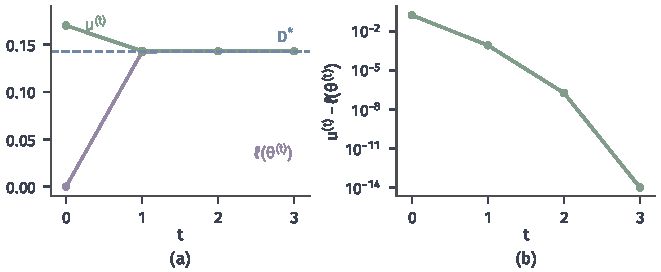
\includegraphics[width=112mm]{figures/07-probability/07-distribution-optimization/matplotlib/dsel-certificate/figure.pdf}
 \caption{最优性证书随Newton迭代的变化。(a)下界$\ell(\theta^{(t)})$（紫）与修正后可行分布的上界$u^{(t)}=D_{\mathrm{KL}}(\widetilde{Q}\Vert P)$（绿），蓝色虚线是$D^{*}$。(b)证书$u^{(t)}-\ell(\theta^{(t)})$，纵轴为对数刻度。}
 \label{fig:dsel-certificate}
\end{BookInlineFigure}

证书的两部分各有含义。在式~\eqref{eq:dsel-pythagoras-general}中分别取$Q=\widetilde{Q}$与$Q=Q^{*}$，得到
\[
 D_{\mathrm{KL}}(\widetilde{Q}\Vert P)-D^{*}=D_{\mathrm{KL}}(\widetilde{Q}\Vert Q^{*}),\qquad D^{*}-\ell(\bm{\theta})=D_{\mathrm{KL}}(Q^{*}\Vert Q_{\bm{\theta}}) .
\]
上界的误差是可行候选离最优分布的KL，下界的误差是最优分布离当前倾斜分布的KL。在第一步，两者约为$1.5\times10^{-4}$与$6.8\times10^{-4}$，和正是表中的$8.3\times10^{-4}$。

KL正则化的成本问题更直接。若$Z$能算出，最优值就是$-\tau\ln Z$，由式~\eqref{eq:dsel-gibbs-identity}，任何候选的目标差恰为$\tau D_{\mathrm{KL}}(\widehat{Q}\Vert Q^{*})$，不需要另找下界。

\paragraph{最小值是否存在}
有限状态上，可行集合非空时它是概率单纯形中的有界闭集，目标若在其上连续，最小值必然取到；第~\ref{sec:dsel-moment-matching}节的边界定理就是这样证明的。状态无穷时，这个论证会失效。

取$\mathcal{X}=\{1,2,\dots\}$，$P(k)=c/k^{3}$，$c=1/\sum_kk^{-3}\approx0.8319$。$P$的均值有限，
\[
 \mu=\mathbb{E}_{P}[X]=c\sum_{k\geq1}\frac1{k^{2}}=\frac{c\,\pi^{2}}{6}\approx1.3684 .
\]
要求$\mathbb{E}_{Q}[X]=2$，在可行分布中最小化$D_{\mathrm{KL}}(Q\Vert P)$。

先试倾斜。$q_\theta(k)\propto\mathrm{e}^{\theta k}/k^{3}$，当$\theta>0$时级数发散，倾斜分布不存在；当$\theta\leq0$时倾斜分布存在，但均值关于$\theta$不减（导数是方差），所以均值不超过$\theta=0$时的$\mu<2$。没有任何倾斜分布满足约束。

再看最优值。令$Q_N=(1-\varepsilon)P+\varepsilon\delta_N$，其中$\varepsilon=(2-\mu)/(N-\mu)$，它的均值是$\mu+\varepsilon(N-\mu)=2$，可行。$Q_N$与$P$的密度比在$k\neq N$处是$1-\varepsilon$，在$k=N$处是$1-\varepsilon+\varepsilon/P(N)$，所以
\[
 D_{\mathrm{KL}}(Q_N\Vert P)=(1-\varepsilon)\bigl(1-P(N)\bigr)\ln(1-\varepsilon)+Q_N(N)\ln\Bigl(1-\varepsilon+\frac{\varepsilon N^{3}}{c}\Bigr).
\]
第一项趋于零。第二项中$Q_N(N)\leq P(N)+\varepsilon$约为$0.632/N$，对数约为$2\ln N$，乘积约为$1.26\ln N/N$，也趋于零。数值上，$N=10,100,1000,10^{4}$时KL分别约为$0.261$、$0.0509$、$0.00793$、$0.00108$。所以最优值是$0$。

但最优值$0$达不到：$D_{\mathrm{KL}}(Q\Vert P)=0$只对$Q=P$成立，而$P$的均值是$1.3684$，不是$2$。图~\ref{fig:dsel-heavy-tail}画出这个机制：把极小的质量放到很远的地方，均值就能提高很多，KL的代价却微不足道。$Q_N$与$P$的总变差是$\varepsilon(1-P(N))\to0$，可是均值始终是$2$；函数$x$无界，均值不随分布的这种接近而连续变化，可行集合在这种收敛下不是闭的。

\begin{BookInlineFigure}
 \centering
 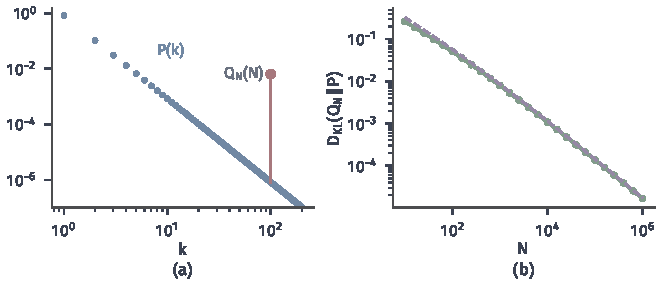
\includegraphics[width=112mm]{figures/07-probability/07-distribution-optimization/matplotlib/dsel-heavy-tail/figure.pdf}
 \caption{最小KL达不到的例子。$P(k)=c/k^{3}$，约束$\mathbb{E}_{Q}[X]=2$。(a)$P$的质量（蓝点），双对数坐标；$Q_{100}$把每项乘以$1-\varepsilon$，并在$k=100$处加上质量$\varepsilon\approx0.0064$（红）。(b)$D_{\mathrm{KL}}(Q_N\Vert P)$（绿）随$N$趋于零，紫色虚线是近似$\varepsilon\ln(\varepsilon N^{3}/c)$。}
 \label{fig:dsel-heavy-tail}
\end{BookInlineFigure}

一般空间中的存在性需要两方面的条件。一方面，KL的下水平集$\{Q:D_{\mathrm{KL}}(Q\Vert P)\leq a\}$在分布的弱收敛下是紧的，并且$D_{\mathrm{KL}}(\cdot\Vert P)$下半连续；证明需要用到下半连续函数的变分表示和第~\ref{chap:weak-convergence-of-distributions}章的胎紧性，可查阅~\scite{math-kallenberg2021probability}。另一方面，约束集合要在弱收敛下闭，例如$\bm{T}$有界连续时就是如此。两者都成立、且可行集合中有KL有限的分布时，最小值能取到。上面的例子缺的是第二条。

\paragraph{给出的分布是否达到最小值}
即使最优值有限、公式也写得出来，写出的分布仍可能不是候选。回到KL正则化的成本问题，取$\mathcal{X}=\{1,2,\dots\}$，$\tau=1$，
\[
 P(k)=c'\,\frac{\mathrm{e}^{-k}}{k^{2}},\qquad V(k)=-k ,
\]
其中$c'=1/\sum_k\mathrm{e}^{-k}k^{-2}\approx2.4465$。配分函数是
\[
 Z=\sum_{k\geq1}c'\frac{\mathrm{e}^{-k}}{k^{2}}\mathrm{e}^{k}=c'\frac{\pi^{2}}{6}\approx4.024 ,
\]
有限，Gibbs分布$Q^{*}(k)=\frac{6}{\pi^{2}k^{2}}$存在。可是
\[
 \mathbb{E}_{Q^{*}}\lvert V\rvert=\frac{6}{\pi^{2}}\sum_{k\geq1}\frac1k=\infty ,
\]
$Q^{*}$不在候选集合$\mathcal{Q}_V$中，定理~\ref{thm:dsel-gibbs-variational}的第二部分不适用。

第一部分仍然成立：对每个$Q\in\mathcal{Q}_V$，
\[
 J_1(Q)=-\ln Z+D_{\mathrm{KL}}(Q\Vert Q^{*})>-\ln Z ,
\]
严格不等号是因为$Q\neq Q^{*}$。另一方面，截断$Q_N=Q^{*}(\cdot\mid k\leq N)$只有有限个状态，属于$\mathcal{Q}_V$，并且
\[
 D_{\mathrm{KL}}(Q_N\Vert Q^{*})=-\ln Q^{*}(\{k\leq N\})\to0 .
\]
$N=10,100,1000$时它约为$0.060$、$0.0061$、$0.00061$。所以最优值是$-\ln Z\approx-1.392$，但没有候选达到它。只检查“公式里的$Z$有限”是不够的，还要检查公式给出的分布本身满足候选集合的可积性要求。

\paragraph{期望无法直接计算时}
上面的检查都需要计算期望：配分函数、矩、协方差、KL。状态数很大或空间连续时，这些量本身是难算的积分，常用随机抽样的平均来估计，估计值带有随机误差。这时约束残差与证书也只是估计：一个看起来很小的证书，可能只是估计误差掩盖了真实的差距。用抽样估计这些期望时，应当按第~\ref{chap:monte-carlo-integration-error}章的方法给出误差范围，并把它计入残差与证书，而不是只报告点估计。


\section{本章小结}
\label{sec:dsel-summary}

本章把概率分布当作未知量，在允许的分布中按目标与约束选出一个。章首三种愿望的分歧有了明确的回答：降低期望成本是要最小化的线性目标，单独使用会把质量推到顶点；指定平均量是等式约束，单独使用留下无穷多个候选；接近参考分布是以KL计量的代价，单独使用什么也不改变。把它们组合成一个问题，再写清候选集合中的非负性、归一化、支持与可积性，问题才有确定的含义；第一节的可数例子说明，省略可积性会让目标变成依赖配对方式的“$-\infty+\infty$”。

三类问题的解都是“参考测度乘以指数权重再归一化”，但各自的来源与条件不同，表~\ref{tab:dsel-summary}把它们并列。

\begin{BookInlineTable}
 \centering
 \caption{本章三类分布选择问题。$A(\bm{\theta})$是以参考测度为基准的对数配分函数，$Z=\mathbb{E}_{P}[\mathrm{e}^{-V/\tau}]$。矩约束最小KL的条件指有限状态、参考概率处处为正的情形；最大熵还要求候选分布的熵有定义。}
 \label{tab:dsel-summary}
 \small
 \begin{tabular}{llll}
 \toprule
 问题 & 解的形式 & 最优值 & 主要条件 \\
 \midrule
 KL正则化成本 & $\mathrm{d}Q^{*}/\mathrm{d}P\propto\mathrm{e}^{-V/\tau}$ & $-\tau\ln Z$ & $Z<\infty$，$V\in L^{1}(Q^{*})$ \\
 矩约束最小KL & $\mathrm{d}Q^{*}/\mathrm{d}P\propto\mathrm{e}^{\langle\bm{\theta},\bm{T}\rangle}$ & $\langle\bm{\theta},\bm{m}\rangle-A(\bm{\theta})$ & $\bm{m}\in\operatorname{ri}\mathcal{M}$ \\
 最大熵 & $\mathrm{d}Q^{*}/\mathrm{d}\nu\propto\mathrm{e}^{\langle\bm{\theta},\bm{T}\rangle}$ & $A(\bm{\theta})-\langle\bm{\theta},\bm{m}\rangle$ & 配分积分有限 \\
 \bottomrule
 \end{tabular}
\end{BookInlineTable}

Gibbs分布由KL正则化的成本问题给出，它的最优性由恒等式~\eqref{eq:dsel-gibbs-identity}证明：任何候选比最优值多出的部分恰是$\tau D_{\mathrm{KL}}(Q\Vert Q^{*})$。指数倾斜由矩约束下的最小KL给出，最优性由勾股恒等式证明，求解归结为$k$个未知数的矩匹配方程；方程的Jacobian是统计量的协方差，冗余统计量使参数不唯一而分布仍唯一，边界上的矩使最优分布收缩支持、参数发散。最大熵在有限支持上就是以均匀分布为参考的最小KL；在连续情形中熵依赖于参考测度，只有参考密度的对数是约束统计量的仿射函数时，最大熵才与最小KL重合。

这三种解的指数形式都是由最优性推出来的，不是预先选定的分布族。公式只给出候选，第五节的检查把“候选合法”“最小值存在”“候选达到最小值”分开处理：对偶下界与可行上界之差给出可计算的最优性证书；无穷状态上最小值可能达不到，写得出的Gibbs分布也可能因可积性失败而不是候选。

本章的出发点是参考分布与约束，目标分布并不存在，要选的就是它。下一章换一个起点：目标分布已经给定，但难以计算，我们限制候选集合，在容易表示和使用的分布中寻找它的近似。那时KL的两个方向、候选族的表达能力与逼近误差，成为需要分别研究的问题。


\chapter{概率分布的逼近}
\label{chap:distribution-approximation}

实数轴上有一个分布，我们只知道它的密度正比于
\[
 \widetilde{\pi}(x)=\mathrm{e}^{-x^{4}/4} .
\]
任给一个$x$，$\widetilde{\pi}(x)$都能立即算出；可是要回答“$X$落在$[-1,1]$外的概率是多少”“$X^{2}$的平均是多少”，就要先求归一化常数$\int\widetilde{\pi}\,\mathrm{d}x$，再做积分。一维时数值积分不难，若变量有几十个分量，同样的积分就无法逐格计算。一个自然的想法是找一个容易计算的分布，比如某个高斯分布，代替它回答这些问题。

这样做立刻带来四个问题。第一，候选分布从哪里选：所有高斯分布，所有各分量独立的分布，还是某个有限维参数族？候选集合定下以后，有些性质无论怎样选都保留不下来。第二，“最接近”按什么标准：第~\ref{chap:distribution-comparison}章的KL散度有两个方向，分别按候选分布和按目标分布加权，选出的分布一般不同。第三，怎样求出最接近的候选：有时能逐个因子写出最优更新，有时只能对参数做梯度下降。第四，得到的近似有多好：误差既来自候选集合的表达能力，也来自没有算到最优，还来自期望的数值计算。

本章依次回答这四个问题。第一节固定目标分布，区分候选分布能计算密度、能抽样和能求期望这几项不同的要求，并用两个变量的概率表说明结构限制怎样删去依赖。第二节分别研究两个方向的KL目标，说明各自的支持条件、权重与计算需求，并在一个三点分布的例子中算出两个方向的最优解。第三节把候选限制为乘积分布，先在相关高斯分布上看独立性限制改变了哪些数值特征，再推导逐因子的坐标更新。第四节处理有限维参数族上的梯度更新。第五节把误差分成几个来源，说明怎样按任务检验近似结果。

本章回用第~\ref{chap:distribution-families}章的分布族，特别是指数族的对数配分函数与均值参数；第~\ref{chap:distribution-comparison}章的KL散度、Gibbs不等式与Pinsker不等式；第~\ref{chap:information-measures}章的交叉熵与互信息。上一章在满足约束的全体分布中选择分布，那里的最优解由问题本身给出；本章的目标分布已经给定，困难在于候选集合受到限制。

\section{目标分布与候选族}
\label{sec:dapx-target-candidates}

逼近问题有两个输入：要逼近的分布，以及允许用来逼近的分布。前者在本章中始终固定，后者由我们选择。选择候选集合时，首先要弄清“容易计算”具体指哪几种计算，其次要弄清限制候选集合会丢掉什么，最后要检查逼近目标对这两个集合是否有定义。

\paragraph{目标分布}
设取值空间$\mathcal{X}$上有一个概率分布$\Pi$，称为\term{目标分布}（target distribution）。取一个参考测度$\lambda$：有限或可数的$\mathcal{X}$上取计数测度，$\mathbb{R}^{d}$上取Lebesgue测度。设$\Pi\ll\lambda$，密度记为$\pi$。很多时候我们只知道
\begin{equation}
 \pi(x)=\frac{\widetilde{\pi}(x)}{Z},\qquad Z=\int_{\mathcal{X}}\widetilde{\pi}\,\mathrm{d}\lambda,\qquad 0<Z<\infty ,
 \label{eq:dapx-unnormalized}
\end{equation}
其中$\widetilde{\pi}\geq0$可以逐点计算，称为\term{未归一化密度}（unnormalized density），而$Z$算不出来。条件$0<Z<\infty$保证$\Pi$是一个合法的概率分布；它是逼近问题的前提，不是逼近要解决的问题。

计算困难通常来自维数。设$\bm{x}=(x_1,\dots,x_m)\in\{0,1\}^{m}$，未归一化密度由成对的相互作用给出，
\[
 \widetilde{\pi}(\bm{x})=\exp\Bigl(\sum_{i<j}J_{i,j}x_ix_j+\sum_{i}h_ix_i\Bigr) .
\]
任给一个$\bm{x}$，计算$\widetilde{\pi}(\bm{x})$只需要做$m(m-1)/2+m$次乘加。$Z$却是$2^{m}$项之和，$m=50$时约$10^{15}$项；边缘概率$\Pi(X_1=1)$也要对其余$49$个分量的$2^{49}$种取值求和。密度可以逐点算，却不等于概率和期望可以算。

\paragraph{候选集合与三种计算}
用来逼近的分布组成\term{候选集合}（candidate set）$\mathcal{Q}$，其中每个$Q$也对$\lambda$有密度$q$。第~\ref{chap:distribution-families}章给出了构造候选集合的几种方式：有限维参数族$\{q_{\bm{\theta}}:\bm{\theta}\in\Theta\}$、指数族、混合分布、由简单随机变量经变换得到的推前族。选哪一种，要看后面需要对候选分布做哪些计算。这些计算可以分成三项：
\begin{itemize}
 \item \textbf{计算密度}：任给$x$，算出$q(x)$或$\ln q(x)$，有时允许差一个常数；
 \item \textbf{抽样}：生成服从$Q$的独立样本；
 \item \textbf{求期望}：对给定的函数$f$，算出$\mathbb{E}_{Q}[f(X)]$的准确值或足够准确的近似。
\end{itemize}
三项能力相互独立，有一项不代表有另一项。表~\ref{tab:dapx-abilities}列出几类常见分布的情况。

\begin{BookInlineTable}
 \centering
 \caption{几类分布在三项计算上的情况。“是”指有闭式或可以直接执行的算法；求期望一栏针对后文常用的$\mathbb{E}[\ln q(X)]$与低次多项式的期望。}
 \label{tab:dapx-abilities}
 \begin{tabular}{llll}
  \toprule
  分布 & 密度 & 抽样 & 期望\\
  \midrule
  高斯分布 & 是 & 是 & 是\\
  有限状态乘积 & 是 & 是 & 逐因子求和\\
  高斯混合 & 是 & 是 & $\ln q$的期望无闭式\\
  推前族$X=g(Z)$ & 需可逆换元 & 是 & 借助样本\\
  未归一化目标 & 差常数$Z$ & 一般不能 & 一般不能\\
  \bottomrule
 \end{tabular}
\end{BookInlineTable}

高斯混合的密度是几个高斯密度的加权和，可以逐点计算，抽样也只需先抽成分再抽高斯；但$\ln q$是和的对数，它在$Q$下的期望没有闭式，只能数值计算。推前族由$X=g(Z)$定义，$Z$容易抽样，于是$X$也容易抽样；可是$X$的密度要用换元公式，需要$g$可逆、可微并能算Jacobian行列式，否则密度可能根本不存在（第~\ref{chap:distribution-families}章中，$g$把低维的随机变量送进高维空间时，输出落在一个零测集上，就没有密度）。所以，“有一个解析的密度表达式”或“能抽样”都不能代表后续所有计算都已可行，必须对照逼近目标实际需要的计算逐项核对。

\paragraph{结构限制删去依赖}
候选集合的限制不只是“分布形状更简单”，还可能直接删去目标中的某种关系。取两个二值变量，目标分布由概率表给出：
\begin{equation}
 \pi(0,0)=\pi(1,1)=0.45,\qquad \pi(0,1)=\pi(1,0)=0.05 .
 \label{eq:dapx-table}
\end{equation}
两个变量各自取$0$和$1$的概率都是$\tfrac12$，但它们几乎总是相等：$\Pi(X_1=X_2)=0.9$。现在只允许用乘积分布$q(x_1,x_2)=q_1(x_1)q_2(x_2)$逼近它，即$X_1,X_2$在候选分布下独立。记$a=q_1(1)$，$b=q_2(1)$，则
\[
 Q(X_1=X_2)=(1-a)(1-b)+ab .
\]

若要求候选保留目标的两个边缘，必须$a=b=\tfrac12$，此时$Q(X_1=X_2)=\tfrac12$，远小于$0.9$。若要让$Q(X_1=X_2)$接近$0.9$，就要把$a,b$同时推向$0$或同时推向$1$，边缘又不再是$\tfrac12$。乘积候选不能同时保留两个边缘和“两个变量常常相等”这一事实，无论怎样选择$a,b$都是如此。图~\ref{fig:dapx-table-product}画出目标表和它的边缘乘积：对角线上的集中完全消失了。

\begin{BookInlineFigure}
 \centering
 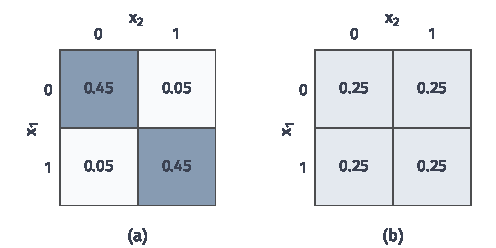
\includegraphics[width=84mm]{figures/07-probability/07-distribution-optimization/matplotlib/dapx-table-product/figure.pdf}
 \caption{结构限制删去依赖。(a)式~\eqref{eq:dapx-table}的目标概率表，行是$x_1$，列是$x_2$，颜色越深概率越大。(b)它的两个边缘都是$(\tfrac12,\tfrac12)$，边缘乘积在四格上都是$0.25$。}
 \label{fig:dapx-table-product}
\end{BookInlineFigure}

这里丢掉的东西可以用第~\ref{chap:information-measures}章的互信息度量。目标与它的边缘乘积之间的KL散度就是$I(X_1;X_2)$，计算得
\[
 D_{\mathrm{KL}}(\Pi\Vert\Pi_1\otimes\Pi_2)=0.9\ln\frac{0.45}{0.25}+0.1\ln\frac{0.05}{0.25}=0.9\ln1.8-0.1\ln5\approx0.3681 .
\]
第~\ref{sec:dapx-mean-field}节将证明，在按目标加权的方向上，这个数恰好是乘积候选所能达到的最小KL；在另一个方向上，最优的乘积分布并不是边缘乘积。

\paragraph{支持、参数范围与可积性}
选定候选集合后，还要检查逼近目标在这两个集合之间是否有意义。第一项检查是支持。设目标是$\operatorname{Exp}(1)$，密度在$x<0$处为零，候选集合是全体一维高斯分布。每个高斯分布都给$(-\infty,0)$正概率，所以$Q\ll\Pi$不成立；按第~\ref{chap:distribution-comparison}章的约定，$D_{\mathrm{KL}}(Q\Vert\Pi)=+\infty$对每个候选成立，这个方向的KL无法区分任何两个候选。另一个方向$D_{\mathrm{KL}}(\Pi\Vert Q)$则对每个高斯候选有限，因为高斯密度处处为正。图~\ref{fig:dapx-support}(a)中红色区域就是候选有质量而目标没有的部分。

第二项检查是参数范围。参数必须落在使候选成为合法分布的集合内：标准差为正，概率表的分量非负且和为$1$，协方差矩阵对称正定，混合权重在单纯形上。优化时这些都是约束，第~\ref{sec:dapx-gradient}节会用重新参数化来自动满足它们。

第三项检查是可积性。绝对连续只保证对数比几乎处处有限，不保证它的期望有限。取目标为标准Cauchy分布，候选为$\mathcal{N}(0,1)$。两个密度处处为正，但
\[
 \ln\frac{\pi(x)}{q(x)}=\frac{x^{2}}{2}-\ln(1+x^{2})+\ln\sqrt{\frac{2}{\pi}} ,
\]
它在Cauchy分布下的期望含有$\mathbb{E}_{\Pi}[X^{2}]=+\infty$，所以$D_{\mathrm{KL}}(\Pi\Vert Q)=+\infty$。把$\mathcal{N}(0,1)$换成任何其他高斯分布，对数比中仍有$x^{2}$的正系数项，结论不变：这个方向对全体高斯候选都是无穷大。反方向的被积函数在高斯权重下迅速衰减，$D_{\mathrm{KL}}(Q\Vert\Pi)$有限，数值积分给出约$0.259$。

\begin{BookInlineFigure}
 \centering
 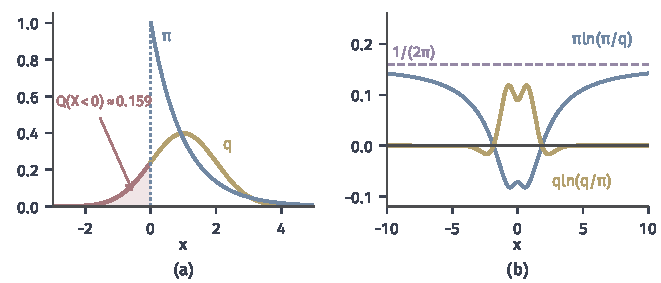
\includegraphics[width=112mm]{figures/07-probability/07-distribution-optimization/matplotlib/dapx-support/figure.pdf}
 \caption{逼近目标可能对所有候选都无穷大。(a)目标$\operatorname{Exp}(1)$（蓝）与候选$\mathcal{N}(1,1)$（黄），红色区域是候选落在$x<0$的质量$\Phi(-1)\approx0.159$，目标在那里没有质量，所以$D_{\mathrm{KL}}(Q\Vert\Pi)=+\infty$。(b)目标为标准Cauchy分布、候选为$\mathcal{N}(0,1)$时两个方向的被积函数：蓝线$\pi\ln(\pi/q)$在远处趋于常数$1/(2\pi)$（紫色虚线），积分发散；黄线$q\ln(q/\pi)$迅速衰减。}
 \label{fig:dapx-support}
\end{BookInlineFigure}

图~\ref{fig:dapx-support}(b)显示了无穷大的来源：Cauchy分布在远处的密度约为$1/(\pi x^{2})$，乘上对数比中的$x^{2}/2$后趋于常数$1/(2\pi)$，在整条直线上积分必然发散。这两个例子说明，KL目标是否有限取决于目标、候选与方向三者的组合。确定候选集合时就要检查它，不能留到优化出问题时再发现。

\section{逼近目标}
\label{sec:dapx-objectives}

候选集合定下以后，要从中挑一个“离目标最近”的分布。第~\ref{chap:distribution-comparison}章给了许多比较分布的量，本章以KL散度为主，因为它的对数比可以按候选分布或目标分布逐点平均，后面的坐标更新和梯度更新都由此推出。KL散度不对称，于是有两个逼近问题：
\begin{equation}
 \min_{Q\in\mathcal{Q}}D_{\mathrm{KL}}(Q\Vert\Pi),\qquad \min_{Q\in\mathcal{Q}}D_{\mathrm{KL}}(\Pi\Vert Q) .
 \label{eq:dapx-two-problems}
\end{equation}
前者的期望按候选分布$Q$计算，后者按目标分布$\Pi$计算。用来做平均的分布不同，带来三处差别：误差在哪里被计入，KL有限需要什么支持条件，计算时需要能对哪个分布求期望。

先说明本节结论的范围。KL散度只是一种比较量。若后续任务关心的是某个事件的概率、某个矩或某个距离，应当按第~\ref{chap:distribution-comparison}章的方法对相应的量另行检查，第~\ref{sec:dapx-error}节会做这样的检查。使某个KL最小的候选，并不自动使其他比较量也最小。

\subsection{按候选分布计算KL}
\label{sec:dapx-reverse-kl}

第一个问题是
\begin{equation}
 \min_{Q\in\mathcal{Q}}D_{\mathrm{KL}}(Q\Vert\Pi)=\min_{Q\in\mathcal{Q}}\mathbb{E}_{Q}\Bigl[\ln\frac{q(X)}{\pi(X)}\Bigr] .
 \label{eq:dapx-reverse-problem}
\end{equation}
它在文献中常称为\term{反向KL散度}（reverse KL divergence）的最小化，“反向”是相对于下一小节按目标加权的方向而言。

\paragraph{误差按候选分布计入}
被积函数$q\ln(q/\pi)$只在候选有质量的地方才有分量。候选给某处很高的概率而目标在那里概率很小，对数比$\ln(q/\pi)$很大，又乘以较大的权重$q$，代价很重。反过来，目标在某处有质量而候选在那里几乎没有质量，权重$q$接近零，这一处几乎不计入。所以这个方向主要惩罚“候选在目标稀少的地方放了质量”，而对“候选漏掉了目标的一部分”宽容得多。

\paragraph{有限的条件}
由第~\ref{chap:distribution-comparison}章的定义，$D_{\mathrm{KL}}(Q\Vert\Pi)<\infty$首先要求$Q\ll\Pi$：候选不能把正概率放在目标概率为零的集合上。上一节的$\operatorname{Exp}(1)$目标与高斯候选就违反这一条。其次，对数比的负部总是可积的，所以在$Q\ll\Pi$时，KL有限当且仅当$\ln(q/\pi)$的正部在$Q$下可积。

\paragraph{未归一化目标}
目标只以式~\eqref{eq:dapx-unnormalized}的形式给出时，把$\pi=\widetilde{\pi}/Z$代入对数比：
\[
 \ln\frac{q(x)}{\pi(x)}=\ln q(x)-\ln\widetilde{\pi}(x)+\ln Z .
\]
$\ln Z$是与$x$和$Q$都无关的常数。设$\ln q-\ln\widetilde{\pi}$在$Q$下可积，记
\begin{equation}
 J(Q)=\mathbb{E}_{Q}\bigl[\ln q(X)-\ln\widetilde{\pi}(X)\bigr] .
 \label{eq:dapx-J}
\end{equation}
对上式取$Q$下的期望，就得到
\begin{equation}
 D_{\mathrm{KL}}(Q\Vert\Pi)=J(Q)+\ln Z .
 \label{eq:dapx-J-shift}
\end{equation}

式~\eqref{eq:dapx-J-shift}有三个推论。第一，在候选集合上最小化$J$与最小化$D_{\mathrm{KL}}(Q\Vert\Pi)$得到同一个最优解，而计算$J$只需要逐点算$\widetilde{\pi}$并对$Q$求期望，不需要$Z$。第二，由KL非负，对每个候选都有
\begin{equation}
 \ln Z\geq-J(Q) ,
 \label{eq:dapx-lower-bound}
\end{equation}
等号当且仅当$Q=\Pi$。$-J(Q)$称为$\ln Z$的\term{变分下界}（variational lower bound），在候选集合中把$J$压得越低，这个下界就越紧。第三，$J$的数值本身不是KL：不知道$\ln Z$，就只知道两个候选的KL之差$J(Q)-J(Q')$，不知道任何一个候选离目标有多远。以优化求近似分布的做法统称为\term{变分逼近}（variational approximation），这里的“变分”指在一族分布中变动以求最优。

\paragraph{四次方目标}
回到章首的目标$\widetilde{\pi}(x)=\mathrm{e}^{-x^{4}/4}$，取候选$Q=\mathcal{N}(m,s^{2})$。式~\eqref{eq:dapx-J}的两项分别是高斯分布的负熵与四次矩：
\[
 \mathbb{E}_{Q}[\ln q(X)]=-\ln s-C,\qquad C=\tfrac12\ln(2\pi\mathrm{e})\approx1.4189 ,
\]
\[
 \mathbb{E}_{Q}[-\ln\widetilde{\pi}(X)]=\tfrac14\mathbb{E}_{Q}[X^{4}]=\tfrac14\bigl(m^{4}+6m^{2}s^{2}+3s^{4}\bigr) .
\]
第二式用了$X=m+sY$、$Y\sim\mathcal{N}(0,1)$，以及$\mathbb{E}[Y]=\mathbb{E}[Y^{3}]=0$、$\mathbb{E}[Y^{2}]=1$、$\mathbb{E}[Y^{4}]=3$。两式相加，
\begin{equation}
 J(m,s)=-\ln s-C+\tfrac14\bigl(m^{4}+6m^{2}s^{2}+3s^{4}\bigr) .
 \label{eq:dapx-quartic-J}
\end{equation}

$m$只出现在非负项$m^{4}+6m^{2}s^{2}$中，所以对每个$s$，$m=0$最好。令$m=0$，对$s$求导并令其为零：
\[
 -\frac1s+3s^{3}=0,\qquad s^{4}=\frac13 .
\]
于是最优候选是
\[
 s^{*}=3^{-1/4}\approx0.7598,\qquad (s^{*})^{2}=3^{-1/2}\approx0.5774 .
\]
代回式~\eqref{eq:dapx-quartic-J}，最小值为
\[
 J^{*}=\tfrac14\ln3-C+\tfrac14\approx0.2747-1.4189+0.25=-0.8943 .
\]
由式~\eqref{eq:dapx-lower-bound}，$\ln Z\geq0.8943$。

这个例子里$Z$恰好能算出来，可以核对。代换$u=x^{4}/4$给出
\[
 Z=2\int_{0}^{\infty}\mathrm{e}^{-x^{4}/4}\,\mathrm{d}x=2\cdot4^{-3/4}\,\Gamma\bigl(\tfrac14\bigr)\approx2.5637,\qquad \ln Z\approx0.9414 .
\]
所以最优高斯候选的KL是
\[
 D_{\mathrm{KL}}(Q^{*}\Vert\Pi)=J^{*}+\ln Z\approx0.0472 .
\]
下界$0.8943$与真值$0.9414$相差$0.0472$，正是这个KL。图~\ref{fig:dapx-unnormalized}(b)中，$J(Q_s)$与$D_{\mathrm{KL}}(Q_s\Vert\Pi)$是上下平移$\ln Z$的两条曲线，最低点在同一个$s$。

\begin{BookInlineFigure}
 \centering
 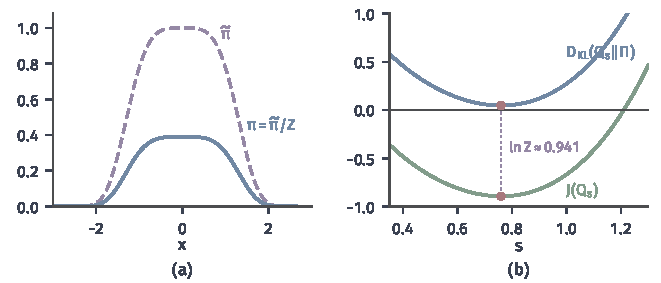
\includegraphics[width=112mm]{figures/07-probability/07-distribution-optimization/matplotlib/dapx-unnormalized/figure.pdf}
 \caption{未归一化目标。(a)$\widetilde{\pi}(x)=\mathrm{e}^{-x^{4}/4}$（紫色虚线）与归一化后的密度$\pi=\widetilde{\pi}/Z$（蓝），$Z\approx2.564$。(b)候选$Q_s=\mathcal{N}(0,s^{2})$：绿线是可计算的$J(Q_s)$，蓝线是$D_{\mathrm{KL}}(Q_s\Vert\Pi)$，两者相差常数$\ln Z\approx0.941$（紫色点线），在同一个$s^{*}=3^{-1/4}\approx0.760$处取最小值（红点）。}
 \label{fig:dapx-unnormalized}
\end{BookInlineFigure}

\paragraph{计算需求}
求$J(Q)$需要对候选$Q$求两个期望：$\ln q$与$\ln\widetilde{\pi}$。前者对高斯、乘积等候选通常有闭式；后者在本例中有闭式，一般情况下可以从$Q$抽样后取平均来估计，误差由第~\ref{chap:monte-carlo-integration-error}章分析。对目标$\Pi$只需要逐点计算$\widetilde{\pi}$，不需要$Z$，不需要从$\Pi$抽样，也不需要任何$\Pi$下的期望。这正是这个方向在目标难以计算时最常用的原因。

\subsection{按目标分布计算KL}
\label{sec:dapx-forward-kl}

第二个问题是
\begin{equation}
 \min_{Q\in\mathcal{Q}}D_{\mathrm{KL}}(\Pi\Vert Q)=\min_{Q\in\mathcal{Q}}\mathbb{E}_{\Pi}\Bigl[\ln\frac{\pi(X)}{q(X)}\Bigr] ,
 \label{eq:dapx-forward-problem}
\end{equation}
相应地常称为\term{正向KL散度}（forward KL divergence）的最小化。现在权重是$\pi$：目标常出现的地方，候选给的概率若太小就要付出代价。

\paragraph{有限的条件}
$D_{\mathrm{KL}}(\Pi\Vert Q)<\infty$要求$\Pi\ll Q$：候选必须覆盖目标有正概率的每个区域。只要漏掉一个这样的区域，KL就是$+\infty$。即使没有完全漏掉，覆盖不足也代价很重。取双峰目标
\begin{equation}
 \pi=0.7\,\mathcal{N}(-2,0.6^{2})+0.3\,\mathcal{N}(2,0.6^{2}) ,
 \label{eq:dapx-bimodal}
\end{equation}
候选$Q=\mathcal{N}(-2,0.6^{2})$只盖住左峰。数值积分给出
\[
 D_{\mathrm{KL}}(Q\Vert\Pi)\approx0.356,\qquad D_{\mathrm{KL}}(\Pi\Vert Q)\approx6.06 .
\]
按候选加权时，候选只看见左峰，在那里它的密度约是目标的$1/0.7$倍，代价约为$-\ln0.7\approx0.357$；按目标加权时，右峰有$0.3$的目标质量落在候选密度只有$\mathrm{e}^{-22}$量级的地方，峰顶处的对数比约为$21$，贡献了绝大部分代价。图~\ref{fig:dapx-weighting}(b)画出两个被积函数。

\begin{BookInlineFigure}
 \centering
 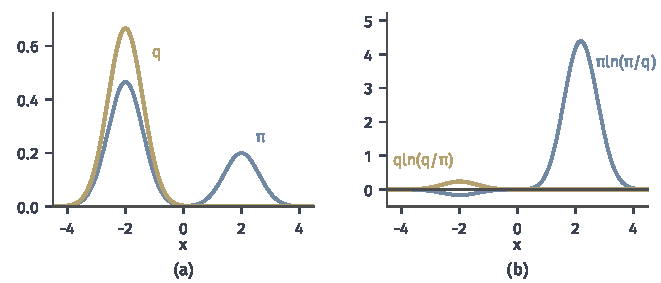
\includegraphics[width=112mm]{figures/07-probability/07-distribution-optimization/matplotlib/dapx-weighting/figure.pdf}
 \caption{两个方向的误差权重。(a)式~\eqref{eq:dapx-bimodal}的双峰目标（蓝）与只覆盖左峰的候选$\mathcal{N}(-2,0.6^{2})$（黄）。(b)被积函数：黄线$q\ln(q/\pi)$只在左峰附近有一个小鼓包，积分约$0.356$；蓝线$\pi\ln(\pi/q)$在右峰处高达$4$以上，积分约$6.06$。}
 \label{fig:dapx-weighting}
\end{BookInlineFigure}

\paragraph{与交叉熵的关系}
在离散情形，第~\ref{chap:information-measures}章已经证明，$H(\Pi)<\infty$时
\[
 D_{\mathrm{KL}}(\Pi\Vert Q)=H(\Pi,Q)-H(\Pi) .
\]
对一般的参考测度，同样的拆分需要两个积分分别有限：设$\mathbb{E}_{\Pi}\lvert\ln\pi(X)\rvert<\infty$与$\mathbb{E}_{\Pi}\lvert\ln q(X)\rvert<\infty$，则可以把对数比的期望拆成两项之差，
\begin{equation}
 D_{\mathrm{KL}}(\Pi\Vert Q)=\mathbb{E}_{\Pi}[\ln\pi(X)]-\mathbb{E}_{\Pi}[\ln q(X)] .
 \label{eq:dapx-forward-split}
\end{equation}
第一项与$Q$无关。于是在满足这两个条件的候选中，最小化正向KL等价于最大化$\mathbb{E}_{\Pi}[\ln q(X)]$，即使交叉熵最小。条件不能省：若$\mathbb{E}_{\Pi}\lvert\ln\pi\rvert=\infty$，式~\eqref{eq:dapx-forward-split}的右边可能是$\infty-\infty$，没有意义，只能回到对数比本身做比较。

式~\eqref{eq:dapx-forward-split}也说明了这个方向的计算需求：要算$\mathbb{E}_{\Pi}[\ln q(X)]$及其关于候选的变化，必须能对目标$\Pi$求期望，或者有从$\Pi$抽得的样本。候选再容易抽样也无济于事，因为平均是按$\Pi$做的。若手头只有未归一化的$\widetilde{\pi}$，这个方向反而无从下手。用样本平均代替$\mathbb{E}_{\Pi}$就是统计中的最大似然，它的统计性质属于卷八，本章只处理$\Pi$下的期望能够计算的情形。

\paragraph{指数族候选：矩匹配}
当候选集合是指数族时，正向KL的最优解有一个简单的刻画。设
\[
 q_{\bm{\theta}}(x)=h(x)\exp\bigl(\langle\bm{\theta},\bm{T}(x)\rangle-A(\bm{\theta})\bigr),\qquad \bm{\theta}\in\Theta ,
\]
是第~\ref{chap:distribution-families}章的正则指数族，$\Theta$是开的自然参数域。由那里的结论，$\bm{T}$在每个$q_{\bm{\theta}}$下各阶矩有限，并且对数配分函数的梯度是均值参数：
\[
 \nabla A(\bm{\theta})=\mathbb{E}_{q_{\bm{\theta}}}[\bm{T}(X)] .
\]
最小化$-\mathbb{E}_{\Pi}[\ln q_{\bm{\theta}}]$时，对$\bm{\theta}$求梯度得到$\nabla A(\bm{\theta})-\mathbb{E}_{\Pi}[\bm{T}]$。这提示最优候选应当与目标有相同的$\bm{T}$的期望。下面的定理把这个提示变成完整的结论，并且不需要拆分式~\eqref{eq:dapx-forward-split}所要求的熵条件。

\begin{theorem}[正向KL与矩匹配]
\label{thm:dapx-moment-matching}
设$\{q_{\bm{\theta}}:\bm{\theta}\in\Theta\}$是上述正则指数族，$\mathbb{E}_{\Pi}\lVert\bm{T}(X)\rVert_2<\infty$。设存在$\bm{\theta}^{*}\in\Theta$使
\begin{equation}
 \mathbb{E}_{q_{\bm{\theta}^{*}}}[\bm{T}(X)]=\mathbb{E}_{\Pi}[\bm{T}(X)] ,
 \label{eq:dapx-moment-match}
\end{equation}
并且$D_{\mathrm{KL}}(\Pi\Vert Q_{\bm{\theta}^{*}})<\infty$。则对每个$\bm{\theta}\in\Theta$，
\begin{equation}
 D_{\mathrm{KL}}(\Pi\Vert Q_{\bm{\theta}})=D_{\mathrm{KL}}(\Pi\Vert Q_{\bm{\theta}^{*}})+D_{\mathrm{KL}}(Q_{\bm{\theta}^{*}}\Vert Q_{\bm{\theta}}) .
 \label{eq:dapx-pythagoras}
\end{equation}
因此$Q_{\bm{\theta}^{*}}$是族内唯一使正向KL最小的分布。
\end{theorem}

\begin{proof}
族中各成员的密度在同一个集合$\{h>0\}$上为正，所以它们相互绝对连续。由$D_{\mathrm{KL}}(\Pi\Vert Q_{\bm{\theta}^{*}})<\infty$知$\Pi\ll Q_{\bm{\theta}^{*}}$，于是$\Pi\ll Q_{\bm{\theta}}$。在$\{h>0\}$上，由密度的链式法则，
\[
 \ln\frac{\pi}{q_{\bm{\theta}}}=\ln\frac{\pi}{q_{\bm{\theta}^{*}}}+\ln\frac{q_{\bm{\theta}^{*}}}{q_{\bm{\theta}}} .
\]
第二项是$\bm{T}$的仿射函数：
\[
 \ln\frac{q_{\bm{\theta}^{*}}(x)}{q_{\bm{\theta}}(x)}=\langle\bm{\theta}^{*}-\bm{\theta},\bm{T}(x)\rangle-A(\bm{\theta}^{*})+A(\bm{\theta}) .
\]
由$\mathbb{E}_{\Pi}\lVert\bm{T}\rVert_2<\infty$，它在$\Pi$下可积；第一项的期望是有限的$D_{\mathrm{KL}}(\Pi\Vert Q_{\bm{\theta}^{*}})$。两项都有有限期望，可以逐项取$\Pi$下的期望。第二项的期望用式~\eqref{eq:dapx-moment-match}换成$Q_{\bm{\theta}^{*}}$下的期望：
\[
 \langle\bm{\theta}^{*}-\bm{\theta},\mathbb{E}_{\Pi}[\bm{T}]\rangle-A(\bm{\theta}^{*})+A(\bm{\theta})
 =\mathbb{E}_{q_{\bm{\theta}^{*}}}\Bigl[\ln\frac{q_{\bm{\theta}^{*}}(X)}{q_{\bm{\theta}}(X)}\Bigr] .
\]
右边就是$D_{\mathrm{KL}}(Q_{\bm{\theta}^{*}}\Vert Q_{\bm{\theta}})$，这里$\bm{T}$在$Q_{\bm{\theta}^{*}}$下可积，因为$\bm{\theta}^{*}$在开的参数域内。两项相加得式~\eqref{eq:dapx-pythagoras}。由Gibbs不等式，第二项非负，且仅当$Q_{\bm{\theta}}=Q_{\bm{\theta}^{*}}$时为零，所以$Q_{\bm{\theta}^{*}}$是唯一的最小者。
\end{proof}

式~\eqref{eq:dapx-pythagoras}像勾股定理：从$\Pi$到族内任一点的“距离”，等于从$\Pi$到最优点的“距离”加上族内两点之间的“距离”。定理要求式~\eqref{eq:dapx-moment-match}有解。若$\mathbb{E}_{\Pi}[\bm{T}]$落在均值参数可取值集合的边界上，族内没有完全匹配的成员，最优解可能不存在；这和第~\ref{chap:distribution-selection}章矩匹配遇到的边界情形相同。

用这个定理可以直接写出几个最优候选。高斯族的$\bm{T}(x)=(x,x^{2})$，匹配均值和二阶矩，也就是匹配均值和方差。式~\eqref{eq:dapx-bimodal}的双峰目标均值为$0.7\cdot(-2)+0.3\cdot2=-0.8$，方差为
\[
 0.6^{2}+\bigl(0.7\cdot4+0.3\cdot4\bigr)-0.8^{2}=0.36+4-0.64=3.72 ,
\]
所以最优高斯候选是$\mathcal{N}(-0.8,3.72)$。$\operatorname{Exp}(1)$目标的最优高斯候选是$\mathcal{N}(1,1)$，此时正向KL为$\tfrac12\ln(2\pi)-\tfrac12\approx0.419$；而按候选加权的方向对它没有任何有限的候选。四次方目标关于原点对称，均值为零，二阶矩为
\[
 \mathbb{E}_{\Pi}[X^{2}]=\frac{2\,\Gamma(3/4)}{\Gamma(1/4)}\approx0.6760 ,
\]
所以最优高斯候选是$\mathcal{N}(0,0.6760)$。它比上一小节按候选加权得到的$\mathcal{N}(0,0.5774)$宽。

\subsection{KL方向的比较}
\label{sec:dapx-direction-compare}

两个方向都在同一个候选集合里挑选，都以同一个目标为准，结果为什么会不同？一个全部概率为正、只有三个状态的例子就足以说明。取目标与单参数候选族
\begin{equation}
 \Pi=\bigl(\tfrac35,\tfrac{3}{10},\tfrac{1}{10}\bigr),\qquad Q_t=(t,\ 1-2t,\ t),\quad 0<t<\tfrac12 .
 \label{eq:dapx-three-point}
\end{equation}
候选要求状态$1$和状态$3$概率相同，而目标在这两个状态上的概率是$0.6$与$0.1$，相差悬殊。候选只有一个自由度，它必须在“两端各给多少”上作出取舍。

\paragraph{按候选加权}
记$f(t)=D_{\mathrm{KL}}(Q_t\Vert\Pi)$。逐项写出：
\[
 f(t)=t\ln\frac{t}{0.6}+(1-2t)\ln\frac{1-2t}{0.3}+t\ln\frac{t}{0.1} .
\]
对$t$求导。每一项$u\ln(u/c)$对$u$的导数是$\ln(u/c)+1$，中间一项的$u=1-2t$还要乘以$-2$；常数$1$在三项中合计$1-2+1=0$，于是
\[
 f'(t)=\ln\frac{t}{0.6}+\ln\frac{t}{0.1}-2\ln\frac{1-2t}{0.3} .
\]
驻点方程比较的是对数概率比：
\begin{equation}
 \tfrac12\Bigl[\ln\frac{q(1)}{\pi(1)}+\ln\frac{q(3)}{\pi(3)}\Bigr]=\ln\frac{q(2)}{\pi(2)} .
 \label{eq:dapx-reverse-stationary}
\end{equation}
两端状态上对数比的平均，要等于中间状态的对数比。

把式~\eqref{eq:dapx-reverse-stationary}写成$t^{2}/(0.6\cdot0.1)=(1-2t)^{2}/0.3^{2}$，取正的平方根，
\[
 \frac{t}{1-2t}=\frac{\sqrt{0.06}}{0.3}=\sqrt{\tfrac23} .
\]
解出
\[
 t_{\mathrm{r}}=\frac{\sqrt{2/3}}{1+2\sqrt{2/3}}=\frac{4-\sqrt6}{5}\approx0.3101 .
\]
又$f''(t)=2/t+4/(1-2t)>0$，$f$是严格凸函数，这个驻点是唯一的最小点。可以看出，按候选加权时两端共享的概率由$\pi(1)$与$\pi(3)$的几何平均$\sqrt{0.06}\approx0.245$决定，再与$\pi(2)=0.3$一起归一化。

\paragraph{按目标加权}
记$g(t)=D_{\mathrm{KL}}(\Pi\Vert Q_t)$。与$t$有关的只有交叉熵部分：
\[
 g(t)=\sum_{k}\pi(k)\ln\pi(k)-0.7\ln t-0.3\ln(1-2t) .
\]
求导得
\[
 g'(t)=-\frac{0.7}{t}+\frac{0.6}{1-2t} .
\]
驻点方程比较的是概率比的倒数，即目标与候选之比：
\begin{equation}
 \tfrac12\Bigl[\frac{\pi(1)}{q(1)}+\frac{\pi(3)}{q(3)}\Bigr]=\frac{\pi(2)}{q(2)} .
 \label{eq:dapx-forward-stationary}
\end{equation}
代入数值，驻点方程是$0.7(1-2t)=0.6t$，解得
\[
 t_{\mathrm{f}}=0.35 .
\]
又$g''(t)=0.7/t^{2}+1.2/(1-2t)^{2}>0$，这也是唯一的最小点。此时两端各得$\pi(1)$与$\pi(3)$的算术平均$0.35$，中间状态的$0.3$与目标完全相同。这正是定理~\ref{thm:dapx-moment-matching}的结论：$Q_t$是统计量$T=\mathbf{1}_{\{X\neq2\}}$生成的指数族，正向KL的最优解匹配$\mathbb{E}[T]=\Pi(X\neq2)=0.7$。

\paragraph{两个解的比较}
两个最优候选为
\[
 Q_{t_{\mathrm{r}}}\approx(0.310,\ 0.380,\ 0.310),\qquad Q_{t_{\mathrm{f}}}=(0.35,\ 0.30,\ 0.35) .
\]
把每个解放到另一个方向上评价，各自都不是最优：
\[
 \begin{aligned}
 D_{\mathrm{KL}}(Q_{t_{\mathrm{r}}}\Vert\Pi)&\approx0.2359, & D_{\mathrm{KL}}(Q_{t_{\mathrm{f}}}\Vert\Pi)&\approx0.2498,\\
 D_{\mathrm{KL}}(\Pi\Vert Q_{t_{\mathrm{r}}})&\approx0.2121, & D_{\mathrm{KL}}(\Pi\Vert Q_{t_{\mathrm{f}}})&\approx0.1981 .
 \end{aligned}
\]
差别的来源在状态$3$与状态$1$。状态$3$的目标概率只有$0.1$，候选给它$t\geq0.31$：按候选加权时这一项是$t\ln(t/0.1)$，权重大、对数比也大，所以$t$被压低，多出的概率转给中间状态。状态$1$的目标概率是$0.6$，候选只给$t\leq0.35$：按目标加权时这一项是$0.6\ln(0.6/t)$，权重是$0.6$，所以$t$被抬高。

\begin{BookInlineFigure}
 \centering
 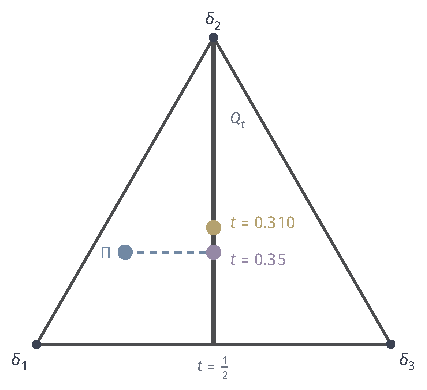
\includegraphics[width=72mm]{figures/07-probability/07-distribution-optimization/tikz/dapx-simplex-segment/figure.pdf}
 \caption{三状态概率表组成的三角形，顶点$\delta_k$是集中在状态$k$的分布，一点到三边的远近给出三个概率。蓝点是目标$\Pi=(0.6,0.3,0.1)$，深灰粗线是候选族$Q_t$（从$\delta_2$到底边中点）。黄点是按候选加权的最优解$t=0.310$，紫点是按目标加权的最优解$t=0.35$，它与$\Pi$等高，即中间状态的概率同为$0.3$。}
 \label{fig:dapx-simplex-segment}
\end{BookInlineFigure}

图~\ref{fig:dapx-simplex-segment}把这件事放在概率单纯形里：候选族是一条线段，目标在线段之外，两个方向在线段上选了不同的点。图~\ref{fig:dapx-three-point}画出两条目标曲线和三个分布的概率。两条曲线都是凸的，最低点相距$0.04$；概率图中，黄色候选把多出的概率放在中间状态，紫色候选保持中间状态与目标一致。

\begin{BookInlineFigure}
 \centering
 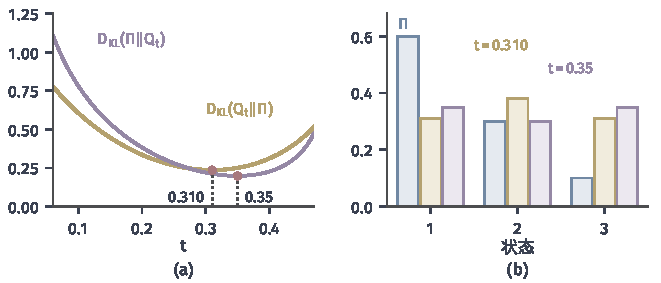
\includegraphics[width=112mm]{figures/07-probability/07-distribution-optimization/matplotlib/dapx-three-point/figure.pdf}
 \caption{三状态例子的两个方向。(a)$D_{\mathrm{KL}}(Q_t\Vert\Pi)$（黄）与$D_{\mathrm{KL}}(\Pi\Vert Q_t)$（紫）随$t$的变化，红点是最小点$t=0.310$与$t=0.35$。(b)目标$\Pi$（蓝）与两个最优候选（黄：$t=0.310$；紫：$t=0.35$）在三个状态上的概率。}
 \label{fig:dapx-three-point}
\end{BookInlineFigure}

\paragraph{择峰与覆盖}
目标有几个分离的峰而候选只有一个峰时，两个方向的差别最明显。式~\eqref{eq:dapx-bimodal}的双峰目标用高斯族逼近：按目标加权的最优解是矩匹配的$\mathcal{N}(-0.8,3.72)$，它横跨两个峰，在两峰之间目标几乎没有质量的地方放了很多概率，KL约为$0.558$；按候选加权的目标函数有两个局部最小点，分别贴住一个峰，值约为$0.356$与$1.202$，接近$-\ln0.7$与$-\ln0.3$。图~\ref{fig:dapx-bimodal-fits}(b)对每个均值$m$先把$s$取到最优，画出两个目标随$m$的变化。

\begin{BookInlineFigure}
 \centering
 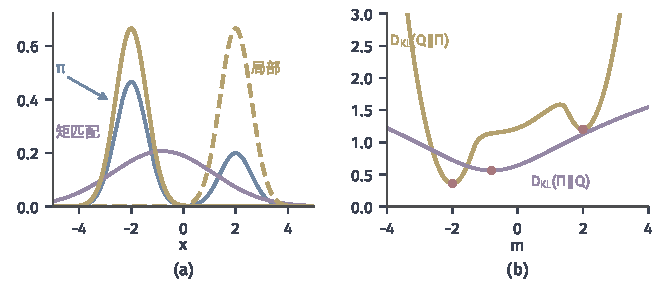
\includegraphics[width=112mm]{figures/07-probability/07-distribution-optimization/matplotlib/dapx-bimodal-fits/figure.pdf}
 \caption{用单个高斯逼近双峰目标。(a)目标（蓝）；按目标加权的最优解$\mathcal{N}(-0.8,3.72)$（紫，矩匹配）；按候选加权的两个局部最优解$\mathcal{N}(-2,0.6^{2})$（黄实线）与$\mathcal{N}(2,0.6^{2})$（黄虚线）。(b)固定均值$m$、把标准差$s$取到最优后的目标值：黄线是$D_{\mathrm{KL}}(Q\Vert\Pi)$，在$m=\pm2$附近各有一个局部最小（$0.356$与$1.202$）；紫线是$D_{\mathrm{KL}}(\Pi\Vert Q)$，只有一个最小点$m=-0.8$（$0.558$）。}
 \label{fig:dapx-bimodal-fits}
\end{BookInlineFigure}

按候选加权的方向倾向于选中目标的一个峰而忽略其他峰，称为\term{择峰}（mode seeking）；按目标加权的方向倾向于把目标所有有质量的区域都盖住，称为\term{质量覆盖}（mass covering）。这两个说法描述的是倾向，不是定理，是否出现要看目标与候选集合的具体形状。三状态例子里没有分离的峰，两个最优解都把正概率给了每个状态，按候选加权的解也没有“择”出哪一个状态，只是把概率从小概率的一端挪到了中间。能下结论的只有本节算出的这些事实：权重来自哪个分布，支持条件落在哪一边，驻点方程比较的是对数比还是比值本身。

\section{平均场逼近}
\label{sec:dapx-mean-field}

高维目标难算，往往是因为各分量纠缠在一起：求一个分量的边缘，要对其余所有分量的联合取值求和。如果候选分布让各分量独立，很多计算就拆成了一维的计算。把变量分成$m$组$\bm{x}=(x_1,\dots,x_m)$，$x_j\in\mathcal{X}_j$（每组可以是一个分量，也可以是几个分量），参考测度取各组参考测度的乘积，候选限制为
\begin{equation}
 q(\bm{x})=\prod_{j=1}^{m}q_j(x_j) ,
 \label{eq:dapx-product}
\end{equation}
其中每个因子$q_j$可以是$\mathcal{X}_j$上任意一个概率密度。用这种乘积分布逼近目标，称为\term{平均场逼近}（mean-field approximation）。名称来自统计物理：每个分量感受到的是其余分量的平均作用，下一小节的更新公式正是如此。

这里的限制只有一条：组与组之间独立。每个因子本身不限于任何参数族，可以是任意形状。所以“乘积”与“有限维参数化”是两回事：前者限制的是依赖结构，后者限制的是每个分布的形状。本节先看独立性限制本身的后果，再推导按候选加权的方向下逐个因子求最优的更新。

先处理比较简单的一个方向。按目标加权时，最优的乘积分布就是目标的边缘乘积，并且最小值正是第~\ref{chap:information-measures}章的互信息。

\begin{lemma}[正向KL下的最优乘积]
\label{lem:dapx-forward-product}
设$m=2$，目标$\Pi$有边缘$\Pi_1,\Pi_2$，且互信息有限：
\begin{equation}
 I(X_1;X_2)=D_{\mathrm{KL}}(\Pi\Vert\Pi_1\otimes\Pi_2)<\infty .
 \label{eq:dapx-mi-finite}
\end{equation}
则对任意因子$Q_1,Q_2$，
\begin{equation}
 D_{\mathrm{KL}}(\Pi\Vert Q_1\otimes Q_2)=I(X_1;X_2)+D_{\mathrm{KL}}(\Pi_1\Vert Q_1)+D_{\mathrm{KL}}(\Pi_2\Vert Q_2) .
 \label{eq:dapx-forward-product}
\end{equation}
因此最优乘积唯一，是$\Pi_1\otimes\Pi_2$，最小值是$I(X_1;X_2)$。
\end{lemma}

\begin{proof}
若$\Pi_1\not\ll Q_1$，则有集合$A$使$\Pi_1(A)>0=Q_1(A)$，于是
\[
 \Pi(A\times\mathcal{X}_2)>0=(Q_1\otimes Q_2)(A\times\mathcal{X}_2) ,
\]
两边都是$+\infty$；$\Pi_2\not\ll Q_2$同理。下设$\Pi_j\ll Q_j$，密度记为$\pi_j,q_j$。由$I<\infty$知$\Pi\ll\Pi_1\otimes\Pi_2$，于是$\Pi\ll Q_1\otimes Q_2$，并且在$\Pi$几乎处处成立
\[
 \ln\frac{\pi(x_1,x_2)}{q_1(x_1)q_2(x_2)}=\ln\frac{\pi(x_1,x_2)}{\pi_1(x_1)\pi_2(x_2)}+\ln\frac{\pi_1(x_1)}{q_1(x_1)}+\ln\frac{\pi_2(x_2)}{q_2(x_2)} .
\]
第一项的期望是有限的$I$。后两项只依赖一个变量，在$\Pi$下的期望等于在边缘下的期望，分别是$D_{\mathrm{KL}}(\Pi_j\Vert Q_j)\in[0,+\infty]$，它们的负部都可积。三项的负部都可积，期望可以逐项相加，得到式~\eqref{eq:dapx-forward-product}。后两项非负，且仅在$Q_j=\Pi_j$时为零。
\end{proof}

对上一节的概率表~\eqref{eq:dapx-table}，引理给出最优乘积是四格各$0.25$的均匀表，最小值$I(X_1;X_2)\approx0.3681$。多于两组时，同样的拆分给出最优乘积仍是各组边缘的乘积，最小值是目标与边缘乘积之间的KL。这个方向的计算需求也一目了然：需要目标的各个边缘，而求边缘往往正是困难所在。

\subsection{独立性限制的影响}
\label{sec:dapx-independence}

乘积限制会改变哪些数值特征？用一个能完整算出两个方向的例子来看。目标是均值为零、两个分量方差都是$1$、相关系数为$\rho$的二维高斯分布，
\begin{equation}
 \Pi=\mathcal{N}(\bm{0},\bm{\Sigma}),\qquad \bm{\Sigma}=\begin{bmatrix}1&\rho\\\rho&1\end{bmatrix},\qquad 0<\lvert\rho\rvert<1 .
 \label{eq:dapx-gauss-target}
\end{equation}
候选是独立的高斯分布
\[
 Q=\mathcal{N}(m_1,s_1^{2})\otimes\mathcal{N}(m_2,s_2^{2}) ,
\]
即均值为$\bm{m}=(m_1,m_2)$、协方差矩阵为$\bm{S}=\operatorname{diag}(s_1^{2},s_2^{2})$的高斯分布。需要用到精度矩阵
\[
 \bm{\Sigma}^{-1}=\frac{1}{1-\rho^{2}}\begin{bmatrix}1&-\rho\\-\rho&1\end{bmatrix},\qquad \det\bm{\Sigma}=1-\rho^{2} .
\]

\paragraph{按候选加权}
目标的对数密度是
\[
 \ln\pi(\bm{x})=-\ln(2\pi)-\tfrac12\ln(1-\rho^{2})-\tfrac12\bm{x}^{\top}\bm{\Sigma}^{-1}\bm{x} .
\]
在$Q$下，二次型的期望等于协方差部分加均值部分：
\[
 \mathbb{E}_{Q}\bigl[\bm{X}^{\top}\bm{\Sigma}^{-1}\bm{X}\bigr]=\operatorname{tr}(\bm{\Sigma}^{-1}\bm{S})+\bm{m}^{\top}\bm{\Sigma}^{-1}\bm{m}=\frac{s_1^{2}+s_2^{2}}{1-\rho^{2}}+\bm{m}^{\top}\bm{\Sigma}^{-1}\bm{m} .
\]
候选自身的对数密度期望是两个一维高斯负熵之和，$-\ln(2\pi)-\ln s_1-\ln s_2-1$。相减得
\[
 D_{\mathrm{KL}}(Q\Vert\Pi)=-\ln s_1-\ln s_2-1+\tfrac12\ln(1-\rho^{2})+\frac{s_1^{2}+s_2^{2}}{2(1-\rho^{2})}+\tfrac12\bm{m}^{\top}\bm{\Sigma}^{-1}\bm{m} .
\]

$\bm{\Sigma}^{-1}$正定，均值项在$\bm{m}=\bm{0}$时最小。对$s_1$求导并令其为零，
\[
 -\frac{1}{s_1}+\frac{s_1}{1-\rho^{2}}=0,\qquad s_1^{2}=1-\rho^{2} ,
\]
$s_2$相同。代回，最小值为
\begin{equation}
 \min_{Q}D_{\mathrm{KL}}(Q\Vert\Pi)=-\ln(1-\rho^{2})-1+\tfrac12\ln(1-\rho^{2})+1=-\tfrac12\ln(1-\rho^{2}) .
 \label{eq:dapx-gauss-reverse}
\end{equation}
最优因子的方差$1-\rho^{2}$不是目标的边缘方差$1$，而是给定另一个分量后的条件方差，也是精度矩阵对角元的倒数$1/(\bm{\Sigma}^{-1})_{1,1}$。

\paragraph{按目标加权}
由引理~\ref{lem:dapx-forward-product}，最优乘积是两个边缘$\mathcal{N}(0,1)$的乘积。最小值是高斯分布的互信息：
\[
 \begin{aligned}
 I(X_1;X_2)&=\mathbb{E}_{\Pi}\bigl[\ln\pi-\ln\pi_1-\ln\pi_2\bigr]\\
 &=-\tfrac12\ln(1-\rho^{2})+\tfrac12\,\mathbb{E}_{\Pi}\bigl[X_1^{2}+X_2^{2}-\bm{X}^{\top}\bm{\Sigma}^{-1}\bm{X}\bigr] .
 \end{aligned}
\]
$\bm{X}\sim\mathcal{N}(\bm{0},\bm{\Sigma})$时，方括号中两部分的期望相等：
\[
 \mathbb{E}\bigl[\bm{X}^{\top}\bm{\Sigma}^{-1}\bm{X}\bigr]=\operatorname{tr}(\bm{\Sigma}^{-1}\bm{\Sigma})=2,\qquad \mathbb{E}\bigl[X_1^{2}+X_2^{2}\bigr]=2 .
\]
所以
\begin{equation}
 \min_{Q}D_{\mathrm{KL}}(\Pi\Vert Q)=I(X_1;X_2)=-\tfrac12\ln(1-\rho^{2}) .
 \label{eq:dapx-gauss-forward}
\end{equation}

\paragraph{两个方向的比较}
取$\rho=0.8$。两个方向的最小值相同，都是$-\tfrac12\ln0.36\approx0.5108$，选出的分布却不同：
\[
 Q_{\mathrm{r}}=\mathcal{N}(\bm{0},0.36\,\bm{I}_2),\qquad Q_{\mathrm{f}}=\mathcal{N}(\bm{0},\bm{I}_2) .
\]
两者都把协方差删成了零，这是乘积限制本身的后果，与方向无关。区别在于分量的方差：按候选加权得到$0.36$，标准差$0.6$；按目标加权保持了$1$。图~\ref{fig:dapx-gauss-meanfield}(a)中，蓝色的目标椭圆沿对角线拉长；黄色圆被压在椭圆最窄的方向里，整个落在目标的高概率区域中；紫色虚线圆则与目标的边缘一致，但伸进了椭圆两侧目标概率很低的角落。

\begin{BookInlineFigure}
 \centering
 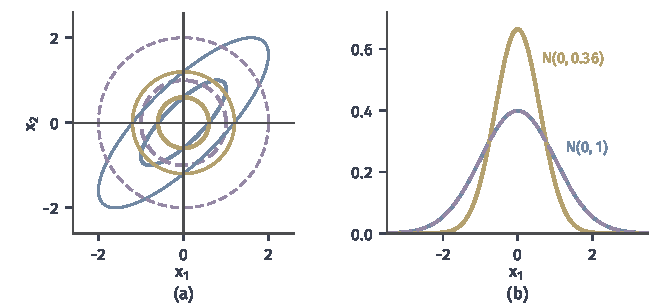
\includegraphics[width=112mm]{figures/07-probability/07-distribution-optimization/matplotlib/dapx-gauss-meanfield/figure.pdf}
 \caption{独立高斯候选逼近相关高斯目标，$\rho=0.8$。(a)等高线$\bm{x}^{\top}\bm{C}^{-1}\bm{x}=c^{2}$，$c=1,2$：目标$\bm{C}=\bm{\Sigma}$（蓝）；按候选加权的最优解$\bm{C}=0.36\,\bm{I}_2$（黄）；按目标加权的最优解$\bm{C}=\bm{I}_2$（紫色虚线）。(b)$X_1$的边缘密度：目标与按目标加权的解都是$\mathcal{N}(0,1)$（蓝线与紫色虚线重合），按候选加权的解是$\mathcal{N}(0,0.36)$（黄）。}
 \label{fig:dapx-gauss-meanfield}
\end{BookInlineFigure}

方差变小会直接影响尾概率。事件$\{\lvert X_1\rvert>1.5\}$在目标与$Q_{\mathrm{r}}$下的概率分别是
\[
 2\bigl(1-\Phi(1.5)\bigr)\approx0.134,\qquad 2\bigl(1-\Phi(1.5/0.6)\bigr)=2\bigl(1-\Phi(2.5)\bigr)\approx0.0124 ,
\]
后者小了十倍以上。所以，即使是族内最优的近似，也可能改变后续任务关心的数值特征；KL的值$0.51$本身不会告诉我们这一点。

把一个方向的最优解放到另一个方向上评价，两者都明显变差。代入上面的公式，
\[
 D_{\mathrm{KL}}(\Pi\Vert Q_{\mathrm{r}})=D_{\mathrm{KL}}(Q_{\mathrm{f}}\Vert\Pi)=\tfrac12\Bigl[\frac{2\rho^{2}}{1-\rho^{2}}+\ln(1-\rho^{2})\Bigr]\approx1.267 .
\]
图~\ref{fig:dapx-rho-curves}画出这些量随$\rho$的变化。$\rho\to\pm1$时，两个变量越来越接近同一个变量，乘积候选能做到的最好程度$-\tfrac12\ln(1-\rho^{2})$趋于无穷，按候选加权所得的方差$1-\rho^{2}$趋于零。

\begin{BookInlineFigure}
 \centering
 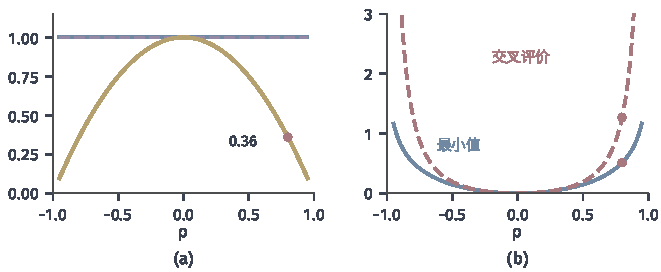
\includegraphics[width=112mm]{figures/07-probability/07-distribution-optimization/matplotlib/dapx-rho-curves/figure.pdf}
 \caption{相关系数的影响。(a)最优独立候选的分量方差：按候选加权为$1-\rho^{2}$（黄），按目标加权为$1$（紫色虚线，与目标边缘方差的蓝线重合）；红点是$\rho=0.8$时的$0.36$。(b)蓝线是两个方向共同的最小值$-\tfrac12\ln(1-\rho^{2})$；红色虚线是交叉评价，即一个方向的最优解在另一个方向上的值。}
 \label{fig:dapx-rho-curves}
\end{BookInlineFigure}

概率表~\eqref{eq:dapx-table}上也有同样的现象，只是形式不同。下一小节将求出，按候选加权的最优乘积是$q_1=q_2=(\tfrac14,\tfrac34)$或$q_1=q_2=(\tfrac34,\tfrac14)$，KL约为$0.4978$，而按目标加权的最优乘积是均匀表。前者让$Q(X_1=X_2)=\tfrac{10}{16}=0.625$，比均匀表的$0.5$更接近目标的$0.9$，代价是把边缘从$\tfrac12$改成了$\tfrac34$。两个方向在同一个乘积限制下各保留了目标的一部分特征，没有一个能全部保留。

\subsection{逐因子的坐标更新}
\label{sec:dapx-cavi}

按候选加权的方向在高斯例子里能直接求解，一般目标则不能。不过乘积结构给了一个好办法：固定其余因子，只调整一个因子，这个子问题有显式的最优解。依次对每个因子这样做，就是\term{坐标上升变分推断}（coordinate ascent variational inference），简称CAVI。“上升”指的是对$\ln Z$的变分下界~\eqref{eq:dapx-lower-bound}上升，等价于对KL下降。

\paragraph{主要思想}
固定$q_k$（$k\neq j$），把它们的乘积记为$q_{-j}$，对应的变量记为$\bm{x}_{-j}$。目标对数密度对$x_j$的依赖，在候选看来是什么样子？最自然的答案是：对其余变量按$q_{-j}$求平均。定义
\begin{equation}
 g_j(x_j)=\mathbb{E}_{q_{-j}}\bigl[\ln\widetilde{\pi}(x_j,\bm{X}_{-j})\bigr] .
 \label{eq:dapx-cavi-g}
\end{equation}
它是在“其余变量服从当前因子”的假定下，$x_j$处目标的平均对数密度。把它取指数并归一化，得到当前因子的更新：
\begin{equation}
 q_j^{\mathrm{new}}(x_j)=\frac{\exp(g_j(x_j))}{\int_{\mathcal{X}_j}\exp(g_j)\,\mathrm{d}\lambda_j} .
 \label{eq:dapx-cavi-update}
\end{equation}
下面的定理说明它恰好是子问题的唯一最优解。先在有限状态、目标处处为正的情形证明，这时所有求和都是有限和，没有可积性问题。

\begin{theorem}[逐因子最优更新]
\label{thm:dapx-cavi}
设每个$\mathcal{X}_k$是有限集，$\widetilde{\pi}(\bm{x})>0$对一切$\bm{x}$成立。固定$q_k$（$k\neq j$），按式~\eqref{eq:dapx-cavi-g}、\eqref{eq:dapx-cavi-update}定义$g_j$与$q_j^{\mathrm{new}}$。则对$\mathcal{X}_j$上任意概率$q_j$，
\begin{equation}
 D_{\mathrm{KL}}(q_j\otimes q_{-j}\Vert\Pi)=D_{\mathrm{KL}}(q_j\Vert q_j^{\mathrm{new}})+c_j ,
 \label{eq:dapx-cavi-identity}
\end{equation}
其中$c_j$只依赖$q_{-j}$与$\widetilde{\pi}$。因此$q_j^{\mathrm{new}}$是固定其余因子时唯一的最优因子。
\end{theorem}

\begin{proof}
记$Q=q_j\otimes q_{-j}$。由式~\eqref{eq:dapx-J-shift}，$D_{\mathrm{KL}}(Q\Vert\Pi)=J(Q)+\ln Z$，只需处理$J(Q)$。乘积分布的对数密度是各因子对数密度之和，所以
\[
 \mathbb{E}_{Q}[\ln q(\bm{X})]=\sum_{x_j}q_j(x_j)\ln q_j(x_j)+\sum_{k\neq j}\sum_{x_k}q_k(x_k)\ln q_k(x_k) .
\]
目标对数密度的期望先对$\bm{x}_{-j}$求和、再对$x_j$求和，由式~\eqref{eq:dapx-cavi-g}，
\[
 \mathbb{E}_{Q}[\ln\widetilde{\pi}(\bm{X})]=\sum_{x_j}q_j(x_j)\sum_{\bm{x}_{-j}}q_{-j}(\bm{x}_{-j})\ln\widetilde{\pi}(x_j,\bm{x}_{-j})=\sum_{x_j}q_j(x_j)g_j(x_j) .
\]

记$Z_j=\sum_{x_j}\exp(g_j(x_j))$，则$g_j(x_j)=\ln q_j^{\mathrm{new}}(x_j)+\ln Z_j$。两式相减，并把与$q_j$无关的项合并：
\[
 J(Q)=\sum_{x_j}q_j(x_j)\ln\frac{q_j(x_j)}{q_j^{\mathrm{new}}(x_j)}-\ln Z_j+\sum_{k\neq j}\sum_{x_k}q_k(x_k)\ln q_k(x_k) .
\]
第一项是$D_{\mathrm{KL}}(q_j\Vert q_j^{\mathrm{new}})$，其余各项不含$q_j$。加上$\ln Z$即得式~\eqref{eq:dapx-cavi-identity}，其中
\[
 c_j=-\ln Z_j+\sum_{k\neq j}\sum_{x_k}q_k(x_k)\ln q_k(x_k)+\ln Z .
\]
由Gibbs不等式，第一项非负，仅在$q_j=q_j^{\mathrm{new}}$时为零。
\end{proof}

更新公式有几处值得注意。第一，用$\widetilde{\pi}$还是$\pi$不影响结果：两者只差常数$\ln Z$，$g_j$随之平移一个常数，取指数归一化后抵消。第二，$\widetilde{\pi}(x_j,\bm{x}_{-j})$是条件密度$\pi(x_j\mid\bm{x}_{-j})$乘以一个不含$x_j$的因子，所以$q_j^{\mathrm{new}}$也正比于$\exp\bigl(\mathbb{E}_{q_{-j}}[\ln\pi(x_j\mid\bm{X}_{-j})]\bigr)$：它是目标条件分布在其余因子下的“对数平均”。这是名称中“平均场”的来源：$x_j$看到的不是其余变量的真实取值，而是它们在当前候选下的平均影响。第三，更新只用到$\ln\widetilde{\pi}$的期望，对目标只需要逐点计算未归一化密度。图~\ref{fig:dapx-factor-update}用概率表~\eqref{eq:dapx-table}演示一次更新。

\begin{BookInlineFigure}
 \centering
 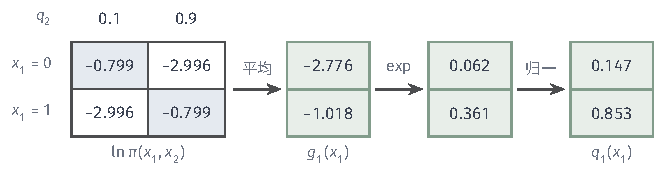
\includegraphics[width=112mm]{figures/07-probability/07-distribution-optimization/tikz/dapx-factor-update/figure.pdf}
 \caption{一次因子更新。左：目标对数概率$\ln\pi(x_1,x_2)$，列上方是当前因子$q_2=(0.1,0.9)$。按$q_2$对每一行加权平均得到$g_1(x_1)$（式~\eqref{eq:dapx-cavi-g}），取指数后归一化，得到新的$q_1=(0.147,0.853)$（式~\eqref{eq:dapx-cavi-update}）。}
 \label{fig:dapx-factor-update}
\end{BookInlineFigure}

\paragraph{高斯目标}
对式~\eqref{eq:dapx-gauss-target}的目标，记精度矩阵$\bm{\Lambda}=\bm{\Sigma}^{-1}$，取未归一化密度
\[
 \ln\widetilde{\pi}(\bm{x})=-\tfrac12\bm{x}^{\top}\bm{\Lambda}\bm{x} .
\]
固定$q_2$，记它的均值为$m_2$。展开二次型，对$X_2$求期望，只保留含$x_1$的项：
\[
 g_1(x_1)=-\tfrac12\Lambda_{1,1}x_1^{2}-\Lambda_{1,2}x_1m_2+\text{常数} .
\]
这是$x_1$的二次函数，取指数后正是高斯密度，配方得到
\[
 q_1^{\mathrm{new}}=\mathcal{N}\Bigl(-\frac{\Lambda_{1,2}}{\Lambda_{1,1}}m_2,\ \frac{1}{\Lambda_{1,1}}\Bigr)=\mathcal{N}\bigl(\rho m_2,\ 1-\rho^{2}\bigr) .
\]
因子是高斯分布这一点不是事先假定的，而是更新公式推出来的；方差$1-\rho^{2}$与上一小节一致，并且不随$q_2$改变。均值的更新是$m_1\leftarrow\rho m_2$，对第二个因子同样有$m_2\leftarrow\rho m_1$。一轮下来$m_2$乘以$\rho^{2}$，从$(m_1,m_2)=(-1.5,2)$出发，第一轮得到$m_1=1.6$，$m_2=1.28$，此后每轮缩小到$0.64$倍，收敛到唯一的最优解$\bm{m}=\bm{0}$。图~\ref{fig:dapx-cavi-gauss}画出这条阶梯形路径。

\begin{BookInlineFigure}
 \centering
 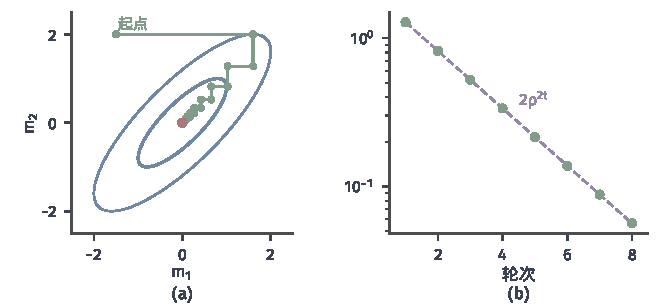
\includegraphics[width=112mm]{figures/07-probability/07-distribution-optimization/matplotlib/dapx-cavi-gauss/figure.pdf}
 \caption{高斯目标上的逐因子更新，$\rho=0.8$。(a)目标等高线（蓝）与因子均值$(m_1,m_2)$的路径（绿）：每步只沿一个坐标方向移动，起点$(-1.5,2)$，红点是最优解$\bm{0}$。(b)每轮结束时的$\lvert m_2\rvert$（绿点，对数纵轴）落在直线$2\rho^{2t}$（紫色虚线）上。}
 \label{fig:dapx-cavi-gauss}
\end{BookInlineFigure}

阶梯的每一步都很短，是因为目标沿对角线拉长：每次只能沿一个坐标轴移动，而沿坐标轴方向目标的“谷”很窄。$\lvert\rho\rvert$越接近$1$，谷越窄，每轮缩小的倍数$\rho^{2}$越接近$1$，收敛越慢。

\paragraph{一般密度}
离开有限状态，定理~\ref{thm:dapx-cavi}的推导需要以下条件，才能让每一步都是有限量的加减：
\begin{itemize}
 \item 对$\lambda_j$几乎处处的$x_j$，$\ln\widetilde{\pi}(x_j,\cdot)$在$q_{-j}$下可积，使$g_j$有定义；
 \item $0<\int\exp(g_j)\,\mathrm{d}\lambda_j<\infty$，使式~\eqref{eq:dapx-cavi-update}能够归一化；
 \item 各因子的$\mathbb{E}_{q_k}\lvert\ln q_k\rvert$有限，$\ln\widetilde{\pi}$在$q_j\otimes q_{-j}$下可积，使Fubini定理允许先对$\bm{x}_{-j}$、再对$x_j$积分。
\end{itemize}
这些条件成立时，证明中的求和换成积分，逐行照搬即可。条件不是形式上的：在高斯目标中，若当前的$q_2$是Cauchy分布，$\mathbb{E}_{q_2}[X_2]$与$\mathbb{E}_{q_2}[X_2^{2}]$都不存在，$g_1$根本没有定义。这时候选的KL也是无穷大，所以实际计算中应当从一个目标值有限的乘积出发，并逐步检查每次更新后上述积分仍然有限。

\paragraph{计算过程}
下面用概率表~\eqref{eq:dapx-table}完整走一遍。两个因子都是$\{0,1\}$上的分布，记$a=q_1(1)$，$b=q_2(1)$。

\needspace{6\baselineskip}
\paragraph{变量}
\begin{itemize}
 \item $\bm{L}\in\mathbb{R}^{2\times2}$：目标对数密度表$L_{x_1,x_2}=\ln\widetilde{\pi}(x_1,x_2)$，只读。
 \item $q_1,q_2$：两个因子，各是长度为$2$的概率向量，在原处更新；二值时只需存$a,b$。
 \item $g$：长度为$2$的工作向量，存放当前正在更新的因子的$g_j$。
 \item $D^{(t)}$：第$t$轮结束时的目标值，用于停止判断；$\varepsilon>0$为容差。
\end{itemize}

\paragraph{初始化}
读入$\bm{L}$，给出第二个因子的初值$q_2^{(0)}$，第一个因子可以任取（它会在第一步被覆盖，只用于计算初始目标值）。例中
\[
 L_{0,0}=L_{1,1}=\ln0.45\approx-0.7985,\qquad L_{0,1}=L_{1,0}=\ln0.05\approx-2.9957 ,
\]
取$q_2^{(0)}=(0.1,\ 0.9)$，$q_1^{(0)}=(0.5,\ 0.5)$，初始目标值$D^{(0)}\approx0.8789$；取$\varepsilon=10^{-4}$。

\needspace{6\baselineskip}
\paragraph{每轮更新}
第$t$轮依次执行：
\begin{enumerate}
 \item \textbf{更新第一个因子。}按式~\eqref{eq:dapx-cavi-g}对每一行用$q_2$加权：
 \[
  g(x_1)=\sum_{x_2}q_2(x_2)L_{x_1,x_2} .
 \]
 再按式~\eqref{eq:dapx-cavi-update}取指数并归一化。数值上先减去$\max g$再取指数，避免下溢。二值时归一化化简为一个logistic函数：
 \[
  a=\frac{1}{1+\exp\bigl(-(g(1)-g(0))\bigr)} .
 \]
 例中第一轮
 \[
  g(0)=0.1\cdot(-0.7985)+0.9\cdot(-2.9957)=-2.7760 ,
 \]
 \[
  g(1)=0.1\cdot(-2.9957)+0.9\cdot(-0.7985)=-1.0182 ,
 \]
 两者之差为$1.7578$，于是
 \[
  a=\frac{1}{1+\mathrm{e}^{-1.7578}}=0.8529,\qquad q_1=(0.1471,\ 0.8529) .
 \]
 这一步后目标值降到$0.5341$。

 \item \textbf{更新第二个因子。}对每一列用新的$q_1$加权：
 \[
  g(x_2)=\sum_{x_1}q_1(x_1)L_{x_1,x_2} ,
 \]
 再取指数并归一化。例中第一轮$2a-1=0.7058$，两个对数概率之差为$\ln0.45-\ln0.05=\ln9=2.1972$，
 \[
  g(1)-g(0)=(2a-1)\ln9=0.7058\cdot2.1972=1.5508 ,
 \]
 于是
 \[
  b=\frac{1}{1+\mathrm{e}^{-1.5508}}=0.8250 .
 \]

 \item \textbf{计算目标值。}乘积分布有四个格，直接求和：
 \[
  D^{(t)}=\sum_{x_1,x_2}q_1(x_1)q_2(x_2)\ln\frac{q_1(x_1)q_2(x_2)}{\pi(x_1,x_2)} .
 \]
 目标只有未归一化形式时改算$J$，停止判断只用差值，不受$\ln Z$影响。例中第一轮$D^{(1)}=0.5117$。

 \item \textbf{停止。}若$D^{(t-1)}-D^{(t)}<\varepsilon$，或已做满预定轮数，输出当前的$q_1,q_2$；否则令$t\leftarrow t+1$，回到第1步。

 例中后续各轮为
 \[
  \begin{array}{cccc}
  t & a & b & D^{(t)}\\
  2 & 0.8067 & 0.7937 & 0.50129\\
  3 & 0.7843 & 0.7772 & 0.49896\\
  4 & 0.7717 & 0.7675 & 0.49824\\
  5 & 0.7641 & 0.7614 & 0.49798\\
  6 & 0.7593 & 0.7576 & 0.49787\\
  7 & 0.7562 & 0.7551 & 0.49783
  \end{array}
 \]
 第$7$轮的下降量$4.3\times10^{-5}$小于$\varepsilon$，停止。
\end{enumerate}

最终得到$q_1\approx(0.244,\ 0.756)$，$q_2\approx(0.245,\ 0.755)$，目标值$0.49783$。继续迭代，$a,b$都趋于$\tfrac34$：二值时更新是$a=\sigma\bigl((2b-1)\ln9\bigr)$，其中$\sigma(z)=1/(1+\mathrm{e}^{-z})$，代入$b=\tfrac34$得$\sigma(\tfrac12\ln9)=\sigma(\ln3)=\tfrac34$，所以$a=b=\tfrac34$是不动点，对应的乘积分布
\[
 Q^{*}=\begin{bmatrix}\tfrac{1}{16}&\tfrac{3}{16}\\\tfrac{3}{16}&\tfrac{9}{16}\end{bmatrix},\qquad D_{\mathrm{KL}}(Q^{*}\Vert\Pi)\approx0.4978 .
\]
停止时的目标值已经与极限相差不到$10^{-4}$，因子却还差约$0.006$：目标值在最优点附近对因子的变化不敏感，用目标值的下降量作停止准则时，因子的精度要另外判断。

\paragraph{收敛与最优性}
由式~\eqref{eq:dapx-cavi-identity}，每次更新一个因子，目标值都不会增加；目标值有下界$0$，所以目标值序列收敛。这是本算法唯一无条件成立的结论。下面三件事要分开看。

第一，目标值收敛不等于因子收敛。在有限状态、各因子始终严格为正的情形，更新映射连续，每个子问题有唯一解，这类分块下降方法的极限点都是驻点；一般情形下需要的条件见\BookChapterRef{chap:block-optimization}{卷五第12章“分块优化”}。

第二，驻点不一定是最小点。从$b^{(0)}=\tfrac12$出发，第一步得到$a=\sigma(0)=\tfrac12$，之后永远停在均匀表，目标值$0.5108$。这是一个鞍点：沿$a=b$方向离开它，目标值下降。

第三，局部最优不一定是全局最优。目标值作为$(a,b)$的函数，对每个坐标单独是凸的（式~\eqref{eq:dapx-cavi-identity}右边是$q_j$的凸函数），但对两个坐标合起来不是凸的。本例有两个最小点$(\tfrac14,\tfrac14)$与$(\tfrac34,\tfrac34)$，从$b^{(0)}=0.2$出发会走到前者。这里两个最小点由对称性给出相同的值；目标不对称时，不同的局部最小点的值一般不同，迭代停在哪里取决于初值。图~\ref{fig:dapx-cavi-table}画出目标值的等高线与两条路径。

\begin{BookInlineFigure}
 \centering
 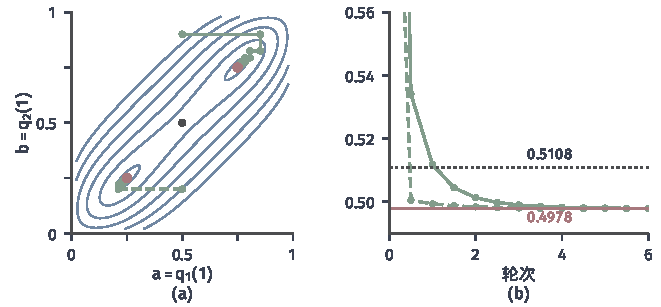
\includegraphics[width=112mm]{figures/07-probability/07-distribution-optimization/matplotlib/dapx-cavi-table/figure.pdf}
 \caption{概率表~\eqref{eq:dapx-table}上的逐因子更新。(a)乘积候选的目标值$D_{\mathrm{KL}}(q_1\otimes q_2\Vert\Pi)$关于$(a,b)$的等高线（蓝），红点是两个最小点$(\tfrac14,\tfrac14)$与$(\tfrac34,\tfrac34)$，深灰点是鞍点$(\tfrac12,\tfrac12)$；绿色实线是从$b^{(0)}=0.9$出发的路径，绿色虚线从$b^{(0)}=0.2$出发，每段折线对应一次因子更新。(b)每次因子更新后的目标值，横轴以轮计；红线是最小值$0.4978$，深灰点线是鞍点的值$0.5108$。}
 \label{fig:dapx-cavi-table}
\end{BookInlineFigure}

计算量取决于$g_j$是否容易求。若$\ln\widetilde{\pi}$是许多只涉及少数变量的项之和，例如前面的成对作用模型，那么$g_j(x_j)$只需要与$x_j$同在一项里的那些变量的因子：对二值变量，它等于$x_j$乘以$h_j+\sum_{k\neq j}J_{j,k}q_k(1)$再加常数（这里约定$J_{j,k}=J_{k,j}$），一次更新的代价与$x_j$参与的项数成正比，一轮的代价与项的总数成正比，而不是$2^{m}$。若$\ln\widetilde{\pi}$把许多变量缠在一个不可分的式子里，$g_j$本身就是一个高维期望，坐标更新也就失去了计算上的好处。

\section{参数的梯度更新}
\label{sec:dapx-gradient}

逐因子更新依赖一个前提：每个因子可以是任意分布，于是“取指数再归一化”的结果总在候选集合里。若要求因子属于某个参数族，比如规定每个因子都是高斯分布，而目标不是高斯分布，式~\eqref{eq:dapx-cavi-update}给出的$\exp(g_j)$一般不再是高斯密度，更新会跳出候选集合。又比如章首的四次方目标只有一个变量，没有可以拆分的因子。这时候选集合是一个有限维参数族，逼近问题就成了参数的优化问题。

\paragraph{参数优化问题}
设候选集合为$\{Q_{\bm{\theta}}:\bm{\theta}\in\Theta\}$，$\Theta\subset\mathbb{R}^{d}$是开集，密度$q_{\bm{\theta}}$对$\bm{\theta}$可微。按候选加权的方向，由式~\eqref{eq:dapx-J}，要最小化
\begin{equation}
 J(\bm{\theta})=\mathbb{E}_{Q_{\bm{\theta}}}\bigl[\ln q_{\bm{\theta}}(X)-\ln\widetilde{\pi}(X)\bigr] .
 \label{eq:dapx-J-theta}
\end{equation}
按目标加权的方向，在式~\eqref{eq:dapx-forward-split}成立的范围内，要最小化$-\mathbb{E}_{\Pi}[\ln q_{\bm{\theta}}(X)]$。只要目标函数可微，就可以用\BookChapterRef{chap:first-order-methods}{卷五第6章“一阶方法”}的梯度下降，
\begin{equation}
 \bm{\theta}^{(t+1)}=\bm{\theta}^{(t)}-\eta\,\nabla J\bigl(\bm{\theta}^{(t)}\bigr) ,
 \label{eq:dapx-gd}
\end{equation}
其中$\eta>0$是步长。参数还可以与乘积结构结合：每个因子取一个参数族，对所有因子的参数一起做梯度更新，或者在没有闭式解的那些因子上用梯度步代替式~\eqref{eq:dapx-cavi-update}。

两个方向的梯度对计算的要求不同。按目标加权时，在求导与期望可以交换的条件下，
\[
 \nabla_{\bm{\theta}}\bigl(-\mathbb{E}_{\Pi}[\ln q_{\bm{\theta}}(X)]\bigr)=-\mathbb{E}_{\Pi}\bigl[\nabla_{\bm{\theta}}\ln q_{\bm{\theta}}(X)\bigr] ,
\]
期望仍按目标计算；对指数族它就是$\nabla A(\bm{\theta})-\mathbb{E}_{\Pi}[\bm{T}]$，零点正是定理~\ref{thm:dapx-moment-matching}的矩匹配。按候选加权时，被积函数和求期望的分布都依赖$\bm{\theta}$，求导要同时处理两处。本节的例子里期望有闭式，可以直接求导；没有闭式时，要用样本构造梯度的随机估计，什么时候能交换求导与期望、怎样构造方差小的估计，是第~\ref{chap:expectation-gradient-estimation}章的内容，有了随机梯度后的迭代方法见\BookChapterRef{chap:stochastic-gradient-methods}{卷五第13章“随机梯度方法”}。

\paragraph{按目标加权：指数族上的凸问题}
候选是指数族时，按目标加权的目标函数在自然参数下是凸的。在式~\eqref{eq:dapx-forward-split}成立的范围内，与$\bm{\theta}$有关的部分是
\[
 -\mathbb{E}_{\Pi}[\ln q_{\bm{\theta}}(X)]=A(\bm{\theta})-\langle\bm{\theta},\mathbb{E}_{\Pi}[\bm{T}]\rangle-\mathbb{E}_{\Pi}[\ln h(X)] .
\]
第~\ref{chap:distribution-families}章证明了$A$的Hessian是$\bm{T}$的协方差矩阵，半正定，所以$A$是凸函数，再减去一个线性函数仍是凸的。凸函数的驻点就是全局最小点，梯度下降不会停在别处。

用三状态例子走几步。$Q_t$的自然参数$\theta$满足$t=\mathrm{e}^{\theta}/(1+2\mathrm{e}^{\theta})$，对数配分函数$A(\theta)=\ln(1+2\mathrm{e}^{\theta})$，$A'(\theta)=2t$，所以梯度就是矩的差：
\[
 \frac{\mathrm{d}}{\mathrm{d}\theta}D_{\mathrm{KL}}(\Pi\Vert Q_t)=2t-0.7 .
\]
取步长$\eta=2$，从$\theta^{(0)}=0$即$t=\tfrac13$出发。第一步的梯度是$\tfrac23-0.7=-0.0333$，于是
\[
 \theta^{(1)}=0+2\cdot0.0333=0.0667,\qquad t^{(1)}=0.3407 .
\]
第二步梯度为$-0.0187$，得到
\[
 \theta^{(2)}=0.104,\qquad t^{(2)}=0.3447 .
\]
在最优点附近，二阶导数$A''(\theta^{*})$等于$2t_{\mathrm{f}}(1-2t_{\mathrm{f}})=0.21$，梯度每步约乘以
\[
 1-\eta A''(\theta^{*})=1-2\cdot0.21=0.58 .
\]
第$7$步$t=0.3497$，趋于$t_{\mathrm{f}}=0.35$，对应$\theta^{*}=\ln(0.35/0.3)\approx0.154$。

按候选加权的目标函数没有这样的结构。它依赖$\bm{\theta}$的方式既通过$\ln q_{\bm{\theta}}$，也通过求期望的分布本身，在自然参数下一般不是凸的：第~\ref{sec:dapx-direction-compare}节双峰目标上的两个局部最小点就是例子。所以按候选加权时，梯度下降的结果要结合初值来解释。

\paragraph{参数化保持合法}
梯度步是在$\mathbb{R}^{d}$里走一步，走完后的参数必须仍然对应一个合法的分布。对四次方目标取候选$\mathcal{N}(m,s^{2})$，若直接以$(m,s)$为参数，由式~\eqref{eq:dapx-quartic-J}，
\[
 \frac{\partial J}{\partial s}=-\frac1s+3m^{2}s+3s^{3} .
\]
在$m=0$、$s=1.5$处它等于$-0.667+10.125=9.458$，取步长$\eta=0.2$，一步后$s=1.5-1.892<0$，不再是标准差。

改用$\omega=\ln s$作参数，$s=\mathrm{e}^{\omega}$对任何实数$\omega$都是正的，约束自动满足。由链式法则，
\[
 \frac{\partial J}{\partial\omega}=s\,\frac{\partial J}{\partial s}=1.5\cdot9.458=14.19 .
\]
同样的步长下，一步后
\[
 \omega=\ln1.5-0.2\cdot14.19=-2.43,\qquad s=\mathrm{e}^{-2.43}\approx0.088 .
\]
这个$s$合法，却走得太远，说明步长仍要另行选择；重新参数化只解决合法性。同样的办法用于其他约束：概率向量写成$p_k=\mathrm{e}^{u_k}/\sum_l\mathrm{e}^{u_l}$；协方差矩阵写成$\bm{L}\bm{L}^{\top}$，$\bm{L}$是对角元取指数的下三角矩阵，于是总是对称正定。

\paragraph{四次方目标的梯度下降}
以$(m,\omega)$为参数，把$s=\mathrm{e}^{\omega}$代入式~\eqref{eq:dapx-quartic-J}：
\[
 J(m,\omega)=-\omega-C+\tfrac14\bigl(m^{4}+6m^{2}\mathrm{e}^{2\omega}+3\mathrm{e}^{4\omega}\bigr) .
\]
分别求偏导，得到
\begin{equation}
 \frac{\partial J}{\partial m}=m^{3}+3ms^{2},\qquad \frac{\partial J}{\partial\omega}=-1+3m^{2}s^{2}+3s^{4} .
 \label{eq:dapx-quartic-grad}
\end{equation}
梯度为零要求$m(m^{2}+3s^{2})=0$，即$m=0$，再由第二式得$s^{4}=\tfrac13$，与第~\ref{sec:dapx-reverse-kl}节的结果一致。

取$\eta=0.1$，从$(m,\omega)=(1,0)$即$\mathcal{N}(1,1)$出发。第一步的梯度由式~\eqref{eq:dapx-quartic-grad}算出：
\[
 \frac{\partial J}{\partial m}=1+3=4,\qquad \frac{\partial J}{\partial\omega}=-1+3+3=5 .
\]
由式~\eqref{eq:dapx-gd}，
\[
 m^{(1)}=1-0.4=0.6,\qquad \omega^{(1)}=0-0.5=-0.5,\qquad s^{(1)}=\mathrm{e}^{-0.5}\approx0.6065 .
\]
第二步$s^{2}\approx0.3679$，$s^{4}\approx0.1353$，梯度为
\[
 \begin{aligned}
 \frac{\partial J}{\partial m}&=0.216+3\cdot0.6\cdot0.3679=0.8782,\\
 \frac{\partial J}{\partial\omega}&=-1+3\cdot0.36\cdot0.3679+3\cdot0.1353=-0.1967 ,
 \end{aligned}
\]
于是$m^{(2)}=0.5122$，$\omega^{(2)}=-0.4803$。

用$D_{\mathrm{KL}}=J+\ln Z$记录离目标的远近，前几步依次为$2.022$、$0.355$、$0.280$；第$10$步为$0.0654$，第$20$步为$0.0476$，第$40$步与族内最小值$0.0472$相同到四位小数。图~\ref{fig:dapx-gradient-path}(a)中，第一步把$\omega$拉低了很多，此后路径沿着一条弯曲的谷慢慢移向最优点。

\begin{BookInlineFigure}
 \centering
 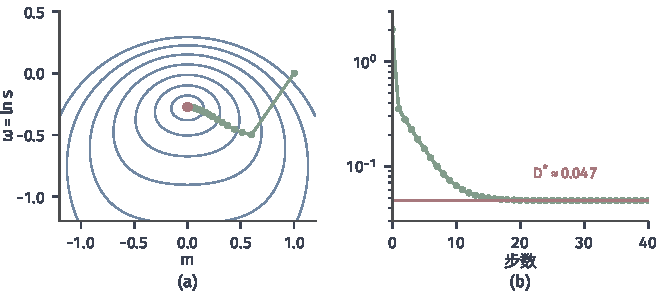
\includegraphics[width=112mm]{figures/07-probability/07-distribution-optimization/matplotlib/dapx-gradient-path/figure.pdf}
 \caption{四次方目标上高斯候选的梯度下降，参数$(m,\omega)$，$\omega=\ln s$，步长$0.1$。(a)$J(m,\omega)$的等高线（蓝）与$40$步的路径（绿），起点$(1,0)$，红点是最优解$(0,-\tfrac14\ln3)$。(b)各步的$D_{\mathrm{KL}}(Q^{(t)}\Vert\Pi)$（绿，对数纵轴），红线是族内最小值$0.0472$。}
 \label{fig:dapx-gradient-path}
\end{BookInlineFigure}

后期的收敛主要受$m$拖累。在最优点附近$s^{2}\approx3^{-1/2}$，$\partial J/\partial m\approx3s^{2}m\approx1.73\,m$，每步$m$乘以$1-0.173=0.827$，要把$m$从$0.1$降到$10^{-4}$约需$36$步。$\omega$方向的曲率不同，收敛快得多。各方向曲率不同时，同一个步长对某些方向太小、对另一些方向又可能太大，这是梯度下降在病态问题上的典型表现。在分布逼近中还有一层含义：参数空间里同样长的一步，在不同参数、不同位置引起的分布变化可能相差很大，$s$很小时改变$m$一点点，分布就几乎不再重叠。用分布本身的变化来度量步长、据此调整更新方向，是第~\ref{chap:information-geometry}章的内容。

\section{逼近误差的评价}
\label{sec:dapx-error}

算法停下来以后，手里有一个候选$\widehat{Q}$和一个算出的目标值。这个近似有多好？要回答这个问题，先要把误差的来源分开，再按后续任务选择检验的量。只看一个KL数值，既分不清误差从哪里来，也不知道它对任务意味着什么。

\paragraph{三个来源}
固定一个逼近目标，记为$\mathcal{L}(Q)$，例如$D_{\mathrm{KL}}(Q\Vert\Pi)$。设族内最优解$Q^{\dagger}\in\argmin_{Q\in\mathcal{Q}}\mathcal{L}(Q)$存在，算法输出$\widehat{Q}$，报告的目标值是$\widehat{\mathcal{L}}$。三者之间有恒等式
\begin{equation}
 \widehat{\mathcal{L}}=\underbrace{\mathcal{L}(Q^{\dagger})}_{\text{表达限制}}+\underbrace{\mathcal{L}(\widehat{Q})-\mathcal{L}(Q^{\dagger})}_{\text{优化差距}}+\underbrace{\widehat{\mathcal{L}}-\mathcal{L}(\widehat{Q})}_{\text{计算误差}} .
 \label{eq:dapx-error-parts}
\end{equation}
第一项只由目标和候选集合决定，与算法无关：候选集合里最好的分布离目标也有这么远。第二项非负，衡量算法离族内最优还差多少，它可能来自迭代步数不够，也可能来自停在了局部最优。第三项来自期望的数值计算，用样本平均估计期望时它是随机的，可正可负。图~\ref{fig:dapx-error-parts}示意了前两项。

\begin{BookInlineFigure}
 \centering
 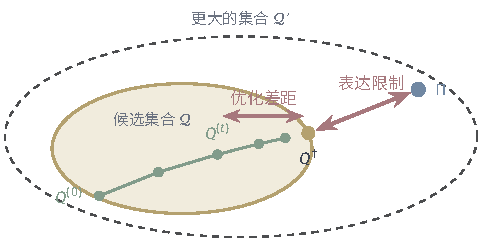
\includegraphics[width=82mm]{figures/07-probability/07-distribution-optimization/tikz/dapx-error-parts/figure.pdf}
 \caption{误差来源示意（不按比例，KL也不是几何距离）。黄色区域是候选集合$\mathcal{Q}$，蓝点是目标$\Pi$，黄点$Q^{\dagger}$是族内最优解；绿点是算法的迭代。$\Pi$到$Q^{\dagger}$的红色箭头是表达限制，迭代到$Q^{\dagger}$的红色箭头是优化差距。虚线是包含$\mathcal{Q}$的更大候选集合$\mathcal{Q}'$，它的表达限制不会更大。}
 \label{fig:dapx-error-parts}
\end{BookInlineFigure}

用四次方目标把三项都算出来。表达限制是高斯族内的最小KL，$0.0472$。第~\ref{sec:dapx-gradient}节的梯度下降做$10$步时KL为$0.0654$，优化差距是$0.0182$；做$40$步时差距已小于$10^{-4}$。计算误差来自对$J$的估计：若不用闭式~\eqref{eq:dapx-quartic-J}，而是从$Q$抽$n$个样本，用
\[
 \widehat{J}_n=\frac1n\sum_{i=1}^{n}\bigl(\ln q(X_i)-\ln\widetilde{\pi}(X_i)\bigr),\qquad X_i\sim Q\text{独立},
\]
估计$J(Q)$，它的标准差是$\sigma/\sqrt{n}$，$\sigma$是被积函数在$Q$下的标准差。在$Q^{*}$处模拟得$\sigma\approx0.409$。

$n=100$时估计的均方根误差约为$0.043$（$400$次重复，种子$727$），比第$10$步的优化差距$0.018$还大。也就是说，用$100$个样本估计目标值时，看不出第$10$步与最优解的差别；要分辨$0.018$这样的差距，需要把标准差压到它的几分之一，$n$要到几千。图~\ref{fig:dapx-mc-error}显示，误差按$n^{-1/2}$缩小，与$\sigma/\sqrt{n}$吻合。积分误差的一般理论与缩小方差的办法分别在第~\ref{chap:monte-carlo-integration-error}章和第~\ref{chap:variance-reduction}章展开。

\begin{BookInlineFigure}
 \centering
 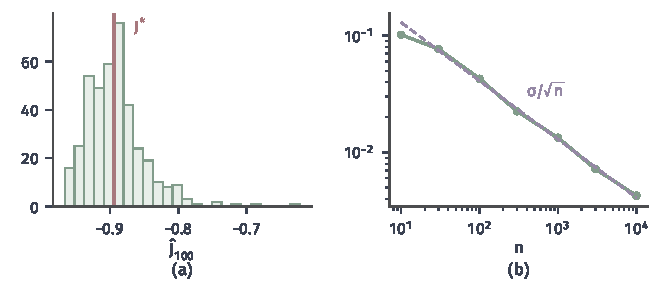
\includegraphics[width=112mm]{figures/07-probability/07-distribution-optimization/matplotlib/dapx-mc-error/figure.pdf}
 \caption{目标值的计算误差。候选为四次方目标的最优高斯$Q^{*}$，$J^{*}\approx-0.8943$。(a)$400$次独立重复中$n=100$的估计$\widehat{J}_{100}$（浅绿直方图）与真值（红线），标准差约$0.043$。(b)均方根误差随$n$的变化（绿，双对数坐标）与$\sigma/\sqrt{n}$（紫色虚线），$\sigma\approx0.409$。随机数种子为$727$。}
 \label{fig:dapx-mc-error}
\end{BookInlineFigure}

式~\eqref{eq:dapx-error-parts}还提醒一件事：当目标只有未归一化形式时，算出的是$J$而不是KL，第一项“表达限制”的大小未知，只知道$-J$是$\ln Z$的下界。比较几个候选或几个候选集合时，$J$的差就是KL的差，足以判断谁更好；要说“近似已经足够好”，则需要别的检验。

\paragraph{按任务检验}
后续任务若要用近似分布计算某些量，就应当直接检验这些量。对四次方目标，两个方向的最优高斯分别是$Q_{\mathrm{r}}=\mathcal{N}(0,0.5774)$与$Q_{\mathrm{f}}=\mathcal{N}(0,0.6760)$。比较二阶矩与四阶矩：
\[
 \begin{array}{lccc}
  & \Pi & Q_{\mathrm{r}} & Q_{\mathrm{f}}\\
 \mathbb{E}[X^{2}] & 0.676 & 0.577 & 0.676\\
 \mathbb{E}[X^{4}] & 1 & 1 & 1.371
 \end{array}
\]
目标的四阶矩由$\Gamma(5/4)=\tfrac14\Gamma(1/4)$得到：
\[
 \mathbb{E}_{\Pi}[X^{4}]=\frac{4\,\Gamma(5/4)}{\Gamma(1/4)}=1 .
\]
按目标加权的解匹配了二阶矩，这是矩匹配的直接结果，四阶矩却高估了$37\%$。按候选加权的解低估了二阶矩约$15\%$，四阶矩却恰好正确。图~\ref{fig:dapx-moment-compare}画出三个密度：目标的顶部更平、两侧下降更陡，两个高斯都无法同时匹配这两个特征。

后一个现象有原因。在候选$\mathcal{N}(0,s^{2})$中，把$X$写成$sY$，$J(s)=-\ln s-C-\mathbb{E}[\ln\widetilde{\pi}(sY)]$。对$s$求导并令其为零，再乘以$s$，得到最优尺度满足
\[
 \mathbb{E}_{Q_{\mathrm{r}}}\bigl[X\,(\ln\widetilde{\pi})'(X)\bigr]=-1 .
\]
另一方面，若$\pi$可微且$x\pi(x)\to0$（$\lvert x\rvert\to\infty$），分部积分给出
\[
 \mathbb{E}_{\Pi}\bigl[X\,(\ln\pi)'(X)\bigr]=\int x\pi'(x)\,\mathrm{d}x=-\int\pi(x)\,\mathrm{d}x=-1 .
\]
两式的左边是同一个函数$x(\ln\widetilde{\pi})'(x)$在两个分布下的期望。四次方目标中这个函数是$-x^{4}$，所以两个分布的四阶矩相同。可见，每个方向只“保留”与自己的驻点方程相关的那些平均，其余的量要单独检验。

\begin{BookInlineFigure}
 \centering
 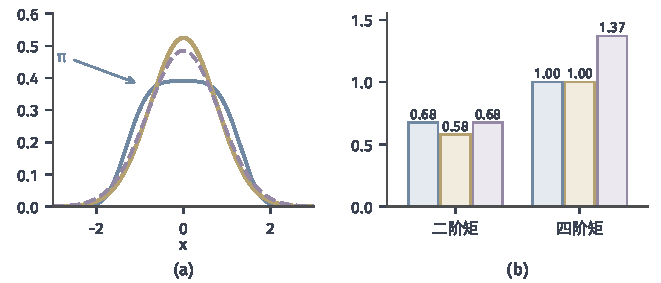
\includegraphics[width=112mm]{figures/07-probability/07-distribution-optimization/matplotlib/dapx-moment-compare/figure.pdf}
 \caption{四次方目标的两个高斯近似。(a)目标密度（蓝），按候选加权的最优解$\mathcal{N}(0,0.577)$（黄），按目标加权的最优解$\mathcal{N}(0,0.676)$（紫色虚线）。(b)三个分布的二阶矩与四阶矩，颜色同(a)。}
 \label{fig:dapx-moment-compare}
\end{BookInlineFigure}

关心事件概率时，可以用第~\ref{chap:distribution-comparison}章的Pinsker不等式$d_{\mathrm{TV}}\leq\sqrt{D_{\mathrm{KL}}/2}$。总变差是对称的，两个方向的KL都可以代入。对$Q_{\mathrm{r}}$，$D_{\mathrm{KL}}(Q_{\mathrm{r}}\Vert\Pi)\approx0.0472$给出$d_{\mathrm{TV}}\leq0.154$，数值积分得到的真值是$0.115$。对$Q_{\mathrm{f}}$，$D_{\mathrm{KL}}(\Pi\Vert Q_{\mathrm{f}})\approx0.0317$给出$d_{\mathrm{TV}}\leq0.126$，真值是$0.094$。这个上界对所有事件同时成立，但对具体的事件往往很松：$\mathbb{P}(\lvert X\rvert>1.5)$在目标下是$0.0462$，在$Q_{\mathrm{r}}$下是$0.0484$，在$Q_{\mathrm{f}}$下是$0.0681$，按候选加权的近似在这个尾概率上反而更好。

\paragraph{无界的检验函数}
若要检验的是无界函数的期望，比如矩，总变差和KL本身都不够，必须有尾部条件。第~\ref{chap:distribution-comparison}章证明了：KL要控制$g$的期望差，需要$g$在参考分布下有指数矩。反例很简单。目标为标准Cauchy分布、候选为高斯分布时，第~\ref{sec:dapx-target-candidates}节已经看到$D_{\mathrm{KL}}(Q\Vert\Pi)$有限，可是$\mathbb{E}_{\Pi}[X^{2}]=+\infty$，而每个高斯候选的二阶矩都有限。无论KL被优化到多小，用这个近似计算二阶矩都没有意义。所以，按任务检验时要先确认待求的量在目标下存在，再确认所用的比较量能控制它。

\paragraph{扩大候选集合}
若$\mathcal{Q}\subset\mathcal{Q}'$，则
\[
 \inf_{Q\in\mathcal{Q}'}\mathcal{L}(Q)\leq\inf_{Q\in\mathcal{Q}}\mathcal{L}(Q) ,
\]
因为在更大的集合里取下确界，可选的更多。这只说明式~\eqref{eq:dapx-error-parts}的第一项不会变大，并不说明实际算出的结果会变好：更大的候选集合往往带来更难的优化，第二项可能变大。

看式~\eqref{eq:dapx-bimodal}的双峰目标，目标值取$D_{\mathrm{KL}}(Q\Vert\Pi)$。单个高斯族内的最小值约为$0.356$，在左峰。两成分高斯混合族（权重、均值、方差都可变）包含目标本身，下确界为$0$。设对混合族做梯度下降，两个成分的权重都初始化为$\tfrac12$，均值和方差也取相同的值，放在右峰附近。交换两个成分不改变混合分布，所以目标值关于两组成分参数对称；在两组参数相同的点上，目标值对两组参数的偏导数也相同，每一步更新都保持两个成分相同，权重也一直是$\tfrac12$。这样的混合就是单个高斯，迭代实际上是在单个高斯族里进行，会停在右峰的局部最小点，值约为$1.202$。图~\ref{fig:dapx-larger-family}对比了这几个数。

\begin{BookInlineFigure}
 \centering
 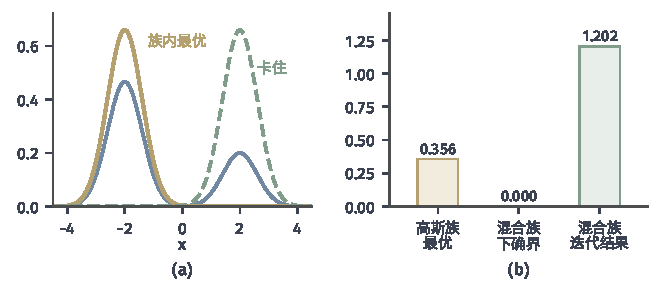
\includegraphics[width=112mm]{figures/07-probability/07-distribution-optimization/matplotlib/dapx-larger-family/figure.pdf}
 \caption{扩大候选集合不保证结果变好。(a)双峰目标（蓝）、单个高斯族内按候选加权的最优解$\mathcal{N}(-2,0.6^{2})$（黄），以及两成分完全相同地初始化在右峰附近的混合族迭代的结果（绿色虚线），它停在右峰的单个高斯上。(b)$D_{\mathrm{KL}}(Q\Vert\Pi)$：高斯族最优$0.356$，混合族下确界$0$，混合族迭代结果$1.202$。}
 \label{fig:dapx-larger-family}
\end{BookInlineFigure}

这个例子是刻意构造的，但它揭示的机制普遍存在：候选集合越大，目标函数的局部最优和对称结构往往越多。比较两个候选集合时，应当比较实际算出的结果，并报告初值与迭代设置；“族更大所以更准”只对下确界成立。

\section{本章小结}
\label{sec:dapx-summary}

章首的问题是：给定一个只能逐点计算未归一化密度的分布，怎样找一个容易计算的分布代替它。本章把这个问题拆成四个选择，每个选择都有自己的依据和代价。表~\ref{tab:dapx-summary}把它们并列。

\begin{BookInlineTable}
 \centering
 \caption{逼近问题中的四个选择。}
 \label{tab:dapx-summary}
 \begin{tabular}{lll}
  \toprule
  选择 & 选项 & 依据与代价\\
  \midrule
  候选集合 & 乘积结构 & 删去组间依赖，因子形状不限\\
   & 有限维参数族 & 限制形状，参数须保持合法\\
  KL方向 & $D_{\mathrm{KL}}(Q\Vert\Pi)$ & 需$Q\ll\Pi$；只需$\widetilde{\pi}$与$Q$下期望\\
   & $D_{\mathrm{KL}}(\Pi\Vert Q)$ & 需$\Pi\ll Q$；需$\Pi$下期望或样本\\
  求解 & 逐因子更新 & 子问题有闭式解，目标值单调下降\\
   & 参数梯度 & 适用于参数族，需梯度与步长\\
  评价 & 误差分解 & 表达限制、优化差距、计算误差\\
   & 按任务检验 & 矩、事件概率；无界函数要尾部条件\\
  \bottomrule
 \end{tabular}
\end{BookInlineTable}

候选集合决定了能保留什么。乘积候选无论怎样选择，都不能表示组间的依赖：概率表上两个变量常常相等的事实、相关高斯中的协方差都会消失。有限维参数族限制的是形状，单个高斯不能有两个峰，也不能像四次方目标那样有比高斯更轻的尾。这些损失在逼近开始之前就已确定，即式~\eqref{eq:dapx-error-parts}中的表达限制。

KL方向决定了在这些损失之间怎样取舍。按候选加权的方向惩罚候选在目标稀少处放置的质量，只要求逐点计算$\widetilde{\pi}$，因此在目标难算时最常用；它的最优解在三状态例子里给中间状态多分了概率，在相关高斯中把方差压到条件方差$1-\rho^{2}$，在双峰目标上贴住一个峰。按目标加权的方向惩罚候选对目标的覆盖不足，对指数族候选就是矩匹配，却需要目标下的期望。两个方向选出的分布一般不同，“择峰”与“覆盖”只是倾向，具体结论要按例子计算。

求解方法由候选集合的类型决定。乘积候选且因子不受限制时，每个因子的最优更新是对其余因子平均目标的对数密度，再取指数并归一化；每次更新不增加目标值，但只保证目标值收敛，可能停在鞍点或局部最优。参数族候选则用梯度下降，重新参数化保证每一步仍是合法分布，期望没有闭式时需要随机梯度。

评价时要分清误差的来源，并直接检验任务关心的量。四次方目标上，表达限制是$0.0472$，$10$步梯度下降后的优化差距是$0.018$，而用$100$个样本估计目标值的误差约为$0.043$，足以掩盖优化差距。两个方向的最优高斯分别保留了四阶矩和二阶矩，各自在另一个矩上有明显误差。扩大候选集合只降低表达限制的下确界，实际结果还取决于优化能否找到好的解。

本章假定目标分布已经给定。在统计推断中，后验分布常常正是这样一个只知道未归一化密度的目标，本章的方法可以直接用于计算它的近似；后验分布怎样由先验与数据建立、近似结果在统计上意味着什么，见\BookChapterRef{chap:parametric-statistical-inference}{卷八第1章“参数化统计推断”}。参数空间中同样长的一步引起的分布变化不同，怎样按分布的变化来度量并选择更新方向，由第~\ref{chap:information-geometry}章研究。不用近似分布、直接从目标抽样来计算期望的方法，以及这些期望估计的误差与方差，由第~\ref{chap:sample-generation}章至第~\ref{chap:expectation-gradient-estimation}章研究。


\chapter{信息几何}
\label{chap:information-geometry}

在高斯族$\mathcal{N}(\mu,\sigma^{2})$中把均值增加$0.5$。若$\sigma=0.5$，新旧两个密度的峰几乎错开，两者的KL散度等于$0.5$；若$\sigma=2$，两条钟形曲线几乎重合，KL散度只有$1/32$。参数走了同样远，分布却变化了相差十六倍的量，如图~\ref{fig:igeo-same-shift}。

\begin{BookInlineFigure}
  \centering
  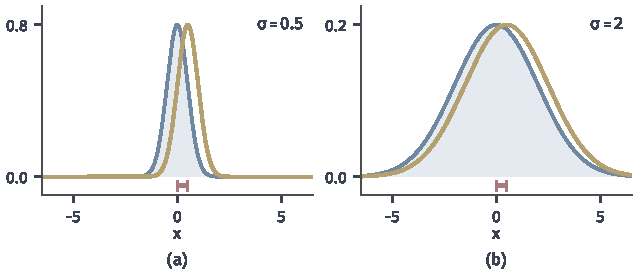
\includegraphics[width=108mm]{figures/07-probability/07-distribution-optimization/matplotlib/igeo-same-shift/figure.pdf}
  \caption{同样的均值位移$0.5$（红色短线）在两个尺度下引起的变化。蓝线并加浅蓝底是$\mathcal{N}(0,\sigma^{2})$，黄线是$\mathcal{N}(0.5,\sigma^{2})$。(a)$\sigma=0.5$，两者的KL散度为$0.5$；(b)$\sigma=2$，KL散度为$1/32$。}
  \label{fig:igeo-same-shift}
\end{BookInlineFigure}

方差方向也一样。把方差从$0.1$增加到$0.2$，KL散度约为$0.097$；把方差从$10$增加到$10.1$，KL散度只有约$2.5\times10^{-5}$。若改用对数方差$\tau=\ln\sigma^{2}$作参数，情况又不同：$\tau$增加同一个量，KL散度与起点的方差无关。参数的欧氏长度不是分布变化的尺度，而且换一套坐标，数值关系就跟着改变。

第~\ref{chap:distribution-approximation}章把族内逼近写成有限维参数的优化。普通梯度下降默认参数的每个方向“一样贵”，上面的例子说明这一默认并不成立：在$\sigma$很小的地方，均值稍动一点分布就大变；在方差很大的地方，方差改动很多分布也几乎不变。本章研究三个问题：参数的微小位移怎样引起分布变化，这种变化的大小用什么来度量；换一套参数坐标时，这个度量中什么改变、什么不变；怎样用它选择参数的更新方向。把分布族当作带有这种局部尺度的几何对象来研究，这套方法称为\term{信息几何}（information geometry）。

第一节规定可以逐点求导、并能与积分交换的分布族，定义得分函数与Fisher信息。第二节由邻近分布之间KL散度的二阶展开说明Fisher信息正是局部尺度，再检查它在坐标变换下的规律。第三节在指数族中核验这些结构，对数配分函数的导数同时给出Fisher信息与两套坐标的转换。第四节在相同的局部分布变化下寻找目标下降最多的方向，得到自然梯度，并说明它与坐标的关系。第五节讨论怎样实际计算这个方向和步长。

本章用到第~\ref{chap:distribution-families}章的指数族与均值映射，第~\ref{chap:distribution-comparison}章的KL散度及两个高斯分布之间的KL公式，以及第~\ref{chap:distribution-approximation}章的逼近目标。全章贯穿高斯族$\mathcal{N}(\mu,\sigma^{2})$在几套坐标下的计算。

\section{正则分布族}
\label{sec:igeo-regular}

要谈“参数动一点，分布变多少”，先得让“动一点”在每个位置上都有意义。固定可测空间$(\mathcal{X},\mathcal{F})$上的一个$\sigma$有限参考测度$\nu$，参数$\bm{\theta}$取值于$\mathbb{R}^{k}$的子集$\Theta$，每个$\bm{\theta}$对应一个相对$\nu$的密度$p_{\bm{\theta}}$与概率分布$P_{\bm{\theta}}$。对固定的$x$，$p_{\bm{\theta}}(x)$是$\bm{\theta}$的普通函数，可以对它求偏导数；分布的变化却还要把这些逐点的变化积分起来。于是需要两类条件：逐点可微，以及求导与积分可以交换。

\begin{definition}[正则分布族]
\label{def:igeo-regular-family}
称$\{p_{\bm{\theta}}:\bm{\theta}\in\Theta\}$为\term{正则分布族}（regular family），若下列条件成立：
\begin{enumerate}
  \item $\Theta$是$\mathbb{R}^{k}$中的非空开集；
  \item 支撑$S=\{x:p_{\bm{\theta}}(x)>0\}$不依赖$\bm{\theta}$；
  \item 对每个$x\in S$，$\bm{\theta}\mapsto p_{\bm{\theta}}(x)$在$\Theta$上连续可微；
  \item 对每个$\bm{\theta}\in\Theta$，$\int_{S}\lVert\nabla_{\bm{\theta}}p_{\bm{\theta}}\rVert_2\,\mathrm{d}\nu<\infty$，并且
  \begin{equation}
    \int_{S}\nabla_{\bm{\theta}}p_{\bm{\theta}}(x)\,\nu(\mathrm{d}x)=\nabla_{\bm{\theta}}\int_{S}p_{\bm{\theta}}(x)\,\nu(\mathrm{d}x)=\bm{0}.
    \label{eq:igeo-exchange}
  \end{equation}
\end{enumerate}
\end{definition}

四个条件各管一件事。开集保证从$\bm{\theta}$出发可以朝任何方向走一小步而不离开参数范围。共同支撑保证$\ln p_{\bm{\theta}}(x)$对所有参数都在同一个集合$S$上有定义，比较两个邻近分布时不会出现一边有质量、另一边为零的位置。逐点可微给出每个位置上密度的变化率。最后一条说：先对每个位置求变化率再积分，等于先积分再求导；而积分恒为$1$，所以结果为零向量。

式~\eqref{eq:igeo-exchange}的交换通常用控制收敛来保证。设$\bm{\theta}$有一个凸邻域$U$和$\nu$可积的函数$M$，使对所有$\bm{\theta}'\in U$与$x\in S$有
\[
  \lVert\nabla_{\bm{\theta}}p_{\bm{\theta}'}(x)\rVert_2\leq M(x).
\]
由中值定理，沿任一坐标方向的差商$\bigl(p_{\bm{\theta}+h\bm{e}_j}(x)-p_{\bm{\theta}}(x)\bigr)/h$的绝对值不超过$M(x)$，而当$h\to0$时它逐点趋于偏导数；控制收敛定理于是允许在积分号下取这个极限，可参考\BookChapterRef{chap:integration}{卷四第6章“积分”}。高斯族就满足这一条件：参数限制在紧邻域内时，密度的偏导数不超过一个多项式乘以$\mathrm{e}^{-cx^{2}}$，后者可积。

定义里没有要求后面将定义的Fisher信息正定。正则性只保证一阶的计算可以进行；参数是否冗余、局部变化是否退化，是另外需要检查的事情。

\subsection{得分函数}
\label{sec:igeo-score}

参数从$\bm{\theta}$变到$\bm{\theta}+\bm{\delta}$时，位置$x$处的密度从$p_{\bm{\theta}}(x)$变到$p_{\bm{\theta}+\bm{\delta}}(x)$。比较两个分布时，要紧的往往不是密度差了多少，而是差了百分之几：KL散度、似然比都只依赖密度之比。一阶近似下，相对变化是
\[
  \frac{p_{\bm{\theta}+\bm{\delta}}(x)-p_{\bm{\theta}}(x)}{p_{\bm{\theta}}(x)}\approx\frac{\langle\nabla_{\bm{\theta}}p_{\bm{\theta}}(x),\bm{\delta}\rangle}{p_{\bm{\theta}}(x)}=\langle\nabla_{\bm{\theta}}\ln p_{\bm{\theta}}(x),\bm{\delta}\rangle .
\]
尾部某个位置的密度可能很小，绝对变化也很小，但相对变化可以很大；对数导数正好记录的是后者。

\begin{definition}[得分函数]
\label{def:igeo-score}
设分布族正则。对$x\in S$，称
\begin{equation}
  \bm{s}_{\bm{\theta}}(x)=\nabla_{\bm{\theta}}\ln p_{\bm{\theta}}(x)=\frac{\nabla_{\bm{\theta}}p_{\bm{\theta}}(x)}{p_{\bm{\theta}}(x)}
  \label{eq:igeo-score}
\end{equation}
为\term{得分函数}（score function）。它是$\mathbb{R}^{k}$值函数，第$j$个分量记录沿第$j$个参数方向，$x$处密度的相对变化率。
\end{definition}

把概率看成总量为$1$的质量，参数变化只是把质量在各位置之间重新分配，不能凭空增减。某些位置的质量相对增加，另一些位置就必须相对减少，按质量加权以后正负抵消。下面的引理把这一点写成公式。

\begin{lemma}[得分的期望为零]
\label{lem:igeo-score-mean}
设分布族正则，$X\sim P_{\bm{\theta}}$，则$\mathbb{E}_{\bm{\theta}}\lVert\bm{s}_{\bm{\theta}}(X)\rVert_2<\infty$，并且
\begin{equation}
  \mathbb{E}_{\bm{\theta}}[\bm{s}_{\bm{\theta}}(X)]=\bm{0}.
  \label{eq:igeo-score-mean}
\end{equation}
\end{lemma}

\begin{proof}
$P_{\bm{\theta}}$的质量全部在$S$上；在$S$上，由式~\eqref{eq:igeo-score}，得分乘以密度就是密度的梯度。于是
\[
  \mathbb{E}_{\bm{\theta}}\lVert\bm{s}_{\bm{\theta}}(X)\rVert_2=\int_{S}\frac{\lVert\nabla_{\bm{\theta}}p_{\bm{\theta}}\rVert_2}{p_{\bm{\theta}}}\,p_{\bm{\theta}}\,\mathrm{d}\nu=\int_{S}\lVert\nabla_{\bm{\theta}}p_{\bm{\theta}}\rVert_2\,\mathrm{d}\nu<\infty ,
\]
期望存在。同样地，
\[
  \mathbb{E}_{\bm{\theta}}[\bm{s}_{\bm{\theta}}(X)]=\int_{S}\nabla_{\bm{\theta}}p_{\bm{\theta}}\,\mathrm{d}\nu ,
\]
由式~\eqref{eq:igeo-exchange}，右端为零向量。
\end{proof}

\paragraph{高斯族的两个得分}
取$\nu$为Lebesgue测度，参数为$(\mu,\sigma)$，$\sigma>0$。对数密度是
\[
  \ln p_{\mu,\sigma}(x)=-\ln\sigma-\frac12\ln(2\pi)-\frac{(x-\mu)^{2}}{2\sigma^{2}} .
\]
记标准化的位置$z=(x-\mu)/\sigma$。分别对$\mu$与$\sigma$求偏导数，得到
\begin{equation}
  s_{\mu}(x)=\frac{x-\mu}{\sigma^{2}}=\frac{z}{\sigma},\qquad
  s_{\sigma}(x)=-\frac1\sigma+\frac{(x-\mu)^{2}}{\sigma^{3}}=\frac{z^{2}-1}{\sigma}.
  \label{eq:igeo-gauss-score}
\end{equation}
$Z=(X-\mu)/\sigma$服从$\mathcal{N}(0,1)$，$\mathbb{E}[Z]=0$，$\mathbb{E}[Z^{2}]=1$，所以两个得分的期望都是零，与引理~\ref{lem:igeo-score-mean}一致。

两个得分讲的是两种不同的重新分配。增大均值时，$s_{\mu}$在$x>\mu$处为正、在$x<\mu$处为负：右边的质量相对增加，左边相对减少，整体向右挪。增大$\sigma$时，$s_{\sigma}$在$\lvert z\rvert>1$处为正、在$\lvert z\rvert<1$处为负：中间的质量被搬到两边的尾部。图~\ref{fig:igeo-score-density}的下排画出$p\,s=\partial p/\partial\theta$，浅蓝与浅红两块面积相等，这正是式~\eqref{eq:igeo-score-mean}。

\begin{BookInlineFigure}
  \centering
  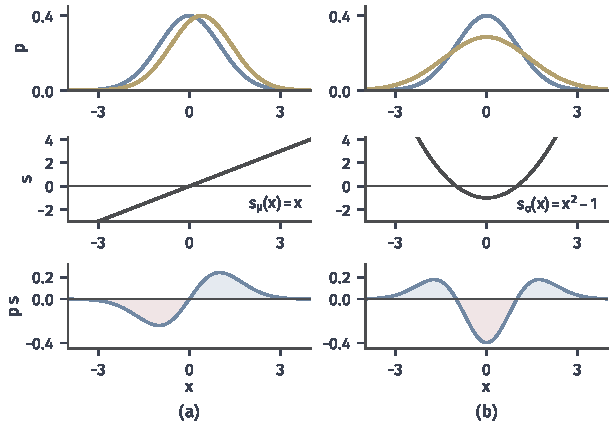
\includegraphics[width=104mm]{figures/07-probability/07-distribution-optimization/matplotlib/igeo-score-density/figure.pdf}
  \caption{$\mathcal{N}(0,1)$处的两个得分。(a)改变均值；(b)改变尺度$\sigma$。上排：蓝线为$\mathcal{N}(0,1)$，黄线为参数改变后的密度（(a)为$\mathcal{N}(0.4,1)$，(b)为$\mathcal{N}(0,1.4^{2})$）。中排：得分函数$s(x)$。下排：密度对参数的导数$p\,s$，浅蓝为质量相对增加的区域，浅红为相对减少的区域，两块面积相等，(a)中各约$0.399$，(b)中各约$0.483$。}
  \label{fig:igeo-score-density}
\end{BookInlineFigure}

\paragraph{支撑随参数移动}
共同支撑不能省。取$\operatorname{Unif}(0,\theta)$，$\theta>0$，在$(0,\theta)$上$p_{\theta}(x)=1/\theta$。对这些$x$，
\[
  \frac{\partial}{\partial\theta}\ln p_{\theta}(x)=-\frac1\theta ,
\]
它是常数，期望等于$-1/\theta\neq0$。引理~\ref{lem:igeo-score-mean}失效，原因是对积分上限也随$\theta$变化的积分求导会多出一项边界值：
\[
  \frac{\mathrm{d}}{\mathrm{d}\theta}\int_{0}^{\theta}\frac1\theta\,\mathrm{d}x=\underbrace{\frac1\theta}_{\text{边界项}}+\int_{0}^{\theta}\Bigl(-\frac1{\theta^{2}}\Bigr)\mathrm{d}x=\frac1\theta-\frac1\theta=0 .
\]
积分号内的部分正是得分的期望$-1/\theta$；边界项$1/\theta$是新出现在$\theta$右侧的质量，得分只定义在旧支撑上，看不到它。

图~\ref{fig:igeo-uniform-boundary}把这一点画了出来。$\theta$增大到$\theta+h$时，旧支撑内的密度整体下降，损失的质量$h/(\theta+h)$恰好出现在旧支撑外的$(\theta,\theta+h]$上。质量守恒的类比在这里仍然成立，只是新增的那部分落在得分看不到的地方。对这类模型，后面关于Fisher信息与局部KL的结论都不能直接套用：只要$h<0$，$P_{\theta}$在$(\theta+h,\theta)$上有质量而$P_{\theta+h}$没有，于是
\[
  D_{\mathrm{KL}}(P_{\theta}\Vert P_{\theta+h})=\infty .
\]

\begin{BookInlineFigure}
  \centering
  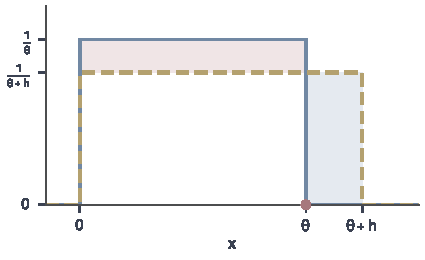
\includegraphics[width=72mm]{figures/07-probability/07-distribution-optimization/matplotlib/igeo-uniform-boundary/figure.pdf}
  \caption{支撑随参数移动的均匀分布，$\theta=1$，$h=0.25$。蓝线为$\operatorname{Unif}(0,\theta)$的密度，黄色虚线为$\operatorname{Unif}(0,\theta+h)$的密度。浅红区域是旧支撑内减少的质量$0.2$，浅蓝区域是旧支撑外新增的质量$0.2$；红点标出移动的端点。}
  \label{fig:igeo-uniform-boundary}
\end{BookInlineFigure}

\subsection{Fisher信息}
\label{sec:igeo-fisher}

得分是一个均值为零的随机向量。它的取值越分散，参数的小变化在各处造成的相对变化就越大，分布也就越容易与原来区分开。沿方向$\bm{u}\in\mathbb{R}^{k}$，密度的相对变化率是$\langle\bm{u},\bm{s}_{\bm{\theta}}(X)\rangle$，它的均方
\[
  \mathbb{E}_{\bm{\theta}}\bigl[\langle\bm{u},\bm{s}_{\bm{\theta}}(X)\rangle^{2}\bigr]=\bm{u}^{\top}\,\mathbb{E}_{\bm{\theta}}\bigl[\bm{s}_{\bm{\theta}}(X)\bm{s}_{\bm{\theta}}(X)^{\top}\bigr]\,\bm{u}
\]
是一个关于$\bm{u}$的二次型。中间的矩阵把所有方向的信息收在一起。

\begin{definition}[Fisher信息矩阵]
\label{def:igeo-fisher}
设分布族正则，且$\mathbb{E}_{\bm{\theta}}\lVert\bm{s}_{\bm{\theta}}(X)\rVert_2^{2}<\infty$。称$k\times k$矩阵
\begin{equation}
  \bm{G}(\bm{\theta})=\mathbb{E}_{\bm{\theta}}\bigl[\bm{s}_{\bm{\theta}}(X)\bm{s}_{\bm{\theta}}(X)^{\top}\bigr]
  \label{eq:igeo-fisher}
\end{equation}
为$\bm{\theta}$处的\term{Fisher信息矩阵}（Fisher information matrix），简称Fisher信息。
\end{definition}

由引理~\ref{lem:igeo-score-mean}，得分的均值为零，所以
\[
  \bm{G}(\bm{\theta})=\operatorname{Cov}_{\bm{\theta}}\bigl(\bm{s}_{\bm{\theta}}(X)\bigr),
\]
Fisher信息就是得分的协方差矩阵。这里用$\bm{G}$而不用常见的$I$，是为了与互信息$I(X;Y)$区分。

Fisher信息总是对称半正定的。对任意$\bm{u}$，
\[
  \bm{u}^{\top}\bm{G}(\bm{\theta})\bm{u}=\mathbb{E}_{\bm{\theta}}\bigl[\langle\bm{u},\bm{s}_{\bm{\theta}}(X)\rangle^{2}\bigr]\geq0 .
\]
等号成立当且仅当$\langle\bm{u},\bm{s}_{\bm{\theta}}(X)\rangle=0$几乎必然成立，也就是沿$\bm{u}$方向，几乎每个位置上密度的一阶变化率都是零。这样的方向在一阶意义下不改变分布。$\bm{G}$是否正定，取决于有没有这样的方向，正则性并不排除它们。

\paragraph{高斯族的信息矩阵}
由式~\eqref{eq:igeo-gauss-score}，三个乘积的期望要用到标准正态的矩$\mathbb{E}[Z^{2}]=1$、$\mathbb{E}[Z^{3}]=0$、$\mathbb{E}[Z^{4}]=3$。逐项计算：
\[
  \mathbb{E}[s_{\mu}^{2}]=\frac{\mathbb{E}[Z^{2}]}{\sigma^{2}}=\frac{1}{\sigma^{2}},\qquad
  \mathbb{E}[s_{\mu}s_{\sigma}]=\frac{\mathbb{E}[Z^{3}]-\mathbb{E}[Z]}{\sigma^{2}}=0,
\]
\[
  \mathbb{E}[s_{\sigma}^{2}]=\frac{\mathbb{E}[Z^{4}]-2\mathbb{E}[Z^{2}]+1}{\sigma^{2}}=\frac{3-2+1}{\sigma^{2}}=\frac{2}{\sigma^{2}} .
\]
于是在坐标$(\mu,\sigma)$下
\begin{equation}
  \bm{G}(\mu,\sigma)=\begin{bmatrix}1/\sigma^{2}&0\\0&2/\sigma^{2}\end{bmatrix}.
  \label{eq:igeo-gauss-fisher}
\end{equation}
两个对角元都与$1/\sigma^{2}$成正比：分布越窄，同样的参数改动越容易被察觉。这正是章首例子中$\sigma=0.5$与$\sigma=2$相差$16=(2/0.5)^{2}$倍的来源，下一节会把这一关系写成一般的结论。非对角元为零，表示在这套坐标下，平移与伸缩引起的相对变化不相关。

\paragraph{退化的信息}
Fisher信息为零或奇异，可能出于几种不同的原因，需要分开辨认。看三个只有均值变化的单位方差高斯族：
\[
  \mathcal{N}(\theta^{3},1),\qquad\mathcal{N}(\theta^{2},1),\qquad\mathcal{N}(a+b,1).
\]
若均值是参数的可微函数$m(\bm{\theta})$，链式法则给出得分$(x-m(\bm{\theta}))\nabla m(\bm{\theta})$，再由$\mathbb{E}[(X-m)^{2}]=1$得到
\[
  \bm{G}(\bm{\theta})=\nabla m(\bm{\theta})\,\nabla m(\bm{\theta})^{\top}.
\]

第一个族$\mathcal{N}(\theta^{3},1)$：$G(\theta)=9\theta^{4}$，在$\theta=0$处为零。但$\theta\mapsto\theta^{3}$是单射，不同的$\theta$给出不同的分布，参数是可辨识的。$\theta=0$处退化只说明一阶变化消失：由第~\ref{chap:distribution-comparison}章等方差高斯分布的KL公式，
\[
  D_{\mathrm{KL}}\bigl(\mathcal{N}(0,1)\Vert\mathcal{N}(\delta^{3},1)\bigr)=\frac{\delta^{6}}{2}>0,
\]
分布确实在变，只是变化从六阶才开始。

第二个族$\mathcal{N}(\theta^{2},1)$：$G(\theta)=4\theta^{2}$，在$\theta\neq0$处为正，局部看每一点附近的分布互不相同；但$\theta$与$-\theta$给出同一个分布，参数在整体上不可辨识。第三个族$\mathcal{N}(a+b,1)$：
\[
  \bm{G}(a,b)=\begin{bmatrix}1&1\\1&1\end{bmatrix},
\]
处处奇异，零空间沿$(1,-1)$方向。沿这个方向走，$a+b$不变，分布完全不变，这是参数冗余。

\begin{BookInlineFigure}
  \centering
  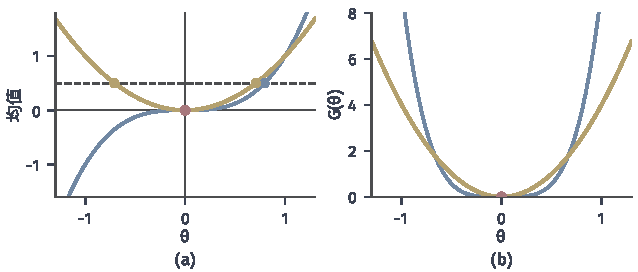
\includegraphics[width=108mm]{figures/07-probability/07-distribution-optimization/matplotlib/igeo-cubic-information/figure.pdf}
  \caption{两个单参数高斯族$\mathcal{N}(\theta^{3},1)$（蓝）与$\mathcal{N}(\theta^{2},1)$（黄）。(a)均值随$\theta$的变化，深灰虚线为均值$0.5$，与蓝线交于一点、与黄线交于两点；(b)Fisher信息$9\theta^{4}$与$4\theta^{2}$。红点$\theta=0$处两者的信息都为零。}
  \label{fig:igeo-cubic-information}
\end{BookInlineFigure}

图~\ref{fig:igeo-cubic-information}把前两个族放在一起。三件事由此分开：参数冗余是整条方向上分布都不变，信息在那个方向上处处为零；局部一阶退化是某一点上分布的一阶变化消失，分布本身仍可辨识；全局可辨识则要求不同参数给出不同分布，它与某点的信息是否为零没有蕴含关系。后面凡是要对$\bm{G}(\bm{\theta})$求逆，都要另加它正定的假设，并在不满足时先弄清是哪一种情形。


\section{分布变化的局部尺度}
\label{sec:igeo-local-scale}

Fisher信息是从得分的二阶矩定义的，它是否真的衡量了“分布变了多少”？章首的均值位移给出一个线索。由第~\ref{chap:distribution-comparison}章两个等方差高斯分布的KL公式，
\[
  D_{\mathrm{KL}}\bigl(\mathcal{N}(\mu,\sigma^{2})\Vert\mathcal{N}(\mu+\delta,\sigma^{2})\bigr)=\frac{\delta^{2}}{2\sigma^{2}}=\frac12\,G_{\mu\mu}\,\delta^{2},
\]
其中$G_{\mu\mu}=1/\sigma^{2}$是式~\eqref{eq:igeo-gauss-fisher}的第一个对角元。$\delta=0.5$时，$\sigma=0.5$与$\sigma=2$分别给出$0.5$与$1/32$，正是章首的两个数。这一节先证明在一般的正则族中，邻近分布间的KL散度在二阶意义下都是$\frac12\bm{\delta}^{\top}\bm{G}\bm{\delta}$；再换参数坐标，看矩阵怎样变，它所表示的局部变化又是否保持。

\subsection{KL的二阶展开}
\label{sec:igeo-kl-expansion}

展开$D_{\mathrm{KL}}(P_{\bm{\theta}}\Vert P_{\bm{\theta}+\bm{\delta}})$，就是对$\ln p_{\bm{\theta}+\bm{\delta}}(x)$在$\bm{\theta}$处作Taylor展开再取期望。一阶项的期望是得分的期望，为零；二阶项的期望涉及对数密度的Hessian矩阵。先把这个期望与Fisher信息联系起来。

\begin{lemma}[信息等式]
\label{lem:igeo-information-identity}
设分布族正则，对每个$x\in S$，$\bm{\theta}\mapsto p_{\bm{\theta}}(x)$二阶连续可微；在给定的$\bm{\theta}$处，$\int_{S}\lVert\nabla_{\bm{\theta}}^{2}p_{\bm{\theta}}\rVert\,\mathrm{d}\nu<\infty$，$\bm{G}(\bm{\theta})$有限，并且二阶导数也可以与积分交换：
\begin{equation}
  \int_{S}\nabla_{\bm{\theta}}^{2}p_{\bm{\theta}}\,\mathrm{d}\nu=\nabla_{\bm{\theta}}^{2}\int_{S}p_{\bm{\theta}}\,\mathrm{d}\nu=\bm{0}.
  \label{eq:igeo-second-exchange}
\end{equation}
则
\begin{equation}
  \mathbb{E}_{\bm{\theta}}\bigl[\nabla_{\bm{\theta}}^{2}\ln p_{\bm{\theta}}(X)\bigr]=-\bm{G}(\bm{\theta}).
  \label{eq:igeo-information-identity}
\end{equation}
\end{lemma}

\begin{proof}
在$S$上对式~\eqref{eq:igeo-score}的商再求一次导数，商的求导法则给出
\[
  \nabla_{\bm{\theta}}^{2}\ln p_{\bm{\theta}}=\frac{\nabla_{\bm{\theta}}^{2}p_{\bm{\theta}}}{p_{\bm{\theta}}}-\frac{\nabla_{\bm{\theta}}p_{\bm{\theta}}\,\nabla_{\bm{\theta}}p_{\bm{\theta}}^{\top}}{p_{\bm{\theta}}^{2}}=\frac{\nabla_{\bm{\theta}}^{2}p_{\bm{\theta}}}{p_{\bm{\theta}}}-\bm{s}_{\bm{\theta}}\bm{s}_{\bm{\theta}}^{\top}.
\]
两项在$P_{\bm{\theta}}$下都可积：第一项的期望是$\int_{S}\nabla_{\bm{\theta}}^{2}p_{\bm{\theta}}\,\mathrm{d}\nu$，由式~\eqref{eq:igeo-second-exchange}为零矩阵；第二项的期望是$\bm{G}(\bm{\theta})$。相减即得式~\eqref{eq:igeo-information-identity}。
\end{proof}

式~\eqref{eq:igeo-information-identity}给出Fisher信息的第二种算法：对数密度的平均曲率取负号。在对数密度的峰附近，曲率越大，峰越尖，参数稍变，对数密度就下降得越多。下面的定理把这两种描述合成KL散度的局部形状。对数密度在参数$\bm{\theta}'$处的Hessian矩阵记为
\[
  \bm{H}_{\bm{\theta}'}(x)=\nabla_{\bm{\theta}}^{2}\ln p_{\bm{\theta}'}(x).
\]

\begin{theorem}[KL散度的二阶展开]
\label{thm:igeo-kl-expansion}
设引理~\ref{lem:igeo-information-identity}的条件在$\bm{\theta}$处成立，并且存在$r>0$与函数$M\geq0$，使以$\bm{\theta}$为心、$r$为半径的闭球$B_r$含于$\Theta$，$\mathbb{E}_{\bm{\theta}}[M(X)]<\infty$，且对所有$\bm{\theta}'\in B_r$与$x\in S$，
\begin{equation}
  \lVert\bm{H}_{\bm{\theta}'}(x)\rVert\leq M(x),
  \label{eq:igeo-hessian-control}
\end{equation}
这里$\lVert\cdot\rVert$为矩阵的谱范数。则当$\bm{\delta}\to\bm{0}$时
\begin{equation}
  D_{\mathrm{KL}}(P_{\bm{\theta}}\Vert P_{\bm{\theta}+\bm{\delta}})=\frac12\,\bm{\delta}^{\top}\bm{G}(\bm{\theta})\bm{\delta}+o(\lVert\bm{\delta}\rVert_2^{2}).
  \label{eq:igeo-kl-expansion}
\end{equation}
\end{theorem}

\begin{proof}
设$\lVert\bm{\delta}\rVert_2<r$。两个分布有共同支撑$S$，$P_{\bm{\theta}}\ll P_{\bm{\theta}+\bm{\delta}}$，KL散度是对数密度比在$P_{\bm{\theta}}$下的期望，只要这个期望存在。

第一步，逐点展开。对固定的$x\in S$，函数$t\mapsto\ln p_{\bm{\theta}+t\bm{\delta}}(x)$在$[0,1]$上二阶连续可微，带积分余项的Taylor公式给出
\[
  \ln p_{\bm{\theta}+\bm{\delta}}(x)-\ln p_{\bm{\theta}}(x)=\bm{\delta}^{\top}\bm{s}_{\bm{\theta}}(x)+\int_{0}^{1}(1-t)\,\bm{\delta}^{\top}\bm{H}_{\bm{\theta}+t\bm{\delta}}(x)\bm{\delta}\,\mathrm{d}t .
\]

第二步，检查可积性。由式~\eqref{eq:igeo-hessian-control}，余项的绝对值不超过$\frac12\lVert\bm{\delta}\rVert_2^{2}M(x)$；$\bm{G}(\bm{\theta})$有限说明$\lVert\bm{s}_{\bm{\theta}}\rVert_2$平方可积，因而可积。所以左端在$P_{\bm{\theta}}$下可积，KL散度有限，并且
\[
  D_{\mathrm{KL}}(P_{\bm{\theta}}\Vert P_{\bm{\theta}+\bm{\delta}})=-\bm{\delta}^{\top}\mathbb{E}_{\bm{\theta}}[\bm{s}_{\bm{\theta}}]-\mathbb{E}_{\bm{\theta}}\Bigl[\int_{0}^{1}(1-t)\,\bm{\delta}^{\top}\bm{H}_{\bm{\theta}+t\bm{\delta}}\bm{\delta}\,\mathrm{d}t\Bigr].
\]

第三步，分出主项。由引理~\ref{lem:igeo-score-mean}，第一项为零。在第二项中加减$\bm{H}_{\bm{\theta}}$，并利用$\int_{0}^{1}(1-t)\,\mathrm{d}t=\frac12$与式~\eqref{eq:igeo-information-identity}，得到
\[
  D_{\mathrm{KL}}(P_{\bm{\theta}}\Vert P_{\bm{\theta}+\bm{\delta}})=\frac12\bm{\delta}^{\top}\bm{G}(\bm{\theta})\bm{\delta}-R(\bm{\delta}),
\]
其中
\[
  R(\bm{\delta})=\mathbb{E}_{\bm{\theta}}\Bigl[\int_{0}^{1}(1-t)\,\bm{\delta}^{\top}\bigl(\bm{H}_{\bm{\theta}+t\bm{\delta}}-\bm{H}_{\bm{\theta}}\bigr)\bm{\delta}\,\mathrm{d}t\Bigr].
\]

第四步，估计余项。对$0<\rho\leq r$，令
\[
  \omega_{\rho}(x)=\sup_{\lVert\bm{u}\rVert_2\leq\rho}\lVert\bm{H}_{\bm{\theta}+\bm{u}}(x)-\bm{H}_{\bm{\theta}}(x)\rVert .
\]
$\bm{H}$对参数连续，上确界可以只在有理点上取，所以$\omega_{\rho}$可测。于是
\[
  \lvert R(\bm{\delta})\rvert\leq\frac12\lVert\bm{\delta}\rVert_2^{2}\,\mathbb{E}_{\bm{\theta}}\bigl[\omega_{\lVert\bm{\delta}\rVert_2}(X)\bigr].
\]
由$\bm{H}$的连续性，$\rho\to0$时$\omega_{\rho}(x)\to0$对每个$x$成立；又$\omega_{\rho}\leq2M$，由控制收敛定理，$\mathbb{E}_{\bm{\theta}}[\omega_{\rho}]\to0$。所以$R(\bm{\delta})=o(\lVert\bm{\delta}\rVert_2^{2})$。
\end{proof}

定理中各条件的分工如下。共同支撑使对数密度比有定义；二阶可微与积分交换给出信息等式；控制函数$M$让余项能够在期望下一致地变小。KL散度用自然对数定义时系数是$\frac12$；若以比特计，用$\log_2$代替$\ln$，右端要再除以$\ln2$。交换两个分布的位置，在邻域内一致的控制条件下也得到同样的二阶项：把展开点换成$\bm{\theta}+\bm{\delta}$重复上面的论证，再用$\bm{G}$的连续性把$\bm{G}(\bm{\theta}+\bm{\delta})$换成$\bm{G}(\bm{\theta})$。KL散度本身不对称，但这种不对称从三阶才开始显现。

\paragraph{对数方差坐标中的检验}
取均值为零的高斯族$\mathcal{N}(0,v)$，用$\tau=\ln v$作参数。由第~\ref{chap:distribution-comparison}章的高斯KL公式，把$v'=v\mathrm{e}^{\Delta}$代入，得到
\begin{equation}
  D_{\mathrm{KL}}\bigl(\mathcal{N}(0,v)\Vert\mathcal{N}(0,v\mathrm{e}^{\Delta})\bigr)=\frac12\ln\mathrm{e}^{\Delta}+\frac{v}{2v\mathrm{e}^{\Delta}}-\frac12=\frac12\bigl(\Delta+\mathrm{e}^{-\Delta}-1\bigr).
  \label{eq:igeo-logvar-kl}
\end{equation}
结果只依赖于$\Delta$，与起点$v$无关，这就是章首所说对数方差坐标的特点。把指数函数的展开
\[
  \mathrm{e}^{-\Delta}=1-\Delta+\frac{\Delta^{2}}{2}-\frac{\Delta^{3}}{6}+\cdots
\]
代入，得到
\[
  D_{\mathrm{KL}}=\frac{\Delta^{2}}{4}-\frac{\Delta^{3}}{12}+\cdots .
\]
定理~\ref{thm:igeo-kl-expansion}预言二阶项是$\frac12G_{\tau\tau}\Delta^{2}$，所以这一坐标下$G_{\tau\tau}=\frac12$；下一小节将用坐标变换公式独立地得到这个值。

图~\ref{fig:igeo-kl-quadratic}比较两个方向的精确KL与二次近似$\Delta^{2}/4$。$\Delta=0.5$时，两个方向分别是$0.053$与$0.074$，二次近似为$0.0625$，三者相差不到三成；$\Delta=2$时，两个方向分别是$0.568$与$2.19$，二次近似为$1$，已经失去意义。二次型只描述一点附近的变化，它不是全局的距离公式。

\begin{BookInlineFigure}
  \centering
  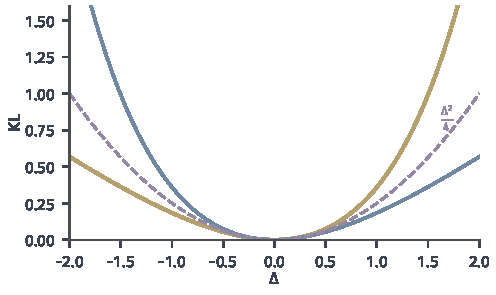
\includegraphics[width=84mm]{figures/07-probability/07-distribution-optimization/matplotlib/igeo-kl-quadratic/figure.pdf}
  \caption{对数方差坐标$\tau=\ln\sigma^{2}$中位移$\Delta$引起的KL散度。蓝线：$D_{\mathrm{KL}}(P_{\tau}\Vert P_{\tau+\Delta})=\frac12(\Delta+\mathrm{e}^{-\Delta}-1)$；黄线：反方向$\frac12(\mathrm{e}^{\Delta}-\Delta-1)$；紫色虚线：二次近似$\frac12G_{\tau\tau}\Delta^{2}=\Delta^{2}/4$。三条曲线在$\Delta=0$附近重合，远处分开。}
  \label{fig:igeo-kl-quadratic}
\end{BookInlineFigure}

局部非退化也推不出全局的参数唯一。在$\mathcal{N}(\theta^{2},1)$中取$\theta=1$，$G(1)=4>0$，二次近似说位移$\delta=-2$应带来约$\frac12\cdot4\cdot4=8$的KL散度；而$\theta+\delta=-1$与$\theta=1$给出同一个分布，真实的KL散度为零。展开只对足够小的$\bm{\delta}$成立，“足够小”有多小，取决于族在这一点附近的形状。

\paragraph{Fisher椭圆}
在二维参数空间中，位移的集合
\[
  \Bigl\{\bm{\delta}:\frac12\bm{\delta}^{\top}\bm{G}(\bm{\theta})\bm{\delta}=\varepsilon\Bigr\}
\]
放在$\bm{\theta}$处是一个以$\bm{\theta}$为中心的椭圆。局部看，椭圆上每个点代表的邻近分布与中心分布的KL散度都约为$\varepsilon$。高斯族在$(\mu,\sigma)$坐标下，由式~\eqref{eq:igeo-gauss-fisher}，椭圆沿$\mu$方向的半轴为$\sigma\sqrt{2\varepsilon}$，沿$\sigma$方向的半轴为$\sigma\sqrt{\varepsilon}$。

图~\ref{fig:igeo-fisher-ellipses}把这些椭圆画在$(\mu,\sigma)$半平面上。同一行的椭圆一样大：平移不改变局部尺度。越靠近$\sigma=0$，椭圆越小：分布越窄，参数只要稍动就造成同样大小的变化。每个椭圆横向比纵向宽$\sqrt2$倍：同样的KL预算下，均值可以比$\sigma$多动一些。把这些椭圆当作各点的“单位圆”，参数平面就带上了一把随位置变化的尺子。

\begin{BookInlineFigure}
  \centering
  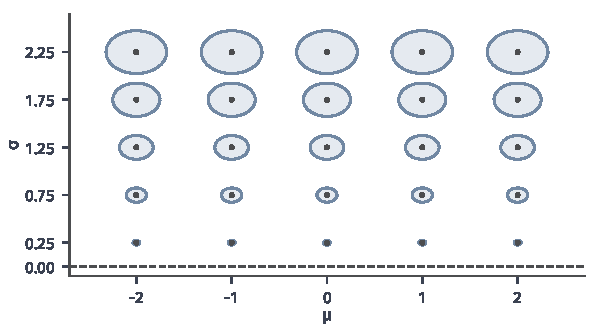
\includegraphics[width=100mm]{figures/07-probability/07-distribution-optimization/matplotlib/igeo-fisher-ellipses/figure.pdf}
  \caption{高斯族在$(\mu,\sigma)$半平面上的Fisher椭圆$\frac12\bm{\delta}^{\top}\bm{G}\bm{\delta}=0.01$。中心为深灰点，$\sigma$取$0.25,0.75,\dots,2.25$，$\mu$取$-2,\dots,2$；半轴为$0.141\sigma$（$\mu$方向）与$0.1\sigma$（$\sigma$方向）。深灰虚线$\sigma=0$不属于参数集合。}
  \label{fig:igeo-fisher-ellipses}
\end{BookInlineFigure}

\subsection{坐标变换}
\label{sec:igeo-coordinates}

同一个高斯族可以用$(\mu,\sigma)$、$(\mu,\sigma^{2})$、$(\mu,\ln\sigma^{2})$或第~\ref{chap:distribution-families}章的自然参数来编号。章首的例子已经显示，同样增加$0.1$，在方差坐标中引起的KL随起点变化，在对数方差坐标中则不变。分布族没有变，变的只是编号的方式。Fisher信息的数值随编号而变，这在章首已经看到；问题是它所表示的“局部变化有多大”是否也依赖于编号。

设$\Xi\subset\mathbb{R}^{k}$是开集，$\bm{\varphi}:\Xi\to\Theta$是连续可微的双射，其逆也连续可微，Jacobian矩阵
\[
  \bm{J}(\bm{\xi})=\frac{\partial\bm{\theta}}{\partial\bm{\xi}}\in\mathbb{R}^{k\times k},\qquad J_{i,j}=\frac{\partial\theta_{i}}{\partial\xi_{j}},
\]
处处非奇异。新坐标下的族是$q_{\bm{\xi}}=p_{\bm{\varphi}(\bm{\xi})}$。它仍是正则族：支撑不变，逐点可微由链式法则得到，而在$\bm{\xi}$的紧邻域上$\bm{J}$有界，原来的控制函数乘以这个界仍然可积。

\begin{theorem}[得分与Fisher信息的坐标变换]
\label{thm:igeo-reparam}
在上述设定下，记$\bm{\theta}=\bm{\varphi}(\bm{\xi})$，$\bm{J}=\bm{J}(\bm{\xi})$，则
\begin{equation}
  \bm{s}^{\Xi}_{\bm{\xi}}(x)=\bm{J}^{\top}\bm{s}_{\bm{\theta}}(x),\qquad
  \bm{G}^{\Xi}(\bm{\xi})=\bm{J}^{\top}\bm{G}(\bm{\theta})\bm{J}.
  \label{eq:igeo-reparam}
\end{equation}
对任意$\mathrm{d}\bm{\xi}\in\mathbb{R}^{k}$，令$\mathrm{d}\bm{\theta}=\bm{J}\,\mathrm{d}\bm{\xi}$，则
\begin{equation}
  \mathrm{d}\bm{\xi}^{\top}\bm{G}^{\Xi}(\bm{\xi})\,\mathrm{d}\bm{\xi}=\mathrm{d}\bm{\theta}^{\top}\bm{G}(\bm{\theta})\,\mathrm{d}\bm{\theta}.
  \label{eq:igeo-invariant-form}
\end{equation}
\end{theorem}

\begin{proof}
由链式法则，对每个$j$，
\[
  \frac{\partial}{\partial\xi_{j}}\ln p_{\bm{\varphi}(\bm{\xi})}(x)=\sum_{i=1}^{k}\frac{\partial\ln p_{\bm{\theta}}(x)}{\partial\theta_{i}}\,\frac{\partial\theta_{i}}{\partial\xi_{j}},
\]
写成向量就是式~\eqref{eq:igeo-reparam}的第一式。$\bm{J}$不随$x$变化，代入式~\eqref{eq:igeo-fisher}，
\[
  \bm{G}^{\Xi}(\bm{\xi})=\mathbb{E}\bigl[\bm{J}^{\top}\bm{s}_{\bm{\theta}}\bm{s}_{\bm{\theta}}^{\top}\bm{J}\bigr]=\bm{J}^{\top}\bm{G}(\bm{\theta})\bm{J}.
\]
最后，
\[
  \mathrm{d}\bm{\xi}^{\top}\bm{J}^{\top}\bm{G}(\bm{\theta})\bm{J}\,\mathrm{d}\bm{\xi}=(\bm{J}\,\mathrm{d}\bm{\xi})^{\top}\bm{G}(\bm{\theta})(\bm{J}\,\mathrm{d}\bm{\xi}),
\]
即式~\eqref{eq:igeo-invariant-form}。
\end{proof}

式~\eqref{eq:igeo-invariant-form}的含义是：$\mathrm{d}\bm{\xi}$与$\mathrm{d}\bm{\theta}=\bm{J}\,\mathrm{d}\bm{\xi}$是同一个无穷小位移在两套坐标中的分量。它们的数字不同，矩阵也不同，但二次型给出同一个值，而由定理~\ref{thm:igeo-kl-expansion}，这个值的一半正是该位移引起的局部KL。改变的是记录方式，不变的是分布本身的局部变化。

\paragraph{方差与对数方差}
在$\mathcal{N}(0,v)$中，$\ln p_{v}(x)=-\frac12\ln(2\pi v)-\frac{x^{2}}{2v}$，于是
\[
  s_{v}(x)=-\frac1{2v}+\frac{x^{2}}{2v^{2}}=\frac{x^{2}-v}{2v^{2}} .
\]
$X^{2}$的方差是$2v^{2}$，所以
\[
  G_{vv}=\frac{\operatorname{Var}(X^{2})}{4v^{4}}=\frac{2v^{2}}{4v^{4}}=\frac1{2v^{2}}.
\]
改用$\tau=\ln v$，$v=\mathrm{e}^{\tau}$，$J=\mathrm{d}v/\mathrm{d}\tau=v$，由式~\eqref{eq:igeo-reparam}，
\[
  G_{\tau\tau}=v^{2}\cdot\frac{1}{2v^{2}}=\frac12 ,
\]
与上一小节由KL展开读出的系数一致。

在$v=4$处取$\Delta v=0.4$，对应$\Delta\tau=\ln1.1\approx0.0953$，一阶近似为$0.1$。两套坐标下的二次型分别是
\[
  \frac12\cdot\frac1{32}\cdot0.4^{2}=0.0025,\qquad\frac12\cdot\frac12\cdot0.1^{2}=0.0025,
\]
完全相等；精确的KL为$0.0022$。而两个位移的欧氏长度一个是$0.4$，一个约是$0.1$。图~\ref{fig:igeo-coordinate-rulers}画出$v=0.5,1,2,4$四处局部KL不超过$0.01$的参数区间：在$v$轴上，区间长度与$v$成正比；在$\tau$轴上，四段一样长。

\begin{BookInlineFigure}
  \centering
  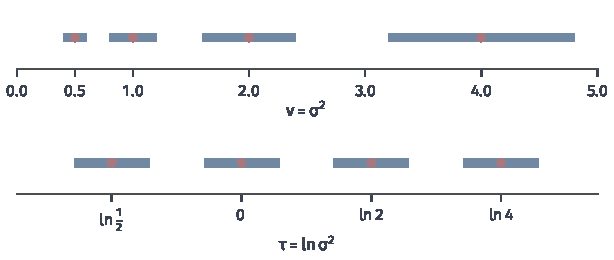
\includegraphics[width=104mm]{figures/07-probability/07-distribution-optimization/matplotlib/igeo-coordinate-rulers/figure.pdf}
  \caption{$\mathcal{N}(0,v)$在$v=0.5,1,2,4$（红点）处满足$\frac12G\,d^{2}\leq0.01$的参数区间（蓝色粗线）。上：方差坐标$v$，半长$0.2v$；下：对数方差坐标$\tau=\ln v$，半长都是$0.2$。两行对应的是同一组分布区间。}
  \label{fig:igeo-coordinate-rulers}
\end{BookInlineFigure}

\paragraph{二维的例子}
把均值加进来。在$(\mu,v)$坐标下，同样的计算给出
\[
  \bm{G}(\mu,v)=\begin{bmatrix}1/v&0\\0&1/(2v^{2})\end{bmatrix},\qquad
  \bm{G}(\mu,\tau)=\begin{bmatrix}1/v&0\\0&1/2\end{bmatrix}.
\]
在$\mathcal{N}(1,4)$处取$(\mu,\tau)$坐标中的位移$(0.6,\ 0.566)$，它满足$\frac12(0.25\cdot0.36+0.5\cdot0.32)=0.125$。换到$(\mu,v)$坐标，$\mathrm{d}v=v\,\mathrm{d}\tau$，位移变为$(0.6,\ 2.263)$，二次型为
\[
  \frac12\Bigl(\frac14\cdot0.36+\frac1{32}\cdot5.12\Bigr)=\frac12(0.09+0.16)=0.125 .
\]
图~\ref{fig:igeo-tangent-ellipses}中，绿色箭头在两张图里的分量相差约四倍，但箭头都恰好落在各自的椭圆$\frac12\bm{\delta}^{\top}\bm{G}\bm{\delta}=0.125$上。

\begin{BookInlineFigure}
  \centering
  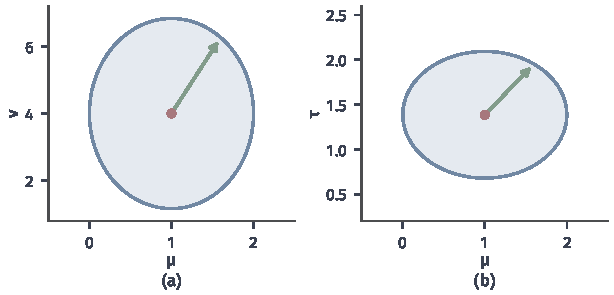
\includegraphics[width=104mm]{figures/07-probability/07-distribution-optimization/matplotlib/igeo-tangent-ellipses/figure.pdf}
  \caption{同一个位移在两套坐标中的表示，中心为$\mathcal{N}(1,4)$（红点）。(a)$(\mu,v)$坐标；(b)$(\mu,\tau)$坐标，$\tau=\ln v$。蓝色椭圆为$\frac12\bm{\delta}^{\top}\bm{G}\bm{\delta}=0.125$，绿色箭头分别是$(0.6,\,2.263)$与$(0.6,\,0.566)$，两者表示同一个位移，都落在椭圆上。两图纵轴的单位不同。}
  \label{fig:igeo-tangent-ellipses}
\end{BookInlineFigure}

\paragraph{几何的说法}
把每一种参数化看成分布族上的一张坐标卡，坐标之间的转换就是流形的坐标变换，无穷小位移就是切向量，它的分量按$\bm{J}$变换，这些概念可参考\BookChapterRef{chap:manifold-basics}{卷四第24章“流形的基本概念”}。式~\eqref{eq:igeo-invariant-form}说明，
\[
  \langle\bm{a},\bm{b}\rangle_{\bm{G}}=\bm{a}^{\top}\bm{G}(\bm{\theta})\bm{b}
\]
是切向量之间不依赖坐标的对称双线性形式。当$\bm{G}$处处正定且光滑变化时，它是参数流形上的一个Riemann度量，称为\term{Fisher度量}（Fisher metric），一般定义可参考\BookChapterRef{chap:riemannian-geometry}{卷四第27章“黎曼几何”}。

这个说法也标出了本节结论的边界。坐标变换下保持的是切向量的长度，即局部变化的大小；矩阵的元素、参数位移的欧氏长度都不保持。在$\bm{G}$退化的点，二次型只是半正定的，不能当作度量，需要先按第~\ref{sec:igeo-fisher}节的办法辨认退化的来源。


\section{指数族的坐标}
\label{sec:igeo-exponential}

前两节的每一步都要单独核验：积分能否与求导交换，得分是否平方可积，Hessian有没有可积的控制。指数族里这些检查都可以一次完成，而且所有的量都由一个函数——对数配分函数——决定。第~\ref{chap:distribution-families}章已经建立了下面的事实：指数族
\[
  p_{\bm{\theta}}(x)=h(x)\exp\bigl(\langle\bm{\theta},\bm{T}(x)\rangle-A(\bm{\theta})\bigr)
\]
相对参考测度$\nu$的所有成员有共同支撑$\{h>0\}$；在自然参数域$\Theta$的内点，$A$无穷次可微，$\bm{T}$的各阶矩有限，并且
\[
  \nabla A(\bm{\theta})=\mathbb{E}_{\bm{\theta}}[\bm{T}],\qquad\nabla^{2}A(\bm{\theta})=\operatorname{Cov}_{\bm{\theta}}(\bm{T}).
\]
在最小表示的正则指数族中，均值映射$\bm{m}=\nabla A$是$\Theta$到开集$\mathcal{M}^{\circ}$的双射，逆映射连续可微。

这一节用这些结论计算得分、Fisher信息与局部KL，并说明自然参数与均值参数两套坐标怎样互相转换。

\paragraph{得分与信息}
在自然参数域的内点，对数密度是$\ln h(x)+\langle\bm{\theta},\bm{T}(x)\rangle-A(\bm{\theta})$，对$\bm{\theta}$求导得到
\begin{equation}
  \bm{s}_{\bm{\theta}}(x)=\bm{T}(x)-\nabla A(\bm{\theta})=\bm{T}(x)-\mathbb{E}_{\bm{\theta}}[\bm{T}].
  \label{eq:igeo-expfam-score}
\end{equation}
得分就是自然统计量减去它的均值，期望为零不需要另外证明。它的协方差就是$\bm{T}$的协方差，于是
\begin{equation}
  \bm{G}(\bm{\theta})=\operatorname{Cov}_{\bm{\theta}}(\bm{T})=\nabla^{2}A(\bm{\theta}).
  \label{eq:igeo-expfam-fisher}
\end{equation}
再求一次导数，对数密度的Hessian是$-\nabla^{2}A(\bm{\theta})$，它不依赖$x$。所以信息等式~\eqref{eq:igeo-information-identity}直接成立；$\nabla^{2}A$连续，在内点的闭球邻域上有界，定理~\ref{thm:igeo-kl-expansion}所需的控制函数可以取常数。正则指数族因此在参数域的每一点都满足前两节的全部条件。

单参数的例子可以从第~\ref{chap:distribution-families}章已算出的导数直接读出。Bernoulli族的自然参数是$\theta=\ln\frac{p}{1-p}$，$G(\theta)=A''(\theta)=p(1-p)$。$\{0,1,2\}$上的倾斜族$p_{\theta}(x)\propto\mathrm{e}^{\theta x}$在$\theta=\ln2$处是$(\frac17,\frac27,\frac47)$，均值为$\frac{10}{7}$，于是
\[
  G(\ln2)=A''(\ln2)=\frac{26}{49}.
\]

高斯族$\mathcal{N}(\mu,\sigma^{2})$取$\bm{T}(x)=(x,x^{2})$，自然参数为$(\mu/\sigma^{2},\,-1/(2\sigma^{2}))$，Fisher信息是$X$与$X^{2}$的协方差矩阵。需要用到高斯分布的三阶与四阶矩：
\[
  \mathbb{E}[X^{3}]=\mu^{3}+3\mu\sigma^{2},\qquad\mathbb{E}[X^{4}]=\mu^{4}+6\mu^{2}\sigma^{2}+3\sigma^{4}.
\]
由此得到
\[
  \operatorname{Cov}(X,X^{2})=\mathbb{E}[X^{3}]-\mu(\mu^{2}+\sigma^{2})=2\mu\sigma^{2},
\]
\[
  \operatorname{Var}(X^{2})=\mathbb{E}[X^{4}]-(\mu^{2}+\sigma^{2})^{2}=4\mu^{2}\sigma^{2}+2\sigma^{4}.
\]
于是自然参数坐标下
\begin{equation}
  \bm{G}(\bm{\theta})=\begin{bmatrix}\sigma^{2}&2\mu\sigma^{2}\\2\mu\sigma^{2}&4\mu^{2}\sigma^{2}+2\sigma^{4}\end{bmatrix}.
  \label{eq:igeo-gauss-natural-fisher}
\end{equation}

例如$\mathcal{N}(1,4)$的自然参数是$(0.25,\,-0.125)$，代入式~\eqref{eq:igeo-gauss-natural-fisher}，信息矩阵为
\[
  \bm{G}=\begin{bmatrix}4&8\\8&48\end{bmatrix}.
\]
它不是对角阵：在自然参数坐标下，两个分量的变化互相纠缠。这个矩阵会在第~\ref{sec:igeo-natural-gradient}节与第~\ref{sec:igeo-implementation}节反复用到。

\paragraph{KL散度是Bregman距离}
在指数族中，KL散度有不必取极限的精确表示。设$\bm{\theta},\bm{\theta}'\in\Theta$都是内点。两个对数密度之差不含$h$：
\[
  \ln\frac{p_{\bm{\theta}}(x)}{p_{\bm{\theta}'}(x)}=\langle\bm{\theta}-\bm{\theta}',\bm{T}(x)\rangle-A(\bm{\theta})+A(\bm{\theta}').
\]
在$P_{\bm{\theta}}$下取期望，$\bm{T}$的期望换成$\nabla A(\bm{\theta})$，得到
\begin{equation}
  D_{\mathrm{KL}}(P_{\bm{\theta}}\Vert P_{\bm{\theta}'})=A(\bm{\theta}')-A(\bm{\theta})-\langle\nabla A(\bm{\theta}),\bm{\theta}'-\bm{\theta}\rangle .
  \label{eq:igeo-expfam-bregman}
\end{equation}

右端是凸函数$A$在$\bm{\theta}'$处的值减去它在$\bm{\theta}$处的切平面的值，称为由$A$生成的\term{Bregman距离}（Bregman distance）。它非负，因为凸函数在切平面之上；它一般不对称，也不满足三角不等式，“距离”只是习惯的叫法。把$A$在$\bm{\theta}$处作二阶Taylor展开，切平面以上的部分是
\[
  \frac12(\bm{\theta}'-\bm{\theta})^{\top}\nabla^{2}A(\bm{\theta})(\bm{\theta}'-\bm{\theta})+o(\lVert\bm{\theta}'-\bm{\theta}\rVert_2^{2}),
\]
由式~\eqref{eq:igeo-expfam-fisher}，这正是定理~\ref{thm:igeo-kl-expansion}在指数族中的形式。

在倾斜族上算一个例子。取$\theta=\ln2$，$\theta'=0$，后者是均匀分布$(\frac13,\frac13,\frac13)$。这个族的对数配分函数是$\ln(1+\mathrm{e}^{\theta}+\mathrm{e}^{2\theta})$，于是$A(0)=\ln3$，$A(\ln2)=\ln7$，代入式~\eqref{eq:igeo-expfam-bregman}，
\[
  D_{\mathrm{KL}}(P_{\ln2}\Vert P_{0})=\ln3-\ln7+\frac{10}{7}\ln2\approx0.1429 .
\]
直接按定义逐项求和，
\[
  \frac17\ln\frac37+\frac27\ln\frac67+\frac47\ln\frac{12}7\approx-0.1210-0.0440+0.3080=0.1430,
\]
在四位小数的舍入范围内一致。二次近似给出$\frac12\cdot\frac{26}{49}\cdot(\ln2)^{2}\approx0.1275$，相差约一成，因为$\ln2\approx0.69$已不算很小的位移。图~\ref{fig:igeo-bregman}(a)中的红色竖线就是这个间隙。

\paragraph{均值坐标}
第~\ref{chap:distribution-families}章说明，在最小表示的正则指数族中，也可以用均值参数$\bm{m}=\mathbb{E}_{\bm{\theta}}[\bm{T}]$给分布编号。均值映射$\bm{m}=\nabla A(\bm{\theta})$的Jacobian矩阵是
\[
  \frac{\partial\bm{m}}{\partial\bm{\theta}}=\nabla^{2}A(\bm{\theta})=\bm{G}(\bm{\theta}),
\]
在最小表示下它正定。由反函数定理（见\BookChapterRef{chap:implicit-inverse-functions}{卷二第22章“隐函数与反函数”}），逆映射$\bm{m}\mapsto\bm{\theta}(\bm{m})$的Jacobian是$\bm{G}(\bm{\theta})^{-1}$。在定理~\ref{thm:igeo-reparam}中取新坐标$\bm{\xi}=\bm{m}$，Jacobian就是$\bm{G}(\bm{\theta})^{-1}$，得到均值坐标下的Fisher信息
\begin{equation}
  \bm{G}^{\mathcal{M}}(\bm{m})=\bm{G}(\bm{\theta})^{-1}\bm{G}(\bm{\theta})\bm{G}(\bm{\theta})^{-1}=\bm{G}(\bm{\theta})^{-1}.
  \label{eq:igeo-mean-fisher}
\end{equation}
同一个Jacobian矩阵既是坐标转换的导数，又是自然坐标中的Fisher信息；而两套坐标中的Fisher信息互为逆矩阵。

Bernoulli族可以直接核对。用$p$作参数，$\ln p_{p}(x)=x\ln p+(1-x)\ln(1-p)$，得分是$\frac{x}{p}-\frac{1-x}{1-p}$，于是
\[
  G^{\mathcal{M}}(p)=p\cdot\frac{1}{p^{2}}+(1-p)\cdot\frac{1}{(1-p)^{2}}=\frac1{p(1-p)},
\]
恰是$G(\theta)=p(1-p)$的倒数。取$\theta=\ln3$，$p=\frac34$，两个值分别是$\frac{3}{16}$与$\frac{16}{3}$。图~\ref{fig:igeo-dual-coordinates}把两条曲线并排画出：自然坐标中，$\lvert\theta\rvert$很大时信息趋于零，一大段参数只对应很小的分布变化；均值坐标中，$p$接近$0$或$1$时信息趋于无穷，$p$稍动，分布的相对变化就很大。两种说法描述的是同一件事。

\begin{BookInlineFigure}
  \centering
  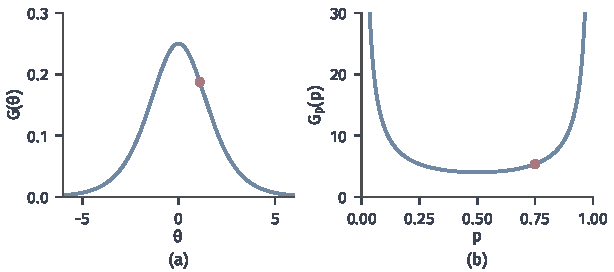
\includegraphics[width=104mm]{figures/07-probability/07-distribution-optimization/matplotlib/igeo-dual-coordinates/figure.pdf}
  \caption{Bernoulli族在两套坐标下的Fisher信息。(a)自然参数$\theta=\ln\frac{p}{1-p}$，$G(\theta)=p(1-p)$；(b)均值参数$p$，$G_{p}(p)=1/(p(1-p))$。红点对应同一个分布$\theta=\ln3$、$p=\frac34$，两值$\frac{3}{16}$与$\frac{16}{3}$互为倒数。}
  \label{fig:igeo-dual-coordinates}
\end{BookInlineFigure}

\paragraph{对偶势函数}
自然坐标有势函数$A$，它的梯度给出均值坐标、Hessian给出Fisher信息。均值坐标也有对应的势函数。在$\mathcal{M}^{\circ}$上令
\begin{equation}
  A^{*}(\bm{m})=\langle\bm{\theta}(\bm{m}),\bm{m}\rangle-A(\bm{\theta}(\bm{m})).
  \label{eq:igeo-dual-potential}
\end{equation}
$A$严格凸，$\bm{\theta}(\bm{m})$是$\langle\bm{\theta},\bm{m}\rangle-A(\bm{\theta})$对$\bm{\theta}$的唯一驻点，因而是最大点，所以
\[
  A^{*}(\bm{m})=\sup_{\bm{\theta}\in\Theta}\bigl\{\langle\bm{\theta},\bm{m}\rangle-A(\bm{\theta})\bigr\},
\]
即$A$的\term{凸共轭}（convex conjugate）在$\mathcal{M}^{\circ}$上的值。它也有概率含义：由式~\eqref{eq:igeo-dual-potential}，$A^{*}(\bm{m})$是$\ln(p_{\bm{\theta}}/h)$在$P_{\bm{\theta}}$下的期望；在有限集上取计数测度且$h=1$时，$A^{*}(\bm{m})$就是$P_{\bm{\theta}}$的负熵$-H(P_{\bm{\theta}})$。

对$\bm{m}$求导，记$\bm{K}=\partial\bm{\theta}/\partial\bm{m}$，
\[
  \nabla A^{*}(\bm{m})=\bm{\theta}+\bm{K}^{\top}\bm{m}-\bm{K}^{\top}\nabla A(\bm{\theta})=\bm{\theta}(\bm{m}),
\]
因为$\nabla A(\bm{\theta})=\bm{m}$，后两项抵消。再求一次导数，
\[
  \nabla^{2}A^{*}(\bm{m})=\frac{\partial\bm{\theta}}{\partial\bm{m}}=\bm{G}(\bm{\theta})^{-1}=\bm{G}^{\mathcal{M}}(\bm{m}).
\]
两个势函数的梯度把两套坐标互相转换，Hessian分别是各自坐标中的Fisher信息，所以这两套坐标常称为一对\term{对偶坐标}（dual coordinates）。

KL散度在均值坐标中也是Bregman距离，只是生成函数换成$A^{*}$，参数的先后次序反过来。由式~\eqref{eq:igeo-dual-potential}，
\[
  A(\bm{\theta})=\langle\bm{\theta},\bm{m}\rangle-A^{*}(\bm{m}),\qquad A(\bm{\theta}')=\langle\bm{\theta}',\bm{m}'\rangle-A^{*}(\bm{m}').
\]
把它们代入式~\eqref{eq:igeo-expfam-bregman}，$\langle\bm{\theta},\bm{m}\rangle$两项抵消，再用$\nabla A^{*}(\bm{m}')=\bm{\theta}'$，得到
\begin{equation}
  D_{\mathrm{KL}}(P_{\bm{\theta}}\Vert P_{\bm{\theta}'})=A^{*}(\bm{m})-A^{*}(\bm{m}')-\langle\nabla A^{*}(\bm{m}'),\bm{m}-\bm{m}'\rangle .
  \label{eq:igeo-dual-bregman}
\end{equation}

在倾斜族的例子中，$m=\frac{10}{7}$，$m'=1$，$(A^{*})'(1)=\theta'=0$，式~\eqref{eq:igeo-dual-bregman}化为
\[
  A^{*}\bigl(\tfrac{10}{7}\bigr)-A^{*}(1)=-H\bigl(\tfrac17,\tfrac27,\tfrac47\bigr)+\ln3\approx0.1429,
\]
与前面的结果相同。图~\ref{fig:igeo-bregman}把两种表示并排画出：同一个KL散度，左边是$A$在$\theta'$处高出切线的量，右边是$A^{*}$在$m$处高出切线的量。

\begin{BookInlineFigure}
  \centering
  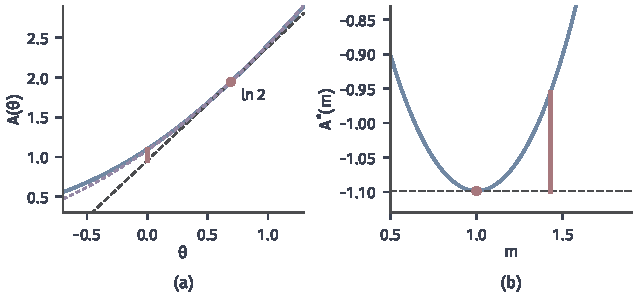
\includegraphics[width=108mm]{figures/07-probability/07-distribution-optimization/matplotlib/igeo-bregman/figure.pdf}
  \caption{$\{0,1,2\}$上倾斜族$p_{\theta}(x)\propto\mathrm{e}^{\theta x}$中$D_{\mathrm{KL}}(P_{\ln2}\Vert P_{0})\approx0.1429$的两种表示（红色竖线）。(a)对数配分函数$A(\theta)$（蓝），深灰虚线为$\theta=\ln2$处的切线（斜率$\frac{10}{7}$），紫色点线为切线加二次项$\frac12\cdot\frac{26}{49}(\theta-\ln2)^{2}$；(b)对偶势函数$A^{*}(m)$（蓝），深灰虚线为$m'=1$处的切线（斜率$0$）。}
  \label{fig:igeo-bregman}
\end{BookInlineFigure}

\paragraph{可逆性失效的情形}
两套坐标的对应依赖两个前提：表示是最小的，参数是自然参数域的内点。去掉任何一个，上面的公式都会出问题。

第一种情形是冗余统计量。Bernoulli族用$x=0$与$x=1$两个示性函数作统计量时，两个分量之和恒为$1$，协方差矩阵
\[
  \bm{G}=\operatorname{Cov}(\bm{T})=p(1-p)\begin{bmatrix}1&-1\\-1&1\end{bmatrix}
\]
处处奇异，零空间沿$(1,1)$方向。沿这个方向改变自然参数，分布不变；均值$(1-p,\,p)$只落在一条直线上，均值映射的像不是$\mathbb{R}^{2}$中的开集，无从定义逆映射。去掉一个统计量回到最小表示，就回到上一段的一维情形。

第二种情形是边界参数。第~\ref{chap:distribution-families}章中$(0,\infty)$上$h(x)=(1+x)^{-2}$、$T(x)=x$的族，参数域是$(-\infty,0]$，边界点$\theta=0$属于参数域，但那里$T$的均值为无穷，得分$T-\mathbb{E}[T]$没有定义，Fisher信息与局部展开都无从谈起。即使边界点不属于参数域，靠近边界时坐标也会失衡：在Bernoulli族中，$\theta\to\pm\infty$时$G(\theta)\to0$，而$p\to0$或$1$时$G^{\mathcal{M}}(p)\to\infty$，族外的点质量$\delta_0$、$\delta_1$不对应任何有限的坐标。


\section{自然梯度}
\label{sec:igeo-natural-gradient}

第~\ref{chap:distribution-approximation}章在参数族$\{Q_{\bm{\theta}}\}$中逼近目标分布$\Pi$，目标函数$L(\bm{\theta})$例如取$D_{\mathrm{KL}}(Q_{\bm{\theta}}\Vert\Pi)$或$D_{\mathrm{KL}}(\Pi\Vert Q_{\bm{\theta}})$。这样的目标是参数的可微函数时，最直接的更新是沿负梯度走一步：$\bm{\theta}\leftarrow\bm{\theta}-\alpha\nabla_{\bm{\theta}}L$。上一节已经看到，参数的同一段欧氏长度在不同位置、不同坐标下代表的分布变化相差悬殊，按欧氏长度分配步伐并没有道理。更合理的问法是：在允许分布发生同样大小的局部变化时，哪个方向使目标下降最多？

本节用一个能手算的例子贯穿。目标分布取$\Pi=\mathcal{N}(0,1)$，候选族为$Q_{\mu,v}=\mathcal{N}(\mu,v)$，目标函数取第~\ref{chap:distribution-approximation}章的$D_{\mathrm{KL}}(Q\Vert\Pi)$。由第~\ref{chap:distribution-comparison}章的高斯KL公式，
\begin{equation}
  L(\mu,v)=-\frac12\ln v+\frac{v+\mu^{2}}{2}-\frac12 .
  \label{eq:igeo-running-objective}
\end{equation}
为了每一步都能核对，这里的目标就在候选族内，最优解$(\mu,v)=(0,1)$是已知的。起点取$\mathcal{N}(1,4)$，那里$L=-\ln2+2\approx1.3069$。

\subsection{受限的下降方向}
\label{sec:igeo-steepest}

记$\bm{g}=\nabla_{\bm{\theta}}L(\bm{\theta})$。参数走一小步$\bm{\delta}$，目标的一阶变化是$\langle\bm{g},\bm{\delta}\rangle$；由定理~\ref{thm:igeo-kl-expansion}，分布的局部变化约为Fisher二次型的一半。给定一个KL预算$\varepsilon>0$，考虑问题
\begin{equation}
  \min_{\bm{\delta}\in\mathbb{R}^{k}}\ \langle\bm{g},\bm{\delta}\rangle\qquad\text{s.t.}\qquad\frac12\bm{\delta}^{\top}\bm{G}(\bm{\theta})\bm{\delta}\leq\varepsilon .
  \label{eq:igeo-steepest-problem}
\end{equation}
若把约束换成$\lVert\bm{\delta}\rVert_2\leq r$，答案是$-\bm{g}$的方向，这就是普通梯度下降。约束换成Fisher二次型以后，答案改变。

\begin{theorem}[Fisher度量下的最速下降方向]
\label{thm:igeo-steepest}
设$\bm{G}=\bm{G}(\bm{\theta})$正定，$\bm{g}\neq\bm{0}$。则问题~\eqref{eq:igeo-steepest-problem}有唯一解
\begin{equation}
  \bm{\delta}^{*}=-\sqrt{\frac{2\varepsilon}{\bm{g}^{\top}\bm{G}^{-1}\bm{g}}}\;\bm{G}^{-1}\bm{g},
  \label{eq:igeo-steepest-solution}
\end{equation}
最小值为
\begin{equation}
  \langle\bm{g},\bm{\delta}^{*}\rangle=-\sqrt{2\varepsilon\,\bm{g}^{\top}\bm{G}^{-1}\bm{g}} .
  \label{eq:igeo-steepest-value}
\end{equation}
\end{theorem}

\begin{proof}
$\bm{G}$正定，所以
\[
  \langle\bm{a},\bm{b}\rangle_{\bm{G}}=\bm{a}^{\top}\bm{G}\bm{b}
\]
是$\mathbb{R}^{k}$上的内积，记相应的范数为$\lVert\cdot\rVert_{\bm{G}}$，约束就是$\bm{\delta}$的这个范数不超过$\sqrt{2\varepsilon}$。把目标的一阶变化写成这个内积：
\[
  \langle\bm{g},\bm{\delta}\rangle=(\bm{G}^{-1}\bm{g})^{\top}\bm{G}\bm{\delta}=\langle\bm{G}^{-1}\bm{g},\bm{\delta}\rangle_{\bm{G}} .
\]
由Cauchy--Schwarz不等式与约束，
\[
  \langle\bm{G}^{-1}\bm{g},\bm{\delta}\rangle_{\bm{G}}\geq-\lVert\bm{G}^{-1}\bm{g}\rVert_{\bm{G}}\,\lVert\bm{\delta}\rVert_{\bm{G}}\geq-\sqrt{\bm{g}^{\top}\bm{G}^{-1}\bm{g}}\,\sqrt{2\varepsilon},
\]
这里用了
\[
  \lVert\bm{G}^{-1}\bm{g}\rVert_{\bm{G}}^{2}=\bm{g}^{\top}\bm{G}^{-1}\bm{G}\bm{G}^{-1}\bm{g}=\bm{g}^{\top}\bm{G}^{-1}\bm{g}.
\]
第一个不等号取等当且仅当$\bm{\delta}=-c\,\bm{G}^{-1}\bm{g}$，$c\geq0$；第二个取等当且仅当$\bm{\delta}$落在椭圆的边界上。两者同时成立唯一确定$c$，即式~\eqref{eq:igeo-steepest-solution}；代入目标，得到式~\eqref{eq:igeo-steepest-value}。
\end{proof}

最优方向与预算$\varepsilon$无关，$\varepsilon$只决定走多远。这个方向值得单独命名。

\begin{definition}[自然梯度]
\label{def:igeo-natural-gradient}
设$\bm{G}(\bm{\theta})$正定。称
\begin{equation}
  \widetilde{\nabla}L(\bm{\theta})=\bm{G}(\bm{\theta})^{-1}\nabla_{\bm{\theta}}L(\bm{\theta})
  \label{eq:igeo-natural-gradient}
\end{equation}
为$L$在$\bm{\theta}$处的\term{自然梯度}（natural gradient）。
\end{definition}

普通梯度相当于假定参数空间各处、各方向的尺度都一样，相当于在一张比例尺处处相同的地图上找最陡的方向。Fisher信息说明这张地图的比例尺因地因向而异：$\bm{G}$大的方向，参数稍动分布就大变，走一小步就要花掉很多预算；$\bm{G}$小的方向，参数要走很远分布才有同样的变化。自然梯度用$\bm{G}^{-1}$把梯度重新分配到这些方向上，便宜的方向多走，贵的方向少走。类比的边界在于，Fisher尺度只在局部成立，它不告诉我们走远以后路面怎样。

\paragraph{例中的两个方向}
在$(\mu,v)$坐标下，由式~\eqref{eq:igeo-running-objective}，
\[
  \bm{g}=\Bigl(\mu,\ \frac12-\frac{1}{2v}\Bigr),\qquad\bm{G}=\begin{bmatrix}1/v&0\\0&1/(2v^{2})\end{bmatrix}.
\]
在起点$(1,4)$处，
\[
  \bm{g}=(1,\ 0.375),\qquad\bm{G}=\operatorname{diag}\bigl(\tfrac14,\ \tfrac1{32}\bigr),\qquad\bm{G}^{-1}\bm{g}=(4,\ 12),
\]
并且$\bm{g}^{\top}\bm{G}^{-1}\bm{g}=4+4.5=8.5$。普通梯度主要指向$\mu$，自然梯度却主要指向$v$：在$v=4$处，$G_{vv}=\frac1{32}$很小，改变方差很“便宜”。

取预算$\varepsilon=0.05$。由式~\eqref{eq:igeo-steepest-solution}，自然梯度步为
\[
  \bm{\delta}_{\mathrm{nat}}=-\sqrt{\frac{0.1}{8.5}}\,(4,\ 12)\approx(-0.434,\ -1.302),
\]
目标的一阶下降为$\sqrt{2\varepsilon\cdot8.5}\approx0.922$。把$-\bm{g}$缩放成$-t\bm{g}$并放到同一个椭圆上，需要
\[
  \frac12t^{2}\,\bm{g}^{\top}\bm{G}\bm{g}=\varepsilon ,
\]
而$\bm{g}^{\top}\bm{G}\bm{g}\approx0.2544$，于是$t\approx0.627$，
\[
  \bm{\delta}_{\mathrm{euc}}=-0.627\,(1,\ 0.375)\approx(-0.627,\ -0.235),
\]
一阶下降为$0.627\times1.1406\approx0.715$。实际代入式~\eqref{eq:igeo-running-objective}，两步之后的目标值分别是$0.513$与$0.789$，起点为$1.307$。

\begin{BookInlineFigure}
  \centering
  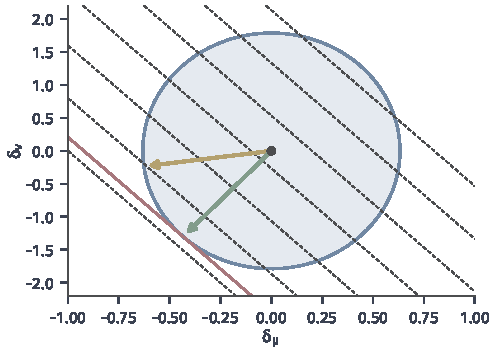
\includegraphics[width=84mm]{figures/07-probability/07-distribution-optimization/matplotlib/igeo-steepest-descent/figure.pdf}
  \caption{$\mathcal{N}(1,4)$处问题~\eqref{eq:igeo-steepest-problem}的几何，坐标为位移$(\delta_{\mu},\delta_{v})$。蓝色椭圆为$\frac12\bm{\delta}^{\top}\bm{G}\bm{\delta}=0.05$，深灰虚线为一阶变化$\langle\bm{g},\bm{\delta}\rangle$的等值线，红线是与椭圆相切的最低等值线。绿色箭头为自然梯度步，黄色箭头为缩放到同一椭圆上的负梯度。}
  \label{fig:igeo-steepest-descent}
\end{BookInlineFigure}

图~\ref{fig:igeo-steepest-descent}把问题~\eqref{eq:igeo-steepest-problem}画了出来。目标的一阶变化在位移平面上是一族平行直线，可行集是Fisher椭圆。最优点是椭圆与最低一条等值线的切点，它在绿色箭头的末端；黄色箭头末端所在的等值线高出不少。这里两个方向的一阶下降比约为$0.78$，差距来自椭圆的扁平程度：在$\bm{G}$各向同性的点，两个方向重合。

把预算想成固定大小的步伐，问题~\eqref{eq:igeo-steepest-problem}就是一种信赖域子问题：在可信的范围内用线性模型选方向，只是范围由分布的变化而不是参数的欧氏距离来划定，可参考\BookChapterRef{chap:trust-region}{卷五第9章“信赖域”}。若$\Pi$本身在候选族内，在最优点$\bm{\theta}^{*}$附近，$D_{\mathrm{KL}}(Q_{\bm{\theta}}\Vert\Pi)$恰好就是$Q_{\bm{\theta}}$与$Q_{\bm{\theta}^{*}}$之间的KL散度，它的Hessian在$\bm{\theta}^{*}$处等于$\bm{G}(\bm{\theta}^{*})$；这时自然梯度在最优点附近与Newton方向几乎一致。

\paragraph{信息矩阵退化时}
定理~\ref{thm:igeo-steepest}要求$\bm{G}$正定。$\bm{G}$奇异时，不能直接写$\bm{G}^{-1}$，而要先回到第~\ref{sec:igeo-fisher}节，辨认退化来自参数冗余还是一阶失效，在有效的坐标上重新建立问题。

先看参数冗余。在$\mathcal{N}(a+b,1)$中逼近$\Pi=\mathcal{N}(1,1)$，记$c=a+b$，目标是$L=\frac12(c-1)^{2}$。梯度与信息矩阵分别是
\[
  \bm{g}=(c-1)\begin{bmatrix}1\\1\end{bmatrix},\qquad\bm{G}=\begin{bmatrix}1&1\\1&1\end{bmatrix}.
\]
$\bm{G}$的零空间沿$(1,-1)$，沿这个方向分布不变，目标也不变，所以$\bm{g}$自动与它正交。去掉冗余，直接用$c$作参数，$G_{cc}=1$，自然梯度是$c-1$。若坚持在$(a,b)$中计算，可以用Moore--Penrose伪逆，$\bm{G}^{\dagger}\bm{g}=\frac{c-1}{2}(1,1)$，它在$c$上引起的变化同样是$c-1$；伪逆只是从无穷多个等价的位移中选了欧氏长度最短的那一个，零空间方向上走多少是任意约定。

再看一阶失效。在$\mathcal{N}(\theta^{3},1)$中逼近同一个$\Pi$，目标是$L=\frac12(\theta^{3}-1)^{2}$，
\[
  g(\theta)=3\theta^{2}(\theta^{3}-1),\qquad G(\theta)=9\theta^{4},\qquad\frac{g(\theta)}{G(\theta)}=\frac{\theta^{3}-1}{3\theta^{2}} .
\]
在$\theta=0$处普通梯度为零，$\theta=0$是$L$的驻点，可分布$\mathcal{N}(0,1)$离最优的$\mathcal{N}(1,1)$还很远；自然梯度则在$\theta\to0$时趋于无穷。两者都是坐标的毛病：用均值$m=\theta^{3}$作参数，$G_{mm}=1$，自然梯度是$m-1$，在$m=0$附近完全正常。

\begin{BookInlineFigure}
  \centering
  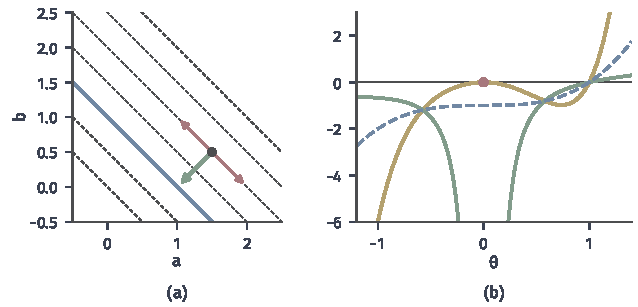
\includegraphics[width=108mm]{figures/07-probability/07-distribution-optimization/matplotlib/igeo-degenerate/figure.pdf}
  \caption{信息矩阵退化的两种情形。(a)$\mathcal{N}(a+b,1)$逼近$\mathcal{N}(1,1)$：深灰虚线是$a+b$为常数的直线，其上分布相同，蓝线$a+b=1$是全部最优参数；在$(1.5,0.5)$处，红色双箭头为$\bm{G}$的零空间方向，绿色箭头为伪逆给出的下降位移。(b)$\mathcal{N}(\theta^{3},1)$逼近$\mathcal{N}(1,1)$：黄线为普通梯度$3\theta^{2}(\theta^{3}-1)$，在红点$\theta=0$处为零；绿线为$g/G=(\theta^{3}-1)/(3\theta^{2})$，在$0$附近发散；蓝色虚线为均值坐标下的自然梯度$m-1$，按$m=\theta^{3}$画在$\theta$轴上。}
  \label{fig:igeo-degenerate}
\end{BookInlineFigure}

图~\ref{fig:igeo-degenerate}对照了这两种情形。实践中常用的另一个办法是把$\bm{G}$换成$\bm{G}+\gamma\bm{I}$，$\gamma>0$，矩阵总是可逆。它能防止数值上的崩溃，却没有回答问题：(b)中$\theta$接近$0$时，加上$\gamma$以后的方向主要由$\gamma$的大小决定，而不是由分布的变化决定。先识别退化方向，再在有效坐标上建立问题，加正则项只作为数值上的保护。

\subsection{重参数化后的更新}
\label{sec:igeo-reparam-update}

普通梯度依赖坐标，这一点从变换公式就能看出。设$\bm{\theta}=\bm{\varphi}(\bm{\xi})$，Jacobian为$\bm{J}$，由链式法则，同一个目标函数在两套坐标中的梯度满足
\[
  \bm{g}_{\bm{\xi}}=\bm{J}^{\top}\bm{g}_{\bm{\theta}} .
\]
在$\bm{\xi}$坐标中沿$-\bm{g}_{\bm{\xi}}$走一小步，换算到$\bm{\theta}$坐标，位移是
\[
  -\bm{J}\bm{g}_{\bm{\xi}}=-\bm{J}\bm{J}^{\top}\bm{g}_{\bm{\theta}} .
\]
除非$\bm{J}\bm{J}^{\top}=\bm{I}$，它与在$\bm{\theta}$坐标中沿$-\bm{g}_{\bm{\theta}}$走的位移不同：两种坐标下的“梯度下降”是两个不同的方向。

自然梯度没有这个问题。由式~\eqref{eq:igeo-reparam}，$\bm{G}^{\Xi}=\bm{J}^{\top}\bm{G}\bm{J}$，于是
\begin{equation}
  \bm{J}\,(\bm{G}^{\Xi})^{-1}\bm{g}_{\bm{\xi}}=\bm{J}\,\bm{J}^{-1}\bm{G}^{-1}\bm{J}^{-\top}\bm{J}^{\top}\bm{g}_{\bm{\theta}}=\bm{G}^{-1}\bm{g}_{\bm{\theta}} .
  \label{eq:igeo-natural-invariance}
\end{equation}
$\bm{\xi}$坐标中的自然梯度换算到$\bm{\theta}$坐标，恰好是$\bm{\theta}$坐标中的自然梯度，两者是同一个切向量。同样，
\[
  \bm{g}_{\bm{\xi}}^{\top}(\bm{G}^{\Xi})^{-1}\bm{g}_{\bm{\xi}}=\bm{g}_{\bm{\theta}}^{\top}\bm{G}^{-1}\bm{g}_{\bm{\theta}},
\]
自然梯度在Fisher度量下的长度也与坐标无关。这与定理~\ref{thm:igeo-steepest}一致：问题~\eqref{eq:igeo-steepest-problem}的目标与约束都只依赖分布，答案自然不依赖于怎样给分布编号。

\paragraph{例中的核对}
把例子改写到自然参数。两套坐标之间的变换是
\[
  (\theta_1,\theta_2)=\Bigl(\frac{\mu}{v},\,-\frac{1}{2v}\Bigr),\qquad(\mu,v)=\Bigl(-\frac{\theta_1}{2\theta_2},\,-\frac{1}{2\theta_2}\Bigr),
\]
起点$\mathcal{N}(1,4)$对应$\bm{\theta}=(0.25,\,-0.125)$。后一个变换的Jacobian在起点处为
\[
  \bm{J}=\frac{\partial(\mu,v)}{\partial(\theta_1,\theta_2)}=\begin{bmatrix}-\frac{1}{2\theta_2}&\frac{\theta_1}{2\theta_2^{2}}\\0&\frac{1}{2\theta_2^{2}}\end{bmatrix}=\begin{bmatrix}4&8\\0&32\end{bmatrix}.
\]
这里$\bm{\theta}$扮演新坐标$\bm{\xi}$的角色。由$\bm{g}_{\bm{\theta}}=\bm{J}^{\top}\bm{g}_{\mu,v}$，
\[
  \bm{g}_{\bm{\theta}}=\begin{bmatrix}4&0\\8&32\end{bmatrix}\begin{bmatrix}1\\0.375\end{bmatrix}=\begin{bmatrix}4\\20\end{bmatrix}.
\]

由式~\eqref{eq:igeo-reparam}算出的信息矩阵是
\[
  \bm{J}^{\top}\begin{bmatrix}\frac14&0\\0&\frac1{32}\end{bmatrix}\bm{J}=\begin{bmatrix}4&8\\8&48\end{bmatrix},
\]
正是第~\ref{sec:igeo-exponential}节由式~\eqref{eq:igeo-gauss-natural-fisher}得到的矩阵。解$\bm{G}\bm{d}=\bm{g}_{\bm{\theta}}$得$\bm{d}=(0.25,\,0.375)$，换算回去，
\[
  \bm{J}\bm{d}=\begin{bmatrix}4\cdot0.25+8\cdot0.375\\32\cdot0.375\end{bmatrix}=\begin{bmatrix}4\\12\end{bmatrix},
\]
正是$(\mu,v)$坐标中的自然梯度，并且$\bm{g}_{\bm{\theta}}^{\top}\bm{d}=1+7.5=8.5$与前面相同。

普通梯度则不然：自然参数中的负梯度$-(4,20)$换算到$(\mu,v)$坐标，是
\[
  -\bm{J}\begin{bmatrix}4\\20\end{bmatrix}=-\begin{bmatrix}176\\640\end{bmatrix},
\]
与$(\mu,v)$坐标中的负梯度$-(1,\ 0.375)$方向不同。

\paragraph{有限步的差别}
自然梯度给出的是切方向，实际更新还要走一个有限步。最简单的规则是在当前坐标中直接相加：$\bm{\theta}\leftarrow\bm{\theta}-\alpha\,\bm{G}^{-1}\bm{g}$。三套坐标下的方向在起点相切，但各自是“直线”的那条曲线并不相同，走出有限距离后到达的分布也不同。

取$\alpha=\frac18$，从$\mathcal{N}(1,4)$出发，在三套坐标中各走一步。在$(\mu,v)$坐标中，自然梯度为$(4,12)$，
\[
  (\mu,v)\leftarrow(1-\tfrac12,\ 4-\tfrac32)=(0.5,\ 2.5).
\]
在自然参数中，自然梯度为$(0.25,0.375)$，
\[
  \bm{\theta}\leftarrow(0.25,\,-0.125)-\tfrac18(0.25,\,0.375)=(0.21875,\,-0.171875),
\]
换回$(\mu,v)\approx(0.636,\ 2.909)$。在$(\mu,\tau)$坐标中，$\tau=\ln v$，信息矩阵为$\operatorname{diag}(1/v,\,\frac12)$，梯度为$(\mu,\ v\,\partial L/\partial v)=(1,\ 1.5)$，自然梯度为$(4,\ 3)$，
\[
  (\mu,\tau)\leftarrow(1-\tfrac12,\ \ln4-\tfrac38),\qquad v=4\mathrm{e}^{-3/8}\approx2.749 .
\]
三个新分布的目标值分别是$0.417$、$0.623$与$0.494$。

另一方面，令步长趋于零，自然梯度更新的连续极限是常微分方程
\begin{equation}
  \dot{\bm{\theta}}(t)=-\bm{G}\bigl(\bm{\theta}(t)\bigr)^{-1}\nabla L\bigl(\bm{\theta}(t)\bigr),
  \label{eq:igeo-natural-flow}
\end{equation}
它的解曲线称为\term{自然梯度流}（natural gradient flow）。由式~\eqref{eq:igeo-natural-invariance}与链式法则，一套坐标中的解换算到另一套坐标，仍满足那里的方程~\eqref{eq:igeo-natural-flow}，所以各坐标给出同一条分布曲线。

在本例的自然参数中，下一节会看到自然梯度恰为$\bm{\theta}-\bm{\theta}_{\Pi}$，其中$\bm{\theta}_{\Pi}=(0,-\frac12)$是目标的自然参数。于是流的解是
\[
  \bm{\theta}(t)=\bm{\theta}_{\Pi}+\mathrm{e}^{-t}\bigl(\bm{\theta}(0)-\bm{\theta}_{\Pi}\bigr).
\]
换到$(\mu,v)$平面，它是线段$v=1+3\mu$。

\begin{BookInlineFigure}
  \centering
  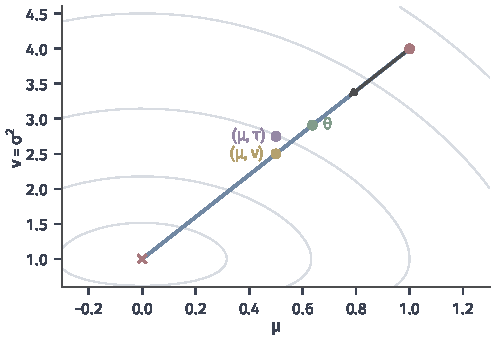
\includegraphics[width=84mm]{figures/07-probability/07-distribution-optimization/matplotlib/igeo-finite-steps/figure.pdf}
  \caption{从$\mathcal{N}(1,4)$（红点）出发、步长$\alpha=\frac18$的一步自然梯度更新，画在$(\mu,v)$平面上，目标为$\mathcal{N}(0,1)$（红叉）。蓝线是自然梯度流，深灰箭头是三套坐标共同的切方向。黄、绿、紫三点分别是在$(\mu,v)$、自然参数$\theta$、$(\mu,\tau)$坐标中直接相加得到的新分布。浅灰线为$L$的等值线。}
  \label{fig:igeo-finite-steps}
\end{BookInlineFigure}

图~\ref{fig:igeo-finite-steps}中，$(\mu,v)$与自然参数两步恰好落在流的直线上，只是走得远近不同；$(\mu,\tau)$一步偏离了这条线。三者一阶相同，二阶以上的差别来自“在坐标中走直线”这一规则本身。若要求有限步也与坐标无关，需要规定从切向量回到参数空间的方式，例如沿Fisher度量的测地线走，或者采用某种满足一阶条件的回缩，这正是流形上的迭代要处理的问题。实际中，这种依赖性通过选择合适的坐标和足够小的步长来控制，并由目标值与参数可行性来检查。


\section{族内更新的实施}
\label{sec:igeo-implementation}

把自然梯度用到第~\ref{chap:distribution-approximation}章的逼近目标上，每一步要做四件事：算出目标的梯度，得到Fisher信息或它与向量的乘积，解一个线性方程得到方向，再定步长并保证新参数仍然合法。前两件常常只能近似完成，后两件则决定了算法在有限步时的表现。

\paragraph{主要思想}
由定义~\ref{def:igeo-natural-gradient}，方向$\bm{d}=\bm{G}^{-1}\bm{g}$。实际计算从不形成逆矩阵，而是解线性方程。为了在$\bm{G}$接近奇异时仍能求解，可以加上一个小的非负数$\gamma$，于是第$t$轮的方向与更新为
\begin{equation}
  \bigl(\bm{G}(\bm{\theta}^{(t)})+\gamma\bm{I}\bigr)\bm{d}^{(t)}=\nabla L(\bm{\theta}^{(t)}),\qquad
  \bm{\theta}^{(t+1)}=\bm{\theta}^{(t)}-\alpha_{t}\,\bm{d}^{(t)}.
  \label{eq:igeo-ngd-update}
\end{equation}
$\gamma=0$时这就是自然梯度步。$\gamma>0$时，$-\bm{d}^{(t)}$是二次模型
\[
  \langle\bm{g},\bm{\delta}\rangle+\frac12\bm{\delta}^{\top}(\bm{G}+\gamma\bm{I})\bm{\delta}
\]
的最小点，相当于在Fisher二次型之外再对参数的欧氏长度加一点惩罚；上一节已经说明，它只是数值上的保护，不能代替对退化方向的分析。

梯度从哪里来，取决于目标的形式。以
\[
  L(\bm{\theta})=D_{\mathrm{KL}}(Q_{\bm{\theta}}\Vert\Pi)=\int q_{\bm{\theta}}\ln\frac{q_{\bm{\theta}}}{\pi}\,\mathrm{d}\nu
\]
为例，$q_{\bm{\theta}}$与$\pi$是相对$\nu$的密度。在积分号下求导需要的条件由第~\ref{chap:expectation-gradient-estimation}章讨论；条件满足时，对被积函数$q_{\bm{\theta}}\ln q_{\bm{\theta}}-q_{\bm{\theta}}\ln\pi$求导，再利用“密度的梯度等于密度乘以得分”与式~\eqref{eq:igeo-score-mean}，得到
\[
  \begin{aligned}
    \nabla L(\bm{\theta})&=\int\nabla q_{\bm{\theta}}\ln\frac{q_{\bm{\theta}}}{\pi}\,\mathrm{d}\nu+\int\nabla q_{\bm{\theta}}\,\mathrm{d}\nu\\
    &=\mathbb{E}_{\bm{\theta}}\Bigl[\bm{s}_{\bm{\theta}}(X)\ln\frac{q_{\bm{\theta}}(X)}{\pi(X)}\Bigr].
  \end{aligned}
\]

在指数族中，由式~\eqref{eq:igeo-expfam-score}，这是$\operatorname{Cov}_{\bm{\theta}}(\bm{T},\ln q_{\bm{\theta}}-\ln\pi)$。若$\Pi$也属于这个族，自然参数为$\bm{\theta}_{\Pi}$，则
\[
  \ln q_{\bm{\theta}}-\ln\pi=\langle\bm{\theta}-\bm{\theta}_{\Pi},\bm{T}\rangle+\text{常数},
\]
于是梯度与自然梯度分别是
\[
  \nabla L(\bm{\theta})=\bm{G}(\bm{\theta})(\bm{\theta}-\bm{\theta}_{\Pi}),\qquad\bm{G}(\bm{\theta})^{-1}\nabla L(\bm{\theta})=\bm{\theta}-\bm{\theta}_{\Pi}.
\]

指数族的自然参数中还有一个省去解方程的办法。目标若写成均值参数的函数，由链式法则与$\partial\bm{m}/\partial\bm{\theta}=\bm{G}$，
\[
  \nabla_{\bm{\theta}}L=\bm{G}(\bm{\theta})\,\nabla_{\bm{m}}L,\qquad\text{从而}\qquad\bm{G}(\bm{\theta})^{-1}\nabla_{\bm{\theta}}L=\nabla_{\bm{m}}L .
\]
在自然参数上走自然梯度步，等于用均值坐标中的普通梯度去更新自然参数。均值坐标下的目标容易求导时，这一形式最省事。

步长分两层控制。第一层是局部预算：由定理~\ref{thm:igeo-steepest}，步长$\alpha$对应的局部KL约为$\frac12\alpha^{2}\,\bm{g}^{\top}\bm{d}$，要它不超过$\varepsilon$，取
\[
  \alpha\leq\sqrt{2\varepsilon/(\bm{g}^{\top}\bm{d})} .
\]
第二层是实际检查：新参数必须属于$\Theta$（例如高斯族的自然参数要求$\theta_2<0$），并且目标要有足够的下降，例如Armijo条件
\begin{equation}
  L(\bm{\theta}-\alpha\bm{d})\leq L(\bm{\theta})-c\,\alpha\,\bm{g}^{\top}\bm{d},\qquad0<c<1 ;
  \label{eq:igeo-armijo}
\end{equation}
不满足就把$\alpha$减半重试，这种回溯可参考\BookChapterRef{chap:smooth-optimization}{卷五第5章“光滑优化基础”}。量$\bm{g}^{\top}\bm{d}$等于$\bm{g}^{\top}\bm{G}^{-1}\bm{g}$，它是自然梯度在Fisher度量下长度的平方，由上一节，它与坐标无关，适合作为停止判据。

\paragraph{计算过程}
下面沿用上一节的例子：目标$\Pi=\mathcal{N}(0,1)$，候选为高斯族，目标函数为式~\eqref{eq:igeo-running-objective}，在自然参数中计算，梯度与信息矩阵都用精确公式。取$\gamma=0$，试探步长$\alpha=\frac12$，Armijo常数$c=10^{-4}$，停止阈值$\mathrm{tol}=10^{-3}$。目标的自然参数是$\bm{\theta}_{\Pi}=(0,\,-0.5)$。

\needspace{6\baselineskip}
\paragraph{变量}
\begin{itemize}
  \item $\bm{\theta}\in\mathbb{R}^{k}$：当前参数，例中$k=2$，并随时换算出$(\mu,v)$。
  \item $\bm{g}\in\mathbb{R}^{k}$：当前梯度$\nabla L(\bm{\theta})$。
  \item $\bm{G}\in\mathbb{R}^{k\times k}$：当前Fisher信息，例中由式~\eqref{eq:igeo-gauss-natural-fisher}计算。
  \item $\bm{C}\in\mathbb{R}^{k\times k}$：$\bm{G}+\gamma\bm{I}$的Cholesky因子，下三角，用后即弃。
  \item $\bm{d}\in\mathbb{R}^{k}$：方向，解方程~\eqref{eq:igeo-ngd-update}得到。
  \item $\alpha$：本轮步长；$L$：当前目标值；$t$：轮次。
\end{itemize}

\paragraph{初始化}
取起点$\bm{\theta}^{(0)}$并检查它属于$\Theta$，算出$L(\bm{\theta}^{(0)})$，令$t=0$。例中起点为$\mathcal{N}(1,4)$，
\[
  \bm{\theta}^{(0)}=(0.25,\ -0.125),\qquad L^{(0)}=-\ln2+2\approx1.3069 .
\]

\needspace{6\baselineskip}
\paragraph{每轮更新}
在第$t$轮：
\begin{enumerate}
  \item \textbf{求梯度与信息矩阵。}计算$\bm{g}=\nabla L(\bm{\theta}^{(t)})$与$\bm{G}=\bm{G}(\bm{\theta}^{(t)})$。例中第一轮$(\mu,v)=(1,4)$，由式~\eqref{eq:igeo-gauss-natural-fisher}与$\bm{g}=\bm{G}(\bm{\theta}-\bm{\theta}_{\Pi})$，
  \[
    \bm{G}=\begin{bmatrix}4&8\\8&48\end{bmatrix},\qquad\bm{g}=\begin{bmatrix}4&8\\8&48\end{bmatrix}\begin{bmatrix}0.25\\0.375\end{bmatrix}=\begin{bmatrix}4\\20\end{bmatrix}.
  \]

  \item \textbf{解方向。}对$\bm{G}+\gamma\bm{I}$作Cholesky分解$\bm{C}\bm{C}^{\top}$，先解$\bm{C}\bm{y}=\bm{g}$，再解$\bm{C}^{\top}\bm{d}=\bm{y}$；分解失败说明矩阵不是正定的，应回到退化分析，而不是继续。例中第一轮
  \[
    \bm{C}=\begin{bmatrix}2&0\\4&4\sqrt2\end{bmatrix}.
  \]
  前代给出
  \[
    y_1=\frac42=2,\qquad y_2=\frac{20-4\cdot2}{4\sqrt2}=\frac{3}{\sqrt2},
  \]
  回代给出
  \[
    d_2=\frac{y_2}{4\sqrt2}=\frac38,\qquad d_1=\frac{2-4\cdot\frac38}{2}=\frac14,
  \]
  即$\bm{d}=(0.25,\,0.375)$。于是$\bm{g}^{\top}\bm{d}=1+7.5=8.5$。

  \item \textbf{检查停止。}若$\bm{g}^{\top}\bm{d}\leq\mathrm{tol}$，输出$\bm{\theta}^{(t)}$并结束。例中第一轮$8.5>10^{-3}$，继续。

  \item \textbf{试探步长。}令$\bm{\theta}'=\bm{\theta}^{(t)}-\alpha\bm{d}$。若$\bm{\theta}'\notin\Theta$，或式~\eqref{eq:igeo-armijo}不成立，把$\alpha$减半重试；成立则接受$\bm{\theta}^{(t+1)}=\bm{\theta}'$，令$t\leftarrow t+1$。例中第一轮
  \[
    \bm{\theta}'=(0.25,\,-0.125)-\tfrac12(0.25,\,0.375)=(0.125,\ -0.3125),
  \]
  $\theta'_2<0$，可行；换算得$v=1/(2\cdot0.3125)=1.6$，$\mu=0.125\cdot1.6=0.2$，由式~\eqref{eq:igeo-running-objective}，
  \[
    L(\bm{\theta}')=-\tfrac12\ln1.6+\tfrac{1.6+0.04}{2}-\tfrac12\approx0.0850 ,
  \]
  远小于Armijo的界$1.3069-10^{-4}\cdot\frac12\cdot8.5$，接受。
\end{enumerate}

例中第二轮从$\mathcal{N}(0.2,\,1.6)$出发。由式~\eqref{eq:igeo-gauss-natural-fisher}，
\[
  \bm{G}=\begin{bmatrix}1.6&0.64\\0.64&5.376\end{bmatrix},\qquad\bm{\theta}-\bm{\theta}_{\Pi}=\begin{bmatrix}0.125\\0.1875\end{bmatrix},\qquad\bm{g}=\begin{bmatrix}0.32\\1.088\end{bmatrix}.
\]
Cholesky因子与解出的方向是
\[
  \bm{C}\approx\begin{bmatrix}1.265&0\\0.506&2.263\end{bmatrix},\qquad\bm{d}=\begin{bmatrix}0.125\\0.1875\end{bmatrix},
\]
其中$C_{2,2}=\sqrt{5.376-0.506^{2}}\approx2.263$。于是
\[
  \bm{g}^{\top}\bm{d}=0.04+0.204=0.244 .
\]
它仍大于阈值。试探步为
\[
  \bm{\theta}'=(0.125,\,-0.3125)-\tfrac12(0.125,\,0.1875)=(0.0625,\ -0.40625),
\]
可行，对应$\mathcal{N}(\frac1{13},\frac{16}{13})$，目标值约$0.0145$，满足式~\eqref{eq:igeo-armijo}，接受。

此后每一轮都重复同样的计算。表~\ref{tab:igeo-ngd-rounds}列出各轮的结果。每轮的$\bm{d}$都等于$\bm{\theta}-\bm{\theta}_{\Pi}$，于是
\[
  \bm{\theta}^{(t)}-\bm{\theta}_{\Pi}=2^{-t}\bigl(\bm{\theta}^{(0)}-\bm{\theta}_{\Pi}\bigr).
\]
第$5$轮开始时$\bm{g}^{\top}\bm{d}\approx3.5\times10^{-4}$，已低于阈值$10^{-3}$，算法停止。最终得到
\[
  \bm{\theta}^{(5)}=\Bigl(\frac1{128},\,-\frac{125}{256}\Bigr),
\]
即$\mathcal{N}(0.008,\,1.024)$，目标值约$1.7\times10^{-4}$。

\begin{BookInlineTable}
  \centering
  \caption{自然梯度迭代的各轮结果，$\alpha=\frac12$，起点$\mathcal{N}(1,4)$，目标$\mathcal{N}(0,1)$。$\bm{g}^{\top}\bm{d}$是本轮开始时自然梯度长度的平方，用于停止判据。}
  \label{tab:igeo-ngd-rounds}
  \begin{tabular}{rrrrr}
    \toprule
    $t$ & $\mu$ & $v$ & $L$ & $\bm{g}^{\top}\bm{d}$ \\
    \midrule
    0 & 1 & 4 & 1.3069 & 8.5 \\
    1 & 0.2 & 1.6 & 0.0850 & 0.244 \\
    2 & 0.0769 & 1.2308 & 0.0145 & 0.0339 \\
    3 & 0.0345 & 1.1034 & 0.00310 & 0.00666 \\
    4 & 0.0164 & 1.0492 & 0.00072 & 0.00149 \\
    5 & 0.0080 & 1.0240 & 0.00017 & 0.00035 \\
    \bottomrule
  \end{tabular}
\end{BookInlineTable}

在这个例子里，若取$\alpha=1$，第一步就直接到达$\bm{\theta}_{\Pi}$。这是因为目标在族内、族是指数族、又在自然参数中计算，三者同时成立时自然梯度恰为$\bm{\theta}-\bm{\theta}_{\Pi}$；一般的逼近问题没有这样的巧合。

\paragraph{算法分析}
先与普通梯度比较。同一个问题在自然参数中用普通梯度，起点处$\bm{g}=(4,20)$，若也取$\alpha=\frac12$，第一步落到$\bm{\theta}=(-1.75,\,-10.125)$，方差约$0.049$，远远越过目标。要避免这种越过，步长要小到约$0.02$；此后在最优点附近，目标的Hessian等于那里的信息矩阵$\operatorname{diag}(1,2)$，每步只把误差缩小约$2\%$。在$(\mu,v)$坐标中用普通梯度、$\alpha=\frac12$，则可以稳定收敛，只是前期较慢。图~\ref{fig:igeo-ngd-runs}对照了三者：普通梯度的表现取决于选哪套坐标，自然梯度的方向则不依赖于这一选择。

\begin{BookInlineFigure}
  \centering
  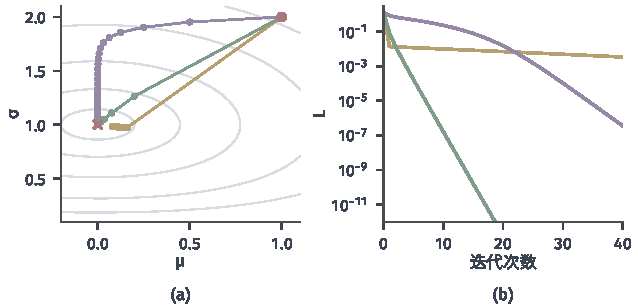
\includegraphics[width=108mm]{figures/07-probability/07-distribution-optimization/matplotlib/igeo-ngd-runs/figure.pdf}
  \caption{从$\mathcal{N}(1,4)$（红点）逼近$\mathcal{N}(0,1)$（红叉），目标$D_{\mathrm{KL}}(Q\Vert\Pi)$，各迭代$40$轮。绿：自然梯度，$\alpha=\frac12$；黄：自然参数中的普通梯度，$\alpha=0.02$；紫：$(\mu,v)$坐标中的普通梯度，$\alpha=\frac12$。(a)迭代点画在$(\mu,\sigma)$平面上，浅灰线为目标的等值线；(b)目标值随迭代次数的变化，纵轴为对数刻度。}
  \label{fig:igeo-ngd-runs}
\end{BookInlineFigure}

收敛方面，表~\ref{tab:igeo-ngd-rounds}的线性收敛是例子的特殊结构给出的。一般情形下，若$L$在非退化的最小点$\bm{\theta}^{*}$附近二阶光滑、$\bm{G}$正定且连续，步长适当时迭代在$\bm{\theta}^{*}$附近线性收敛，速率由$\bm{G}(\bm{\theta}^{*})^{-1}\nabla^{2}L(\bm{\theta}^{*})$的特征值决定；当这个矩阵接近单位阵时，例如目标在族内且用$D_{\mathrm{KL}}(Q\Vert\Pi)$，取$\alpha$接近$1$可以接近Newton法的速度。这只是局部的结论：离最优点很远时，Fisher度量对$L$的曲率没有任何保证，仍要靠回溯和可行性检查。

信息矩阵常常只能估计。由式~\eqref{eq:igeo-fisher}，可以从当前候选分布$Q_{\bm{\theta}}$抽取$n$个独立样本$X_1,\dots,X_n$，用
\begin{equation}
  \widehat{\bm{G}}=\frac1n\sum_{i=1}^{n}\bm{s}_{\bm{\theta}}(X_i)\bm{s}_{\bm{\theta}}(X_i)^{\top}
  \label{eq:igeo-fisher-estimate}
\end{equation}
代替。样本必须来自$Q_{\bm{\theta}}$本身：若改用目标分布的样本计算$\bm{s}_{\bm{\theta}}\bm{s}_{\bm{\theta}}^{\top}$的平均，得到的是得分外积在$\Pi$下的期望，常称为\term{经验Fisher矩阵}（empirical Fisher matrix），除非$Q_{\bm{\theta}}=\Pi$，它不等于$\bm{G}(\bm{\theta})$，所得方向也不再是自然梯度。估计误差按Monte Carlo的速率$n^{-1/2}$缩小，误差分析与方差控制分别见第~\ref{chap:monte-carlo-integration-error}章和第~\ref{chap:variance-reduction}章，梯度本身的随机估计见第~\ref{chap:expectation-gradient-estimation}章。

图~\ref{fig:igeo-fisher-estimate}在例子的起点$\mathcal{N}(1,4)$处做了这一估计。梯度取精确值，$\widehat{\bm{G}}$由$n$个样本得到，方向误差以Fisher范数相对计量。$n=20$时相对误差超过$1$，方向几乎不可信；$n=2000$时约为$8\%$。样本少时，$\widehat{\bm{G}}$的小特征值估计不稳，加上$\gamma$可以避免方向被放大到不合理的长度。

\begin{BookInlineFigure}
  \centering
  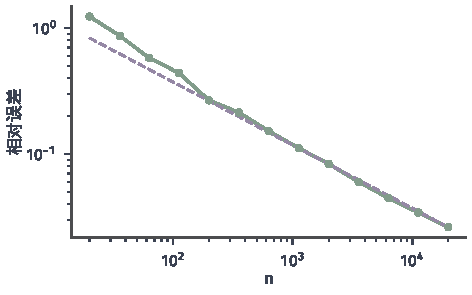
\includegraphics[width=80mm]{figures/07-probability/07-distribution-optimization/matplotlib/igeo-fisher-estimate/figure.pdf}
  \caption{在$\mathcal{N}(1,4)$处用$n$个样本估计自然参数坐标下的Fisher信息，所得方向$\widehat{\bm{d}}=\widehat{\bm{G}}^{-1}\bm{g}$的相对误差$\lVert\widehat{\bm{d}}-\bm{d}\rVert_{\bm{G}}/\lVert\bm{d}\rVert_{\bm{G}}$。绿：$500$次重复的均方根，随机种子$728$；紫色虚线：参考斜率$n^{-1/2}$，在$n=20000$处与绿线对齐。}
  \label{fig:igeo-fisher-estimate}
\end{BookInlineFigure}

计算量方面，用$n$个样本形成$\widehat{\bm{G}}$需要$O(nk^{2})$次运算，Cholesky分解需要$O(k^{3})$，可参考\BookChapterRef{chap:direct-linear-solvers}{卷二第12章“线性方程的直接求解”}。参数维数$k$很大时，两者都负担不起。注意到方程只需要矩阵与向量的乘积，而
\[
  \bm{G}\bm{u}=\mathbb{E}_{\bm{\theta}}\bigl[\bm{s}_{\bm{\theta}}(X)\,\langle\bm{s}_{\bm{\theta}}(X),\bm{u}\rangle\bigr]
\]
可以用同一批样本以$O(nk)$的代价得到，于是可以用共轭梯度法只通过这种\term{Fisher向量积}（Fisher-vector product）近似求解，不必形成$\bm{G}$，可参考\BookChapterRef{chap:krylov-methods}{卷二第15章“Krylov子空间法”}。共轭梯度迭代几步就停止，得到的是近似方向；也可以把$\bm{G}$近似为对角或分块对角矩阵。这些近似都改变了方向，需要用目标值的实际下降来检验。

最后，式~\eqref{eq:igeo-ngd-update}的“在坐标中相加”只是从切向量回到参数空间的一种规则。上一节已经看到，换一套坐标，有限步会到达不同的分布；而参数域的边界，例如方差必须为正，也要单独处理。改用无约束的坐标（如$\tau=\ln v$）、沿测地线移动、或采用满足一阶条件的回缩，都是可选的办法。Fisher度量下的Riemann梯度正是自然梯度，流形上的回缩、向量传输与收敛分析可参考\BookChapterRef{chap:manifold-optimization}{卷五第25章“流形优化”}。

局部几何给出的是方向与尺度，它不代替其他三项检验：迭代是否在全局上收敛，要看目标本身的性质；信息矩阵估计得是否足够准确，要看样本数与方差；族内最优的分布离目标还有多远，是第~\ref{chap:distribution-approximation}章逼近误差的问题，选择更好的更新方向并不能缩小这一差距。


\section{本章小结}
\label{sec:igeo-summary}

章首的问题是：高斯族中同样的参数位移为什么引起大小悬殊的分布变化，这种变化用什么度量，又怎样用于参数更新。本章的回答是一条链：得分描述密度在各处怎样相对变化，Fisher信息把这些变化汇总成参数位移的二次型，邻近分布间的KL散度在二阶意义下正是这个二次型的一半，自然梯度再用这把尺子选取族内更新的方向。图~\ref{fig:igeo-chain-map}标出了链上每一步所需的条件。

\begin{BookInlineFigure}
  \centering
  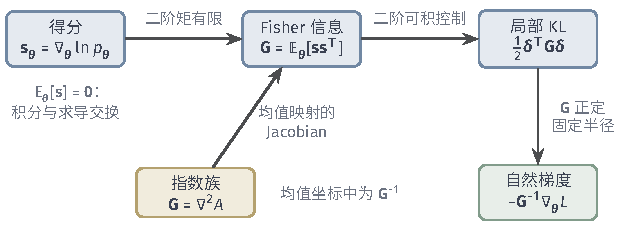
\includegraphics[width=106mm]{figures/07-probability/07-distribution-optimization/tikz/igeo-chain-map/figure.pdf}
  \caption{本章的主线与各步条件。蓝框依次为得分、Fisher信息与局部KL，箭头旁是由前一项得到后一项所需的条件；绿框为自然梯度，需要$\bm{G}$正定；黄框为指数族，其中Fisher信息是对数配分函数的Hessian，也是均值映射的Jacobian。}
  \label{fig:igeo-chain-map}
\end{BookInlineFigure}

正则分布族是这条链的起点：参数集合是开集，支撑不随参数移动，密度对参数可微，并且求导能与积分交换。在这些条件下，得分的期望为零，这是总质量守恒的表现；支撑随参数移动的模型（如$\operatorname{Unif}(0,\theta)$）会多出边界项，KL散度甚至可能为无穷，本章的结论不适用于它们。Fisher信息总是半正定的，但不一定正定。参数冗余、某点的一阶退化与整体不可辨识是三件不同的事，凡要求逆，都要先排除前两种情形。

KL散度的二阶展开说明Fisher信息就是分布变化的局部尺度，系数$\frac12$对应自然对数。它只在一点附近成立：位移稍大，两个方向的KL散度就明显分开，也可能因为整体不可辨识而降到零。换参数坐标时，Fisher信息按$\bm{J}^{\top}\bm{G}\bm{J}$变换，切向量的二次型保持不变。表~\ref{tab:igeo-summary}汇总了高斯族在几套坐标下的结果。

\begin{BookInlineTable}
  \centering
  \caption{高斯族$\mathcal{N}(\mu,\sigma^{2})$在不同坐标下的Fisher信息，$v=\sigma^{2}$，$\tau=\ln v$。各行表示同一个分布族，局部变化的二次型相同。}
  \label{tab:igeo-summary}
  \begin{tabular}{lll}
    \toprule
    坐标 & Fisher信息 & 特点 \\
    \midrule
    $(\mu,\sigma)$ & $\operatorname{diag}(1/\sigma^{2},\,2/\sigma^{2})$ & 尺度随$\sigma$缩小而增大 \\
    $(\mu,v)$ & $\operatorname{diag}(1/v,\,1/(2v^{2}))$ & 方差方向随$v$增大变得便宜 \\
    $(\mu,\tau)$ & $\operatorname{diag}(1/v,\,1/2)$ & 方差方向的尺度处处相同 \\
    自然参数 & $\operatorname{Cov}(X,X^{2})$ & 非对角，等于$\nabla^{2}A$ \\
    均值参数 & 自然参数下信息的逆 & 与自然参数对偶 \\
    \bottomrule
  \end{tabular}
\end{BookInlineTable}

指数族把这些结构集中到对数配分函数上：得分是自然统计量减去均值，Fisher信息是$\nabla^{2}A$，KL散度是由$A$生成的Bregman距离。均值映射的Jacobian就是Fisher信息，所以均值坐标下的Fisher信息是它的逆；对偶势函数$A^{*}$在均值坐标中扮演$A$的角色。这些对应只在最小表示的正则指数族内部成立，冗余统计量与边界参数都会使它失效。

自然梯度是在固定的局部KL预算下使目标一阶下降最多的方向，要求Fisher信息正定、梯度非零。它在坐标变换下表示同一个切向量，普通梯度没有这个性质；但有限步更新还依赖步长和回到参数空间的规则，不同坐标中相加同一个方向，一般得到不同的新分布。实施时，方向由解线性方程得到，信息矩阵可能需要用候选分布自身的样本估计，大规模时只用Fisher向量积近似求解；步长要同时受局部预算、可行性与实际下降的约束。局部几何只回答“朝哪里走、一步走多远才算小”，全局收敛、估计精度与族内逼近误差都需要另外检验。

Fisher信息还出现在统计估计中：它给出由样本估计参数时精度的下界。那是在给定数据下讨论估计量的性质，属于统计推断的问题，可参考\BookChapterRef{chap:finite-sample-lower-bounds}{卷八第5章“有限样本的精度下界”}。


\chapter{最优运输}
\label{chap:optimal-transport}

直线上的三个位置$0,1,2$各有一份质量，分别是$0.5$、$0.3$、$0.2$；我们想把它们重新摆成$0.2$、$0.3$、$0.5$的样子。搬动一份质量的代价是质量乘以搬运距离的平方。怎样搬最省？两份质量表都是概率分布，每一种搬法都是一张行和、列和固定的非负表，也就是两个分布的一个耦合。第~\ref{chap:distribution-comparison}章用耦合的最小成本定义了Wasserstein距离，那里只需要这个最小值；本章把“怎样达到它”本身作为问题：给定两个边缘分布和一个成本，在全部耦合中找成本最低的那一个。

这个问题有三层。第一层是问题本身是否有解：耦合允许把一个点的质量拆开送往几处，要求“一个点只去一处”的运输映射则可能根本不存在；最低成本是否真被某个耦合取到，也要看成本和分布满足什么条件。第二层是怎样确认手里的方案已经最优：每个可行方案都给出最低成本的一个上界，对偶问题给出下界，两者相等时方案就被证实。第三层是怎样把它算出来：实数轴上的顺序、有限点上的线性规划、高斯分布的二次结构各自给出可计算的形式；一般的有限问题还可以加上熵正则化，用简单的交替缩放求近似解。

最后两节把最优耦合当作工具，构造新的分布。沿最优耦合把每份质量匀速推向目的地，得到连接两个分布的一条路径；对多个分布按权重求总运输成本最小的分布，得到它们的Wasserstein重心。这两种构造都移动质量的位置，与按权重混合两个分布完全不同。

本章回用第~\ref{chap:distribution-comparison}章的耦合、Wasserstein距离与有限支撑的Kantorovich--Rubinstein对偶，第~\ref{chap:weak-convergence-of-distributions}章的胎紧与弱收敛子列，第~\ref{chap:random-variables}章的分位数，以及线性规划的对偶理论。全章贯穿开头的三点例子。

\section{运输问题}
\label{sec:ot-problem}

先把章首的例子写成表。源位置$x=0,1,2$上的质量是
\[
 \bm{a}=(0.5,\ 0.3,\ 0.2),
\]
目标位置$y=0,1,2$上需要的质量是
\[
 \bm{b}=(0.2,\ 0.3,\ 0.5),
\]
把一份质量$m$从$x$搬到$y$的代价是$m\,(x-y)^{2}$，记成本矩阵$\bm{C}$，元素$c_{i,j}=(i-j)^{2}$（下标从$0$起）。一个搬运方案说清从每个$x_i$搬多少到每个$y_j$，即一个$3\times3$的非负表$\bm{\pi}$；从$x_i$出发的总量要等于$a_i$，到达$y_j$的总量要等于$b_j$，也就是行和为$\bm{a}$、列和为$\bm{b}$。

图~\ref{fig:ot-supply-arrows}画出两种自然的搬法。(a)把$0$处多出的$0.3$搬到$1$，同时把$1$处原有的$0.3$搬到$2$，每份质量只走一格；(b)让$1$处不动，把$0$处多出的$0.3$直接搬到$2$。若成本只按距离一次方计，两者都是$0.6$，这是第~\ref{chap:distribution-comparison}章见过的现象；按平方成本计，(a)的花费是$0.3\cdot1+0.3\cdot1=0.6$，(b)是$0.3\cdot4=1.2$。

\begin{BookInlineFigure}
 \centering
 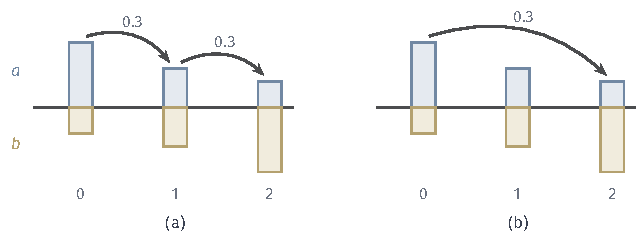
\includegraphics[width=108mm]{figures/07-probability/07-distribution-optimization/tikz/ot-supply-arrows/figure.pdf}
 \caption{全章例子：蓝柱向上是源质量$\bm{a}=(0.5,0.3,0.2)$，黄柱向下是目标质量$\bm{b}=(0.2,0.3,0.5)$，位置为$0,1,2$；箭头上的数是搬运的质量，未画箭头的质量留在原地。(a)逐格搬运，平方成本$0.6$。(b)跳格搬运，平方成本$1.2$。}
 \label{fig:ot-supply-arrows}
\end{BookInlineFigure}

还有许多别的搬法。最“不动脑筋”的是独立搬运：从$x_i$出发的质量按$\bm{b}$的比例分给各个目标，$\pi_{i,j}=a_ib_j$。图~\ref{fig:ot-plan-tables}把三个方案写成表，它们的行和、列和完全相同，平方成本却分别是$1.58$、$1.2$和$0.6$。同一对边缘分布，因质量配对方式不同而产生不同成本；本章的问题就是在全部配对方式中找成本最低的那一个。

\begin{BookInlineFigure}
 \centering
 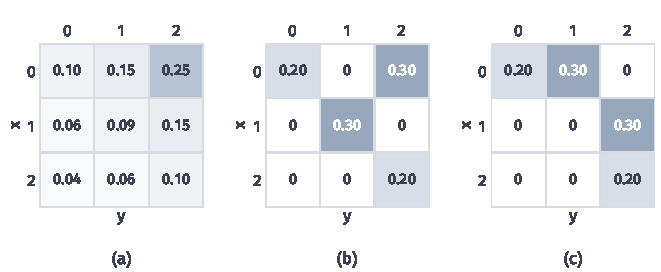
\includegraphics[width=112mm]{figures/07-probability/07-distribution-optimization/matplotlib/ot-plan-tables/figure.pdf}
 \caption{全章例子的三个运输方案，行是源位置$x$，列是目标位置$y$，颜色越深质量越大。三张表的行和都是$\bm{a}$，列和都是$\bm{b}$。(a)独立方案$\pi_{i,j}=a_ib_j$，平方成本$1.58$。(b)跳格搬运，平方成本$1.2$。(c)逐格搬运，平方成本$0.6$。}
 \label{fig:ot-plan-tables}
\end{BookInlineFigure}

这里有三个不同的问题。其一，在全部满足行列约束的方案中优化，允许把一个位置的质量拆开送往几处，这是耦合上的优化。其二，要求每个源位置的质量整体送到一个目标位置，这是运输映射上的优化，可行的方案少得多，甚至可能没有。其三，确认最低成本确实被某个方案取到，而不只是一个无法达到的下确界。下面三小节依次处理。把最低成本当作分布之间的距离时，它的对称性、三角不等式以及与弱收敛的关系已在第~\ref{chap:distribution-comparison}章讨论，本章不再重复。

\subsection{固定边缘的耦合}
\label{sec:ot-couplings}

有限情形的方案是一张非负表。设源有$m$个位置，质量向量$\bm{a}\in\mathbb{R}^{m}$；目标有$n$个位置，质量向量$\bm{b}\in\mathbb{R}^{n}$；两者都非负且总和为$1$。可行方案的全体是
\begin{equation}
 U(\bm{a},\bm{b})=\bigl\{\bm{\pi}\in\mathbb{R}^{m\times n}:\ \bm{\pi}\geq0,\ \bm{\pi}\bm{1}=\bm{a},\ \bm{\pi}^{\top}\bm{1}=\bm{b}\bigr\},
 \label{eq:ot-transport-polytope}
\end{equation}
其中$\bm{\pi}\geq0$指每个元素非负，$\bm{1}$是全一向量。它由有限个线性等式和不等式刻画，是一个有界的凸多面体，称为\term{运输多面体}（transport polytope）。总成本是线性函数
\[
 \langle\bm{C},\bm{\pi}\rangle=\sum_{i,j}c_{i,j}\pi_{i,j} .
\]

把$\bm{\pi}$看成取值于$\{x_i\}\times\{y_j\}$的随机向量$(X,Y)$的联合概率表，行和、列和约束就是“$X$的边缘为$\bm{a}$，$Y$的边缘为$\bm{b}$”，总成本就是$\mathbb{E}[c(X,Y)]$。这正是第~\ref{chap:distribution-comparison}章的耦合：$\mathcal{X}$上的分布$\mu$与$\mathcal{Y}$上的分布$\nu$的耦合是$\mathcal{X}\times\mathcal{Y}$上边缘分别为$\mu,\nu$的分布，全体记作$\Pi(\mu,\nu)$。有限情形$\Pi(\mu,\nu)$与$U(\bm{a},\bm{b})$一一对应。一般情形不再有表，但问题的写法不变。

\begin{definition}[最优运输问题]
\label{def:ot-problem}
设$\mu,\nu$分别是$\mathcal{X},\mathcal{Y}$上的概率分布，$c:\mathcal{X}\times\mathcal{Y}\to[0,\infty]$可测。对耦合$\pi\in\Pi(\mu,\nu)$，称$\int c\,\mathrm{d}\pi$为它的运输成本。称
\begin{equation}
 \operatorname{OT}_c(\mu,\nu)=\inf_{\pi\in\Pi(\mu,\nu)}\int_{\mathcal{X}\times\mathcal{Y}}c(x,y)\,\pi(\mathrm{d}x,\mathrm{d}y)
 \label{eq:ot-kantorovich}
\end{equation}
为\term{最优运输问题}（optimal transport problem）的最优值。耦合也称为\term{运输方案}（transport plan）；达到下确界的耦合称为\term{最优耦合}（optimal coupling）。
\end{definition}

定义要求成本非负，是为了让每个耦合的成本都有意义：非负可测函数的积分总有定义，取值在$[0,\infty]$中，不会出现$\infty-\infty$。若成本有界或下方被可积函数控制，也可以同样处理，但本章只用非负成本。取$\mathcal{X}=\mathcal{Y}$为度量空间、$c=d^{p}$时，$\operatorname{OT}_c^{1/p}$就是第~\ref{chap:distribution-comparison}章的$W_p$。

可行集合从不为空：乘积分布$\mu\otimes\nu$总是一个耦合，它对应“让$X$与$Y$独立”，在有限情形就是图~\ref{fig:ot-plan-tables}(a)的独立方案。但可行不等于有有限成本的方案。取$\mu=\delta_0$，$\nu$为标准Cauchy分布，$c(x,y)=(x-y)^{2}$。$\mu$只有一个点，任何耦合的第一个分量都恒为$0$，所以$\Pi(\mu,\nu)$只有$\delta_0\otimes\nu$一个元素。Cauchy密度与$1/(1+y^{2})$成正比，乘以$y^{2}$后在远处趋于正常数，所以这个唯一耦合的成本是
\[
 \int y^{2}\,\nu(\mathrm{d}y)=\infty .
\]
最优值是$\infty$，问题虽然可行，却给不出任何有用的比较。对$c=\lvert x-y\rvert^{p}$，只要两个分布都有有限$p$阶矩，第~\ref{chap:distribution-comparison}章的估计就说明独立耦合的成本有限；本章讨论的具体问题都满足这类条件。

\subsection{运输映射}
\label{sec:ot-maps}

耦合允许把一个点的质量拆开。如果规定每个源点的质量必须整体送到同一个目标点，方案就由一个函数$T:\mathcal{X}\to\mathcal{Y}$描述：$x$处的质量全部送到$T(x)$。目标处收到的质量分布是$\mu$在$T$下的推前$T_\#\mu$，即$T_\#\mu(B)=\mu(T^{-1}(B))$，推前测度的一般性质可参考\BookChapterRef{chap:pushforward-measures}{卷四第9章“推前测度”}。满足
\begin{equation}
 T_\#\mu=\nu
 \label{eq:ot-transport-map}
\end{equation}
的可测映射称为从$\mu$到$\nu$的\term{运输映射}（transport map）。在映射中优化成本$\int c(x,T(x))\,\mu(\mathrm{d}x)$称为\term{Monge问题}（Monge problem）。

映射是耦合的特例。设$X\sim\mu$，令$Y=T(X)$，则$(X,Y)$的联合分布是
\[
 \pi_T=(\mathrm{id},T)_\#\mu ,
\]
它把全部质量放在$T$的图像$\{(x,T(x))\}$上。它的第一个边缘是$\mu$，第二个边缘是$T_\#\mu=\nu$，所以$\pi_T\in\Pi(\mu,\nu)$，并且$\int c\,\mathrm{d}\pi_T=\mathbb{E}[c(X,T(X))]$。于是Monge问题的下确界不小于$\operatorname{OT}_c(\mu,\nu)$：映射能做的，耦合都能做。

反过来不成立，而且差别可能是根本性的。取$\mu=\delta_0$，$\nu=\tfrac12\delta_{-1}+\tfrac12\delta_1$。任何映射都把$\delta_0$推成单点分布$\delta_{T(0)}$，不可能等于有两个原子的$\nu$，所以映射问题连可行解都没有。耦合问题却有唯一的可行解$\delta_0\otimes\nu$：$0$处的单位质量一分为二，各送一半到$\pm1$，见图~\ref{fig:ot-split-map}(a)。

\begin{BookInlineFigure}
 \centering
 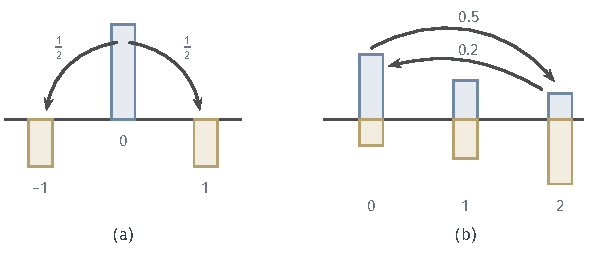
\includegraphics[width=100mm]{figures/07-probability/07-distribution-optimization/tikz/ot-split-map/figure.pdf}
 \caption{映射与耦合。(a)$\delta_0$到$\tfrac12\delta_{-1}+\tfrac12\delta_1$：唯一的耦合把单位质量拆成两半，没有映射能做到。(b)全章例子中唯一的运输映射$T(0)=2$，$T(1)=1$，$T(2)=0$，平方成本$2.8$。}
 \label{fig:ot-split-map}
\end{BookInlineFigure}

全章例子中映射是存在的，但选择极少。$T$把每个源位置的整份质量送到一个目标位置，所以每个$b_j$必须等于若干个$a_i$之和。$b_0=0.2$只能由$a_2=0.2$凑成，$b_1=0.3$只能由$a_1$凑成，剩下$a_0=0.5$正好是$b_2$，于是唯一的映射是$T(0)=2$，$T(1)=1$，$T(2)=0$，平方成本$0.5\cdot4+0.2\cdot4=2.8$，见图~\ref{fig:ot-split-map}(b)。它比逐格搬运的$0.6$贵得多，因为逐格搬运必须把$0$处的$0.5$拆成$0.2$与$0.3$。有限分布之间的映射问题受制于质量能否恰好凑整，耦合问题则没有这个障碍。

\subsection{最优耦合的存在}
\label{sec:ot-existence}

下确界$\operatorname{OT}_c(\mu,\nu)$是否被某个耦合取到？先看有限情形。

\paragraph{有限支持}
运输多面体$U(\bm{a},\bm{b})$非空（含$\bm{a}\bm{b}^{\top}$），是闭集（由等式和非负性定义），并且有界（每个元素在$[0,1]$中），所以是$\mathbb{R}^{m\times n}$中的紧集。成本矩阵各元素有限时，$\langle\bm{C},\bm{\pi}\rangle$是$\bm{\pi}$的连续函数，紧集上的连续函数取到最小值，所以最优方案存在。

图~\ref{fig:ot-polytope}用一个能画出来的例子说明这一点。取$\bm{a}=(0.4,0.6)$位于$x=0,2$，$\bm{b}=(0.2,0.3,0.5)$位于$y=0,1,2$，成本$(x-y)^{2}$。$2\times3$的方案由左上两个元素$s=\pi_{1,1}$、$t=\pi_{1,2}$确定（这里行列下标从$1$起），其余元素是
\[
 \pi_{1,3}=0.4-s-t,\qquad \pi_{2,1}=0.2-s,\qquad \pi_{2,2}=0.3-t,\qquad \pi_{2,3}=0.1+s+t .
\]
非负性给出$0\leq s\leq0.2$，$0\leq t\leq0.3$，$s+t\leq0.4$，这是一个五边形。成本化成
\[
 \langle\bm{C},\bm{\pi}\rangle=t+4(0.4-s-t)+4(0.2-s)+(0.3-t)=2.7-8s-4t ,
\]
等值线是一族平行直线，最小值$0.3$在顶点$(s,t)=(0.2,0.2)$处取得。线性目标在多面体上的最小值总能在顶点处取到，这是线性规划的基本事实，第~\ref{sec:ot-discrete}节还会用到。

\begin{BookInlineFigure}
 \centering
 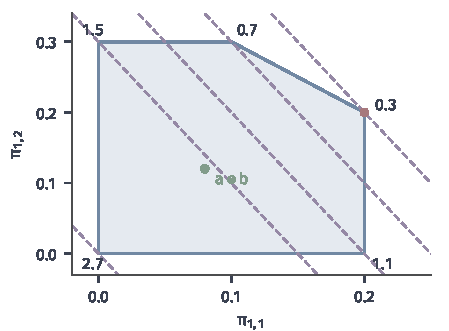
\includegraphics[width=76mm]{figures/07-probability/07-distribution-optimization/matplotlib/ot-polytope/figure.pdf}
 \caption{$\bm{a}=(0.4,0.6)$、$\bm{b}=(0.2,0.3,0.5)$的运输多面体，坐标是$\pi_{1,1}$与$\pi_{1,2}$。浅蓝五边形是可行集，顶点旁的数是该顶点的平方成本；紫色虚线是成本$2.7-8s-4t$的等值线；绿点是独立方案（成本$1.58$），红点是最优顶点（成本$0.3$）。}
 \label{fig:ot-polytope}
\end{BookInlineFigure}

\paragraph{欧氏空间上的分布}
一般分布的耦合集合是无穷维的，需要换一种紧性。第~\ref{chap:weak-convergence-of-distributions}章证明了：$\mathbb{R}^{d}$上一族分布胎紧，则其中任一序列都有弱收敛子列。我们要说明耦合集合正好胎紧，而且弱极限仍是耦合；再说明成本随耦合的变化是下半连续的，即极限处的成本不会突然变大。

\begin{lemma}[耦合集合的紧性]
\label{lem:ot-coupling-compact}
设$\mu,\nu$分别是$\mathbb{R}^{m},\mathbb{R}^{n}$上的概率分布。则$\Pi(\mu,\nu)$胎紧；若$\pi_k\in\Pi(\mu,\nu)$且$\pi_k\xrightarrow{\mathrm{w}}\pi$，则$\pi\in\Pi(\mu,\nu)$。
\end{lemma}

\begin{proof}
任给$\varepsilon>0$。单个分布是胎紧的，取紧集$K_1\subset\mathbb{R}^{m}$与$K_2\subset\mathbb{R}^{n}$，使$\mu(K_1^{\mathrm{c}})<\varepsilon/2$，$\nu(K_2^{\mathrm{c}})<\varepsilon/2$。$K_1\times K_2$是紧集，并且它的补集含于$(K_1^{\mathrm{c}}\times\mathbb{R}^{n})\cup(\mathbb{R}^{m}\times K_2^{\mathrm{c}})$。于是对每个耦合$\pi$，
\[
 \pi\bigl((K_1\times K_2)^{\mathrm{c}}\bigr)\leq\mu(K_1^{\mathrm{c}})+\nu(K_2^{\mathrm{c}})<\varepsilon .
\]
同一个紧集对全部耦合都适用，所以$\Pi(\mu,\nu)$胎紧。

再看弱极限。任取$\mathbb{R}^{m}$上的有界连续函数$h$，函数$(x,y)\mapsto h(x)$在$\mathbb{R}^{m+n}$上有界连续。由弱收敛与第一边缘为$\mu$，
\[
 \int h(x)\,\pi(\mathrm{d}x,\mathrm{d}y)=\lim_{k\to\infty}\int h(x)\,\pi_k(\mathrm{d}x,\mathrm{d}y)=\int h\,\mathrm{d}\mu .
\]
所以$\pi$的第一边缘与$\mu$对一切有界连续函数的积分相同，两者相等。第二边缘同理。
\end{proof}

\begin{lemma}[成本的下半连续性]
\label{lem:ot-cost-lsc}
设$c:\mathbb{R}^{m}\times\mathbb{R}^{n}\to[0,\infty]$是下半连续函数，即对每个点$z$与每个$z_k\to z$有$c(z)\leq\liminf_kc(z_k)$。若概率分布$\pi_k\xrightarrow{\mathrm{w}}\pi$，则
\begin{equation}
 \int c\,\mathrm{d}\pi\leq\liminf_{k\to\infty}\int c\,\mathrm{d}\pi_k .
 \label{eq:ot-cost-lsc}
\end{equation}
\end{lemma}

\begin{proof}
弱收敛只对有界连续函数给出积分的收敛，所以先用有界连续函数从下方逼近$c$。对正整数$j$，令
\[
 c_j(z)=\min\Bigl\{j,\ \inf_{w}\bigl(c(w)+j\lVert z-w\rVert_2\bigr)\Bigr\}.
\]
取$w=z$知$c_j\leq c$；$c_j$关于$j$单调不减，取值在$[0,j]$中。每个$z\mapsto c(w)+j\lVert z-w\rVert_2$都满足$j$-Lipschitz条件，它们的下确界以及与常数$j$的较小者也满足，所以$c_j$连续。

再证$c_j(z)\to c(z)$。任取实数$s<c(z)$。由下半连续，存在$r>0$，使$\lVert w-z\rVert_2<r$时$c(w)>s$。于是对一切$w$，或者$c(w)>s$，或者$j\lVert z-w\rVert_2\geq jr$。当$j\geq\max(s/r,\,s)$时，两种情形下都有
\[
 c(w)+j\lVert z-w\rVert_2\geq s ,
\]
从而$c_j(z)\geq s$。$s$可以任意接近$c(z)$（$c(z)=\infty$时可以任意大），所以$c_j(z)\uparrow c(z)$。

对固定的$j$，$c_j$有界连续，由弱收敛与$c_j\leq c$，
\[
 \int c_j\,\mathrm{d}\pi=\lim_{k\to\infty}\int c_j\,\mathrm{d}\pi_k\leq\liminf_{k\to\infty}\int c\,\mathrm{d}\pi_k .
\]
令$j\to\infty$，由单调收敛定理，左边趋于$\int c\,\mathrm{d}\pi$，得到式~\eqref{eq:ot-cost-lsc}。
\end{proof}

\begin{theorem}[最优耦合的存在]
\label{thm:ot-existence}
设$\mu,\nu$分别是$\mathbb{R}^{m},\mathbb{R}^{n}$上的概率分布，$c:\mathbb{R}^{m}\times\mathbb{R}^{n}\to[0,\infty]$下半连续。则存在$\pi^{*}\in\Pi(\mu,\nu)$，使
\begin{equation}
 \int c\,\mathrm{d}\pi^{*}=\operatorname{OT}_c(\mu,\nu).
 \label{eq:ot-existence}
\end{equation}
\end{theorem}

\begin{proof}
若$\operatorname{OT}_c(\mu,\nu)=\infty$，每个耦合都达到它。下设它有限，取耦合列$\pi_k$，使其成本递减地趋于$\operatorname{OT}_c(\mu,\nu)$。由引理~\ref{lem:ot-coupling-compact}，这列耦合胎紧，由第~\ref{chap:weak-convergence-of-distributions}章的弱收敛子列定理，存在子列$\pi_{k_l}\xrightarrow{\mathrm{w}}\pi^{*}$，并且$\pi^{*}\in\Pi(\mu,\nu)$。由引理~\ref{lem:ot-cost-lsc}，
\[
 \int c\,\mathrm{d}\pi^{*}\leq\liminf_{l\to\infty}\int c\,\mathrm{d}\pi_{k_l}=\operatorname{OT}_c(\mu,\nu).
\]
反向不等式由下确界的定义成立。
\end{proof}

定理的两个条件各有分工。固定边缘使耦合集合胎紧，这是“极小化序列有收敛子列”的来源；下半连续使成本在极限处不会跳高，这是“极限仍是最小者”的来源。$\mathbb{R}^{d}$可以换成一般的完备可分度量空间，证明相同，只是要用一般形式的Prokhorov定理，可查阅~\scite{math-villani2009transport}。

\paragraph{去掉下半连续性}
下面的例子说明下半连续不能省。取$\mu=\nu=\operatorname{Unif}(0,1)$，成本在对角线上取$1$，在对角线外取距离：
\[
 c(x,y)=\begin{cases}1, & x=y,\\ \lvert x-y\rvert, & x\neq y .\end{cases}
\]
它在对角线上不是下半连续的：$c(x,x)=1$，而附近的$c(x,x+h)=\lvert h\rvert\to0$。对$0<h<1$，令$X\sim\operatorname{Unif}(0,1)$，$Y=X+h$（若超过$1$则减去$1$）。$Y$仍服从$\operatorname{Unif}(0,1)$，$X\neq Y$，并且$\lvert X-Y\rvert$以概率$1-h$等于$h$、以概率$h$等于$1-h$，所以成本是
\[
 (1-h)h+h(1-h)=2h(1-h)\to0\qquad(h\to0).
\]
于是$\operatorname{OT}_c(\mu,\nu)=0$。但没有耦合的成本为$0$：若$\pi$在对角线上有正质量，成本至少是这部分质量；若没有，$\pi$的质量全在$\{x\neq y\}$上，$\lvert x-y\rvert>0$处处成立，积分为正。极小化序列弱收敛到对角线上的耦合，成本却在极限处跳到$1$。

\paragraph{耦合存在而映射不达到}
定理只保证最优耦合存在。即使最优耦合存在，Monge问题的下确界也可能取不到。在$\mathbb{R}^{2}$中取$\mu$为线段$\{0\}\times[0,1]$上的均匀分布，$\nu$把一半质量均匀放在$\{-1\}\times[0,1]$上，另一半均匀放在$\{1\}\times[0,1]$上，成本为平方欧氏距离。任何耦合都要把每份质量横向移动距离$1$，所以成本至少为$1$；把每个点的质量平分到左右两侧同一高度，成本恰为$1$，是最优耦合。

映射却做不到$1$。把$[0,1]$等分成$n$段，每段的下半段水平送到左侧、上半段送到右侧，并在竖直方向拉伸两倍铺满该段，得到映射$T_n$。竖直位移在每半段上均匀分布在长为$1/(2n)$的区间里，平均平方为$1/(12n^{2})$，所以$T_n$的成本是
\[
 1+\frac{1}{12n^{2}}\to1 ,
\]
见图~\ref{fig:ot-monge-stripes}。若某个映射$T$的成本恰为$1$，竖直位移必须几乎处处为零，即$T(0,s)=(\pm1,s)$。记$L$为送往左侧的高度集合，左侧收到的质量中高度落在$L$里的部分是$\lvert L\rvert$，而$\nu$要求它是$\lvert L\rvert/2$，所以$\lvert L\rvert=0$；左侧总共却必须收到$1/2$，矛盾。

\begin{BookInlineFigure}
 \centering
 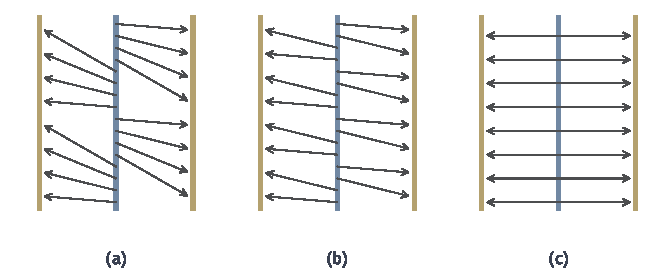
\includegraphics[width=112mm]{figures/07-probability/07-distribution-optimization/matplotlib/ot-monge-stripes/figure.pdf}
 \caption{蓝色竖线是$\mu$（$\{0\}\times[0,1]$上均匀），两条黄色竖线各带$\nu$的一半质量。(a)$n=2$的条带映射$T_2$，成本$1+1/48$。(b)$n=4$的条带映射，成本$1+1/192$。(c)最优耦合把每个点的质量平分到两侧，成本$1$，任何映射都达不到。}
 \label{fig:ot-monge-stripes}
\end{BookInlineFigure}

所以“最优方案存在”只针对耦合。最优耦合能否由映射实现，以及是否唯一，都要另加条件，第~\ref{sec:ot-concrete}节会在具体问题中看到这些条件。

\section{最优性的判别}
\label{sec:ot-optimality}

图~\ref{fig:ot-plan-tables}(c)的逐格搬运成本是$0.6$。怎样确信没有更便宜的方案？逐个比较做不到，可行方案有无穷多个。每个可行方案只给出最优值的一个上界；要证实某个方案最优，还需要一个对一切可行方案都成立的下界，并且它恰好等于这个方案的成本。本节先构造这样的下界，再说明它在什么条件下能与原问题的最优值相等。

\subsection{对偶势}
\label{sec:ot-potentials}

先在有限情形找下界。设想有人提出一组价格：在源位置$x_i$交出一份质量可得收入$f_i$，在目标位置$y_j$收下一份质量可得收入$g_j$。若价格满足
\[
 f_i+g_j\leq c_{i,j}\qquad\text{对一切}\ i,j ,
\]
则无论按什么方案搬运，每份质量带来的收入都不超过它的运费。把行和约束乘以$f_i$、列和约束乘以$g_j$再相加，对任意$\bm{\pi}\in U(\bm{a},\bm{b})$，
\[
 \sum_ia_if_i+\sum_jb_jg_j=\sum_{i,j}\pi_{i,j}(f_i+g_j)\leq\sum_{i,j}\pi_{i,j}c_{i,j} .
\]
左边不依赖方案，所以它是所有可行方案成本的一个公共下界。一般分布的写法相同，只是把向量换成函数。

\begin{definition}[对偶势]
\label{def:ot-potentials}
设$\mu,\nu$与成本$c\geq0$如定义~\ref{def:ot-problem}。若$\varphi\in L^{1}(\mu)$，$\psi\in L^{1}(\nu)$，并且
\begin{equation}
 \varphi(x)+\psi(y)\leq c(x,y)\qquad\text{对一切}\ x\in\mathcal{X},\ y\in\mathcal{Y},
 \label{eq:ot-dual-constraint}
\end{equation}
则称$(\varphi,\psi)$为一对可行的\term{对偶势}（dual potentials），称
\begin{equation}
 J(\varphi,\psi)=\int\varphi\,\mathrm{d}\mu+\int\psi\,\mathrm{d}\nu
 \label{eq:ot-dual-value}
\end{equation}
为它的对偶值。
\end{definition}

对偶势里的$\varphi,\psi$可以取负值，只要求可积；这样它们的积分有限，后面的相减才有意义。下面的定理把“价格”论证写成一般形式，并且给出原对偶值之差的精确表达式。

\begin{theorem}[弱对偶与原对偶差]
\label{thm:ot-weak-duality}
设$(\varphi,\psi)$是可行的对偶势，$\pi\in\Pi(\mu,\nu)$。则
\begin{equation}
 \int c\,\mathrm{d}\pi-J(\varphi,\psi)=\int\bigl(c(x,y)-\varphi(x)-\psi(y)\bigr)\,\pi(\mathrm{d}x,\mathrm{d}y)\geq0 ,
 \label{eq:ot-gap}
\end{equation}
两边可以同时为$+\infty$。于是$J(\varphi,\psi)\leq\operatorname{OT}_c(\mu,\nu)$。若某个$\pi$与$(\varphi,\psi)$使式~\eqref{eq:ot-gap}为零，则$\pi$是最优耦合，$(\varphi,\psi)$使对偶值最大。
\end{theorem}

\begin{proof}
由于$\pi$的第一边缘是$\mu$，对可积的$\varphi$有
\[
 \int\varphi(x)\,\pi(\mathrm{d}x,\mathrm{d}y)=\int\varphi\,\mathrm{d}\mu .
\]
这对示性函数是边缘的定义，对简单函数由线性性成立，对非负函数由单调收敛定理成立，再对正负部分分别使用即得可积情形。$\psi$同理。

记松弛量$s(x,y)=c(x,y)-\varphi(x)-\psi(y)$，由式~\eqref{eq:ot-dual-constraint}它非负，积分有定义。$c=s+\varphi+\psi$中后两项关于$\pi$可积，所以
\[
 \int c\,\mathrm{d}\pi=\int s\,\mathrm{d}\pi+\int\varphi\,\mathrm{d}\mu+\int\psi\,\mathrm{d}\nu ,
\]
这就是式~\eqref{eq:ot-gap}。对$\pi$取下确界得$J(\varphi,\psi)\leq\operatorname{OT}_c(\mu,\nu)$。若差为零，$\pi$的成本等于一个下界，不可能有成本更低的耦合；对任何别的可行对偶势$(\varphi',\psi')$，由刚证明的不等式，$J(\varphi',\psi')$不超过$\int c\,\mathrm{d}\pi$，而后者等于$J(\varphi,\psi)$。
\end{proof}

式~\eqref{eq:ot-gap}的右边只看$\pi$把质量放在哪里：放在松弛量为零的地方不贡献差，放在松弛量为正的地方按松弛量计差。所以候选方案$\pi$的最优性可以这样核验：找一对可行的对偶势，检查$\pi$的质量是否几乎全部落在等号集合$\{c=\varphi+\psi\}$上。这一条件称为互补松弛。

\paragraph{例子的证据}
回到全章例子。取
\[
 \bm{f}=(0,\ -1,\ -2),\qquad \bm{g}=(0,\ 1,\ 2),
\]
则$f_i+g_j=j-i$。成本$(i-j)^{2}$与它的差就是松弛矩阵
\[
 \bm{S}=\bm{C}-\bigl(f_i+g_j\bigr)_{i,j}=\begin{bmatrix}0&0&2\\2&0&0\\6&2&0\end{bmatrix}.
\]
各元素非负，所以$(\bm{f},\bm{g})$可行；对偶值为
\[
 \langle\bm{a},\bm{f}\rangle+\langle\bm{b},\bm{g}\rangle=(-0.3-0.4)+(0.3+1.0)=0.6 .
\]
逐格搬运的质量放在$(0,0),(0,1),(1,2),(2,2)$上，这四处的松弛量都是$0$，于是它的成本$0.6$等于这个下界，它是最优方案。

同一对势也给出其他方案离最优有多远。由式~\eqref{eq:ot-gap}，跳格搬运把$0.3$放在松弛量为$2$的$(0,2)$处，所以
\[
 1.2-0.6=0.3\times2 .
\]
独立方案在每个格子上都有质量，它与最优值之差是$\sum_{i,j}a_ib_js_{i,j}$，逐项相加得
\[
 0.25\times2+0.06\times2+0.04\times6+0.06\times2=0.98=1.58-0.6 .
\]
图~\ref{fig:ot-dual-envelope}(b)画出松弛矩阵，红圈标出最优方案的质量所在。

\paragraph{由一个势求另一个势}
给定$\bm{g}$，满足约束的$f_i$最大能取多少？约束$f_i\leq c_{i,j}-g_j$对每个$j$成立，所以最大可取
\begin{equation}
 f_i=\min_{j}\bigl(c_{i,j}-g_j\bigr).
 \label{eq:ot-c-transform}
\end{equation}
这称为$\bm{g}$的\term{$c$变换}（$c$-transform）；一般情形写成$\psi^{c}(x)=\inf_y\bigl(c(x,y)-\psi(y)\bigr)$。对偶值关于$\bm{f}$单调增加，所以最优的$\bm{f}$总可以取成$\bm{g}$的$c$变换。几何上，它是一族曲线$x\mapsto c(x,y_j)-g_j$的下包络。图~\ref{fig:ot-dual-envelope}(a)对例子中的$\bm{g}=(0,1,2)$画出三条抛物线$(x-j)^{2}-j$与它们的下包络，在$x=0,1,2$处恰好取到$\bm{f}=(0,-1,-2)$。

\begin{BookInlineFigure}
 \centering
 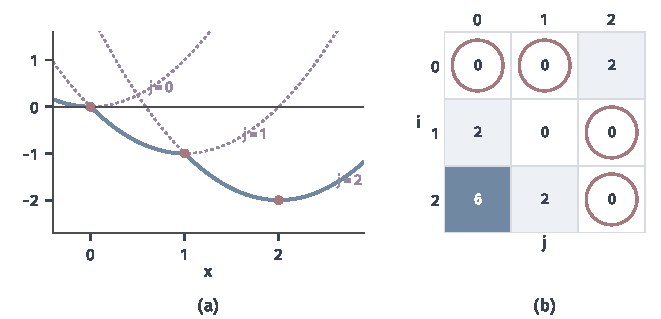
\includegraphics[width=112mm]{figures/07-probability/07-distribution-optimization/matplotlib/ot-dual-envelope/figure.pdf}
 \caption{全章例子的对偶势。(a)紫色点线是$(x-j)^{2}-g_j$，$\bm{g}=(0,1,2)$；蓝线是它们的下包络，即$\bm{g}$的$c$变换；红点是$f_i$。(b)松弛量$c_{i,j}-f_i-g_j$，红圈是逐格搬运方案的非零位置，全部落在零松弛处。}
 \label{fig:ot-dual-envelope}
\end{BookInlineFigure}

成本取度量$d$时，$c$变换产生第~\ref{chap:distribution-comparison}章的Lipschitz函数：$\psi^{c}(x)=\inf_y(d(x,y)-\psi(y))$是一族$1$-Lipschitz函数的下确界，本身也是$1$-Lipschitz函数。再对一个$1$-Lipschitz函数$h$求$c$变换，由$h(y)-h(x)\leq d(x,y)$得$\inf_y(d(x,y)-h(y))\geq-h(x)$，取$y=x$取等，结果恰为$-h$。所以对偶势可以取成$(-h,h)$的形式，对偶值是$\mathbb{E}_{\nu}[h]-\mathbb{E}_{\mu}[h]$；Kantorovich--Rubinstein对偶正是一般对偶在$c=d$时的这一特殊形式。

最优势一般不唯一。例子中把$\bm{f}$加上常数$t$、$\bm{g}$减去$t$，对偶值不变；即使固定$f_0=0$，可行最优势也不止一组。由零松弛的四个位置得$g_0=0$，$g_1=1$，$g_2=1-f_1$，$f_2=f_1-1$，再检查其余五个约束，得到$-3\leq f_1\leq-1$，其中每个$f_1$都给出对偶值$0.6$。最优方案唯一（第~\ref{sec:ot-one-dimensional}节将证明），证明它最优的价格却有许多组。

\subsection{强对偶的条件}
\label{sec:ot-strong-duality}

弱对偶只给出不等式。要用对偶势证实最优性，还需要知道下界能够逼近甚至等于最优值，即两个问题之间没有\term{对偶间隙}（duality gap）。先证明有限情形。

\begin{theorem}[有限运输问题的强对偶]
\label{thm:ot-finite-duality}
设$\bm{a}\in\mathbb{R}^{m}$，$\bm{b}\in\mathbb{R}^{n}$是概率向量，$\bm{C}\in\mathbb{R}^{m\times n}$。则
\begin{equation}
 \min_{\bm{\pi}\in U(\bm{a},\bm{b})}\langle\bm{C},\bm{\pi}\rangle=\max\Bigl\{\langle\bm{a},\bm{f}\rangle+\langle\bm{b},\bm{g}\rangle:\ f_i+g_j\leq c_{i,j}\ \text{对一切}\ i,j\Bigr\},
 \label{eq:ot-finite-duality}
\end{equation}
两边的最小值与最大值都能取到。
\end{theorem}

\begin{proof}
把$\bm{\pi}$的$mn$个元素看成变量。原问题是线性规划：在等式约束$\sum_j\pi_{i,j}=a_i$（$m$个）、$\sum_i\pi_{i,j}=b_j$（$n$个）和$\pi_{i,j}\geq0$下最小化$\sum_{i,j}c_{i,j}\pi_{i,j}$。给前$m$个等式配乘子$f_i$，后$n$个配乘子$g_j$，Lagrange函数是
\[
 \sum_{i,j}c_{i,j}\pi_{i,j}+\sum_if_i\Bigl(a_i-\sum_j\pi_{i,j}\Bigr)+\sum_jg_j\Bigl(b_j-\sum_i\pi_{i,j}\Bigr).
\]
整理成
\[
 \langle\bm{a},\bm{f}\rangle+\langle\bm{b},\bm{g}\rangle+\sum_{i,j}\bigl(c_{i,j}-f_i-g_j\bigr)\pi_{i,j} .
\]
对$\pi_{i,j}\geq0$取下确界，只有当每个系数$c_{i,j}-f_i-g_j$都非负时下确界才有限，等于$\langle\bm{a},\bm{f}\rangle+\langle\bm{b},\bm{g}\rangle$。所以对偶线性规划正是式~\eqref{eq:ot-finite-duality}右边。

原问题可行（含$\bm{a}\bm{b}^{\top}$），目标值不小于$\min_{i,j}c_{i,j}$，有下界。由线性规划的强对偶定理，原问题与对偶问题都有最优解，并且最优值相等，可参考\BookChapterRef{chap:linear-programming}{卷五第2章“线性规划”}。
\end{proof}

第~\ref{chap:distribution-comparison}章证明有限支撑的Kantorovich--Rubinstein对偶，用的正是这个定理。一般分布不能直接套用线性规划，但在紧致空间上可以用有限问题去逼近。

\begin{theorem}[紧致空间上的强对偶]
\label{thm:ot-compact-duality}
设$(\mathcal{X},d_{\mathcal{X}})$，$(\mathcal{Y},d_{\mathcal{Y}})$是紧致度量空间，$c:\mathcal{X}\times\mathcal{Y}\to[0,\infty)$连续，$\mu,\nu$分别是其上的Borel概率分布。则
\begin{equation}
 \operatorname{OT}_c(\mu,\nu)=\sup\bigl\{J(\varphi,\psi):\ (\varphi,\psi)\ \text{是有界可测的可行对偶势}\bigr\}.
 \label{eq:ot-compact-duality}
\end{equation}
\end{theorem}

\begin{proof}
由定理~\ref{thm:ot-weak-duality}，右边不超过左边，只需对每个$\eta>0$构造对偶值不小于$\operatorname{OT}_c(\mu,\nu)-3\eta$的可行势。

\emph{第一步：选尺度。}$\mathcal{X}\times\mathcal{Y}$紧致，$c$在其上一致连续：存在$\delta>0$，使$d_{\mathcal{X}}(x,x')<\delta$且$d_{\mathcal{Y}}(y,y')<\delta$时$\lvert c(x,y)-c(x',y')\rvert\leq\eta$。

\emph{第二步：离散化。}紧致空间可被有限个半径$\delta/2$的球覆盖，依次去掉与前面重叠的部分并丢弃空集，得到$\mathcal{X}$的有限Borel划分$A_1,\dots,A_m$，每块直径小于$\delta$；同样得到$\mathcal{Y}$的划分$B_1,\dots,B_n$。在每块中取一个代表点$x_i\in A_i$，$y_j\in B_j$，令
\[
 a_i=\mu(A_i),\qquad b_j=\nu(B_j),\qquad c_{i,j}=c(x_i,y_j).
\]
由定理~\ref{thm:ot-finite-duality}，离散问题有最优方案$\bm{\pi}^{\delta}$与最优对偶解$(\bm{f},\bm{g})$，两者的值相等，记为$V_\delta$。

\emph{第三步：离散问题不比原问题贵太多。}把离散方案铺回原空间：在$A_i\times B_j$上放入质量$\pi^{\delta}_{i,j}$，并按$\mu$与$\nu$在这两块上的形状分布，即
\[
 \pi=\sum_{i,j:\ a_i>0,\ b_j>0}\pi^{\delta}_{i,j}\,\frac{\mu|_{A_i}}{a_i}\otimes\frac{\nu|_{B_j}}{b_j} .
\]
（$a_i=0$时第$i$行全为零，可以略去。）由行和$\sum_j\pi^{\delta}_{i,j}=a_i$，它的第一边缘是
\[
 \sum_i\Bigl(\sum_j\pi^{\delta}_{i,j}\Bigr)\frac{\mu|_{A_i}}{a_i}=\sum_i\mu|_{A_i}=\mu ,
\]
第二边缘同理是$\nu$，所以$\pi\in\Pi(\mu,\nu)$。在$A_i\times B_j$上$c\leq c_{i,j}+\eta$，于是
\[
 \operatorname{OT}_c(\mu,\nu)\leq\int c\,\mathrm{d}\pi\leq V_\delta+\eta .
\]

\emph{第四步：把离散势扩展成函数。}令
\[
 \varphi(x)=\min_{j}\bigl(c(x,y_j)-g_j\bigr),\qquad \psi(y)=g_j-\eta\quad(y\in B_j).
\]
$\varphi$是有限个连续函数的最小值，$\psi$是简单函数，都有界可测。可行性：对$y\in B_j$，$\lvert c(x,y_j)-c(x,y)\rvert\leq\eta$，所以
\[
 \varphi(x)+\psi(y)\leq c(x,y_j)-g_j+g_j-\eta\leq c(x,y).
\]
对偶值：对$x\in A_i$，$c(x,y_j)\geq c_{i,j}-\eta$，又由离散对偶可行性$c_{i,j}-g_j\geq f_i$，所以$\varphi(x)\geq f_i-\eta$。于是
\[
 J(\varphi,\psi)\geq\sum_ia_i(f_i-\eta)+\sum_jb_j(g_j-\eta)=V_\delta-2\eta .
\]
与第三步合起来，
\[
 J(\varphi,\psi)\geq\operatorname{OT}_c(\mu,\nu)-3\eta .
\]
\end{proof}

证明的每一步都在利用紧致性。一致连续使“在同一小块里换一个点”只改变成本$\eta$；有限覆盖使离散问题是有限线性规划；连续成本有界，使势函数有界。证明得到的是“无对偶间隙”：对偶值可以任意接近原问题的最优值。它没有说上确界被某对势函数取到。在这些条件下最优势其实存在，可以取成一对互为$c$变换的连续函数，证明要从一列近似势中用Arzelà--Ascoli定理抽出一致收敛子列，可查阅~\scite{math-villani2009transport}。

\paragraph{离开紧致与连续}
三个结论需要分别核对。原问题的最小值被取到，靠的是第~\ref{sec:ot-existence}节的胎紧与成本下半连续；无对偶间隙，在完备可分度量空间上对非负下半连续成本仍成立，此时可以只用有界连续的对偶势；最优势的存在，还要求成本被可积函数控制，例如存在$\alpha\in L^{1}(\mu)$与$\beta\in L^{1}(\nu)$使$c(x,y)\leq\alpha(x)+\beta(y)$，平方成本与有限二阶矩就是这种情形。这些一般结论的证明可查阅前面提到的Villani的专著。

三者不能互相代替。第~\ref{sec:ot-existence}节的非下半连续例子中，$\varphi=\psi=0$是可行势，对偶值$0$等于最优值，没有对偶间隙，可是原问题取不到最小值。所以，用对偶势证实一个具体方案最优，需要的不仅是“没有间隙”，而是手中的方案与势恰好使式~\eqref{eq:ot-gap}为零。

\section{具体运输问题}
\label{sec:ot-concrete}

前两节回答了最优耦合何时存在、怎样证实。真正把它求出来，要靠问题本身的结构。本节看三类结构：实数轴上的顺序使最优方案“不交叉”，可以由分位数直接写出；有限支持使问题成为线性规划；高斯分布与平方成本的二次结构使最优方案是一个仿射映射。每个问题都要回答两件事：最优成本是多少，以及最优方案是一般耦合还是由映射产生。

\subsection{一维分布}
\label{sec:ot-one-dimensional}

在实数轴上，交叉的搬运总是浪费。设$x_1<x_2$两处各有一份质量，要送到$y_1<y_2$。交叉配对把$x_1$送到$y_2$、$x_2$送到$y_1$，顺序配对则$x_1\to y_1$、$x_2\to y_2$，见图~\ref{fig:ot-uncross}。对凸的成本$h(x-y)$，顺序配对不会更贵：交叉配对的两个位移$x_1-y_2$与$x_2-y_1$一个最小、一个最大，顺序配对的两个位移夹在中间且总和相同，凸函数在两端的和不小于在中间的和。这启发我们：最优方案应当按顺序配对，把源分布的第$u$分位数送到目标分布的第$u$分位数。

\begin{BookInlineFigure}
 \centering
 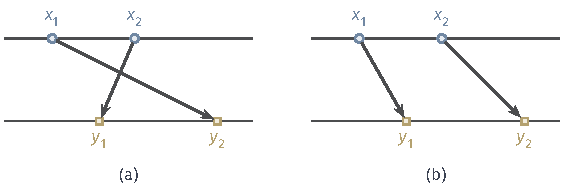
\includegraphics[width=96mm]{figures/07-probability/07-distribution-optimization/tikz/ot-uncross/figure.pdf}
 \caption{实数轴上的交换论证。上方是源点$x_1<x_2$（蓝），下方是目标点$y_1<y_2$（黄）。(a)交叉配对。(b)顺序配对。对凸成本$h(x-y)$，(b)的成本不超过(a)。}
 \label{fig:ot-uncross}
\end{BookInlineFigure}

\paragraph{分位数耦合}
设$\mu,\nu$是实数轴上的分布，分布函数为$F,G$。沿用第~\ref{chap:random-variables}章的广义分位数$F^{-1}(u)=\inf\{x:F(x)\geq u\}$，$0<u<1$，它满足
\[
 F^{-1}(u)\leq x\quad\Longleftrightarrow\quad u\leq F(x).
\]
取$U\sim\operatorname{Unif}(0,1)$，令$X=F^{-1}(U)$，$Y=G^{-1}(U)$。由上面的等价关系，$\mathbb{P}(X\leq x)=\mathbb{P}(U\leq F(x))=F(x)$，所以$X\sim\mu$；同理$Y\sim\nu$。$(X,Y)$的联合分布因此是$\mu$与$\nu$的一个耦合，称为\term{分位数耦合}（quantile coupling）。它的联合分布函数是
\begin{equation}
 \mathbb{P}(X\leq s,\ Y\leq t)=\mathbb{P}\bigl(U\leq F(s),\ U\leq G(t)\bigr)=\min\bigl(F(s),G(t)\bigr).
 \label{eq:ot-comonotone-cdf}
\end{equation}
两个分量由同一个$U$单调地决定，$U$越大两者都越大，所以这个耦合“不交叉”。

\begin{theorem}[一维最优运输]
\label{thm:ot-one-dimensional}
设$\mu,\nu$是实数轴上具有有限$p$阶矩的分布，$p\geq1$，分布函数为$F,G$，成本$c(x,y)=\lvert x-y\rvert^{p}$。则分位数耦合是最优耦合，
\begin{equation}
 W_p^{p}(\mu,\nu)=\int_0^{1}\bigl\lvert F^{-1}(u)-G^{-1}(u)\bigr\rvert^{p}\,\mathrm{d}u .
 \label{eq:ot-quantile-formula}
\end{equation}
$p=1$时还有
\begin{equation}
 W_1(\mu,\nu)=\int_{-\infty}^{\infty}\bigl\lvert F(x)-G(x)\bigr\rvert\,\mathrm{d}x .
 \label{eq:ot-cdf-formula}
\end{equation}
$p>1$时最优耦合唯一。
\end{theorem}

$p=1$与$p>1$的证明思路不同。$p=1$时成本对距离是线性的，可以把$\lvert x-y\rvert$拆成对阈值的积分，直接得到下界；$p>1$时先由第~\ref{sec:ot-existence}节取得一个最优耦合，再证明它必定不交叉，不交叉的耦合只有分位数耦合一个。

\begin{proof}[$p=1$的证明]
对实数$x,y$，示性函数$\mathbf{1}_{\{x\leq t\}}$与$\mathbf{1}_{\{y\leq t\}}$只在$t$介于$x,y$之间时不同，所以
\[
 \lvert x-y\rvert=\int_{-\infty}^{\infty}\bigl\lvert\mathbf{1}_{\{x\leq t\}}-\mathbf{1}_{\{y\leq t\}}\bigr\rvert\,\mathrm{d}t .
\]
任取耦合$(X,Y)$，两边取期望，被积函数非负，由Tonelli定理交换期望与积分，再对每个$t$用“绝对值的期望不小于期望的绝对值”，
\[
 \mathbb{E}\lvert X-Y\rvert=\int_{-\infty}^{\infty}\mathbb{E}\bigl\lvert\mathbf{1}_{\{X\leq t\}}-\mathbf{1}_{\{Y\leq t\}}\bigr\rvert\,\mathrm{d}t\geq\int_{-\infty}^{\infty}\lvert F(t)-G(t)\rvert\,\mathrm{d}t .
\]
所以式~\eqref{eq:ot-cdf-formula}右边是一切耦合成本的下界。

对分位数耦合，$\{X\leq t\}=\{U\leq F(t)\}$，$\{Y\leq t\}=\{U\leq G(t)\}$，两个事件一个包含另一个，所以
\[
 \mathbb{E}\bigl\lvert\mathbf{1}_{\{X\leq t\}}-\mathbf{1}_{\{Y\leq t\}}\bigr\rvert=\bigl\lvert F(t)-G(t)\bigr\rvert ,
\]
上面的不等式取等。分位数耦合达到下界，是最优耦合，并且$W_1$同时等于式~\eqref{eq:ot-quantile-formula}与式~\eqref{eq:ot-cdf-formula}的右边。
\end{proof}

式~\eqref{eq:ot-cdf-formula}说的是：$W_1$等于两条分布函数曲线之间的面积。式~\eqref{eq:ot-quantile-formula}说的是同一块面积换一个方向切片：按纵坐标$u$切成水平条，每条的长度是$\lvert F^{-1}(u)-G^{-1}(u)\rvert$。图~\ref{fig:ot-quantile-coupling}对全章例子画出两种看法。

$p>1$的证明需要一个关于最优耦合支撑的引理。$\mathbb{R}^{2}$上分布$\pi$的支撑是这样的点$z$的全体：以$z$为中心的每个开球都有正的$\pi$质量。支撑之外的点各有一个零质量邻域，这些邻域可以由可数个有理中心、有理半径的零质量球覆盖，所以支撑之外的总质量为零；换句话说，正质量的集合一定与支撑相交。

\begin{lemma}[最优耦合不能局部改进]
\label{lem:ot-two-point}
设$c:\mathbb{R}\times\mathbb{R}\to[0,\infty)$连续，$\pi$是$\mu,\nu$的成本有限的最优耦合。则对$\pi$支撑中的任意两点$(x_1,y_1),(x_2,y_2)$，
\begin{equation}
 c(x_1,y_1)+c(x_2,y_2)\leq c(x_1,y_2)+c(x_2,y_1).
 \label{eq:ot-two-point}
\end{equation}
\end{lemma}

\begin{proof}
设两点不同而不等式反向，差为$3\eta>0$。由连续性，可取$\delta>0$，使两个开方块
\[
 Q_k=(x_k-\delta,x_k+\delta)\times(y_k-\delta,y_k+\delta),\qquad k=1,2
\]
互不相交，并且只要$(x,y)\in Q_1$，$(x',y')\in Q_2$，就有
\[
 c(x,y)+c(x',y')\geq c(x,y')+c(x',y)+\eta .
\]
两点在支撑中，$m_k=\pi(Q_k)>0$。记$\pi_k=\pi|_{Q_k}/m_k$，它的两个边缘为$\alpha_k,\beta_k$。取$\lambda=\min(m_1,m_2)$，构造
\[
 \pi'=\pi-\lambda(\pi_1+\pi_2)+\lambda\bigl(\alpha_1\otimes\beta_2+\alpha_2\otimes\beta_1\bigr).
\]
在$Q_k$上$\pi\geq m_k\pi_k\geq\lambda\pi_k$，所以$\pi'$非负。第一边缘先减去$\lambda(\alpha_1+\alpha_2)$、再加回$\lambda(\alpha_1+\alpha_2)$，没有改变，第二边缘同理，于是$\pi'\in\Pi(\mu,\nu)$。这一步把两块中的质量“交换目的地”：$Q_1$里的源送往$Q_2$里的目标，反之亦然。成本的改变量是
\[
 \begin{aligned}
 &\lambda\iint\bigl(c(x,y')+c(x',y)-c(x,y)-c(x',y')\bigr)\,\pi_1(\mathrm{d}x,\mathrm{d}y)\,\pi_2(\mathrm{d}x',\mathrm{d}y')\\
 &\qquad\leq-\lambda\eta<0 ,
 \end{aligned}
\]
其中各项积分有限，因为$c$在有界集上有界。这与$\pi$最优矛盾。
\end{proof}

\begin{proof}[$p>1$的证明]
有限$p$阶矩保证独立耦合的成本有限，成本连续，由定理~\ref{thm:ot-existence}，最优耦合存在。任取一个最优耦合$\pi$，我们证明它就是分位数耦合，于是分位数耦合最优，而且最优耦合唯一。

\emph{第一步：支撑不交叉。}设支撑中有$(x_1,y_1),(x_2,y_2)$满足$x_1<x_2$而$y_1>y_2$。记
\[
 r=x_1-y_1,\qquad v=x_1-y_2,\qquad w=x_2-y_1,\qquad z=x_2-y_2 .
\]
则$v,w$都严格介于$r$与$z$之间，并且
\[
 v+w=r+z .
\]
令$\lambda=(z-v)/(z-r)\in(0,1)$，则
\[
 v=\lambda r+(1-\lambda)z,\qquad w=(1-\lambda)r+\lambda z .
\]
$h(s)=\lvert s\rvert^{p}$在$p>1$时严格凸，所以
\[
 h(v)+h(w)<\lambda h(r)+(1-\lambda)h(z)+(1-\lambda)h(r)+\lambda h(z)=h(r)+h(z),
\]
即$c(x_1,y_2)+c(x_2,y_1)<c(x_1,y_1)+c(x_2,y_2)$，与引理~\ref{lem:ot-two-point}矛盾。所以支撑中$x_1<x_2$蕴含$y_1\leq y_2$。

\emph{第二步：不交叉决定联合分布。}任取$s,t$。若事件$\{x\leq s,\,y>t\}$与$\{x>s,\,y\leq t\}$的$\pi$质量都为正，两者都与支撑相交，得到支撑中的点$(x_1,y_1)$、$(x_2,y_2)$，满足$x_1\leq s<x_2$且$y_2\leq t<y_1$，与第一步矛盾。所以两者至少有一个质量为零。若前者为零，
\[
 \pi(x\leq s,\,y\leq t)=\pi(x\leq s)=F(s),
\]
又因为它不超过$\pi(y\leq t)=G(t)$，它等于$\min(F(s),G(t))$。后者为零时同理。于是$\pi$的联合分布函数就是式~\eqref{eq:ot-comonotone-cdf}，二维分布由联合分布函数唯一确定，$\pi$等于分位数耦合。
\end{proof}

$p=1$时最优耦合一般不唯一。第~\ref{chap:distribution-comparison}章已经看到，例表上逐格搬运与跳格搬运的一阶成本相同；这正是$h(s)=\lvert s\rvert$不严格凸的结果，交换论证中的不等式可以取等。

\paragraph{例子的计算}
全章例子的两个分布函数与分位数函数分别是阶梯函数。$F$在$0,1,2$处跳到$0.5,0.8,1$，$G$跳到$0.2,0.5,1$。把$(0,1)$按两组跳跃高度切开，得到四个区间：
\[
 (0,0.2],\qquad(0.2,0.5],\qquad(0.5,0.8],\qquad(0.8,1).
\]
在这四段上$(F^{-1}(u),G^{-1}(u))$依次取$(0,0)$、$(0,1)$、$(1,2)$、$(2,2)$，各段长度$0.2,0.3,0.3,0.2$就是分位数耦合放在这些点对上的质量，它正是图~\ref{fig:ot-plan-tables}(c)的逐格搬运。由定理~\ref{thm:ot-one-dimensional}，逐格搬运是平方成本下唯一的最优方案，这印证了上一节用对偶势得到的结论。由式~\eqref{eq:ot-cdf-formula}，
\[
 W_1=\int_0^{1}(0.5-0.2)\,\mathrm{d}x+\int_1^{2}(0.8-0.5)\,\mathrm{d}x=0.6 ,
\]
这证明了第~\ref{chap:distribution-comparison}章提到的关系：$W_1$等于两条分布函数之间的面积。由式~\eqref{eq:ot-quantile-formula}，
\[
 W_2^{2}=0.3\times1^{2}+0.3\times1^{2}=0.6 .
\]

\begin{BookInlineFigure}
 \centering
 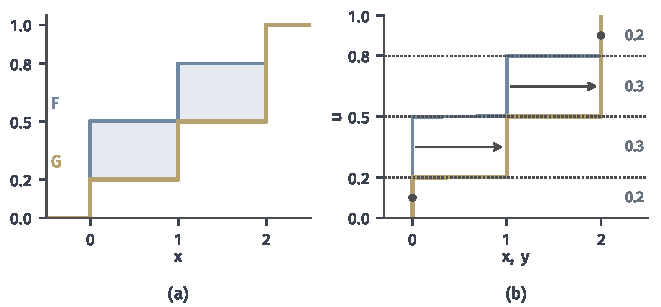
\includegraphics[width=112mm]{figures/07-probability/07-distribution-optimization/matplotlib/ot-quantile-coupling/figure.pdf}
 \caption{全章例子的一维运输。(a)$F$（蓝）与$G$（黄），两者之间浅蓝区域的面积是$W_1=0.6$。(b)分位数函数，横轴为取值，纵轴为$u$；虚线把$(0,1)$分成四段，每段内箭头从$F^{-1}(u)$指向$G^{-1}(u)$，右侧数字是该段长度，即搬运的质量；黑点表示质量留在原地。}
 \label{fig:ot-quantile-coupling}
\end{BookInlineFigure}

\paragraph{何时由映射实现}
分位数耦合是$U$的函数对，但不一定是$X$的函数。若$F$连续，它是。先说明$F(X)\sim\operatorname{Unif}(0,1)$：由分位数的等价关系，$F(x)\geq u$当且仅当$x\geq F^{-1}(u)$，而$F$连续时$\mathbb{P}(X=F^{-1}(u))=0$且$F(F^{-1}(u))=u$，所以
\[
 \mathbb{P}\bigl(F(X)\geq u\bigr)=\mathbb{P}\bigl(X\geq F^{-1}(u)\bigr)=1-u .
\]
再说明$F^{-1}(F(X))=X$几乎必然成立：总有$F^{-1}(F(x))\leq x$，严格小于只发生在$F$的平台上，平台的质量为零。于是取$U=F(X)$，分位数耦合就是$(X,\,G^{-1}(F(X)))$，
\begin{equation}
 T=G^{-1}\circ F
 \label{eq:ot-monotone-map}
\end{equation}
是一个单调不减的最优运输映射。

源分布有原子时，分位数耦合必须把原子拆开。取
\[
 \mu=\tfrac12\delta_0+\tfrac12\operatorname{Unif}(1,2),\qquad \nu=\operatorname{Unif}(0,2),
\]
则
\[
 F^{-1}(u)=\begin{cases}0, & u\leq\tfrac12,\\ 2u, & u>\tfrac12,\end{cases}\qquad G^{-1}(u)=2u .
\]
$u\leq\tfrac12$时，$0$处的原子被均匀地铺到$[0,1]$上；$u>\tfrac12$时质量不动。由式~\eqref{eq:ot-quantile-formula}，
\[
 W_1=\int_0^{1/2}2u\,\mathrm{d}u=\frac14,\qquad W_2^{2}=\int_0^{1/2}4u^{2}\,\mathrm{d}u=\frac16 .
\]
$W_1$也等于图~\ref{fig:ot-atom-quantile}(a)中$F$与$G$之间三角形的面积$\tfrac12\times1\times\tfrac12$。这里不存在任何运输映射：映射把$0$处质量为$\tfrac12$的原子整体送到一个点，像分布就有质量至少$\tfrac12$的原子，而$\nu$没有原子。分位数配对总能定义耦合，却未必给出源点的单值映射。

\begin{BookInlineFigure}
 \centering
 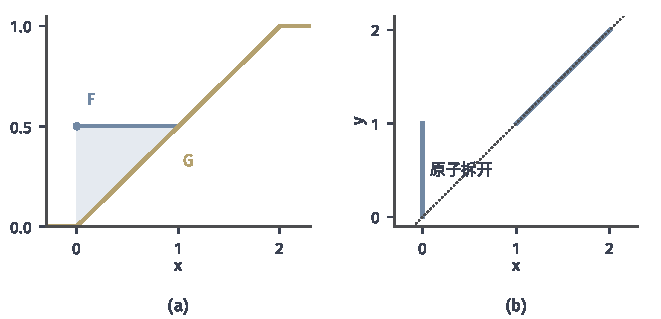
\includegraphics[width=112mm]{figures/07-probability/07-distribution-optimization/matplotlib/ot-atom-quantile/figure.pdf}
 \caption{带原子的源分布$\mu=\tfrac12\delta_0+\tfrac12\operatorname{Unif}(1,2)$与$\nu=\operatorname{Unif}(0,2)$。(a)$F$（蓝）与$G$（黄），在$[1,2]$上两者重合；浅蓝三角形面积$W_1=1/4$。(b)分位数耦合的支撑：$x=0$处的竖线表示原子被铺到$[0,1]$上，$[1,2]$上的斜线表示质量不动。}
 \label{fig:ot-atom-quantile}
\end{BookInlineFigure}

\subsection{离散运输}
\label{sec:ot-discrete}

高维的有限问题没有顺序可用，只能直接解线性规划。把$\bm{\pi}$排成长为$mn$的向量，问题是$m+n$个等式约束、$mn$个非负变量的线性规划。行约束之和与列约束之和都等于总质量$1$，所以等式约束中有一个是多余的，独立的约束是$m+n-1$个。

\paragraph{顶点的结构}
由前面提到的线性规划理论，线性规划若有最优解，就有一个最优解是可行集合的顶点。运输多面体的顶点有简单的组合刻画。把$\bm{\pi}$的非零位置看成二部图的边：左边是源点，右边是目标点，$\pi_{i,j}>0$时连接$i$与$j$。若这些边含有一个圈$i_1\to j_1\to i_2\to j_2\to\cdots\to i_1$，沿圈交替地对各边加上和减去一个小量$\epsilon$，每个点上一加一减，行和列和不变。于是$\bm{\pi}$是两个可行方案$\bm{\pi}\pm\epsilon\bm{D}$的中点，不是顶点。所以顶点的非零位置不含圈，构成一个森林，边数至多是点数减一，即
\[
 \#\{(i,j):\pi_{i,j}>0\}\leq m+n-1 .
\]
最优顶点因此很稀疏，但稀疏不等于一一配对：$m\neq n$时一一配对根本不可能，$m=n$时一个源点也可能把质量分给几个目标点。

当$m=n$且$\bm{a}=\bm{b}=\tfrac1n\bm{1}$时，顶点恰好是置换矩阵除以$n$。森林中总有只连一条边的点，比如第$i$行只有一个非零元$\pi_{i,j}$，它必须等于行和$\tfrac1n$，于是第$j$列也已满额；删去这一行一列，剩下的仍是同类问题，归纳下去即得。这时最优运输就是\term{指派问题}（assignment problem），可参考\BookChapterRef{chap:bipartite-matching-assignment}{卷三第6章“二部图匹配与指派”}。

\paragraph{网络流的视角}
运输问题也是一个最小费用流问题：从每个源点$i$流出$a_i$，流入每个目标点$j$恰好$b_j$，弧$(i,j)$上单位流量的费用是$c_{i,j}$，没有容量上限。网络单纯形法在可行生成树之间移动，正是在运输多面体的顶点之间移动；它维护的节点势就是本章的对偶势，判断最优的“没有负费用圈”等价于所有松弛量非负。这些方法可参考\BookChapterRef{chap:min-cost-flow}{卷三第7章“最小费用流”}。

\paragraph{平面上的例子}
取平面上的三个源点与四个目标点，成本为平方欧氏距离：
\[
 \begin{aligned}
 &x_1=(0,0),\quad x_2=(0,2),\quad x_3=(3,1),\\
 &\bm{a}=(0.4,\ 0.4,\ 0.2),\\
 &y_1=(1,0),\quad y_2=(2,2),\quad y_3=(4,0),\quad y_4=(1,3),\\
 &\bm{b}=(0.3,\ 0.3,\ 0.2,\ 0.2).
 \end{aligned}
\]
成本矩阵与一个最优方案是
\[
 \bm{C}=\begin{bmatrix}1&8&16&10\\5&4&20&2\\5&2&2&8\end{bmatrix},\qquad
 \bm{\pi}^{*}=\begin{bmatrix}0.3&0.1&0&0\\0&0.2&0&0.2\\0&0&0.2&0\end{bmatrix},
\]
成本是
\[
 0.3\times1+0.1\times8+0.2\times4+0.2\times2+0.2\times2=2.7 .
\]
图~\ref{fig:ot-lp-plane}画出这个方案。$x_1$的质量分给了$y_1$与$y_2$，$y_2$从两个源点收货；非零元有$5$个，少于$m+n-1=6$，是一个退化的顶点。

\begin{BookInlineFigure}
 \centering
 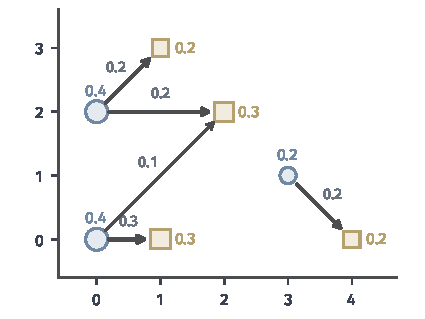
\includegraphics[width=72mm]{figures/07-probability/07-distribution-optimization/matplotlib/ot-lp-plane/figure.pdf}
 \caption{平面上的离散运输，平方欧氏成本。蓝圆是源点，黄方块是目标点，旁边的数是质量；箭头是最优方案的非零元，粗细与箭头旁的数表示搬运的质量。最优成本为$2.7$。}
 \label{fig:ot-lp-plane}
\end{BookInlineFigure}

\paragraph{结果的检验}
线性规划求解器输出的方案要逐项检验，不能只看目标值。检验三件事。第一，非负性：$\min_{i,j}\pi_{i,j}\geq0$。第二，边缘残差：行和与$\bm{a}$之差、列和与$\bm{b}$之差的$\ell_1$范数之和应为零，数值解应在容差以内；不满足边缘约束的方案，其成本不是最优值的上界。第三，原对偶差：再给出一对势$(\bm{f},\bm{g})$，检查对偶可行性$\max_{i,j}(f_i+g_j-c_{i,j})\leq0$，并计算$\langle\bm{C},\bm{\pi}\rangle-\langle\bm{a},\bm{f}\rangle-\langle\bm{b},\bm{g}\rangle$。由式~\eqref{eq:ot-gap}，前两项满足时这个差非负并且控制方案与最优值的距离。

对上面的例子，令$f_1=0$，在非零位置上解$f_i+g_j=c_{i,j}$，得$g_1=1$，$g_2=8$，$f_2=-4$，$g_4=6$；第三个源点只连$y_3$，自成一棵树，$f_3+g_3=2$还有一个自由度，取$f_3=-6$，$g_3=8$。于是
\[
 \bm{f}=(0,\ -4,\ -6),\qquad \bm{g}=(1,\ 8,\ 8,\ 6),
\]
松弛矩阵是
\[
 \bm{C}-\bigl(f_i+g_j\bigr)_{i,j}=\begin{bmatrix}0&0&8&4\\8&0&16&0\\10&0&0&8\end{bmatrix}\geq0 ,
\]
对偶值是
\[
 \langle\bm{a},\bm{f}\rangle+\langle\bm{b},\bm{g}\rangle=-2.8+5.5=2.7 ,
\]
原对偶差为零，$\bm{\pi}^{*}$最优。它也是唯一的最优方案：零松弛位置只有$(1,1),(1,2),(2,2),(2,4),(3,2),(3,3)$，第三列只有$(3,3)$一处零松弛，所以第三个源点的$0.2$必须全部给$y_3$，$(3,2)$只能为零；其余位置随之唯一确定。

\subsection{高斯分布的二次运输}
\label{sec:ot-gaussian}

在$\mathbb{R}^{d}$上取平方欧氏成本，$c(x,y)=\lVert x-y\rVert_2^{2}$。先把均值分离出去。设$X\sim\mu$，$Y\sim\nu$，均值分别是$\bm{m}_1,\bm{m}_2$，二阶矩有限，记$\tilde{X}=X-\bm{m}_1$，$\tilde{Y}=Y-\bm{m}_2$。对任意耦合，
\[
 \mathbb{E}\lVert X-Y\rVert_2^{2}=\lVert\bm{m}_1-\bm{m}_2\rVert_2^{2}+2\bigl\langle\bm{m}_1-\bm{m}_2,\ \mathbb{E}[\tilde{X}-\tilde{Y}]\bigr\rangle+\mathbb{E}\lVert\tilde{X}-\tilde{Y}\rVert_2^{2},
\]
中间项为零。所以平方运输成本等于均值之差的平方加上把两个中心化分布对齐的成本，两部分互不影响。中心化部分再展开，
\[
 \mathbb{E}\lVert\tilde{X}-\tilde{Y}\rVert_2^{2}=\operatorname{tr}\bm{\Sigma}_1+\operatorname{tr}\bm{\Sigma}_2-2\,\mathbb{E}\langle\tilde{X},\tilde{Y}\rangle ,
\]
其中$\bm{\Sigma}_1,\bm{\Sigma}_2$是协方差矩阵。前两项只依赖边缘，所以最小化成本就是最大化$\mathbb{E}\langle\tilde{X},\tilde{Y}\rangle$：让两个向量尽可能“同向”。

\begin{theorem}[高斯分布的平方运输]
\label{thm:ot-gaussian}
设$\mu=\mathcal{N}(\bm{m}_1,\bm{\Sigma}_1)$，$\nu=\mathcal{N}(\bm{m}_2,\bm{\Sigma}_2)$，两个协方差矩阵都正定。令
\begin{equation}
 \bm{A}=\bm{\Sigma}_1^{-1/2}\bigl(\bm{\Sigma}_1^{1/2}\bm{\Sigma}_2\bm{\Sigma}_1^{1/2}\bigr)^{1/2}\bm{\Sigma}_1^{-1/2},\qquad T(x)=\bm{m}_2+\bm{A}(x-\bm{m}_1).
 \label{eq:ot-gaussian-map}
\end{equation}
则$T$是从$\mu$到$\nu$的最优运输映射，并且
\begin{equation}
 W_2^{2}(\mu,\nu)=\lVert\bm{m}_1-\bm{m}_2\rVert_2^{2}+\operatorname{tr}\bm{\Sigma}_1+\operatorname{tr}\bm{\Sigma}_2-2\operatorname{tr}\bigl(\bm{\Sigma}_1^{1/2}\bm{\Sigma}_2\bm{\Sigma}_1^{1/2}\bigr)^{1/2}.
 \label{eq:ot-gaussian-w2}
\end{equation}
\end{theorem}

这里的平方根都是对称正定矩阵的唯一对称正定平方根。记$\bm{M}$为式~\eqref{eq:ot-gaussian-map}中括号的平方根，它对称正定；$\bm{A}$是对称正定矩阵与它的合同变换，仍对称正定。

\begin{proof}
\emph{映射可行。}$T$是仿射映射，$T(X)$是高斯向量，均值为$\bm{m}_2$，协方差为
\[
 \bm{A}\bm{\Sigma}_1\bm{A}=\bm{\Sigma}_1^{-1/2}\bm{M}\bm{\Sigma}_1^{-1/2}\bm{\Sigma}_1\bm{\Sigma}_1^{-1/2}\bm{M}\bm{\Sigma}_1^{-1/2}=\bm{\Sigma}_1^{-1/2}\bm{M}^{2}\bm{\Sigma}_1^{-1/2}=\bm{\Sigma}_2 .
\]
所以$T_\#\mu=\nu$。

\emph{映射最优。}由前面的分解，只需证明对中心化的任意耦合$(\tilde{X},\tilde{Y})$，内积的期望$\mathbb{E}\langle\tilde{X},\tilde{Y}\rangle$不超过$\tilde{Y}=\bm{A}\tilde{X}$时的值。对任意向量$x,y$，
\[
 \tfrac12\langle x,\bm{A}x\rangle+\tfrac12\langle y,\bm{A}^{-1}y\rangle-\langle x,y\rangle=\tfrac12\bigl\lVert\bm{A}^{1/2}x-\bm{A}^{-1/2}y\bigr\rVert_2^{2}\geq0 ,
\]
等号当且仅当$y=\bm{A}x$。代入$x=\tilde{X}$，$y=\tilde{Y}$并取期望，
\[
 \mathbb{E}\langle\tilde{X},\tilde{Y}\rangle\leq\tfrac12\operatorname{tr}(\bm{A}\bm{\Sigma}_1)+\tfrac12\operatorname{tr}(\bm{A}^{-1}\bm{\Sigma}_2).
\]
右边只依赖两个边缘，是一切耦合的公共上界；$\tilde{Y}=\bm{A}\tilde{X}$时取等，而这正是$T$给出的耦合。

\emph{成本。}在$T$给出的耦合下，$\mathbb{E}\langle\tilde{X},\bm{A}\tilde{X}\rangle$等于$\operatorname{tr}(\bm{A}\bm{\Sigma}_1)$，并且
\[
 \operatorname{tr}(\bm{A}\bm{\Sigma}_1)=\operatorname{tr}\bigl(\bm{\Sigma}_1^{-1/2}\bm{M}\bm{\Sigma}_1^{1/2}\bigr)=\operatorname{tr}\bm{M} .
\]
代入前面的分解即得式~\eqref{eq:ot-gaussian-w2}。
\end{proof}

证明中的二次型不等式是凸函数$\tfrac12\langle x,\bm{A}x\rangle$与它的凸共轭之间的Fenchel--Young不等式。一般地，平方成本下的最优映射是某个凸函数的梯度，这里的凸函数是二次函数，梯度就是对称正定的线性映射$\bm{A}$。对称性是关键：同样把$\mu$推成$\nu$的映射还有许多，但只有对称正定的那一个是最优的。

一维时式~\eqref{eq:ot-gaussian-w2}化为
\begin{equation}
 W_2^{2}\bigl(\mathcal{N}(m_1,\sigma_1^{2}),\mathcal{N}(m_2,\sigma_2^{2})\bigr)=(m_1-m_2)^{2}+(\sigma_1-\sigma_2)^{2},
 \label{eq:ot-gaussian-1d}
\end{equation}
最优映射是$T(x)=m_2+(\sigma_2/\sigma_1)(x-m_1)$，也就是第~\ref{sec:ot-one-dimensional}节的$G^{-1}\circ F$。

\paragraph{一个能手算的例子}
取$\mu=\mathcal{N}(\bm{0},\bm{I})$，$\nu=\mathcal{N}(\bm{m},\bm{\Sigma}_2)$，其中
\[
 \bm{m}=(3,\ 1),\qquad \bm{\Sigma}_2=\operatorname{diag}\bigl(4,\ \tfrac14\bigr).
\]
$\bm{\Sigma}_1=\bm{I}$，所以$\bm{A}=\bm{M}=\bm{\Sigma}_2^{1/2}$，即$\operatorname{diag}(2,\tfrac12)$，最优映射是
\[
 T(x)=(3,\ 1)+\bigl(2x_1,\ \tfrac12x_2\bigr).
\]
由式~\eqref{eq:ot-gaussian-w2}，
\[
 W_2^{2}=10+2+\tfrac{17}{4}-2\bigl(2+\tfrac12\bigr)=10+1.25=11.25 ,
\]
均值移动贡献$10$，形状改变贡献$(1-2)^{2}+(1-\tfrac12)^{2}=1.25$。

作为对照，先把$x$旋转$90^{\circ}$再拉伸：
\[
 T'(x)=\bm{m}+\operatorname{diag}\bigl(2,\tfrac12\bigr)\bm{R}x,\qquad \bm{R}=\begin{bmatrix}0&-1\\1&0\end{bmatrix}.
\]$\bm{R}\bm{R}^{\top}=\bm{I}$，所以$T'(X)$的协方差仍是$\bm{\Sigma}_2$，$T'$也是运输映射。它的成本是
\[
 10+\operatorname{tr}\bm{I}+\operatorname{tr}\bm{\Sigma}_2-2\operatorname{tr}\bigl(\operatorname{diag}(2,\tfrac12)\bm{R}\bigr)=10+2+4.25-0=16.25 .
\]
$\operatorname{diag}(2,\tfrac12)\bm{R}$不对称，对角线为零，它让$\tilde{X}$与$\tilde{Y}$完全不同向。图~\ref{fig:ot-gaussian-map}对比了两个映射：红点$(1,0)$在最优映射下送到$(5,1)$，在$T'$下送到$(3,\tfrac32)$。

\begin{BookInlineFigure}
 \centering
 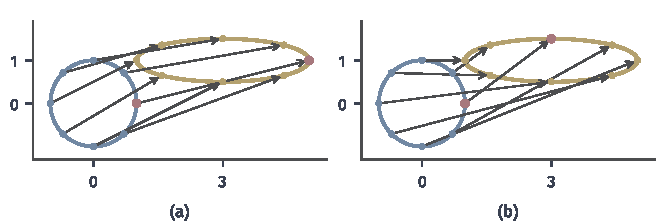
\includegraphics[width=112mm]{figures/07-probability/07-distribution-optimization/matplotlib/ot-gaussian-map/figure.pdf}
 \caption{$\mathcal{N}(\bm{0},\bm{I})$（蓝圈为单位标准差等高线）到$\mathcal{N}((3,1),\operatorname{diag}(4,\tfrac14))$（黄椭圆）。箭头是圆上八个点的像，红点是$(1,0)$及其像。(a)最优映射$T(x)=\bm{m}+\operatorname{diag}(2,\tfrac12)x$，成本$11.25$。(b)先旋转$90^{\circ}$再拉伸的映射，像分布相同，成本$16.25$。}
 \label{fig:ot-gaussian-map}
\end{BookInlineFigure}

\paragraph{奇异协方差}
定理要求$\bm{\Sigma}_1$可逆，因为$\bm{A}$的公式含$\bm{\Sigma}_1^{-1/2}$。源分布退化时，最优耦合与最优成本仍可研究，但必须按支撑子空间检查映射是否可行。取$d=2$，
\[
 \mu=\mathcal{N}\bigl(\bm{0},\operatorname{diag}(1,0)\bigr),\qquad \nu=\mathcal{N}(\bm{0},\bm{I}).
\]
$\mu$集中在横轴上，$X=(X_1,0)$。两者均值都是零，由前面的分解，最小化成本就是最大化$\mathbb{E}\langle X,Y\rangle$。对任意耦合，由Cauchy--Schwarz不等式，
\[
 \mathbb{E}\langle X,Y\rangle=\mathbb{E}[X_1Y_1]\leq\sqrt{\mathbb{E}X_1^{2}\,\mathbb{E}Y_1^{2}}=1 ,
\]
等号当且仅当$Y_1=X_1$。于是最优耦合必须让$Y_1=X_1$，而$Y_2$要服从$\mathcal{N}(0,1)$并且与$Y_1$独立（$\nu$的两个分量独立），所以最优耦合唯一：
\[
 Y=(X_1,\ Z),\qquad Z\sim\mathcal{N}(0,1)\ \text{与}\ X_1\ \text{独立},
\]
成本是$\mathbb{E}Z^{2}=1$。$Y_2$与$X$独立，不是$X$的函数，所以最优耦合不由映射产生，见图~\ref{fig:ot-gaussian-singular}。

反方向的问题落在定理~\ref{thm:ot-gaussian}之内。把两个分布对调，以$\nu$为源，它的协方差可逆，式~\eqref{eq:ot-gaussian-w2}给出
\[
 0+2+1-2\operatorname{tr}\operatorname{diag}(1,0)=1 ,
\]
与直接计算一致；对调方向的最优映射是投影$(y_1,y_2)\mapsto(y_1,0)$。协方差奇异时式~\eqref{eq:ot-gaussian-w2}本身仍然成立，可以用正定情形取极限得到，但不能把含$\bm{\Sigma}_1^{-1/2}$的映射公式直接套用。

\begin{BookInlineFigure}
 \centering
 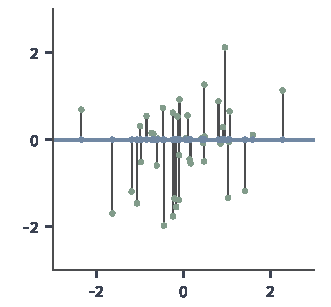
\includegraphics[width=56mm]{figures/07-probability/07-distribution-optimization/matplotlib/ot-gaussian-singular/figure.pdf}
 \caption{退化源分布$\mathcal{N}(\bm{0},\operatorname{diag}(1,0))$（蓝线为其支撑）到$\mathcal{N}(\bm{0},\bm{I})$的唯一最优耦合，$40$对模拟点，种子$729$。蓝点是源点，绿点是目标点，竖线是搬运路径：每份质量只沿竖直方向移动，目标高度与源点独立。}
 \label{fig:ot-gaussian-singular}
\end{BookInlineFigure}

\section{熵正则化}
\label{sec:ot-entropic}

$m$个源点、$n$个目标点的运输线性规划有$mn$个变量。分布由细网格离散化时，$m,n$成千上万，单纯形类方法要在巨大的多面体顶点之间移动，而且最优解落在边界上，对数据的微小变化不连续。一个常用的办法是在成本上加一个惩罚，鼓励方案“散开”一些：散开的方案位于多面体内部，最优性条件变成光滑的方程，可以用简单的交替缩放求解。代价是求得的不再是原问题的最优方案。本节研究这一权衡。

\paragraph{正则化问题}
设$\bm{a}\in\mathbb{R}^{m}$，$\bm{b}\in\mathbb{R}^{n}$是概率向量。若某个$a_i=0$，任何可行方案的第$i$行都必须为零，这一行可以直接删去；对$b_j=0$的列也一样。所以下面总设$\bm{a},\bm{b}$的各分量都为正。以边缘乘积$\bm{a}\otimes\bm{b}$，即独立方案$(a_ib_j)_{i,j}$为参考，对$\varepsilon>0$考虑
\begin{equation}
 \min_{\bm{\pi}\in U(\bm{a},\bm{b})}\ L_\varepsilon(\bm{\pi}),\qquad L_\varepsilon(\bm{\pi})=\langle\bm{C},\bm{\pi}\rangle+\varepsilon D_{\mathrm{KL}}(\bm{\pi}\Vert\bm{a}\otimes\bm{b}),
 \label{eq:ot-entropic-problem}
\end{equation}
其中
\[
 D_{\mathrm{KL}}(\bm{\pi}\Vert\bm{a}\otimes\bm{b})=\sum_{i,j}\pi_{i,j}\ln\frac{\pi_{i,j}}{a_ib_j},
\]
约定$0\ln0=0$。这一问题称为\term{熵正则化最优运输}（entropic optimal transport）。

两项各有含义。$\langle\bm{C},\bm{\pi}\rangle$是原来的运输成本；KL项是方案偏离独立方案的程度。把$\bm{\pi}$看成$(X,Y)$的联合分布，它的两个边缘是$\bm{a},\bm{b}$，所以这一项正是第~\ref{chap:information-measures}章的互信息$I(X;Y)$：它衡量知道源位置后，对目标位置的不确定性减少了多少。$\varepsilon$很大时，惩罚迫使方案接近独立方案，源与目标几乎无关；$\varepsilon\to0$时，方案回到原问题的最优方案，源几乎决定目标。图~\ref{fig:ot-entropic-plans}在一个细网格上展示这一变化。

\begin{BookInlineFigure}
 \centering
 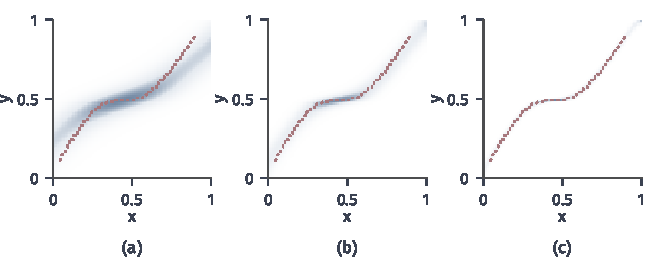
\includegraphics[width=112mm]{figures/07-probability/07-distribution-optimization/matplotlib/ot-entropic-plans/figure.pdf}
 \caption{$[0,1]$上$80$个格点的熵正则化方案，源为双峰分布，目标为单峰分布，平方成本。图中是按行归一化后的方案，即给定$x$时$y$的条件分布，颜色越深概率越大；红色点线是不加正则化时的单调最优映射。(a)$\varepsilon=0.02$。(b)$\varepsilon=0.005$。(c)$\varepsilon=0.0005$。}
 \label{fig:ot-entropic-plans}
\end{BookInlineFigure}

\paragraph{对偶问题与原对偶差}
正则化问题的对偶变量仍是一对向量$\bm{f}\in\mathbb{R}^{m}$，$\bm{g}\in\mathbb{R}^{n}$，但约束$f_i+g_j\leq c_{i,j}$换成一个光滑的惩罚：
\begin{equation}
 D_\varepsilon(\bm{f},\bm{g})=\langle\bm{a},\bm{f}\rangle+\langle\bm{b},\bm{g}\rangle-\varepsilon\sum_{i,j}a_ib_j\Bigl(\mathrm{e}^{(f_i+g_j-c_{i,j})/\varepsilon}-1\Bigr).
 \label{eq:ot-entropic-dual}
\end{equation}
违反约束越多，指数项越大；$\varepsilon\to0$时，它趋于“满足约束为$0$、违反约束为$-\infty$”的硬约束。下面的引理是第~\ref{sec:ot-potentials}节式~\eqref{eq:ot-gap}的对应物。

\begin{lemma}[正则化问题的原对偶差]
\label{lem:ot-entropic-gap}
对$\bm{\pi}\in U(\bm{a},\bm{b})$与任意$\bm{f},\bm{g}$，记$r_{i,j}=\pi_{i,j}/(a_ib_j)$，$s_{i,j}=(f_i+g_j-c_{i,j})/\varepsilon$。则
\begin{equation}
 L_\varepsilon(\bm{\pi})-D_\varepsilon(\bm{f},\bm{g})=\varepsilon\sum_{i,j}a_ib_j\bigl(r_{i,j}\ln r_{i,j}-r_{i,j}-r_{i,j}s_{i,j}+\mathrm{e}^{s_{i,j}}\bigr)\geq0 ,
 \label{eq:ot-entropic-gap}
\end{equation}
每一项取等当且仅当$r_{i,j}=\mathrm{e}^{s_{i,j}}$。
\end{lemma}

\begin{proof}
由行列约束，
\[
 \langle\bm{a},\bm{f}\rangle+\langle\bm{b},\bm{g}\rangle=\sum_{i,j}\pi_{i,j}(f_i+g_j);
\]
又$\bm{a}\otimes\bm{b}$与$\bm{\pi}$的元素总和都是$1$。代入式~\eqref{eq:ot-entropic-dual}，
\[
 L_\varepsilon(\bm{\pi})-D_\varepsilon(\bm{f},\bm{g})=\sum_{i,j}\pi_{i,j}(c_{i,j}-f_i-g_j)+\varepsilon\sum_{i,j}\pi_{i,j}\ln r_{i,j}+\varepsilon\sum_{i,j}a_ib_j\mathrm{e}^{s_{i,j}}-\varepsilon .
\]
把$\pi_{i,j}(c_{i,j}-f_i-g_j)$写成$-\varepsilon a_ib_jr_{i,j}s_{i,j}$，把常数$\varepsilon$写成$\varepsilon\sum_{i,j}a_ib_jr_{i,j}$，即得等式。

对固定的$r\geq0$，函数$s\mapsto\mathrm{e}^{s}-rs$在$r>0$时于$s=\ln r$处取最小值$r-r\ln r$，所以
\[
 r\ln r-r-rs+\mathrm{e}^{s}\geq r\ln r-r+r-r\ln r=0 ,
\]
等号当且仅当$s=\ln r$；$r=0$时这一项是$\mathrm{e}^{s}>0$。
\end{proof}

\begin{theorem}[熵正则化问题的解]
\label{thm:ot-entropic-solution}
设$\bm{a},\bm{b}$各分量为正，$\bm{C}$各元素有限，$\varepsilon>0$。则问题~\eqref{eq:ot-entropic-problem}有唯一解$\bm{\pi}^{\varepsilon}$，它的各元素都为正，并且存在$\bm{f},\bm{g}$使
\begin{equation}
 \pi^{\varepsilon}_{i,j}=a_ib_j\,\mathrm{e}^{(f_i+g_j-c_{i,j})/\varepsilon}.
 \label{eq:ot-entropic-form}
\end{equation}
这样的$(\bm{f},\bm{g})$使$D_\varepsilon$取最大值，并且最大值等于$L_\varepsilon(\bm{\pi}^{\varepsilon})$。反过来，$U(\bm{a},\bm{b})$中任何形如式~\eqref{eq:ot-entropic-form}的方案都是唯一解。
\end{theorem}

\begin{proof}
\emph{存在与唯一。}$t\mapsto t\ln t$在$[0,\infty)$上连续，所以$L_\varepsilon$在紧集$U(\bm{a},\bm{b})$上连续，最小值取得。$t\mapsto t\ln(t/(a_ib_j))$严格凸，成本项是线性的，所以$L_\varepsilon$在凸集$U(\bm{a},\bm{b})$上严格凸，最小点唯一。

\emph{各元素为正。}设可行的$\bm{\pi}$有零元素。对$0<\lambda<1$令
\[
 \bm{\pi}^{\lambda}=(1-\lambda)\bm{\pi}+\lambda\,\bm{a}\otimes\bm{b},
\]
它是两个可行方案的凸组合，仍可行。成本项与$\bm{\pi}$的正元素对应的熵项都是$\lambda$的可微函数，它们的变化不超过$K\lambda$（$K$为常数，$\lambda$足够小）。$\bm{\pi}$的零元素$(i,j)$处，熵项从$0$变为
\[
 \lambda a_ib_j\ln\frac{\lambda a_ib_j}{a_ib_j}=\lambda a_ib_j\ln\lambda .
\]
记$\kappa>0$为零元素处$a_ib_j$之和，则
\[
 L_\varepsilon(\bm{\pi}^{\lambda})-L_\varepsilon(\bm{\pi})\leq\lambda\bigl(K+\varepsilon\kappa\ln\lambda\bigr),
\]
$\lambda$足够小时右边为负。所以有零元素的方案不是最小点。

\emph{缩放形式。}最小点$\bm{\pi}^{\varepsilon}$各元素为正，对任何行和、列和都为零的矩阵$\bm{D}$，$\bm{\pi}^{\varepsilon}+t\bm{D}$在$\lvert t\rvert$很小时可行。$t\mapsto L_\varepsilon(\bm{\pi}^{\varepsilon}+t\bm{D})$在$t=0$处取最小，导数为零：
\[
 \sum_{i,j}D_{i,j}h_{i,j}=0,\qquad h_{i,j}=c_{i,j}+\varepsilon\ln\frac{\pi^{\varepsilon}_{i,j}}{a_ib_j}+\varepsilon .
\]
对$i<m$，$j<n$取$\bm{D}$在$(i,j),(m,n)$处为$1$、在$(i,n),(m,j)$处为$-1$、其余为$0$，它的行和、列和都是零，代入得
\[
 h_{i,j}=(h_{i,n}-h_{m,n})+h_{m,j} .
\]
令$\alpha_i=h_{i,n}-h_{m,n}$，$\beta_j=h_{m,j}$，可以逐一核对$h_{i,j}=\alpha_i+\beta_j$对包括末行末列在内的一切$i,j$成立。取$f_i=\alpha_i-\varepsilon$，$g_j=\beta_j$，解出$\pi^{\varepsilon}_{i,j}$即得式~\eqref{eq:ot-entropic-form}。

\emph{对偶。}式~\eqref{eq:ot-entropic-form}说的就是$r_{i,j}=\mathrm{e}^{s_{i,j}}$，由引理~\ref{lem:ot-entropic-gap}，原对偶差为零。对任何$(\bm{f}',\bm{g}')$，同一引理说明它的对偶值不超过$L_\varepsilon(\bm{\pi}^{\varepsilon})$，而$(\bm{f},\bm{g})$的对偶值等于它，所以$(\bm{f},\bm{g})$使$D_\varepsilon$最大。反过来，可行且形如式~\eqref{eq:ot-entropic-form}的方案使原对偶差为零，它的$L_\varepsilon$值等于一个下界，是最小点。
\end{proof}

记$u_i=\mathrm{e}^{f_i/\varepsilon}$，$v_j=\mathrm{e}^{g_j/\varepsilon}$，以及正矩阵
\begin{equation}
 K_{i,j}=a_ib_j\,\mathrm{e}^{-c_{i,j}/\varepsilon},
 \label{eq:ot-gibbs-kernel}
\end{equation}
式~\eqref{eq:ot-entropic-form}写成
\begin{equation}
 \bm{\pi}^{\varepsilon}=\operatorname{diag}(\bm{u})\,\bm{K}\operatorname{diag}(\bm{v}).
 \label{eq:ot-scaling-form}
\end{equation}正则化解是固定矩阵$\bm{K}$的行与列分别乘上一个正因子。问题于是变成：找正向量$\bm{u},\bm{v}$，使缩放后的矩阵行和为$\bm{a}$、列和为$\bm{b}$。

\paragraph{正则化目标与运输成本}
正则化问题的解给出两个数：正则化目标值$L_\varepsilon(\bm{\pi}^{\varepsilon})$，以及它的运输成本$\langle\bm{C},\bm{\pi}^{\varepsilon}\rangle$。两者都不等于原问题的最优值$\operatorname{OT}$，必须分开记录。设$\bm{\pi}^{*}$是原问题的一个最优方案。$\bm{\pi}^{\varepsilon}$使$L_\varepsilon$最小，所以它的$L_\varepsilon$值不超过$\bm{\pi}^{*}$的值；再利用KL非负，
\begin{equation}
 0\leq\langle\bm{C},\bm{\pi}^{\varepsilon}\rangle-\operatorname{OT}\leq\varepsilon D_{\mathrm{KL}}(\bm{\pi}^{*}\Vert\bm{a}\otimes\bm{b})\leq\varepsilon\min\bigl(H(\bm{a}),H(\bm{b})\bigr),
 \label{eq:ot-entropic-bias}
\end{equation}
熵以奈特计。左边的不等式是因为$\bm{\pi}^{\varepsilon}$可行；最后一步是因为互信息不超过任一边缘的熵（第~\ref{chap:information-measures}章）。所以运输成本的偏差随$\varepsilon$线性地趋于零。

全章例子中，$\bm{\pi}^{*}$是逐格搬运，
\[
 \begin{aligned}
 D_{\mathrm{KL}}(\bm{\pi}^{*}\Vert\bm{a}\otimes\bm{b})&=2\times0.2\ln\frac{0.2}{0.1}+2\times0.3\ln\frac{0.3}{0.15}\\
 &=\ln2\approx0.693 .
 \end{aligned}
\]
$\varepsilon=1$时数值求得$\langle\bm{C},\bm{\pi}^{\varepsilon}\rangle\approx0.814$，偏差$0.214$，在上界$0.693$之内；正则化目标值约为$1.087$，比运输成本还多出$\varepsilon D_{\mathrm{KL}}(\bm{\pi}^{\varepsilon}\Vert\bm{a}\otimes\bm{b})\approx0.272$。图~\ref{fig:ot-entropic-bias}画出两者随$\varepsilon$的变化：$\varepsilon\to\infty$时运输成本趋于独立方案的$1.58$，$\varepsilon\to0$时趋于$0.6$。

\begin{BookInlineFigure}
 \centering
 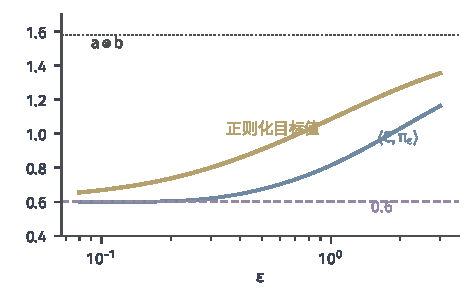
\includegraphics[width=80mm]{figures/07-probability/07-distribution-optimization/matplotlib/ot-entropic-bias/figure.pdf}
 \caption{全章例子的熵正则化偏差，横轴为$\varepsilon$（对数刻度）。蓝线是正则化解的运输成本$\langle\bm{C},\bm{\pi}^{\varepsilon}\rangle$，黄线是正则化目标值$L_\varepsilon(\bm{\pi}^{\varepsilon})$，紫色虚线是原问题最优值$0.6$，深灰点线是独立方案的成本$1.58$。}
 \label{fig:ot-entropic-bias}
\end{BookInlineFigure}

\subsection{Sinkhorn迭代}
\label{sec:ot-sinkhorn}

要找的是两个缩放向量。若列因子$\bm{v}$已知，行条件$\sum_ju_iK_{i,j}v_j=a_i$对每个$i$只含一个未知数$u_i$，立即解出；反过来，行因子已知时列因子也立即解出。于是交替地做这两件事。

\paragraph{交替缩放}
固定$\bm{v}$，令行和等于$\bm{a}$；再固定新的$\bm{u}$，令列和等于$\bm{b}$：
\begin{equation}
 u_i\leftarrow\frac{a_i}{(\bm{K}\bm{v})_i},\qquad v_j\leftarrow\frac{b_j}{(\bm{K}^{\top}\bm{u})_j}.
 \label{eq:ot-sinkhorn}
\end{equation}
这一迭代称为\term{Sinkhorn迭代}（Sinkhorn iteration）。每半步只满足一组约束，并破坏另一组；交替进行时，两组约束的残差逐步减小。

每半步还有一个优化含义。对式~\eqref{eq:ot-entropic-dual}关于$f_i$求偏导，
\[
 \frac{\partial D_\varepsilon}{\partial f_i}=a_i-\sum_ja_ib_j\mathrm{e}^{(f_i+g_j-c_{i,j})/\varepsilon}=a_i-\sum_ju_iK_{i,j}v_j .
\]
令它为零，就是式~\eqref{eq:ot-sinkhorn}的行更新。$D_\varepsilon$关于$\bm{f}$是凹函数，所以行更新在$\bm{g}$固定时把$D_\varepsilon$对$\bm{f}$精确地最大化，列更新同理。Sinkhorn迭代是对偶问题的交替坐标上升，对偶值逐步增大。

\paragraph{对数域计算}
$\varepsilon$很小时$\mathrm{e}^{-c_{i,j}/\varepsilon}$会下溢为零，$u_i,v_j$则会上溢。改用$\bm{f}=\varepsilon\ln\bm{u}$，$\bm{g}=\varepsilon\ln\bm{v}$表示，行更新中的$a_i$与$K_{i,j}$里的$a_i$相消，得到
\begin{equation}
 f_i\leftarrow-\varepsilon\ln\sum_jb_j\,\mathrm{e}^{(g_j-c_{i,j})/\varepsilon},\qquad g_j\leftarrow-\varepsilon\ln\sum_ia_i\,\mathrm{e}^{(f_i-c_{i,j})/\varepsilon}.
 \label{eq:ot-sinkhorn-log}
\end{equation}
计算$\ln\sum_j\exp(z_j)$时先减去$\max_jz_j$再求指数，结果再加回，所有指数都不超过$1$，不会溢出。式~\eqref{eq:ot-sinkhorn-log}是$c$变换~\eqref{eq:ot-c-transform}的光滑版本：$\varepsilon\to0$时，$-\varepsilon\ln\sum_jb_j\mathrm{e}^{(g_j-c_{i,j})/\varepsilon}$趋于$\min_j(c_{i,j}-g_j)$。

\paragraph{停止判据}
每轮做完列更新后，列和精确等于$\bm{b}$，行和与$\bm{a}$的差$\rho=\lVert\bm{\pi}\bm{1}-\bm{a}\rVert_1$衡量可行性。但当前方案不可行，它的目标值不能直接与最优值比较。为此先把它修成一个可行方案$\tilde{\bm{\pi}}$：行和超过$a_i$的行按比例缩小到$a_i$；列和超过$b_j$的列同样缩小；此时行缺额$\bm{e}_r=\bm{a}-\tilde{\bm{\pi}}\bm{1}$与列缺额$\bm{e}_c=\bm{b}-\tilde{\bm{\pi}}^{\top}\bm{1}$都非负且总和相等，再加上$\bm{e}_r\bm{e}_c^{\top}/\lVert\bm{e}_r\rVert_1$补足。由引理~\ref{lem:ot-entropic-gap}与定理~\ref{thm:ot-entropic-solution}，
\begin{equation}
 0\leq L_\varepsilon(\tilde{\bm{\pi}})-L_\varepsilon(\bm{\pi}^{\varepsilon})\leq L_\varepsilon(\tilde{\bm{\pi}})-D_\varepsilon(\bm{f},\bm{g}),
 \label{eq:ot-sinkhorn-stop}
\end{equation}
右边可以直接算出。它小于容差$\tau$时停止，输出$\tilde{\bm{\pi}}$，并且知道它与正则化最优值的差不超过$\tau$。

\needspace{6\baselineskip}
\paragraph{变量}
\begin{itemize}
 \item $\bm{K}\in\mathbb{R}^{m\times n}$：式~\eqref{eq:ot-gibbs-kernel}的正矩阵，计算一次后不变。
 \item $\bm{u}\in\mathbb{R}^{m}$，$\bm{v}\in\mathbb{R}^{n}$：行、列缩放因子，在原处更新；对数域中改存$\bm{f},\bm{g}$。
 \item $\bm{\pi}^{(t)}\in\mathbb{R}^{m\times n}$：第$t$轮列更新后按式~\eqref{eq:ot-scaling-form}组成的方案，列和为$\bm{b}$。
 \item $\rho^{(t)}$：行残差；$\tilde{\bm{\pi}}^{(t)}$：修正后的可行方案；$\Delta^{(t)}$：式~\eqref{eq:ot-sinkhorn-stop}右边的原对偶差。
 \item $\tau$：容差；$T_{\max}$：最大轮数。
\end{itemize}

\paragraph{初始化}
令$\bm{v}=\bm{1}$（即$\bm{g}=\bm{0}$），轮次$t=0$。下面用全章例子演示，取$\varepsilon=1$，$\tau=10^{-4}$。由式~\eqref{eq:ot-gibbs-kernel}，
\[
 \bm{K}=\begin{bmatrix}0.1000&0.0552&0.0046\\0.0221&0.0900&0.0552\\0.0007&0.0221&0.1000\end{bmatrix},
\]
例如$K_{0,1}=0.5\times0.3\times\mathrm{e}^{-1}$。表中数值保留四位小数，计算按全精度进行。

\needspace{6\baselineskip}
\paragraph{每轮更新}
第$t$轮：
\begin{enumerate}
 \item \textbf{行缩放。}按式~\eqref{eq:ot-sinkhorn}计算$u_i=a_i/(\bm{K}\bm{v})_i$。例中第一轮$\bm{v}=\bm{1}$，$\bm{K}\bm{v}$是$\bm{K}$的行和，
 \[
  \bm{K}\bm{v}=(0.1598,\ 0.1673,\ 0.1228),\qquad \bm{u}=(3.1297,\ 1.7937,\ 1.6286).
 \]

 \item \textbf{列缩放。}按式~\eqref{eq:ot-sinkhorn}计算$v_j=b_j/(\bm{K}^{\top}\bm{u})_j$。例中第一轮
 \[
  \bm{K}^{\top}\bm{u}=(0.3538,\ 0.3701,\ 0.2762),\qquad \bm{v}=(0.5654,\ 0.8106,\ 1.8105).
 \]

 \item \textbf{组成方案并算残差。}按式~\eqref{eq:ot-scaling-form}组成$\bm{\pi}^{(t)}$，计算行残差
 \[
  \rho^{(t)}=\lVert\bm{\pi}^{(t)}\bm{1}-\bm{a}\rVert_1 .
 \]
 例中第一轮
 \[
  \bm{\pi}^{(1)}=\begin{bmatrix}0.1769&0.1400&0.0259\\0.0224&0.1309&0.1792\\0.0007&0.0291&0.2949\end{bmatrix},
 \]
 列和恰为$(0.2,0.3,0.5)$，行和为$(0.3429,0.3324,0.3247)$，
 \[
  \rho^{(1)}=0.1571+0.0324+0.1247=0.3142 .
 \]

 \item \textbf{对偶值。}令$f_i=\varepsilon\ln u_i$，$g_j=\varepsilon\ln v_j$。此时$\bm{\pi}^{(t)}$的元素总和为$1$，式~\eqref{eq:ot-entropic-dual}的惩罚项为零，对偶值只剩前两项：
 \[
  D_\varepsilon=\langle\bm{a},\bm{f}\rangle+\langle\bm{b},\bm{g}\rangle .
 \]
 例中第一轮
 \[
  \bm{f}=(1.1409,\ 0.5843,\ 0.4877),\qquad \bm{g}=(-0.5703,\ -0.2099,\ 0.5936),
 \]
 \[
  D_\varepsilon=0.8433+0.1198=0.9631 .
 \]

 \item \textbf{修成可行方案并算原对偶差。}例中第一轮第二、三行的和超过$0.3$与$0.2$，分别乘以$0.3/0.3324$与$0.2/0.3247$；之后各列和$(0.1976,0.2760,0.3693)$都不超过$\bm{b}$，列不需缩小。缺额为
 \[
  \bm{e}_r=(0.1571,\ 0,\ 0),\qquad \bm{e}_c=(0.0024,\ 0.0240,\ 0.1307),
 \]
 补足后
 \[
  \tilde{\bm{\pi}}^{(1)}=\begin{bmatrix}0.1794&0.1640&0.1567\\0.0202&0.1181&0.1617\\0.0004&0.0180&0.1816\end{bmatrix},
 \]
 它的运输成本是$0.9921$，KL项是$0.1533$，于是
 \[
  L_\varepsilon(\tilde{\bm{\pi}}^{(1)})=1.1454,\qquad \Delta^{(1)}=1.1454-0.9631=0.1823 .
 \]

 \item \textbf{停止。}若$\Delta^{(t)}\leq\tau$，输出$\tilde{\bm{\pi}}^{(t)}$与$(\bm{f},\bm{g})$；若$t=T_{\max}$，输出当前结果并报告未达到容差；否则$t\leftarrow t+1$，回到第1步。例中第一轮$\Delta^{(1)}>\tau$，继续。

 例中第二轮，用$\bm{v}^{(1)}$做行缩放与列缩放：
 \[
  \bm{u}=(4.5637,\ 1.6186,\ 1.0032),\qquad \bm{v}=(0.4058,\ 0.7149,\ 2.3749),
 \]
 行和变为$(0.4149,0.3308,0.2544)$。残差、对偶值、修正方案的目标值与原对偶差依次为
 \[
  \rho^{(2)}=0.1703,\quad D_\varepsilon=1.0556,\quad L_\varepsilon\bigl(\tilde{\bm{\pi}}^{(2)}\bigr)=1.0996,\quad \Delta^{(2)}=0.0441,
 \]
 仍大于$\tau$，继续。
\end{enumerate}

此后各轮的结果列在表~\ref{tab:ot-sinkhorn-rounds}中。行残差每轮约减半，原对偶差每轮缩小为原来的四分之一到五分之一；第六轮$\Delta^{(6)}=9.7\times10^{-5}\leq\tau$，停止。

\begin{table}[htbp]
 \centering
 \caption{全章例子上的Sinkhorn迭代，$\varepsilon=1$。$\rho$为列更新后的行残差，$D_\varepsilon$为对偶值，$L_\varepsilon(\tilde{\bm{\pi}})$为修正后可行方案的正则化目标值，$\Delta$为两者之差。}
 \label{tab:ot-sinkhorn-rounds}
 \begin{tabular}{ccccc}
  \toprule
  轮次$t$ & $\rho^{(t)}$ & $D_\varepsilon$ & $L_\varepsilon(\tilde{\bm{\pi}}^{(t)})$ & $\Delta^{(t)}$\\
  \midrule
  1 & 0.3142 & 0.9631 & 1.1454 & $1.8\times10^{-1}$\\
  2 & 0.1703 & 1.0556 & 1.0996 & $4.4\times10^{-2}$\\
  3 & 0.0846 & 1.0794 & 1.0894 & $1.0\times10^{-2}$\\
  4 & 0.0402 & 1.0850 & 1.0872 & $2.2\times10^{-3}$\\
  5 & 0.0187 & 1.0863 & 1.0867 & $4.6\times10^{-4}$\\
  6 & 0.0086 & 1.0866 & 1.0866 & $9.7\times10^{-5}$\\
  \bottomrule
 \end{tabular}
\end{table}

最终得到可行方案
\[
 \tilde{\bm{\pi}}^{(6)}=\begin{bmatrix}0.1911&0.2179&0.0910\\0.0087&0.0734&0.2179\\0.0001&0.0087&0.1911\end{bmatrix},
\]
正则化目标值$1.0866$，与最优值相差不超过$10^{-4}$；它的运输成本是$0.8177$。与原问题的逐格搬运相比，质量明显散开了：$(0,2)$处有$0.091$的质量跳格搬运，$(1,1)$处有$0.073$留在原地。这是$\varepsilon=1$的正则化本身造成的，不是迭代误差。

\paragraph{收敛与代价}
每轮的主要计算是两次矩阵乘向量，代价为$O(mn)$，只需存储$\bm{K}$或成本矩阵，适合并行。对正矩阵$\bm{K}$，交替缩放收敛到唯一的正则化解，并且是线性收敛；收敛率随$\varepsilon$变小而变差，大致取决于$\mathrm{e}^{-\max_{i,j}c_{i,j}/\varepsilon}$这样的量。严格的证明要用正矩阵在Hilbert射影度量下的压缩性，篇幅较长，这里只用数值观察。图~\ref{fig:ot-sinkhorn-convergence}在全章例子上比较三个$\varepsilon$：$\varepsilon=1$时约十几轮就达到机器精度，$\varepsilon=0.1$时六十轮后原对偶差仍在$10^{-2}$量级。

\begin{BookInlineFigure}
 \centering
 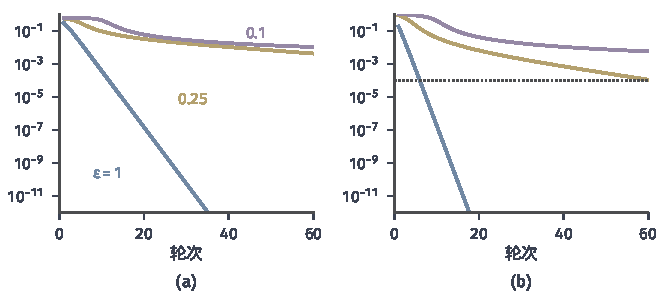
\includegraphics[width=112mm]{figures/07-probability/07-distribution-optimization/matplotlib/ot-sinkhorn-convergence/figure.pdf}
 \caption{全章例子上对数域Sinkhorn迭代的收敛，纵轴为对数刻度：$\varepsilon=1$（蓝）、$0.25$（黄）、$0.1$（紫）。(a)行残差$\rho^{(t)}$。(b)修正后可行方案的原对偶差$\Delta^{(t)}$，深灰点线为容差$10^{-4}$。}
 \label{fig:ot-sinkhorn-convergence}
\end{BookInlineFigure}

\paragraph{三种误差}
用熵正则化近似一个分布之间的运输问题时，最终结果与真正的$\operatorname{OT}_c(\mu,\nu)$之间有三种误差，应分别记录。离散化误差来自把$\mu,\nu$换成有限网格或有限样本上的分布，它取决于网格尺度或样本数。正则化偏差由式~\eqref{eq:ot-entropic-bias}控制，随$\varepsilon$线性减小。迭代误差由停止判据式~\eqref{eq:ot-sinkhorn-stop}控制。减小$\varepsilon$能降低偏差，却使迭代变慢、对数域计算变得必要；三者要在同一预算下权衡，不能只报告其中一项。若最终需要的是原问题的运输成本，还要报告$\langle\bm{C},\tilde{\bm{\pi}}\rangle$而不是正则化目标值。

\section{分布插值}
\label{sec:ot-interpolation}

给定两个分布$\mu_0,\mu_1$，怎样在它们之间连一条路径$\mu_t$，$0\leq t\leq1$？最直接的是混合$(1-t)\mu_0+t\mu_1$：质量不动，只是把权重从一个分布渐渐挪到另一个。取$\mu_0=\delta_0$，$\mu_1=\delta_1$，混合路径在中途是$\tfrac12\delta_0+\tfrac12\delta_1$，一半质量在$0$、一半在$1$，中间位置$\tfrac12$上什么也没有。若把分布想成一堆土，更自然的中途状态是“土堆搬到了一半的路上”，即$\delta_{1/2}$。最优运输给出这种路径：沿最优耦合把每份质量匀速推向它的目的地。

\begin{definition}[位移插值]
\label{def:ot-displacement}
设$\mu_0,\mu_1$是$\mathbb{R}^{d}$上具有有限二阶矩的分布，$\pi$是它们在平方欧氏成本下的一个最优耦合。对$0\leq t\leq1$，令$e_t(x,y)=(1-t)x+ty$，称
\begin{equation}
 \mu_t=(e_t)_\#\pi
 \label{eq:ot-displacement}
\end{equation}
为沿$\pi$的\term{位移插值}（displacement interpolation）。
\end{definition}

用随机向量说，取$(X,Y)\sim\pi$，$\mu_t$就是$(1-t)X+tY$的分布：每份质量从$X$出发，沿直线匀速走到$Y$，$t$时刻走完全程的$t$。$e_0,e_1$是两个坐标投影，所以端点正是$\mu_0,\mu_1$。$(1-t)x+ty$的平方范数不超过$2\lVert x\rVert_2^{2}+2\lVert y\rVert_2^{2}$，所以$\mu_t$也有有限二阶矩。

\begin{theorem}[位移插值是常速测地线]
\label{thm:ot-geodesic}
在定义~\ref{def:ot-displacement}的条件下，对一切$0\leq s\leq t\leq1$，
\begin{equation}
 W_2(\mu_s,\mu_t)=(t-s)\,W_2(\mu_0,\mu_1).
 \label{eq:ot-geodesic}
\end{equation}
\end{theorem}

\begin{proof}
记$W=W_2(\mu_0,\mu_1)$，$(X,Y)\sim\pi$。$\bigl((1-s)X+sY,\ (1-t)X+tY\bigr)$是$\mu_s$与$\mu_t$的一个耦合，两分量之差为$(t-s)(Y-X)$，所以
\[
 W_2^{2}(\mu_s,\mu_t)\leq(t-s)^{2}\,\mathbb{E}\lVert X-Y\rVert_2^{2}=(t-s)^{2}W^{2} .
\]
同样得到$W_2(\mu_0,\mu_s)\leq sW$，$W_2(\mu_t,\mu_1)\leq(1-t)W$。由$W_2$的三角不等式（第~\ref{chap:distribution-comparison}章），
\[
 \begin{aligned}
 W&\leq W_2(\mu_0,\mu_s)+W_2(\mu_s,\mu_t)+W_2(\mu_t,\mu_1)\\
 &\leq sW+(t-s)W+(1-t)W=W .
 \end{aligned}
\]
两端相等，中间每个不等号都必须取等，于是式~\eqref{eq:ot-geodesic}成立。
\end{proof}

式~\eqref{eq:ot-geodesic}说的是：$t\mapsto\mu_t$在度量$W_2$下走的是一条最短路，并且匀速，称为常速\term{测地线}（geodesic）。沿路径任意两点之间的距离恰好等于参数之差乘以全长，路径上不存在任何绕路。

\paragraph{两个点质量}
$\delta_0$与$\delta_1$之间只有一个耦合，位移插值是$\mu_t=\delta_t$，$W_2(\mu_s,\mu_t)=t-s$。混合路径$\nu_t=(1-t)\delta_0+t\delta_1$完全不同。$\nu_s$与$\nu_t$都在$\{0,1\}$上，它们在点$1$处的质量相差$t-s$，任何耦合至少要让这么多质量在$0$与$1$之间移动距离$1$；把恰好$t-s$的质量从$0$搬到$1$就做到了，所以
\[
 W_2(\nu_s,\nu_t)=\sqrt{t-s} .
\]
它不与$t-s$成正比。把$[0,1]$等分成$n$段，混合路径各段的$W_2$长度之和是$n\cdot\sqrt{1/n}=\sqrt{n}\to\infty$：按位置度量，混合路径根本不是一条有限长的路。图~\ref{fig:ot-point-interp}(a)对比了两种中途状态。

\begin{BookInlineFigure}
 \centering
 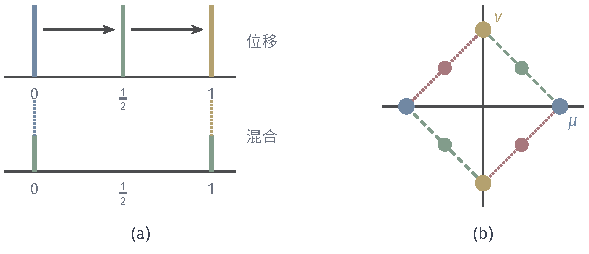
\includegraphics[width=108mm]{figures/07-probability/07-distribution-optimization/tikz/ot-point-interp/figure.pdf}
 \caption{位移插值与混合。(a)$\delta_0$（蓝）与$\delta_1$（黄）在$t=\tfrac12$的中途状态：上行是位移插值$\delta_{1/2}$，下行是混合$\tfrac12\delta_0+\tfrac12\delta_1$，竖线高度表示质量。(b)$\mu=\tfrac12(\delta_{(1,0)}+\delta_{(-1,0)})$（蓝）与$\nu=\tfrac12(\delta_{(0,1)}+\delta_{(0,-1)})$（黄），任何耦合都最优；绿色与红色分别是两个不同最优耦合的中点。}
 \label{fig:ot-point-interp}
\end{BookInlineFigure}

\paragraph{全章例子}
逐格搬运是平方成本下唯一的最优方案。$t=\tfrac12$时，留在$0$与$2$的质量不动，从$0$搬往$1$的$0.3$走到$0.5$，从$1$搬往$2$的$0.3$走到$1.5$：
\[
 \mu_{1/2}=0.2\,\delta_0+0.3\,\delta_{0.5}+0.3\,\delta_{1.5}+0.2\,\delta_2 .
\]
它与两端的距离都是$\tfrac12W_2=\tfrac12\sqrt{0.6}\approx0.387$。同一时刻的混合是$0.35\,\delta_0+0.3\,\delta_1+0.35\,\delta_2$，仍只放在原来的三个位置上。

\paragraph{一维高斯分布}
$\mu_0=\mathcal{N}(m_0,\sigma_0^{2})$与$\mu_1=\mathcal{N}(m_1,\sigma_1^{2})$之间的最优映射是$T(x)=m_1+(\sigma_1/\sigma_0)(x-m_0)$。取$X\sim\mu_0$，
\[
 (1-t)X+tT(X)=(1-t)m_0+tm_1+\Bigl((1-t)+t\frac{\sigma_1}{\sigma_0}\Bigr)(X-m_0),
\]
所以
\begin{equation}
 \mu_t=\mathcal{N}\Bigl((1-t)m_0+tm_1,\ \bigl((1-t)\sigma_0+t\sigma_1\bigr)^{2}\Bigr).
 \label{eq:ot-gaussian-geodesic}
\end{equation}
均值与标准差都线性变化，路径上始终是单峰的高斯分布。混合路径在中途是双峰的。图~\ref{fig:ot-displacement}取$m_0=-2$，$\sigma_0=0.5$，$m_1=2$，$\sigma_1=1$，画出两条路径。

\begin{BookInlineFigure}
 \centering
 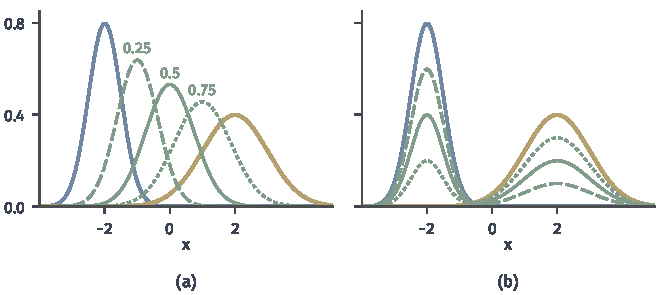
\includegraphics[width=112mm]{figures/07-probability/07-distribution-optimization/matplotlib/ot-displacement/figure.pdf}
 \caption{$\mathcal{N}(-2,0.5^{2})$（蓝）与$\mathcal{N}(2,1)$（黄）之间的两条路径，绿线是$t=0.25$（虚线）、$0.5$（实线）、$0.75$（点线）时的密度。(a)位移插值，密度整体平移并逐渐变宽。(b)混合，两个峰原地不动，只是高度此消彼长。}
 \label{fig:ot-displacement}
\end{BookInlineFigure}

\paragraph{插值不唯一}
定义~\ref{def:ot-displacement}依赖所选的最优耦合。最优耦合不唯一时，插值也不唯一。在$\mathbb{R}^{2}$中取
\[
 \mu=\tfrac12\bigl(\delta_{(1,0)}+\delta_{(-1,0)}\bigr),\qquad \nu=\tfrac12\bigl(\delta_{(0,1)}+\delta_{(0,-1)}\bigr).
\]
四个源—目标点对的平方距离都是$2$，所以每个耦合的成本都是$2$，全部最优。把$(1,0)$送到$(0,1)$、$(-1,0)$送到$(0,-1)$，中点落在$(\tfrac12,\tfrac12)$与$(-\tfrac12,-\tfrac12)$；交换目的地，中点落在另一条对角线上；独立耦合则在四个中点上各放$\tfrac14$。三者都是$\mu$与$\nu$之间的常速测地线在$t=\tfrac12$处的状态，见图~\ref{fig:ot-point-interp}(b)。

若$\mu_0$关于Lebesgue测度绝对连续，平方成本下的最优耦合唯一，并且由某个凸函数$\phi$的梯度给出：$\pi=(\mathrm{id},\nabla\phi)_\#\mu_0$。这时插值也唯一：
\[
 \mu_t=\bigl((1-t)\mathrm{id}+t\nabla\phi\bigr)_\#\mu_0 .
\]第~\ref{sec:ot-gaussian}节的对称正定线性映射就是$\phi$为二次函数的情形。一般情形的证明要用凸函数的几乎处处可微性，可查阅~\scite{math-villani2009transport}。

\section{Wasserstein重心}
\label{sec:ot-barycenter}

上一节在两个分布之间取中途状态。有多个分布时，能否找一个分布共同代表它们？对点$x_1,\dots,x_K\in\mathbb{R}^{d}$与权重$\lambda_k$，加权平均$\bar{x}=\sum_k\lambda_kx_k$是使$\sum_k\lambda_k\lVert y-x_k\rVert_2^{2}$最小的点。把点换成分布、把平方距离换成$W_2^{2}$，就得到分布的“平均”。

\begin{definition}[Wasserstein重心]
\label{def:ot-barycenter}
设$\mu_1,\dots,\mu_K$是$\mathbb{R}^{d}$上具有有限二阶矩的分布，权重$\lambda_k\geq0$，$\sum_k\lambda_k=1$。在有限二阶矩的分布$\nu$中最小化
\begin{equation}
 \Psi(\nu)=\sum_{k=1}^{K}\lambda_kW_2^{2}(\nu,\mu_k),
 \label{eq:ot-barycenter}
\end{equation}
最小点称为$\mu_1,\dots,\mu_K$关于这组权重的\term{Wasserstein重心}（Wasserstein barycenter）。
\end{definition}

它与混合分布$\sum_k\lambda_k\mu_k$是两回事。混合把各分布的质量按权重叠在一起，质量都留在原处；重心则把质量搬到“平均位置”上。

\paragraph{点质量的重心}
取$\mu_k=\delta_{x_k}$。任何$\nu$与点质量只有一个耦合，即$\nu\otimes\delta_{x_k}$，所以
\[
 W_2^{2}(\nu,\delta_{x_k})=\int\lVert y-x_k\rVert_2^{2}\,\nu(\mathrm{d}y).
\]对每个$y$有恒等式
\[
 \sum_k\lambda_k\lVert y-x_k\rVert_2^{2}=\lVert y-\bar{x}\rVert_2^{2}+\sum_k\lambda_k\lVert x_k-\bar{x}\rVert_2^{2},
\]
因为交叉项$2\sum_k\lambda_k\langle y-\bar{x},\bar{x}-x_k\rangle$中$\sum_k\lambda_k(\bar{x}-x_k)=0$。对$\nu$积分，
\[
 \Psi(\nu)=\int\lVert y-\bar{x}\rVert_2^{2}\,\nu(\mathrm{d}y)+\sum_k\lambda_k\lVert x_k-\bar{x}\rVert_2^{2},
\]
第一项在且仅在$\nu=\delta_{\bar{x}}$时为零。所以点质量的重心唯一，是$\delta_{\bar{x}}$，正是点的加权平均；混合分布$\sum_k\lambda_k\delta_{x_k}$则在每个$x_k$上各放一份质量。

\paragraph{两个分布的重心}
$K=2$、权重$(1-t,t)$时，位移插值$\mu_t$是重心。记$W=W_2(\mu_0,\mu_1)$，任取$\nu$，令$\alpha=W_2(\nu,\mu_0)$，$\beta=W_2(\nu,\mu_1)$，由三角不等式$\alpha+\beta\geq W$。直接展开可以验证
\[
 (1-t)\alpha^{2}+t\beta^{2}-t(1-t)(\alpha+\beta)^{2}=\bigl((1-t)\alpha-t\beta\bigr)^{2}\geq0 ,
\]
所以$\Psi(\nu)\geq t(1-t)W^{2}$。由定理~\ref{thm:ot-geodesic}，$\mu_t$满足$\alpha=tW$，$\beta=(1-t)W$，代入得
\[
 \Psi(\mu_t)=(1-t)t^{2}W^{2}+t(1-t)^{2}W^{2}=t(1-t)W^{2},
\]
达到下界。

\paragraph{实数轴上的重心}
一维时，由定理~\ref{thm:ot-one-dimensional}，$W_2^{2}$是分位数函数之差的平方积分，重心问题化为分位数函数的最小二乘。

\begin{theorem}[一维重心]
\label{thm:ot-barycenter-1d}
设$\mu_1,\dots,\mu_K$是实数轴上具有有限二阶矩的分布，分位数函数为$F_k^{-1}$。则重心唯一，它的分位数函数是
\begin{equation}
 \bar{q}(u)=\sum_{k=1}^{K}\lambda_kF_k^{-1}(u),\qquad0<u<1 .
 \label{eq:ot-barycenter-1d}
\end{equation}
\end{theorem}

\begin{proof}
任取有限二阶矩的分布$\nu$，分位数函数为$G^{-1}$。由式~\eqref{eq:ot-quantile-formula}与点质量情形中的同一恒等式（逐个$u$使用），
\[
 \Psi(\nu)=\int_0^{1}\bigl(G^{-1}(u)-\bar{q}(u)\bigr)^{2}\,\mathrm{d}u+\sum_k\lambda_k\int_0^{1}\bigl(F_k^{-1}(u)-\bar{q}(u)\bigr)^{2}\,\mathrm{d}u .
\]
第二项与$\nu$无关。$\bar{q}$是单调不减、左连续函数的非负组合，仍单调不减且左连续；由各$F_k^{-1}$平方可积，它也平方可积。令$\bar{\nu}$为$\bar{q}(U)$的分布，$U\sim\operatorname{Unif}(0,1)$，由单调性与左连续性可以验证$\bar{\nu}$的分位数函数就是$\bar{q}$，并且$\bar{\nu}$有有限二阶矩。于是$\bar{\nu}$使第一项为零，是重心。反过来，任何重心都使第一项为零，$G^{-1}=\bar{q}$几乎处处成立；两个左连续单调函数几乎处处相等就处处相等，所以重心就是$\bar{\nu}$。
\end{proof}

对一维高斯分布$\mu_k=\mathcal{N}(m_k,\sigma_k^{2})$，$F_k^{-1}(u)=m_k+\sigma_k\Phi^{-1}(u)$，其中$\Phi$是标准高斯分布函数，于是重心是
\[
 \mathcal{N}\Bigl(\sum_k\lambda_km_k,\ \bigl(\textstyle\sum_k\lambda_k\sigma_k\bigr)^{2}\Bigr):
\]
均值平均，标准差也平均。图~\ref{fig:ot-barycenter}取三个形状不同的分布，$\mathcal{N}(-3,0.5^{2})$、$\operatorname{Unif}(-1,1)$与$\mathcal{N}(3.5,0.8^{2})$，权重各$\tfrac13$。重心的分位数函数是
\[
 \bar{q}(u)=\tfrac13\bigl(-0.5+1.3\,\Phi^{-1}(u)+2u\bigr),
\]
均值为$\tfrac16$，形状介于高斯与均匀之间，是一个单峰分布；混合分布则保留三个分开的峰。

\begin{BookInlineFigure}
 \centering
 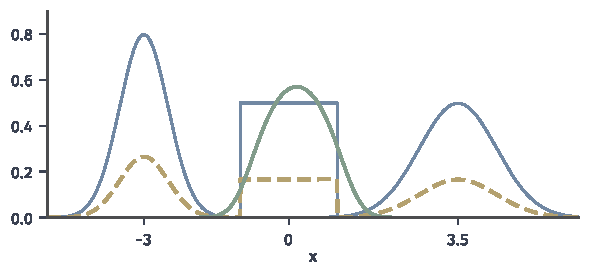
\includegraphics[width=100mm]{figures/07-probability/07-distribution-optimization/matplotlib/ot-barycenter/figure.pdf}
 \caption{三个分布（蓝）：$\mathcal{N}(-3,0.5^{2})$、$\operatorname{Unif}(-1,1)$、$\mathcal{N}(3.5,0.8^{2})$，权重各$\tfrac13$。绿线是Wasserstein重心的密度，由平均分位数函数式~\eqref{eq:ot-barycenter-1d}数值求得；黄色虚线是混合分布的密度。}
 \label{fig:ot-barycenter}
\end{BookInlineFigure}

\paragraph{存在与唯一}
一般维数中没有分位数可用，但存在性可以沿用第~\ref{sec:ot-existence}节的紧性论证。

\begin{theorem}[重心的存在]
\label{thm:ot-barycenter-existence}
在定义~\ref{def:ot-barycenter}的条件下，重心存在。
\end{theorem}

\begin{proof}
记$V=\inf_\nu\Psi(\nu)$，取$\nu=\mu_1$知$V<\infty$。取有限二阶矩的分布列$\nu_l$，使$\Psi(\nu_l)\to V$。

\emph{二阶矩一致有界。}取$\lambda_{k_0}>0$。$\lVert y\rVert_2^{2}$不超过$2\lVert y-x\rVert_2^{2}+2\lVert x\rVert_2^{2}$，在$\nu_l$与$\mu_{k_0}$的最优耦合下取期望，
\[
 \int\lVert y\rVert_2^{2}\,\nu_l(\mathrm{d}y)\leq\frac{2\Psi(\nu_l)}{\lambda_{k_0}}+2\int\lVert x\rVert_2^{2}\,\mu_{k_0}(\mathrm{d}x),
\]
右边对$l$有界，记为$M$。由第~\ref{chap:weak-convergence-of-distributions}章的矩条件，$\{\nu_l\}$胎紧，有子列（仍记为$\nu_l$）弱收敛到某个$\nu$。对每个$R>0$，$\min(\lVert y\rVert_2^{2},R)$有界连续，其积分在极限中不超过$M$；令$R\to\infty$，$\nu$的二阶矩不超过$M$。

\emph{距离下半连续。}固定$k$，取子列使$W_2^{2}(\nu_l,\mu_k)$趋于它的下极限，取最优耦合$\pi_l\in\Pi(\nu_l,\mu_k)$。$\{\nu_l\}$与$\mu_k$都胎紧，按引理~\ref{lem:ot-coupling-compact}的证明，$\{\pi_l\}$胎紧，再取子列使$\pi_l\xrightarrow{\mathrm{w}}\pi$。对有界连续的$h$，
\[
 \int h(x)\,\pi(\mathrm{d}x,\mathrm{d}y)=\lim_{l\to\infty}\int h\,\mathrm{d}\nu_l=\int h\,\mathrm{d}\nu ,
\]
所以$\pi$的第一边缘是$\nu$；每个$\pi_l$的第二边缘都是$\mu_k$，同样的论证说明$\pi$的第二边缘也是$\mu_k$。由引理~\ref{lem:ot-cost-lsc}，
\[
 W_2^{2}(\nu,\mu_k)\leq\int\lVert x-y\rVert_2^{2}\,\mathrm{d}\pi\leq\liminf_{l\to\infty}W_2^{2}(\nu_l,\mu_k).
\]
对$k$加权求和，下极限之和不超过和的下极限，于是$\Psi(\nu)\leq\liminf_l\Psi(\nu_l)=V$。
\end{proof}

唯一性需要额外条件。若某个权重为正的$\mu_k$关于Lebesgue测度绝对连续，重心唯一。机制是：这时$\nu\mapsto W_2^{2}(\nu,\mu_k)$在分布的混合下严格凸，而$\Psi$的其余各项是凸的；严格凸性来自第~\ref{sec:ot-interpolation}节提到的最优耦合由凸函数梯度唯一给出，证明可查阅前面提到的Villani的专著。条件不能随意去掉。在第~\ref{sec:ot-interpolation}节的正方形例子中取权重$(\tfrac12,\tfrac12)$，两个分布都是点质量组成的，不绝对连续；三种不同的中途状态都满足$\alpha=\beta=\tfrac12W$，都使$\Psi$达到下界$\tfrac14W^{2}$，所以重心不唯一。一维情形是例外，定理~\ref{thm:ot-barycenter-1d}对任何有限二阶矩的分布都给出唯一性。

\section{本章小结}
\label{sec:ot-summary}

本章从一个问题出发：两个边缘分布固定，怎样把一个搬成另一个最省。可行方案是全部耦合，它们构成一个凸集；在有限情形是运输多面体，在一般情形靠固定边缘带来的胎紧性获得紧性。成本非负下半连续时最优耦合存在；去掉下半连续，极小化序列可能在极限处跳高。存在的是最优耦合，不是最优映射：映射要求质量不可拆分，可能连可行解都没有，或者下确界取不到。

最优性的证据来自对偶。满足$\varphi(x)+\psi(y)\leq c(x,y)$的一对势给出一切耦合成本的公共下界，原对偶差等于耦合下松弛量的积分，所以质量只落在零松弛处的耦合就是最优的。有限情形的强对偶由线性规划得到，紧致空间上的连续成本可以由有限问题逼近得到；原问题达到、无对偶间隙与最优势存在是三个不同的结论，需要分别核对条件。

具体结构决定怎样求解。表~\ref{tab:ot-summary}汇总本章求解的几类问题。

\begin{table}[htbp]
 \centering
 \caption{本章求解的运输问题。高斯两行为平方成本，实数轴一行要求$p\geq1$与有限$p$阶矩；“映射”一列指最优方案是否由运输映射实现。}
 \label{tab:ot-summary}
 \begin{tabular}{lll}
  \toprule
  问题 & 最优方案 & 映射\\
  \midrule
  实数轴，$\lvert x-y\rvert^{p}$ & 分位数耦合 & 源无原子时是\\
  有限支持 & 线性规划的顶点 & 一般不是\\
  高斯，$\bm{\Sigma}_1$正定 & 对称正定仿射映射 & 是\\
  高斯，$\bm{\Sigma}_1$奇异 & 按支撑子空间分析 & 可能不是\\
  熵正则化 & 行列缩放式~\eqref{eq:ot-scaling-form} & 不是\\
  \bottomrule
 \end{tabular}
\end{table}

一维问题证明了第~\ref{chap:distribution-comparison}章提到的关系：$W_1$等于两条分布函数之间的面积，$W_p^{p}$等于分位数函数之差的$p$次方积分。全章例子中，逐格搬运同时被对偶势、分位数耦合证实为平方成本下唯一的最优方案，成本$0.6$。熵正则化把运输问题变成严格凸的光滑问题，解具有行列缩放形式，Sinkhorn迭代交替满足行和与列和；正则化偏差不超过$\varepsilon$乘以最优方案与独立方案之间的KL散度，迭代误差由修正可行方案后的原对偶差控制，两者与离散化误差要分别报告。

最后两节用最优耦合构造新的分布。位移插值把每份质量沿直线匀速推向目的地，是$W_2$下的常速测地线；混合路径则只调整权重，在$W_2$下甚至不是有限长的路径。Wasserstein重心推广了点的加权平均，在有限二阶矩下存在；一维时就是分位数函数的加权平均，高维时唯一性需要某个正权重分布绝对连续。最优耦合不唯一时，插值与重心都不唯一。

本章始终在成本、矩条件、映射可行性与数值误差的范围内下结论：有限$p$阶矩保证成本有限，下半连续保证最优耦合存在，严格凸成本与绝对连续的源分布才带来唯一性与映射，正则化与迭代给出的是带有可计算误差界的近似。$W_p$作为距离的性质及其与弱收敛的关系，分别见第~\ref{chap:distribution-comparison}章与第~\ref{chap:weak-convergence-of-distributions}章。


